\chapter{Results and Analysis}

We executed our library functions on the onion data. This data consists of 
Wholesale Price, Retail Price and Arrival since 1st January 2006 to 6th July 
2015. In this chapter, we will show results produced by our system and will 
analyse these results along with each method.

\section{Results}

We have performed 4 types of analysis and result for each of this method is as 
follows. Note that these are primary results. Data for 2 centres are considered 
- Mumbai and Delhi.\\
\\
Here are some results related with Mumbai Center. Table \ref{AnomaliesReported} shows the result of anomalies reported by our system, with details about anomalies reported by each method. So here First 5 columns corresponds to each method. Column 6 is union of results of first 3 methods and column 7 is union of results of method 4 and 5, as described in table. Column 8 is intersection of results of column 6 and column 7, which is final result of our system.\\
\\
Table \ref{ArticlesMatched} shows the result of number of articles matched with the dates reported by our system as anomaly for each method. So here First 5 columns corresponds to each method. Column 6 is union of results of first 3 methods and column 7 is union of result of method 4 and 5, as described in table. Column 8 is intersection of results of column 6 and column 7, which is final result of our system.\\
\\
Note that total number of articles present for center Mumbai is \textbf{99} and all these articles are present after 2010. Apart from Graph Based Anomaly and Multivariate- vector autoregressive method, all methods are producing results from 2006 onwards as input data is from that time. The following pie chart(see figure \ref{fig:pieReasons}) shows the analysis of article showing what news articles states as the reason for the price hikes of onion.\\
\\
\begin{figure}[H]
\centering
\begin{tikzpicture}
   \pie[ text = legend ]{32/Traders Nexus, 18/Not Stated, 10/Unseasonal Rainfall, 12/Low Production, 18/Low Supply, 10/Other  }
\end{tikzpicture}
\caption{Reasons stated by news articles for onion price hike}
\label{fig:pieReasons}
\end{figure}

% First here about +5, -5

While finding the news article match for every anomaly, we check for all the news articles 5 days before and 5 days after the reported date. In case we find any news article in this tenure, we consider it as a match for that date. For one date of anomaly, multiple articles may be present but for this analysis we have considered only the nearest article for that anomaly date. Following bar charts represents distribution of how far is the news article from the date of anomaly.

\begin{figure}[H]
\centering
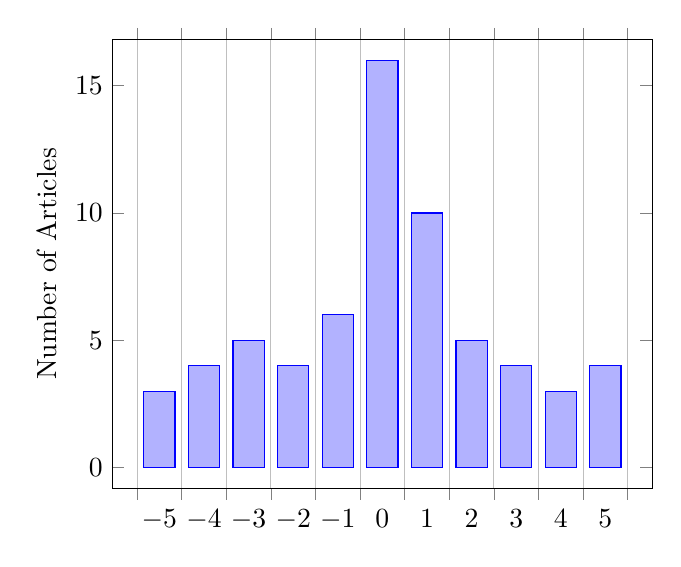
\begin{tikzpicture}
\begin{axis}[
	x tick label style={
		/pgf/number format/1000 sep=},
	ylabel=Number of Articles,
	enlargelimits=0.05,
	legend style={at={(0.5,-0.1)},
	anchor=north,legend columns=-1},
	ybar interval=0.7,
]
\addplot 
	coordinates {(-5,3)(-4,4)(-3,5)(-2,4)(-1,6)(0,16)(1,10)(2,5)(3,4)(4,3)(5,4)(6,0)};

\end{axis}
\end{tikzpicture}
\caption{Article Distribution for Retail Price VS Average Retail Price}
\label{fig:articleDistRvsR}
\end{figure}

\begin{figure}[H]
\centering
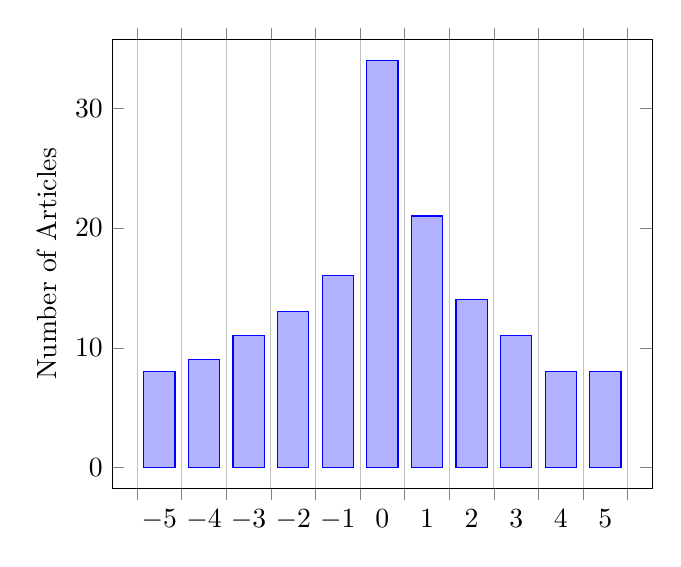
\begin{tikzpicture}
\begin{axis}[
	x tick label style={
		/pgf/number format/1000 sep=},
	ylabel=Number of Articles,
	enlargelimits=0.05,
	legend style={at={(0.5,-0.1)},
	anchor=north,legend columns=-1},
	ybar interval=0.7,
]
\addplot 
	coordinates {(-5,8)(-4,9)(-3,11)(-2,13)(-1,16)(0,34)(1,21)(2,14)(3,11)(4,8)(5,8)(6,0)};

% \legend{Men,Women}
\end{axis}
\end{tikzpicture}
\caption{Article Distribution for Retail Price VS Arrival Of Onion}
\label{fig:articleDistRvsA}
\end{figure}


\begin{figure}[H]
\centering
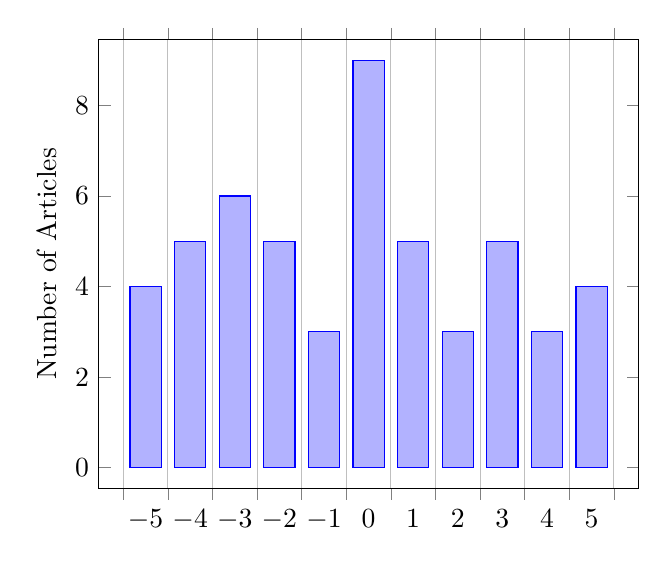
\begin{tikzpicture}
\begin{axis}[
	x tick label style={
		/pgf/number format/1000 sep=},
	ylabel=Number of Articles,
	enlargelimits=0.05,
	legend style={at={(0.5,-0.1)},
	anchor=north,legend columns=-1},
	ybar interval=0.7,
]
\addplot 
	coordinates {(-5,4)(-4,5)(-3,6)(-2,5)(-1,3)(0,9)(1,5)(2,3)(3,5)(4,3)(5,4)(6,0)};

% \legend{Men,Women}
\end{axis}
\end{tikzpicture}
\caption{Article Distribution for Wholesale Price VS Retail Price}
\label{fig:articleDistRvsW}
\end{figure}


\begin{figure}[H]
\centering
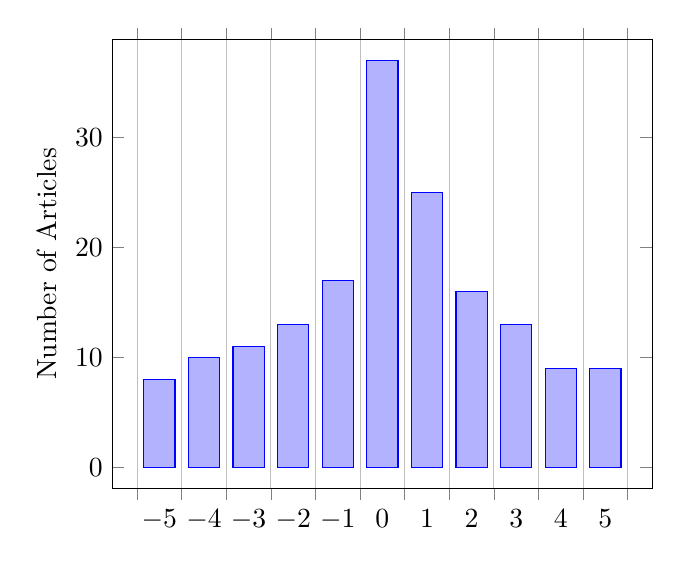
\begin{tikzpicture}
\begin{axis}[
	x tick label style={
		/pgf/number format/1000 sep=},
	ylabel=Number of Articles,
	enlargelimits=0.05,
	legend style={at={(0.5,-0.1)},
	anchor=north,legend columns=-1},
	ybar interval=0.7,
]
\addplot 
	coordinates {(-5,8)(-4,10)(-3,11)(-2,13)(-1,17)(0,37)(1,25)(2,16)(3,13)(4,9)(5,9)(6,0)};

% \legend{Men,Women}
\end{axis}
\end{tikzpicture}
\caption{Article Distribution for Wholesale Price VS Arrival Of Onion}
\label{fig:articleDistWvsA}
\end{figure}


Now, we present detailed analysis for each of the different type of time-series. First type of such analysis is in table \ref{RetailVsAverage}. This table shows distribution of news articles present (that matched with system results) year-wise for each method when retail price time series is compared with average retail price time series. Second type of such analysis is in table \ref{RetailVsArrival}. This table shows distribution of news articles present year-wise for each method when retail price time series is compared with arrival data of onion time series. Third type of such analysis is in table \ref{RetailVsWholesale}. This table shows distribution of news articles present year-wise for each method when retail price time series is compared with wholesale price time series. Fourth type of such analysis is in table \ref{WholesaleVsArrival}. This table shows distribution of news articles present year-wise for each method when wholesale price time series is compared with arrival data of onion time series.\\
\\
Distribution of anomalies present year-wise, for each method is also shown in table. Result for various analysis is described in tables  \ref{RetailVsAverageDist}, \ref{RetailVsArrivalDist}, \ref{RetailVsWholesaleDist} and \ref{WholesaleVsArrivalDist}.\\
\\
Such results for different cities can also be calculated.

  
	\begin{table}[]
	\centering
	
	\resizebox{\textwidth}{!}
	{\begin{tabular}{|l|l|l|l|l|l|l|l|l|}
	\hline
	Methods              & Slope Based (1) & Correlation (2) & Linear Regression (3) & Graph Based (4) & Multivariate (5) & 1 U 2 U 3 (6) & 4 U 5 (7) & 6 $\cap$ 7  \\
	\hline
	Retail Vs Average    & 742 & 255 & 353 & 300 & 177 & 1206 & 362 & 125 \\
	\hline
	Retail Vs Arrival    & 420 & 795 & 353 & 500 & 167 & 1381 & 573 & 323 \\
	\hline
	Retail Vs Wholesale  & 658 & 420 & 310 & 300 & 167 & 1243 & 367 & 160 \\
	\hline
	Wholesale Vs Arrival & 448 & 705 & 282 & 500 & 186 & 1315 & 586 & 332 \\
	\hline
	\end{tabular}}
	\caption{Anomalies Reported}
	\label{AnomaliesReported}
	\end{table}
      
	\begin{table}[]
	\centering
	
	\resizebox{\textwidth}{!}
	{\begin{tabular}{|l|l|l|l|l|l|l|l|l|}
	\hline
	Methods              & Slope Based (1) & Correlation (2) & Linear Regression (3) & Graph Based (4) & Multivariate (5) & 1 U 2 U 3 (6) & 4 U 5 (7) & 6 $\cap$ 7   \\
	\hline
	Retail Vs Average    & 67 & 47 & 50  & 122 & 122 & 142 & 162 & 64  \\
	\hline
	Retail Vs Arrival    & 42 & 74 & 167 & 121 & 119 & 220 & 159 & 153 \\
	\hline
	Retail Vs Wholesale  & 30 & 55 & 40  & 117 & 119 & 107 & 150 & 52  \\
	\hline
	Wholesale Vs Arrival & 64 & 64 & 174 & 122 & 139 & 219 & 174 & 168 \\
	\hline
	\end{tabular}}
	\caption{Number of news articles matched with system}
	\label{ArticlesMatched}
	\end{table}
	
      

	\begin{table}[]
	\centering
	\resizebox{\textwidth}{!}
	{\begin{tabular}{|l|l|l|l|l|l|l|l|l|l|}
	\hline
	Distribution of All Articles & Articles Present & Slope Based (1) & Correlation (2) & Linear Regression (3) & Graph Based (4) & Multivariate (5) & 1 U 2 U 3 (6) & 4 U 5 (7) & 6 $\cap$ 7 \\
	\hline
	2010 & 6  & 0  & 0  & 8  & 10 & 0   & 8  & 10  & 3  \\
	\hline
	2011 & 3  & 0  & 0  & 0  & 12 & 0   & 0  & 12  & 0  \\
	\hline
	2012 & 2  & 1  & 0  & 0  & 0  & 0   & 1  & 0   & 0  \\
	\hline
	2013 & 54 & 42 & 14 & 18 & 86 & 119 & 61 & 125 & 61 \\
	\hline
	2014 & 23 & 24 & 0  & 24 & 14 & 3   & 39 & 15  & 0  \\
	\hline
	2015 & 11 & 0  & 33 & 0  & 0  & 0   & 33 & 0   & 0  \\
	\hline
	\end{tabular}}	
	\caption{Retail Price VS Average Retail Price}
	\label{RetailVsAverage}
	\end{table}
	
	
	
	\begin{table}[]
	\centering
	\resizebox{\textwidth}{!}
	{\begin{tabular}{|l|l|l|l|l|l|l|l|l|l|}
	\hline
	Distribution of All Articles & Articles Present & Slope Based (1) & Correlation (2) & Linear Regression (3) & Graph Based (4) & Multivariate (5) & 1 U 2 U 3 (6) & 4 U 5 (7) & 6 $\cap$ 7  \\
	\hline
	2010 & 6  & 17 & 0  & 17  & 17 & 0   & 17  & 17  & 17  \\
	\hline
	2011 & 3  & 1  & 0  & 12  & 12 & 0   & 12  & 12  & 12  \\
	\hline
	2012 & 2  & 0  & 0  & 0   & 0  & 0   & 0   & 0   & 0   \\
	\hline
	2013 & 54 & 10 & 39 & 126 & 92 & 119 & 137 & 130 & 124 \\
	\hline
	2014 & 23 & 14 & 35 & 12  & 0  & 0   & 54  & 0   & 0   \\
	\hline
	2015 & 11 & 0  & 0  & 0   & 0  & 0   & 0   & 0   & 0  \\
	\hline
	\end{tabular}}	
	\caption{Retail Price VS Arrival data of onion}
	\label{RetailVsArrival}
	\end{table}

	
	
	
	\begin{table}[]
	\centering
	\resizebox{\textwidth}{!}
	{\begin{tabular}{|l|l|l|l|l|l|l|l|l|l|}
	\hline
	Distribution of All Articles & Articles Present & Slope Based (1) & Correlation (2) & Linear Regression (3) & Graph Based (4) & Multivariate (5) & 1 U 2 U 3 (6) & 4 U 5 (7) & 6 $\cap$ 7 \\
	\hline
	2010 & 6  & 6  & 0  & 2  & 11 & 0   & 6  & 11  & 6  \\
	\hline
	2011 & 3  & 1  & 0  & 0  & 4  & 0   & 1  & 4   & 1  \\
	\hline
	2012 & 2  & 2  & 7  & 0  & 0  & 0   & 7  & 0   & 0  \\
	\hline
	2013 & 54 & 7  & 21 & 18 & 91 & 119 & 45 & 124 & 44 \\
	\hline
	2014 & 23 & 14 & 27 & 20 & 11 & 0   & 48 & 11  & 1  \\
	\hline
	2015 & 11 & 0  & 0  & 0  & 0  & 0   & 0  & 0   & 0 \\
	\hline
	\end{tabular}}	
	\caption{Retail Price VS Wholesale Price}
	\label{RetailVsWholesale}
	\end{table}

	
	
	\begin{table}[]
	\centering
	\resizebox{\textwidth}{!}
	{\begin{tabular}{|l|l|l|l|l|l|l|l|l|l|}
	\hline
	Distribution of All Articles & Articles Present & Slope Based (1) & Correlation (2) & Linear Regression (3) & Graph Based (4) & Multivariate (5) & 1 U 2 U 3 (6) & 4 U 5 (7) & 6 $\cap$ 7  \\
	\hline
	2010 & 6  & 17 & 0  & 17  & 17 & 0   & 17  & 17  & 17  \\
	\hline
	2011 & 3  & 1  & 0  & 12  & 12 & 0   & 12  & 12  & 12  \\
	\hline
	2012 & 2  & 0  & 0  & 0   & 0  & 0   & 0   & 0   & 0   \\
	\hline
	2013 & 54 & 25 & 15 & 125 & 93 & 123 & 129 & 129 & 123 \\
	\hline
	2014 & 23 & 21 & 49 & 20  & 0  & 16  & 61  & 16  & 16  \\
	\hline
	2015 & 11 & 0  & 0  & 0   & 0  & 0   & 0   & 0   & 0   \\
	\hline
	\end{tabular}}	
	\caption{ Wholesale Price VS Arrival data of onion}
	\label{WholesaleVsArrival}
	\end{table}
	
	
	
	
	\begin{table}[]
	\centering
	\resizebox{\textwidth}{!}
	{\begin{tabular}{|l|l|l|l|l|l|l|l|l|}
	\hline
	Distribution of All Articles & Slope Based (1) & Correlation (2) & Linear Regression (3) & Graph Based (4) & Multivariate (5) & 1 U 2 U 3 (6) & 4 U 5 (7) & 6 $\cap$ 7 \\
	\hline
	2006 & 133 & 30 & 65  & 0   & 0   & 204 & 0   & 0  \\
	\hline
	2007 & 14  & 15 & 30  & 0   & 0   & 53  & 0   & 0  \\
	\hline
	2008 & 42  & 15 & 0   & 0   & 0   & 47  & 0   & 0  \\
	\hline
	2009 & 82  & 15 & 0   & 0   & 0   & 96  & 0   & 0  \\
	\hline
	2010 & 72  & 45 & 28  & 37  & 0   & 142 & 37  & 13 \\
	\hline
	2011 & 56  & 60 & 115 & 57  & 0   & 182 & 57  & 9  \\
	\hline
	2012 & 84  & 0  & 33  & 13  & 0   & 100 & 13  & 5  \\
	\hline
	2013 & 77  & 15 & 56  & 134 & 161 & 125 & 189 & 90 \\
	\hline
	2014 & 140 & 0  & 26  & 40  & 16  & 155 & 47  & 8  \\
	\hline
	2015 & 42  & 60 & 0   & 19  & 0   & 102 & 19  & 0  \\
	\hline
	\end{tabular}}
	\caption{Distribution of Anomalies reported by system for Retail Price VS Average Retail Price}
	\label{RetailVsAverageDist}
	\end{table}
	  
	  
	  
	
	\begin{table}[]
	\centering
	\resizebox{\textwidth}{!}
	{\begin{tabular}{|l|l|l|l|l|l|l|l|l|}
	\hline
	Distribution of All Articles & Slope Based (1) & Correlation (2) & Linear Regression (3) & Graph Based (4) & Multivariate (5) & 1 U 2 U 3 (6) & 4 U 5 (7) & 6 $\cap$ 7  \\
	\hline
	2006 & 35 & 185 & 0   & 0   & 0   & 199 & 0   & 0   \\
	\hline
	2007 & 63 & 85  & 0   & 0   & 0   & 148 & 0   & 0   \\
	\hline
	2008 & 28 & 105 & 0   & 0   & 0   & 126 & 0   & 0   \\
	\hline
	2009 & 28 & 45  & 0   & 0   & 0   & 73  & 0   & 0   \\
	\hline
	2010 & 48 & 60  & 46  & 143 & 0   & 107 & 143 & 56  \\
	\hline
	2011 & 36 & 60  & 40  & 165 & 0   & 128 & 165 & 65  \\
	\hline
	2012 & 77 & 45  & 0   & 81  & 0   & 118 & 81  & 25  \\
	\hline
	2013 & 59 & 90  & 168 & 111 & 161 & 263 & 178 & 172 \\
	\hline
	2014 & 46 & 105 & 99  & 0   & 6   & 204 & 6   & 5   \\
	\hline
	2015 & 0  & 15  & 0   & 0   & 0   & 15  & 0   & 0   \\
	\hline
	\end{tabular}}
	\caption{Distribution of Anomalies reported by system for Retail Price VS Arrival data of onion }
	\label{RetailVsArrivalDist}
	\end{table}
	
	
	\begin{table}[]
	\centering
	\resizebox{\textwidth}{!}
	{\begin{tabular}{|l|l|l|l|l|l|l|l|l|}
	\hline
	Distribution of All Articles & Slope Based (1) & Correlation (2) & Linear Regression (3) & Graph Based (4) & Multivariate (5) & 1 U 2 U 3 (6) & 4 U 5 (7) & 6 $\cap$ 7  \\
	\hline
	2006 & 126 & 0  & 0  & 0   & 0   & 126 & 0   & 0  \\
	\hline
	2007 & 77  & 30 & 0  & 0   & 0   & 107 & 0   & 0  \\
	\hline
	2008 & 70  & 15 & 0  & 0   & 0   & 85  & 0   & 0  \\
	\hline
	2009 & 63  & 75 & 0  & 0   & 0   & 126 & 0   & 0  \\
	\hline
	2010 & 62  & 30 & 2  & 53  & 0   & 92  & 53  & 8  \\
	\hline
	2011 & 50  & 45 & 67 & 75  & 0   & 155 & 75  & 34 \\
	\hline
	2012 & 72  & 82 & 64 & 7   & 0   & 160 & 7   & 0  \\
	\hline
	2013 & 50  & 38 & 44 & 105 & 161 & 124 & 166 & 81 \\
	\hline
	2014 & 60  & 75 & 99 & 60  & 6   & 182 & 66  & 37 \\
	\hline
	2015 & 28  & 30 & 34 & 0   & 0   & 86  & 0   & 0  \\
	\hline
	\end{tabular}}
	\caption{Distribution of Anomalies reported by system for Retail Price VS Wholesale Price }
	\label{RetailVsWholesaleDist}
	\end{table}
	
	
	\begin{table}[]
	\centering
	\resizebox{\textwidth}{!}
	{\begin{tabular}{|l|l|l|l|l|l|l|l|l|}
	\hline
	Distribution of All Articles & Slope Based (1) & Correlation (2) & Linear Regression (3) & Graph Based (4) & Multivariate (5) & 1 U 2 U 3 (6) & 4 U 5 (7) & 6 $\cap$ 7  \\
	\hline
	2006 & 0  & 65  & 0   & 0   & 0   & 65  & 0   & 0   \\
	\hline
	2007 & 42 & 100 & 0   & 0   & 0   & 142 & 0   & 0   \\
	\hline
	2008 & 21 & 120 & 0   & 0   & 0   & 141 & 0   & 0   \\
	\hline
	2009 & 56 & 60  & 0   & 0   & 0   & 109 & 0   & 0   \\
	\hline
	2010 & 83 & 75  & 51  & 142 & 0   & 162 & 142 & 62  \\
	\hline
	2011 & 64 & 60  & 34  & 165 & 0   & 157 & 165 & 67  \\
	\hline
	2012 & 42 & 45  & 0   & 81  & 0   & 87  & 81  & 12  \\
	\hline
	2013 & 80 & 45  & 157 & 112 & 152 & 246 & 164 & 157 \\
	\hline
	2014 & 46 & 105 & 40  & 0   & 34  & 162 & 34  & 34  \\
	\hline
	2015 & 14 & 30  & 0   & 0   & 0   & 44  & 0   & 0   \\
	\hline
	\end{tabular}}
	\caption{Distribution of Anomalies reported by system for Wholesale Price VS Arrival data of onion }
	\label{WholesaleVsArrivalDist}
	\end{table}
	

\section{Analysis of Each Method}

In this section, we try to analyse strengths, weaknesses and limitations of every method. So, we will describe each method one by one. Note that we have articles from 2010 onwards, so we will be focussing on anomalies reported after 2010 and compare them with the news articles we have. \\
\\
\textbf{Note that all the graphs and results described in following sections are for centre Mumbai. Mumbai is in Maharashtra state, which is the largest producer of onion in India. Also in graphs, Yellow highlighted region corresponds to anomalies reported by system, red region corresponds to dates for which our system reported anomaly and news article was present for that and blue region corresponds to date for which news article was present but that date was not reported as anomaly by our system.}

\subsection{Slope Based Anomaly Detection}
	
		The main functionality of this method is to find change in one variable with respect to other. Given two time-series, here we try to find, between two points in time series, how much dependent variable changed corresponding to independent variable. If this change is huge, then it is reported as anomaly.\\
		\\
		We have four types of analysis which are as following:
		\begin{enumerate}
			\item \textbf{Retail Price vs Average of Retail Price}: Here, we first take average of retail price at all centres and than compare change in retail price with respect to change in average of retail price for different time window.			
			\item \textbf{Retail Price vs Arrival of Onion}: Here, we try to find change in retail price with respect to change in arrival of onion for different windows. 
			\item \textbf{Retail Price vs Wholesale Price}: Here, retail price is dependent on wholesale price and we try to find change in retail price with respect to change wholesale price for different windows.
			\item \textbf{Wholesale Price vs Arrival of Onion}: Here, we try to find change in wholesale price with respect to change in arrival of onion for different window size.
		\end{enumerate}
		
		So, in each of the case, we try to find change with respect to another, and if this change is huge, crossing threshold than it is reported as anomaly. Note that in analysis 1 and 3 stated above, both the time series are directly proportional to each other and in the analysis 2 and 4 both the time series are inversely proportional to each other. So, limitations faced by this method for analysis 1 and 3 will be similar and for analysis 2 and 4 will be similar. While describing this method, each analysis will be referenced by its corresponding number.\\
		\\
		First we will start with analysis 1 and 3. Following are the few observations:
		
			
		\begin{itemize}
		
			\item In case of analysis 1, dates are reported as anomalies if retail price at centre is increasing more as compared to average retail price and in case of analysis 3, it is reported if retail price at centre is increasing more as compared to wholesale price. \\
			Following tenures are some cases reported by this method:
			\begin{itemize}
				\item \textit{Analysis 1}: June 2010, August 2010, May 2011, June 2011, May Jun Nov 2012, Apr May 2013 (Prices went too high as compared to average) (See Figure \ref{fig:12111})
				\item \textit{Analysis 3}: Apr July Oct Dec 2010, Jan 2011, May June 2014 (See Figure \ref{fig:12131})
			\end{itemize}
			\begin{figure}[H]
		    	\centering
  		    	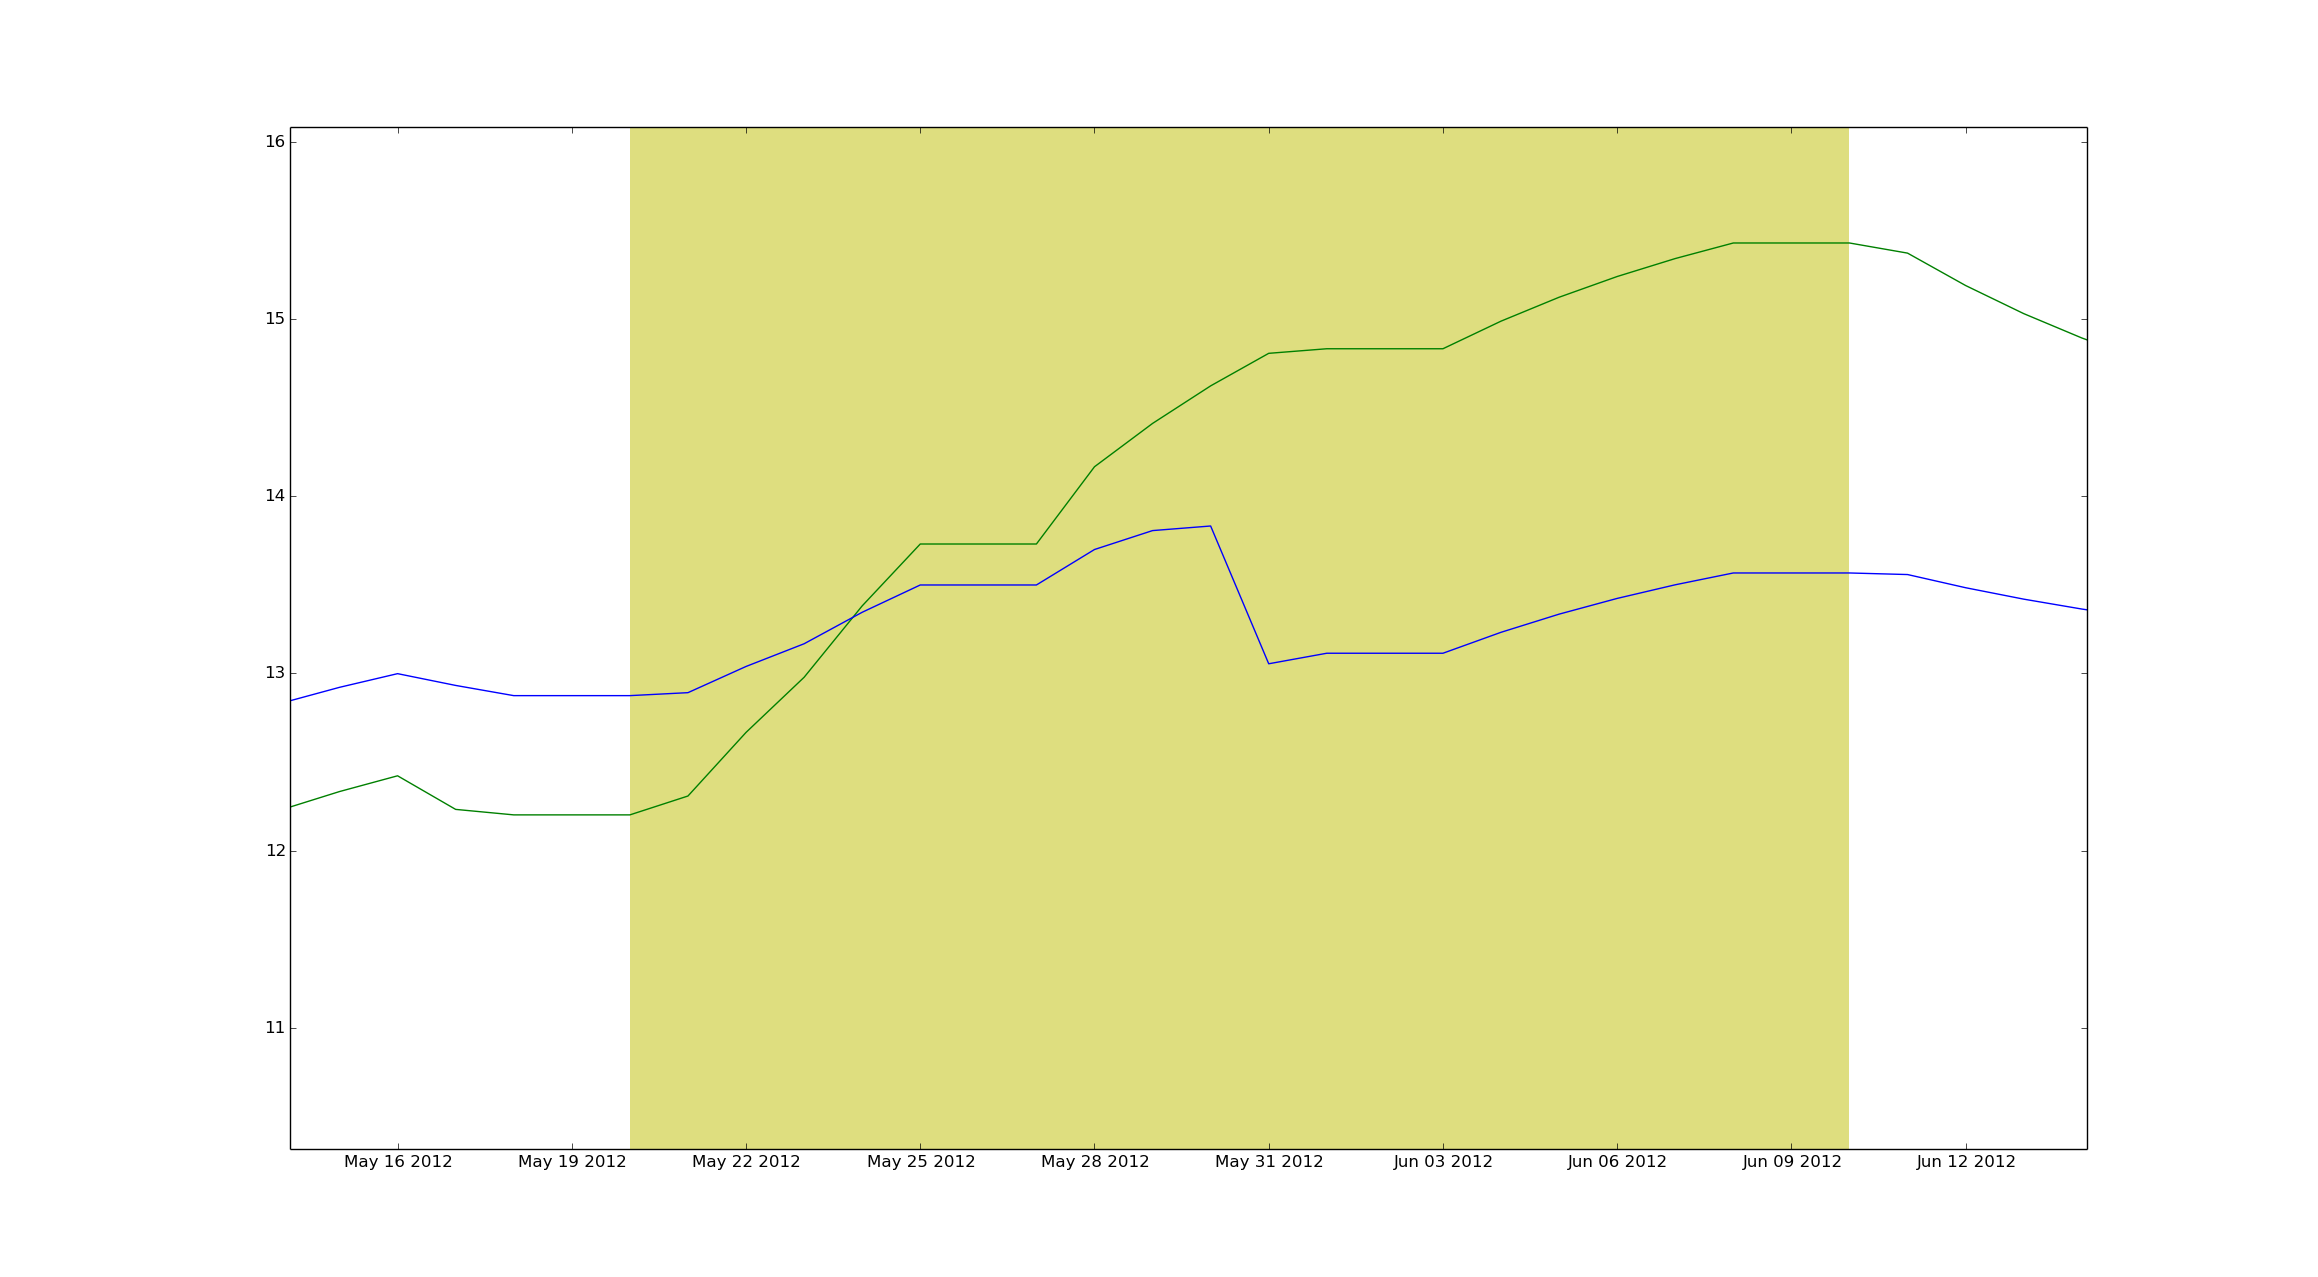
\includegraphics[width=0.8\textwidth]{graphs/12111.png}
		    	\caption{Slope Based Anomaly Detection (Green line - Centre Retail Price, Blue Line - Average Retail Price)}
		    	\label{fig:12111}
			\end{figure}
			
			\begin{figure}[H]
		    	\centering
  		    	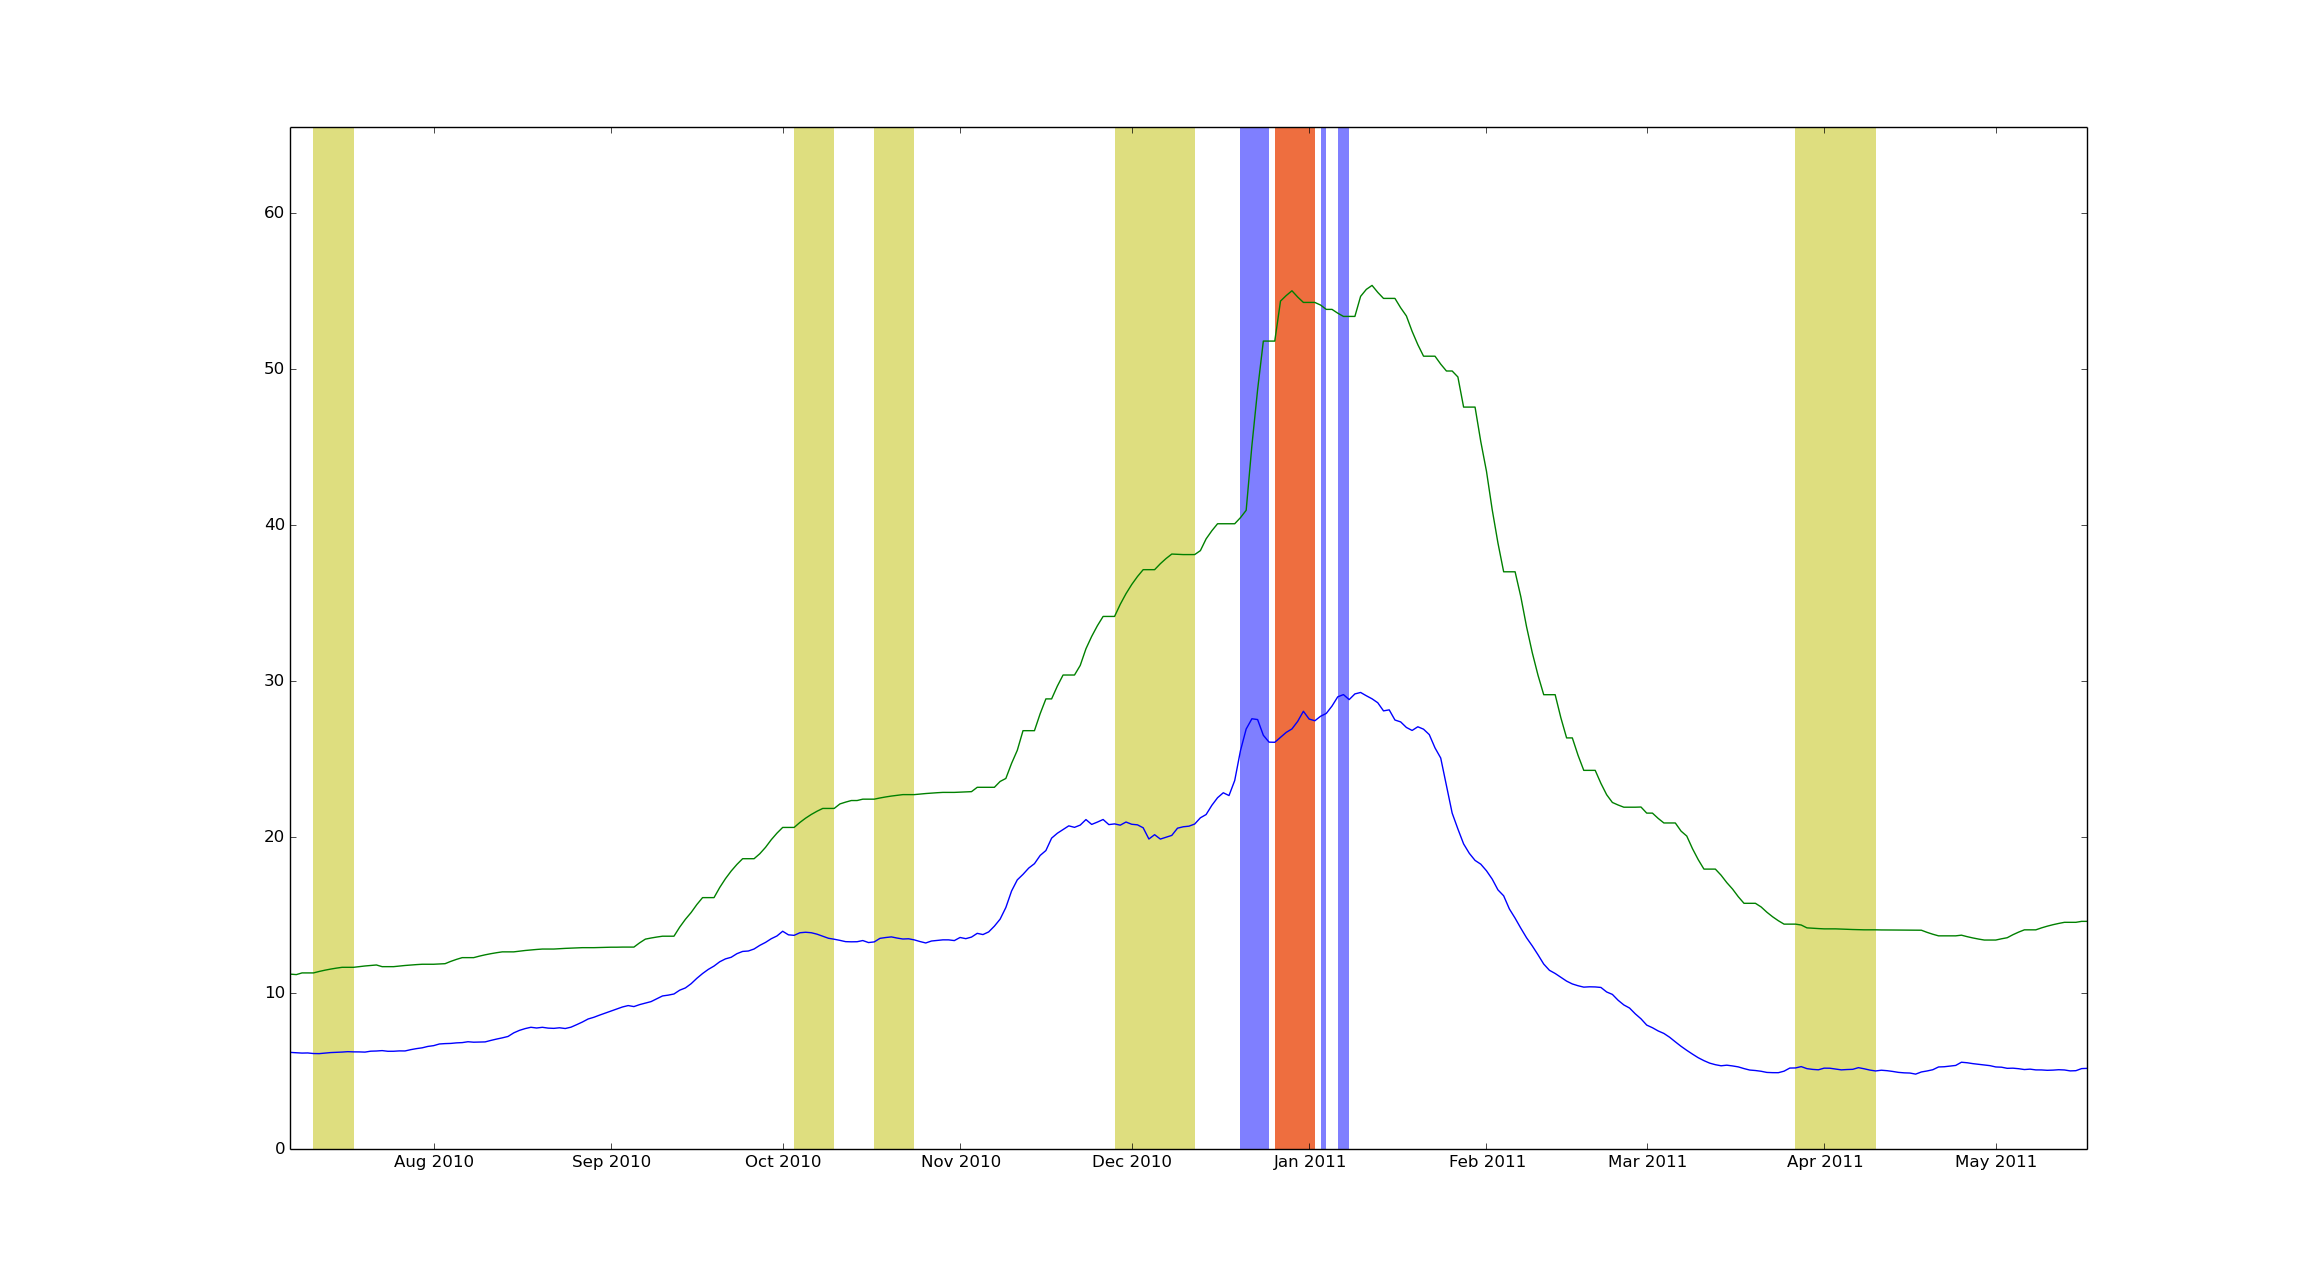
\includegraphics[width=0.8\textwidth]{graphs/12131.png}
		    	\caption{Slope Based Anomaly Detection (Green line - Retail Price, Blue Line - Wholesale Price)}
		    	\label{fig:12131}
			\end{figure}
			
			
			
			So, even though we do not have articles for these anomalies, but method is behaving as it should be. 			
			
			\item One of the limitation for this method is that there are some cases where drop in retail price for one center is quite huge as compared to drop in average retail price (in case of \textit{analysis 1}) or wholesale price (in case of \textit{analysis 3}). This is good thing for customers at that centre and should not be treated as anomaly. But in this case, slope value goes high and that's why our method reports that tenure as anomaly.\\
			Following tenures are some cases reported by this method:
			\begin{itemize}
				\item \textit{Analysis 1}: January 2010, June Aug 2012, Jan 2013, Feb Oct 2014, Feb 2015  (See Figure \ref{fig:12112})
				\item \textit{Analysis 3}: Feb May 2010  (See Figure \ref{fig:12132})
			\end{itemize}
			
			\begin{figure}[H]
		    	\centering
  		    	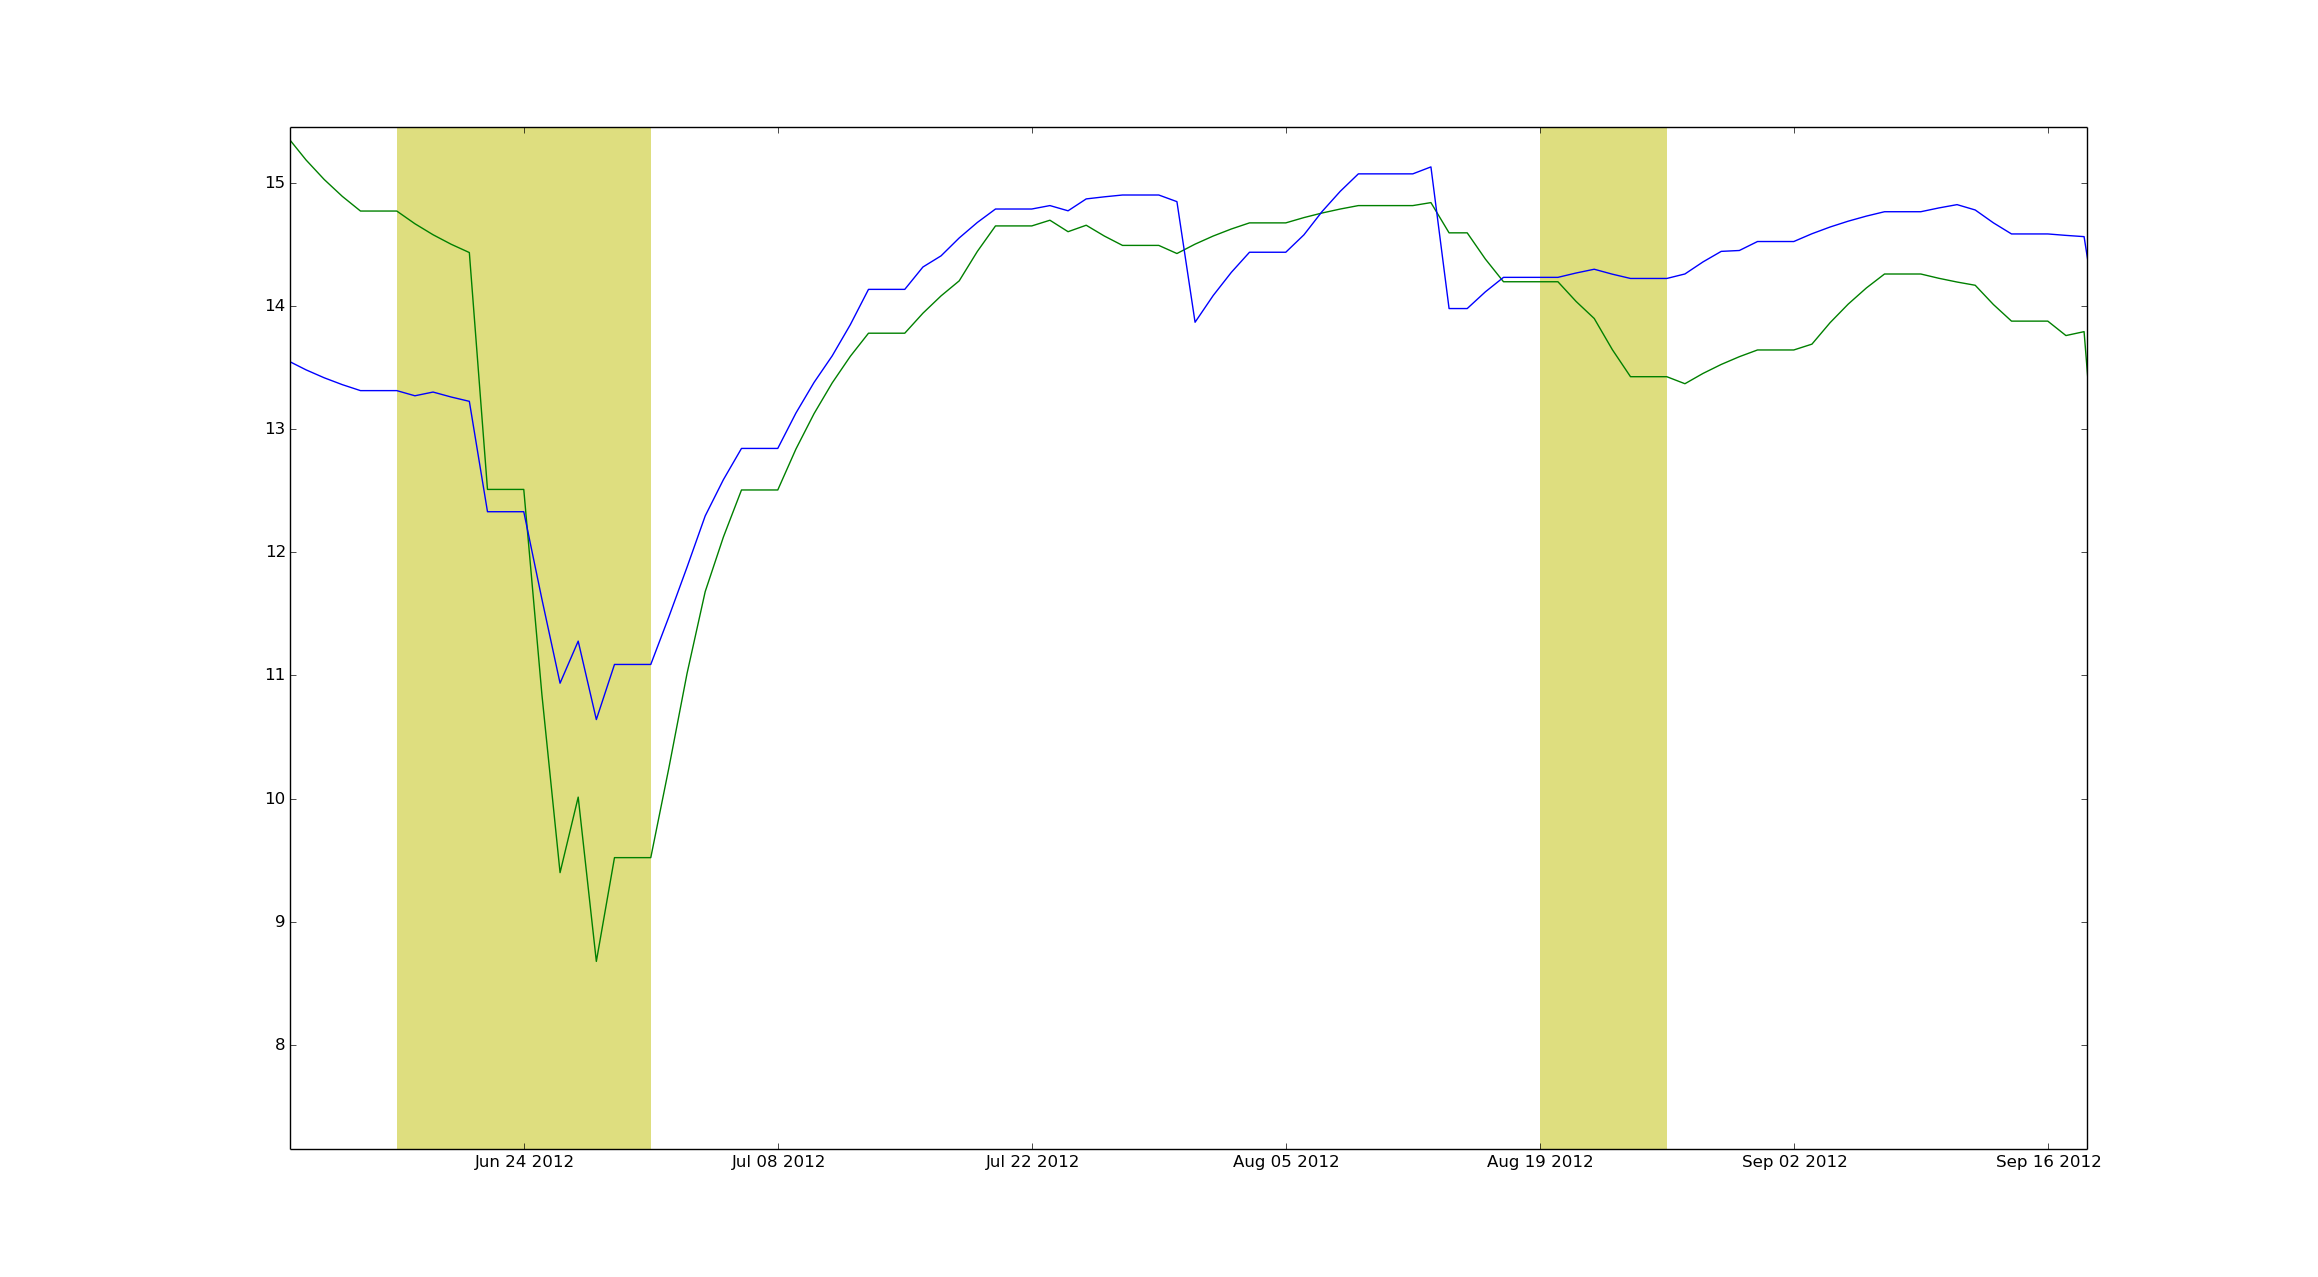
\includegraphics[width=0.8\textwidth]{graphs/12112.png}
		    	\caption{Slope Based Anomaly Detection (Green line - Centre Retail Price, Blue Line - Average Retail Price)}
		    	\label{fig:12112}
			\end{figure}
			
			\begin{figure}[H]
		    	\centering
  		    	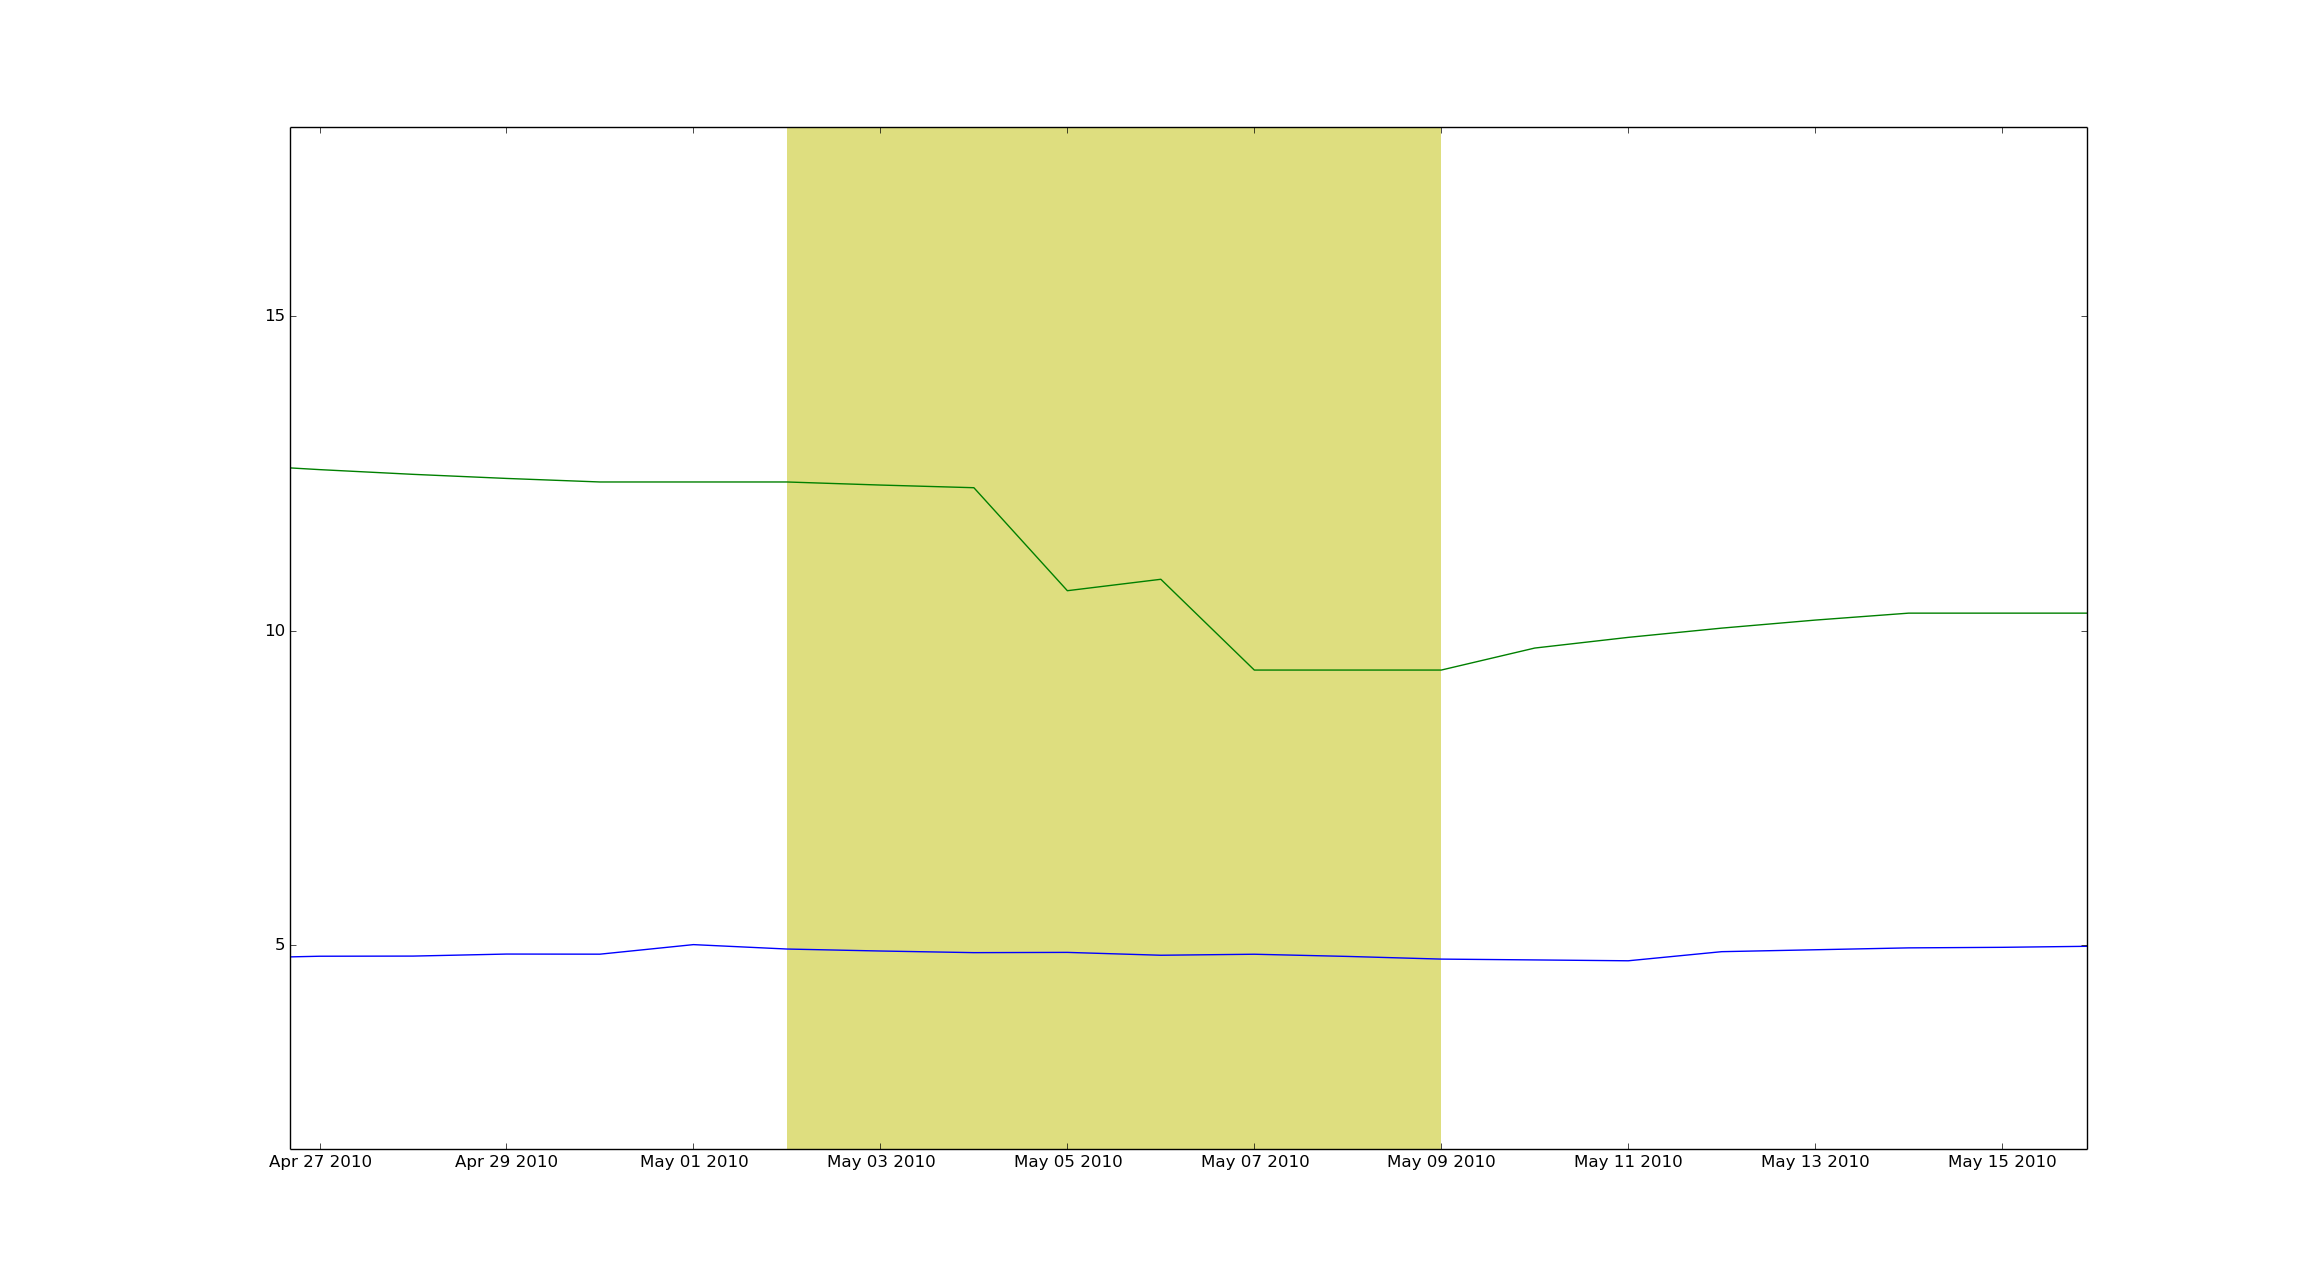
\includegraphics[width=0.8\textwidth]{graphs/12132.png}
		    	\caption{Slope Based Anomaly Detection (Green line - Retail Price, Blue Line - Wholesale Price)}
		    	\label{fig:12132}
			\end{figure}
						
			
			
			
			
			\item Other observation is related to why few anomalies were reported in news but not by our system. Reason for that is we are comparing relative change in two time series. Now for some dates, where news article is present but our system did not report, value of both time series increased together. Although, prices went too high, but still relative change, i.e. slope value remained relatively low as compared to others. So that was not reported by our system.
				
			Following tenures are some cases reported by this method:
			\begin{itemize}
				\item \textit{Analysis 1}: Dec 2010, Jan Feb 2012, June 2013, May June 2015   (See Figure \ref{fig:12113})
				\item \textit{Analysis 3}: Feb 2013, July 2014   (See Figure \ref{fig:12133})
			\end{itemize}
			
			\begin{figure}[H]
		    	\centering
  		    	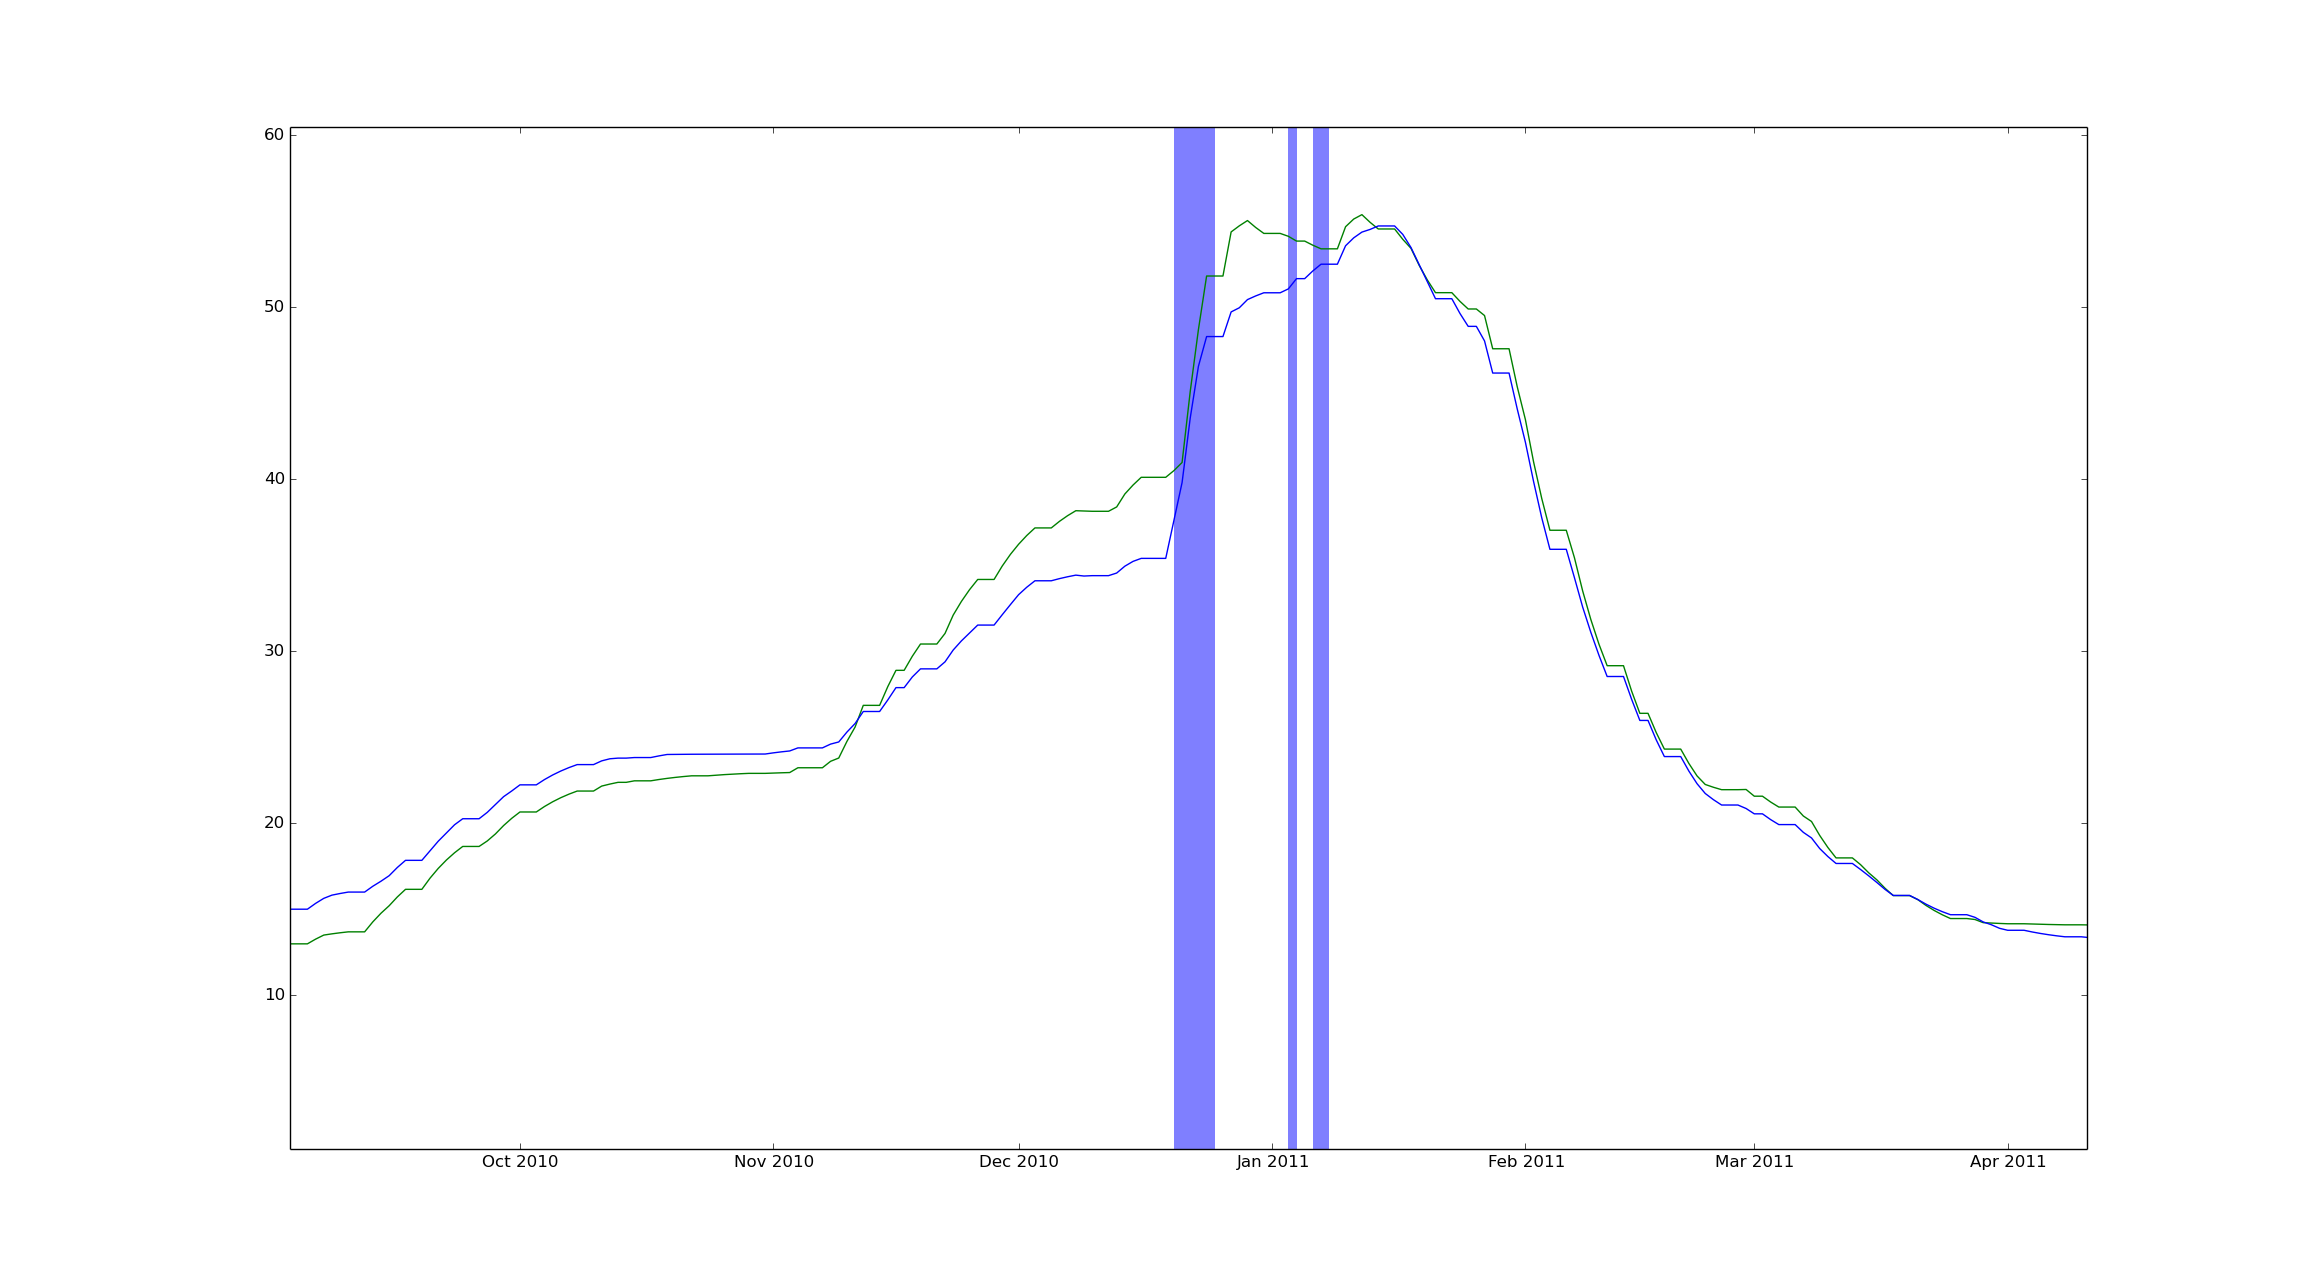
\includegraphics[width=0.8\textwidth]{graphs/12113.png}
		    	\caption{Slope Based Anomaly Detection (Green line - Centre Retail Price, Blue Line - Average Retail Price)}
		    	\label{fig:12113}
			\end{figure}
			
			\begin{figure}[H]
		    	\centering
  		    	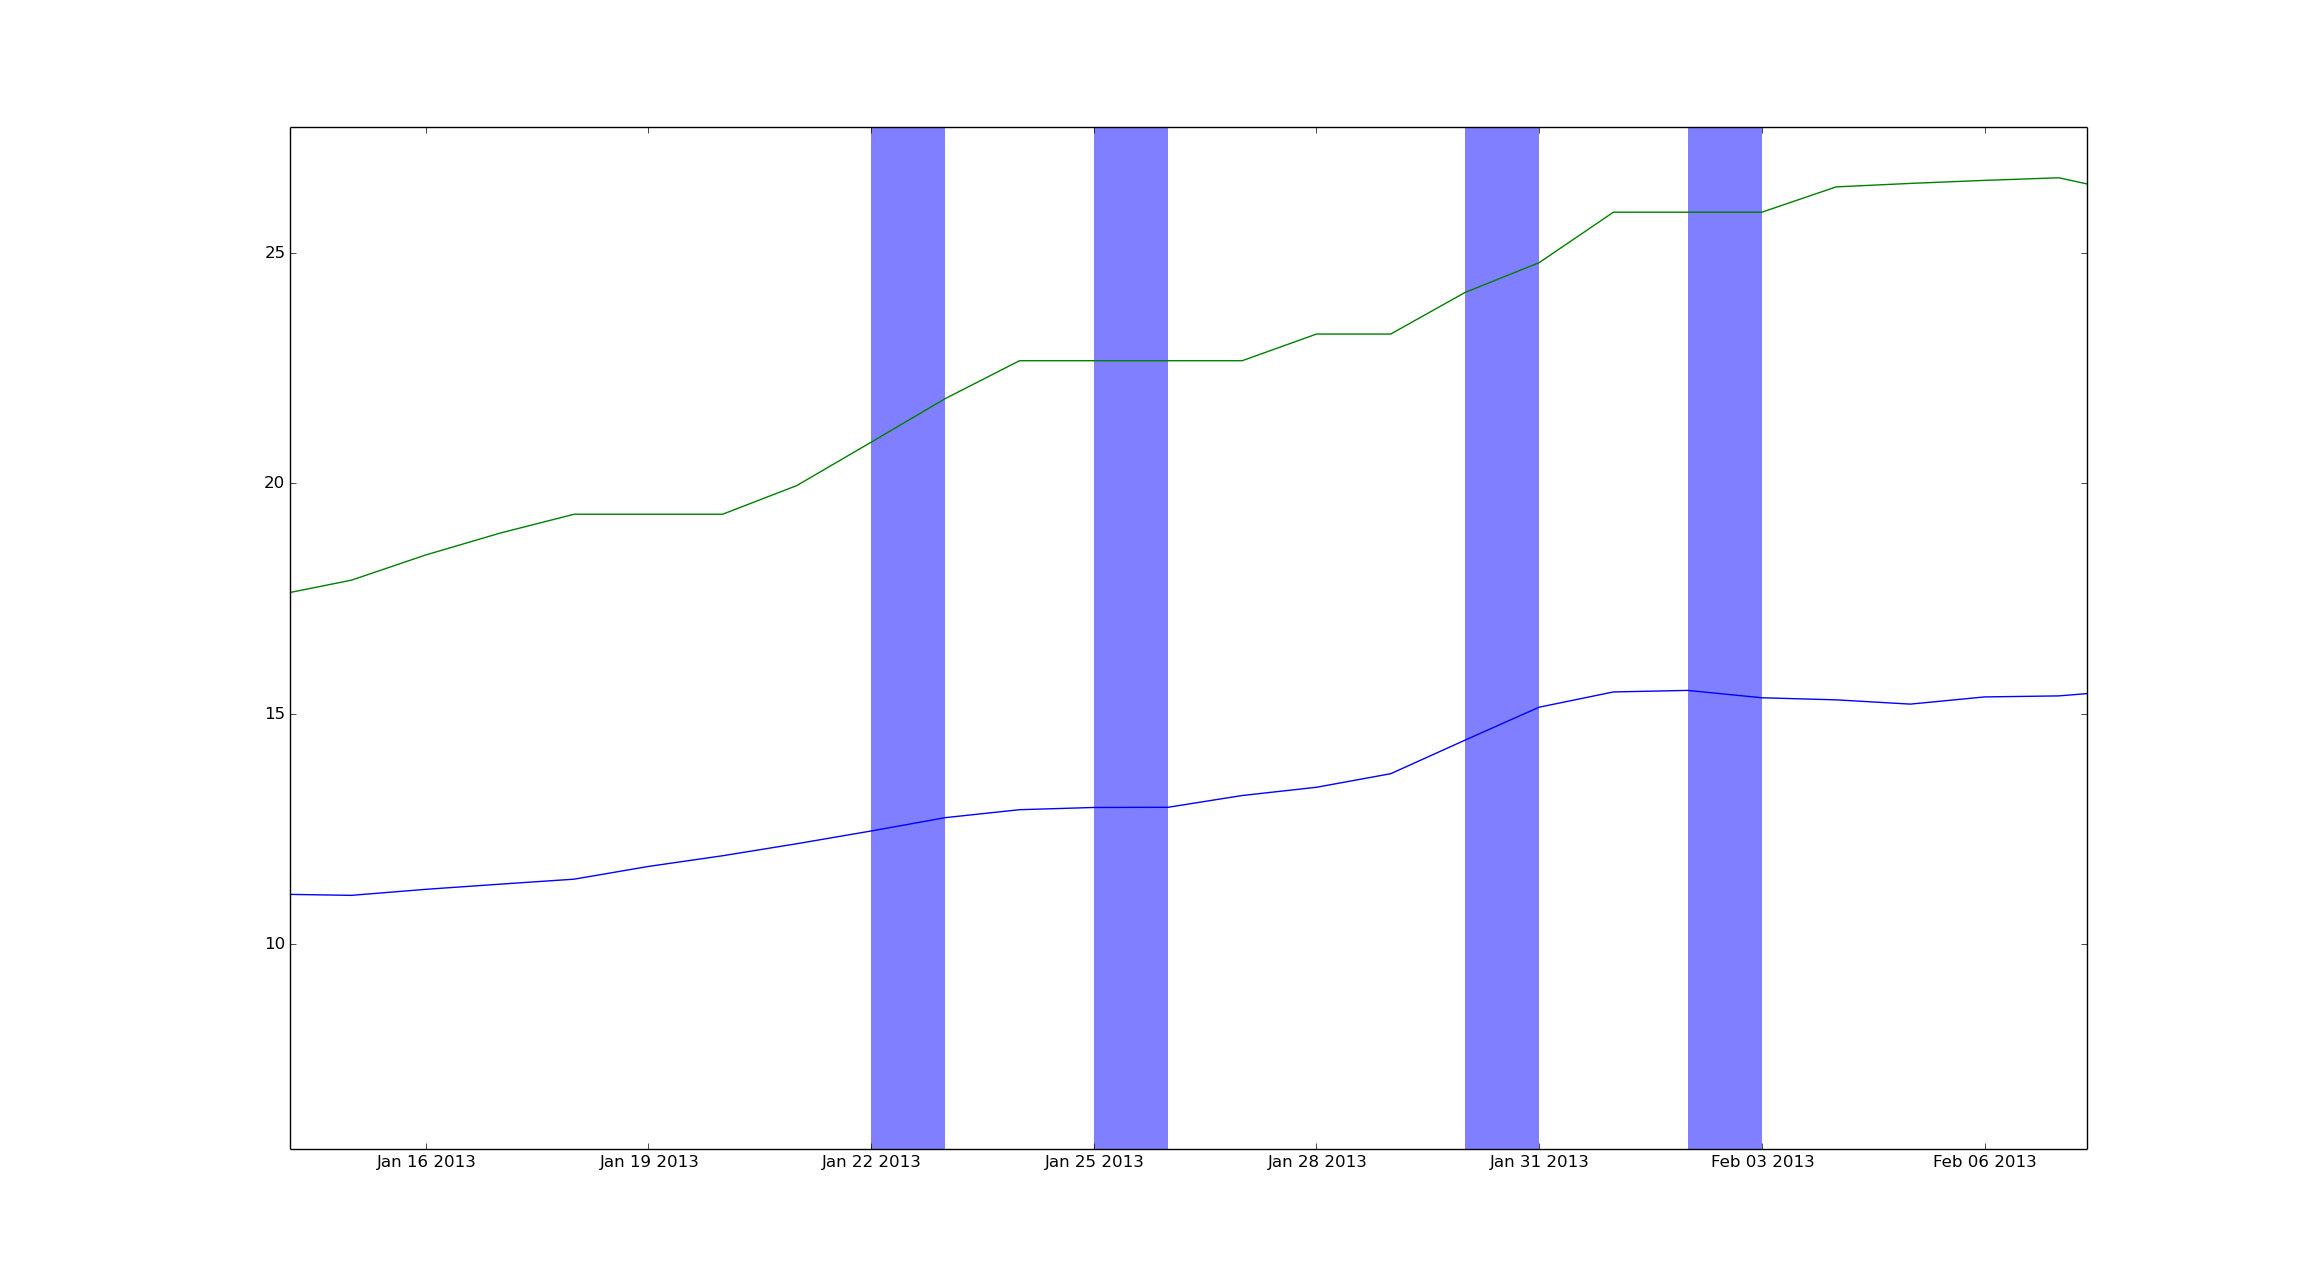
\includegraphics[width=0.8\textwidth]{graphs/12133.png}
		    	\caption{Slope Based Anomaly Detection (Green line - Retail Price, Blue Line - Wholesale Price)}
		    	\label{fig:12133}
			\end{figure}
			
			\item In some cases, original retail price was running less than average retail price for some time and then suddenly prices in the centre increased drastically. So such cases were reported as anomaly in this method, which is quite normal. Such cases were found in \textit{Analysis 1} for Nov 2011, Feb Mar 2012 and Dec 2014. (See Figure \ref{fig:12114})
			
			\begin{figure}[H]
		    	\centering
  		    	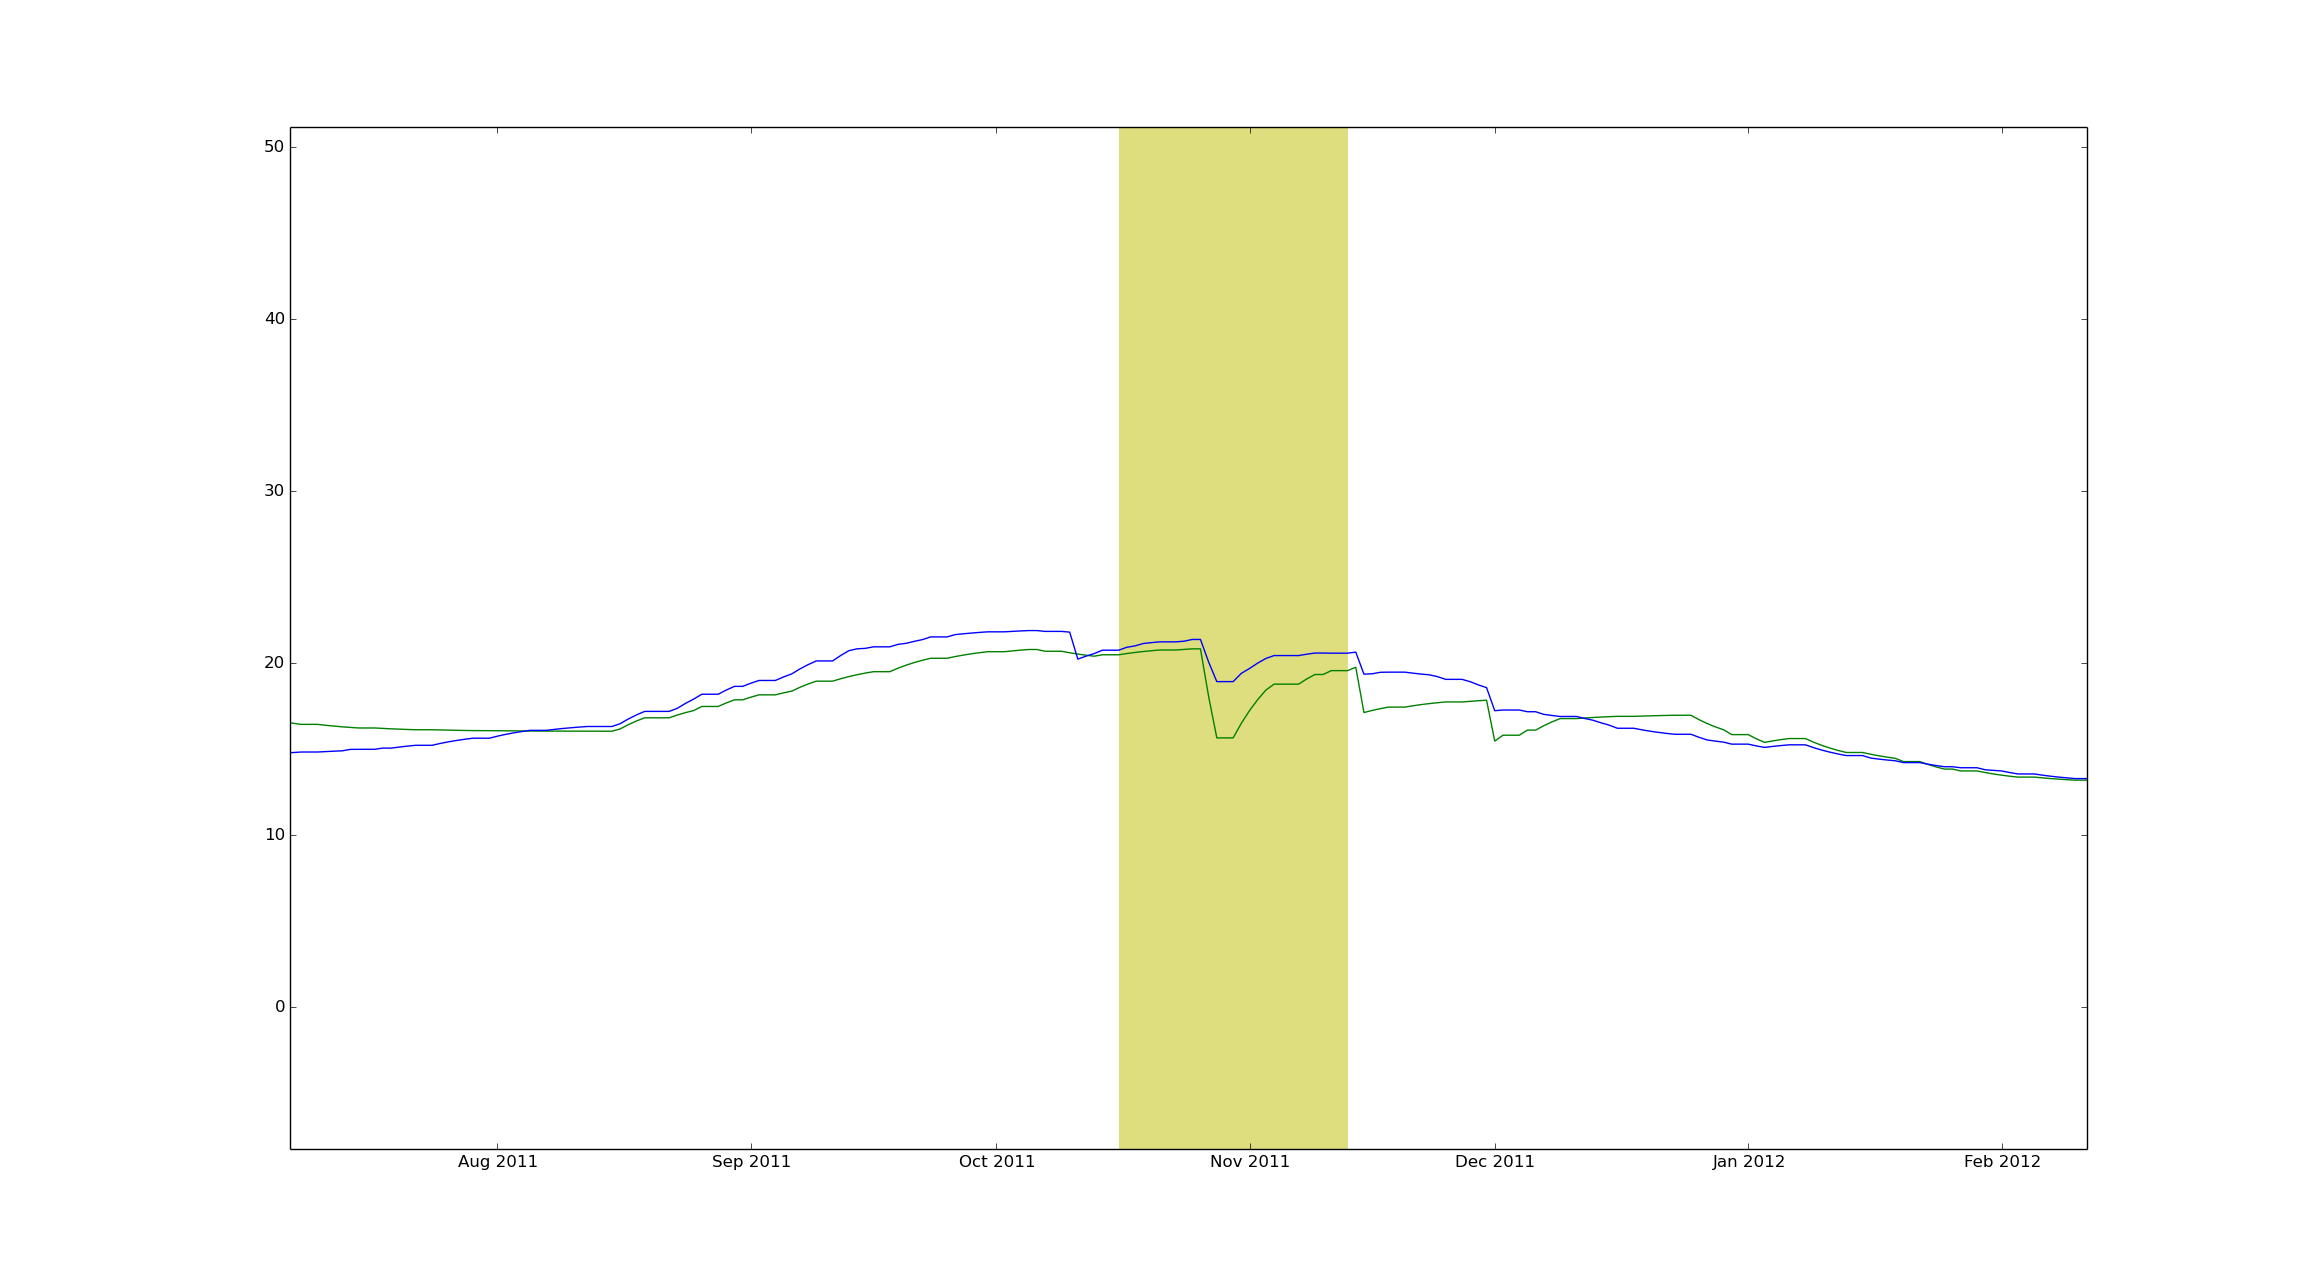
\includegraphics[width=0.8\textwidth]{graphs/12114.png}
		    	\caption{Slope Based Anomaly Detection (Green line - Centre Retail Price, Blue Line - Average Retail Price)}
		    	\label{fig:12114}
			\end{figure}			
			
			\item In some cases, tenure reported as anomaly is quite large, because situations were abnormal for long time. But is not necessary that news articles should be present for such a large tenure and anomaly reported was justifiable. For\textit{ Analysis 1}, such tenure was reported for March end to May start 2014.  (See Figure \ref{fig:12115})
			
			\begin{figure}[H]
		    	\centering
  		    	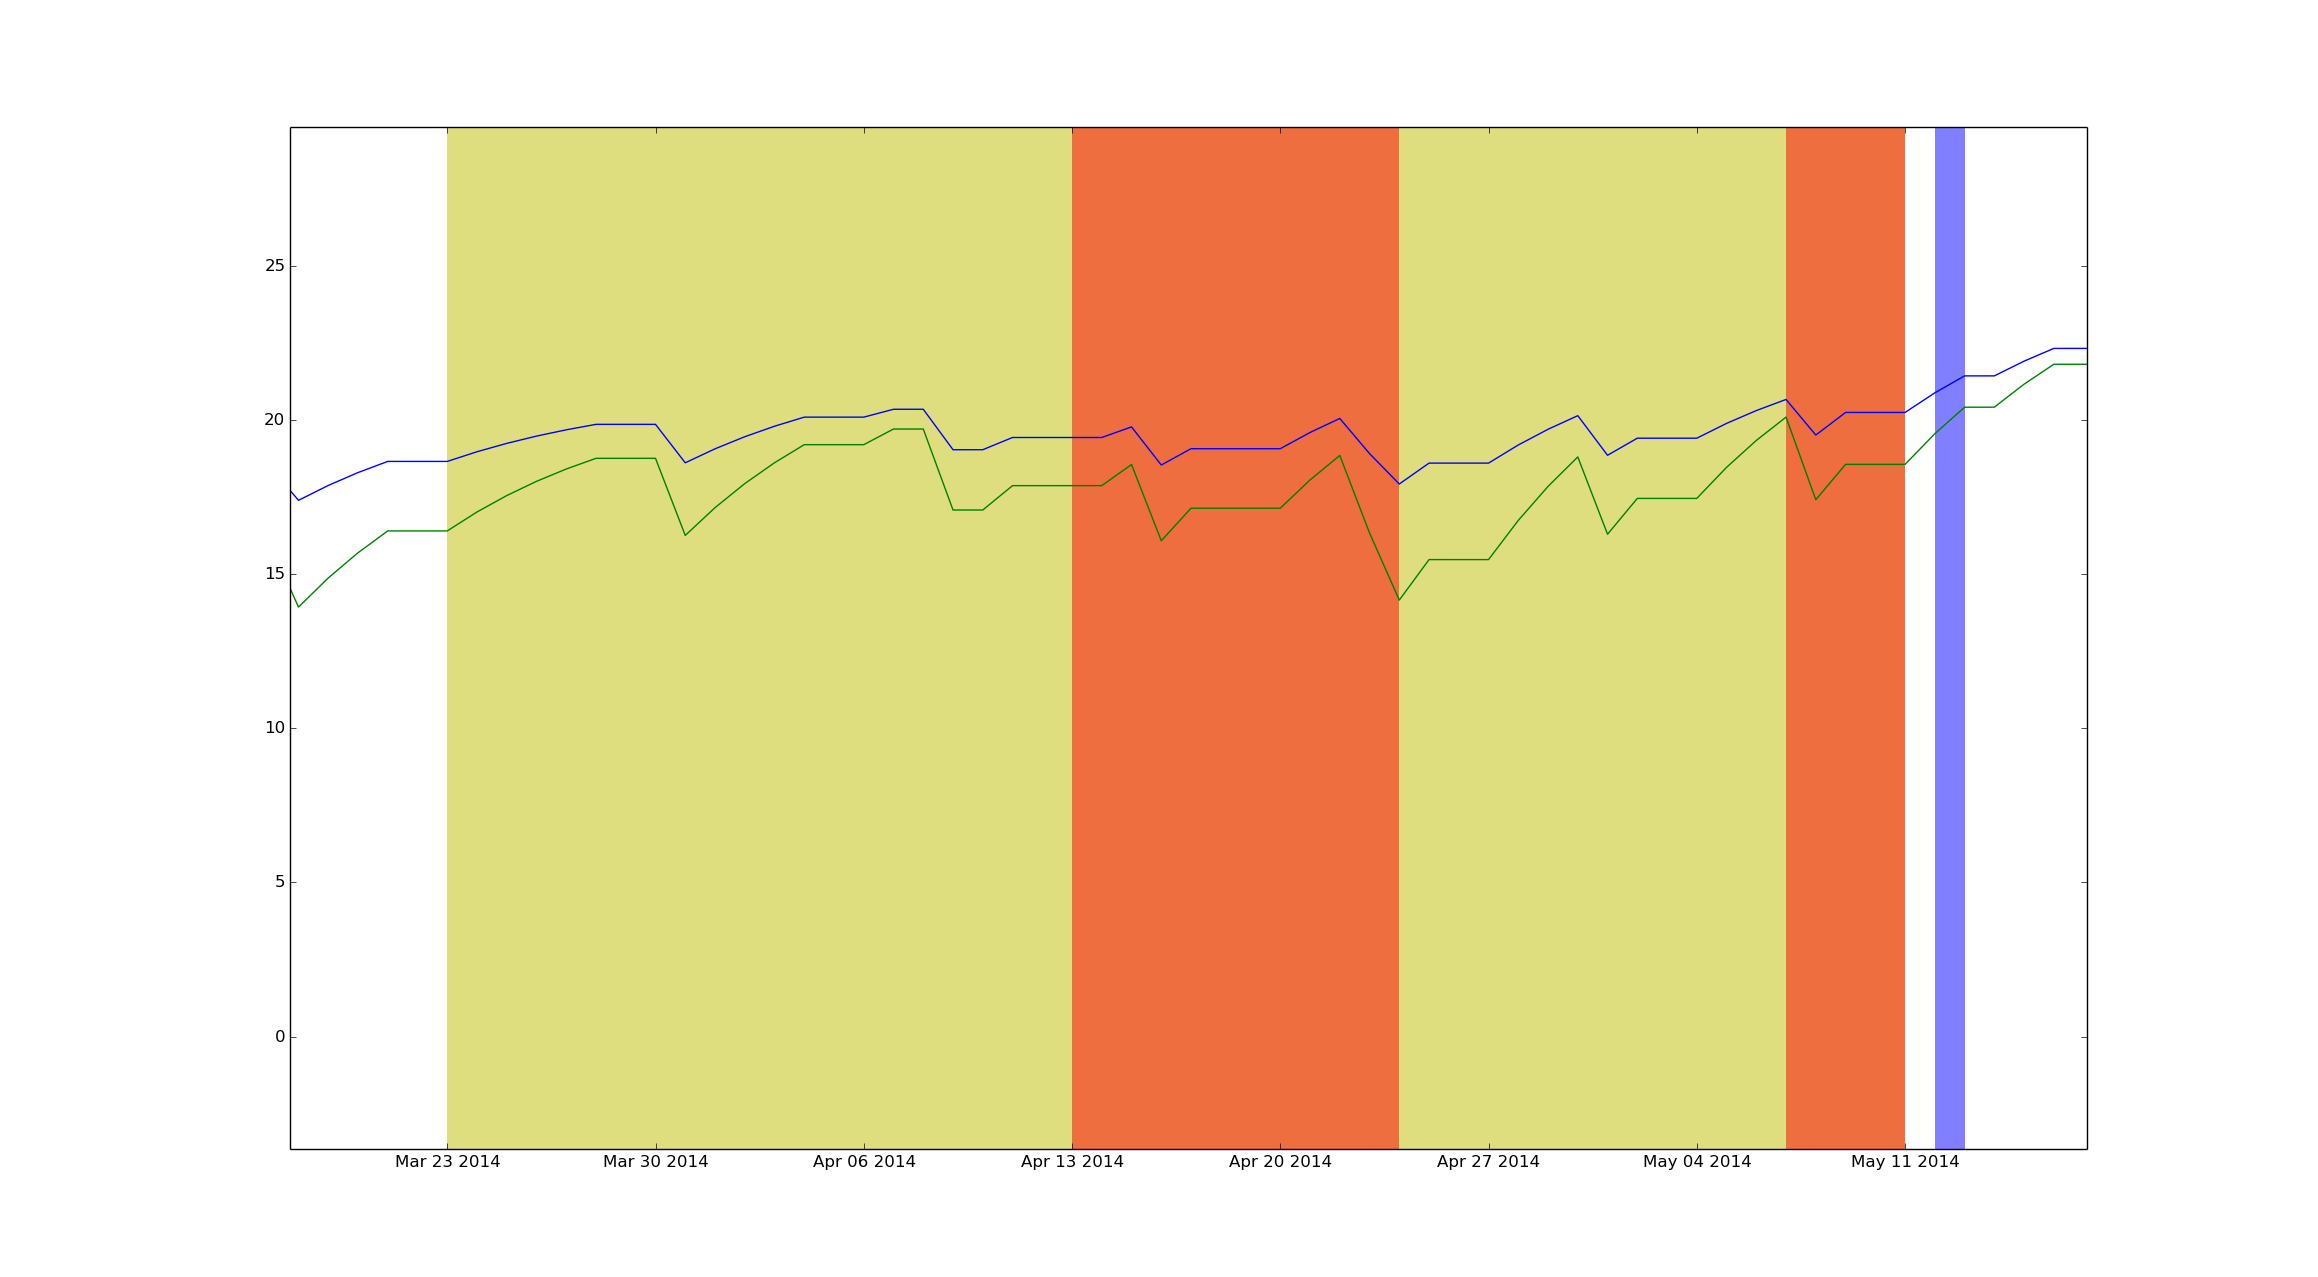
\includegraphics[width=0.8\textwidth]{graphs/12115.png}
		    	\caption{Slope Based Anomaly Detection (Green line - Centre Retail Price, Blue Line - Average Retail Price)}
		    	\label{fig:12115}
			\end{figure}			
			
			\item In \textit{Analysis 1} for June 2014, method has reported tenure upto mid June when prices started increasing but it remained high and due to that some news articles are present around June 21. We have missed because at that time relative slope value became normal. But since prices were high, it was covered by news articles. (See Figure \ref{fig:12116})
			
			\begin{figure}[H]
		    	\centering
  		    	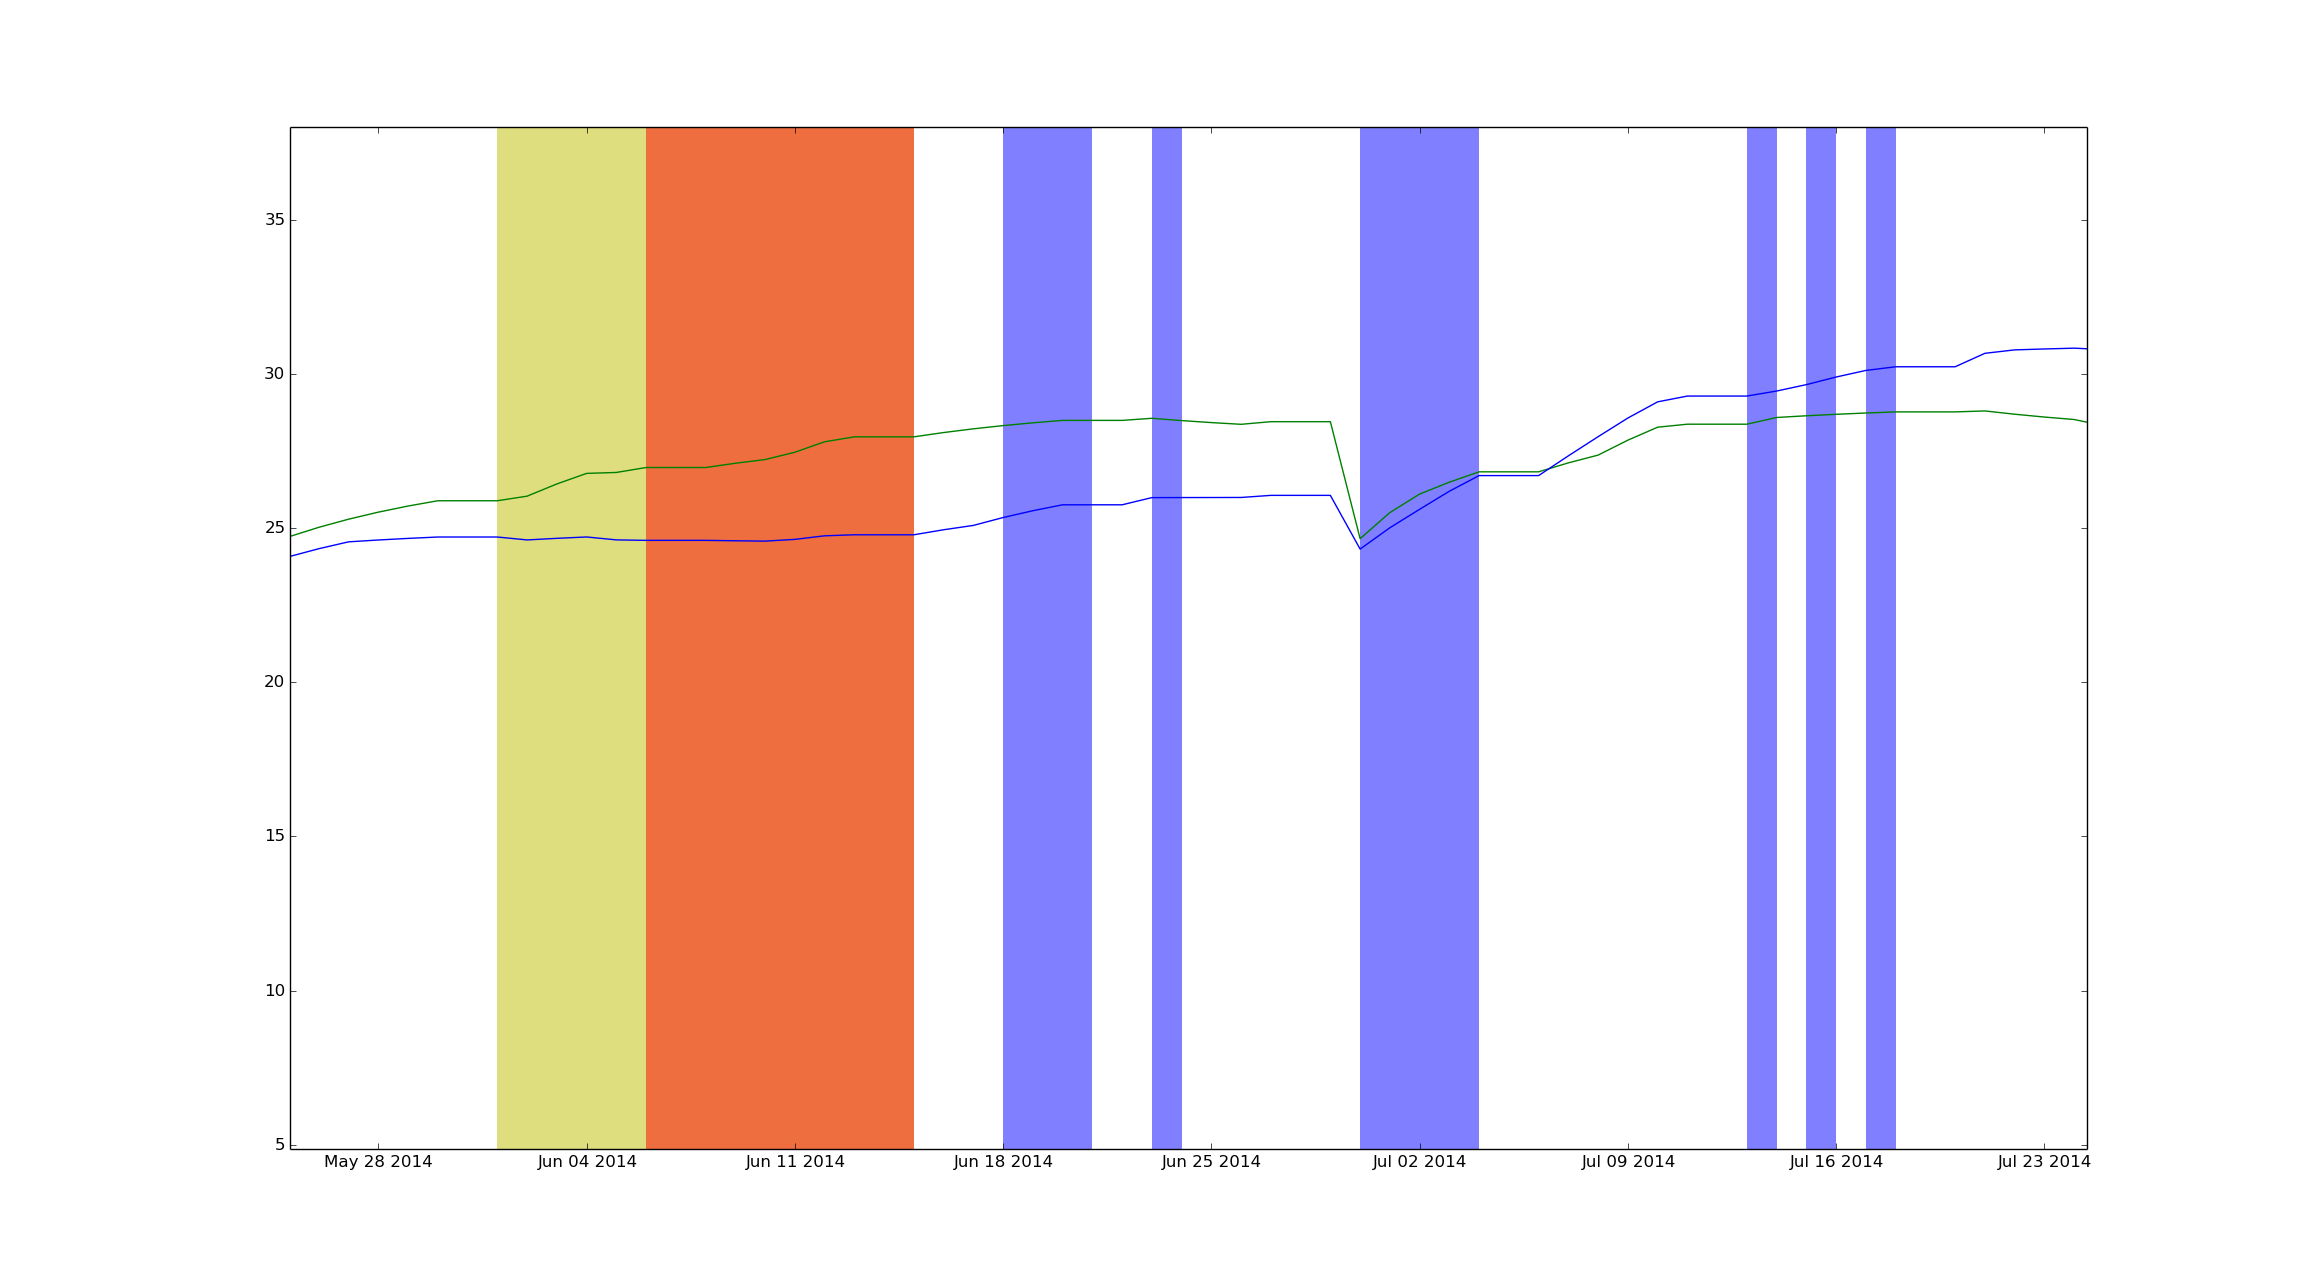
\includegraphics[width=0.8\textwidth]{graphs/12116.png}
		    	\caption{Slope Based Anomaly Detection (Green line - Centre Retail Price, Blue Line - Average Retail Price)}
		    	\label{fig:12116}
			\end{figure}			
			
			
			\item There exist some cases in \textit{Analysis 3} where retail price were decreasing but wholesale price kept on increasing, this created negative slope value, whereas in this scenario, we were looking for only positive slopes and that's why this method missed it. Such periods were in July Aug Sept 2013, Nov Dec 2013. (See Figure \ref{fig:12134})
			
			\begin{figure}[H]
		    	\centering
  		    	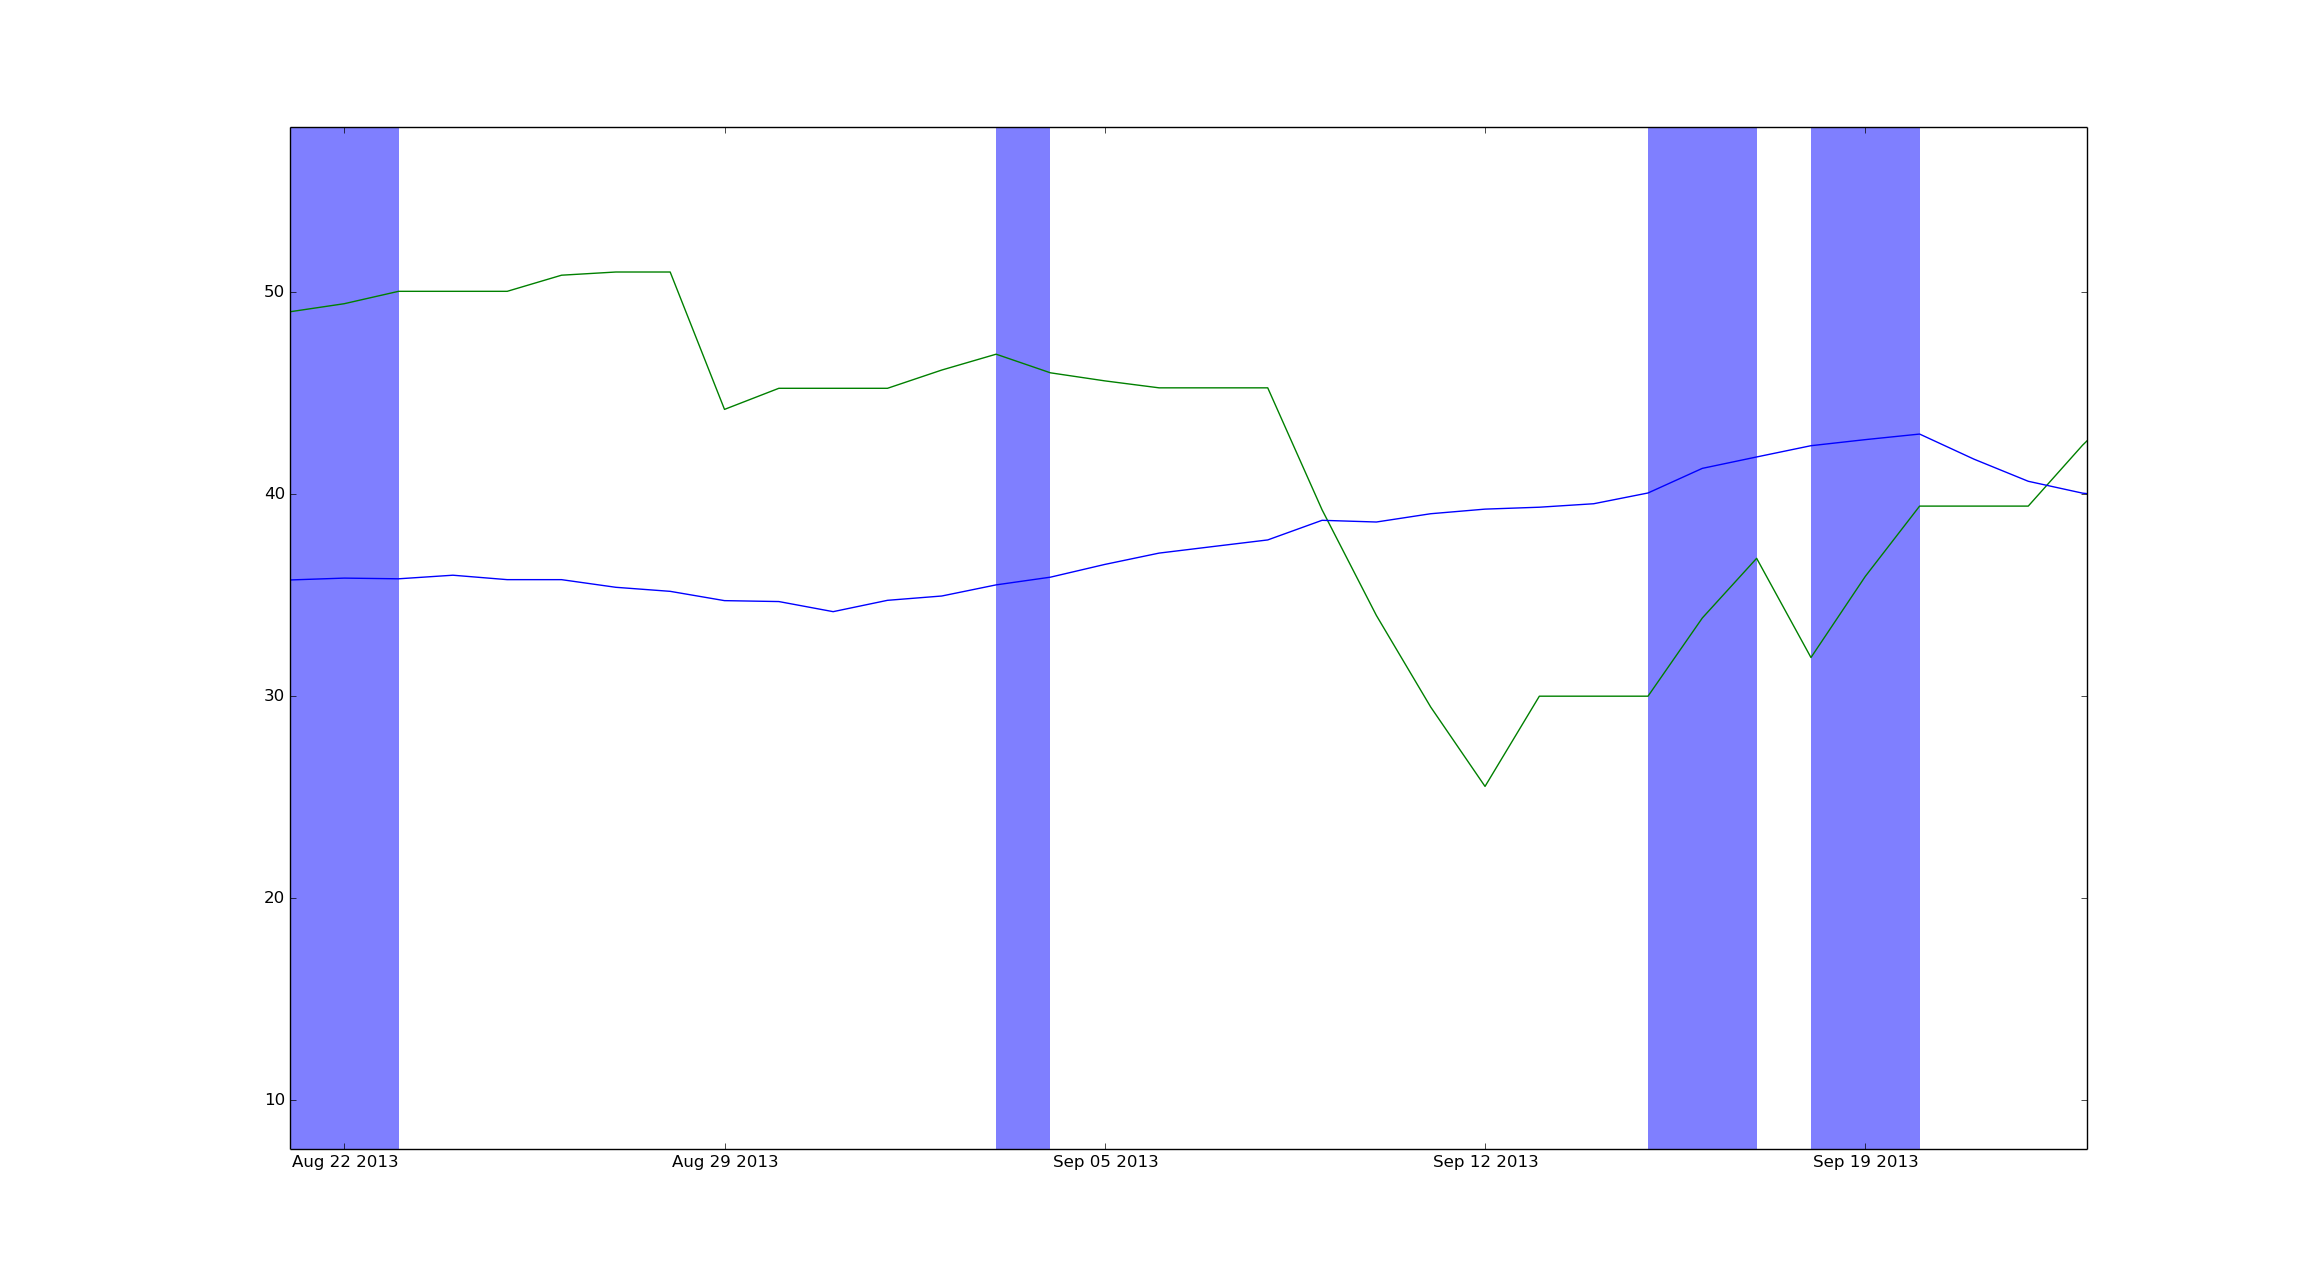
\includegraphics[width=0.8\textwidth]{graphs/12134.png}
		    	\caption{Slope Based Anomaly Detection (Green line - Retail Price, Blue Line - Wholesale Price)}
		    	\label{fig:12134}
			\end{figure}			
			
		\end{itemize}
		
		
		Now we present few observation for Analysis 2 and 4.
		
		\begin{itemize}
			\item If change in retail price or change in wholesale price is more as compared to change in arrival (prices went too high, even for small drop in arrival), then it is reported as anomaly by this method.\\
			
			Following tenures are some cases reported by this method:
			\begin{itemize}
				\item \textit{Analysis 2}: Oct Dec 2010, May Jun 2013 (See Figure \ref{fig:12121})
				\item \textit{Analysis 4}: Sept Oct Nov 2010, Jun 2013, Jun 2015 (See Figure \ref{fig:12141})
			\end{itemize}	
			
			\begin{figure}[H]
		    	\centering
  		    	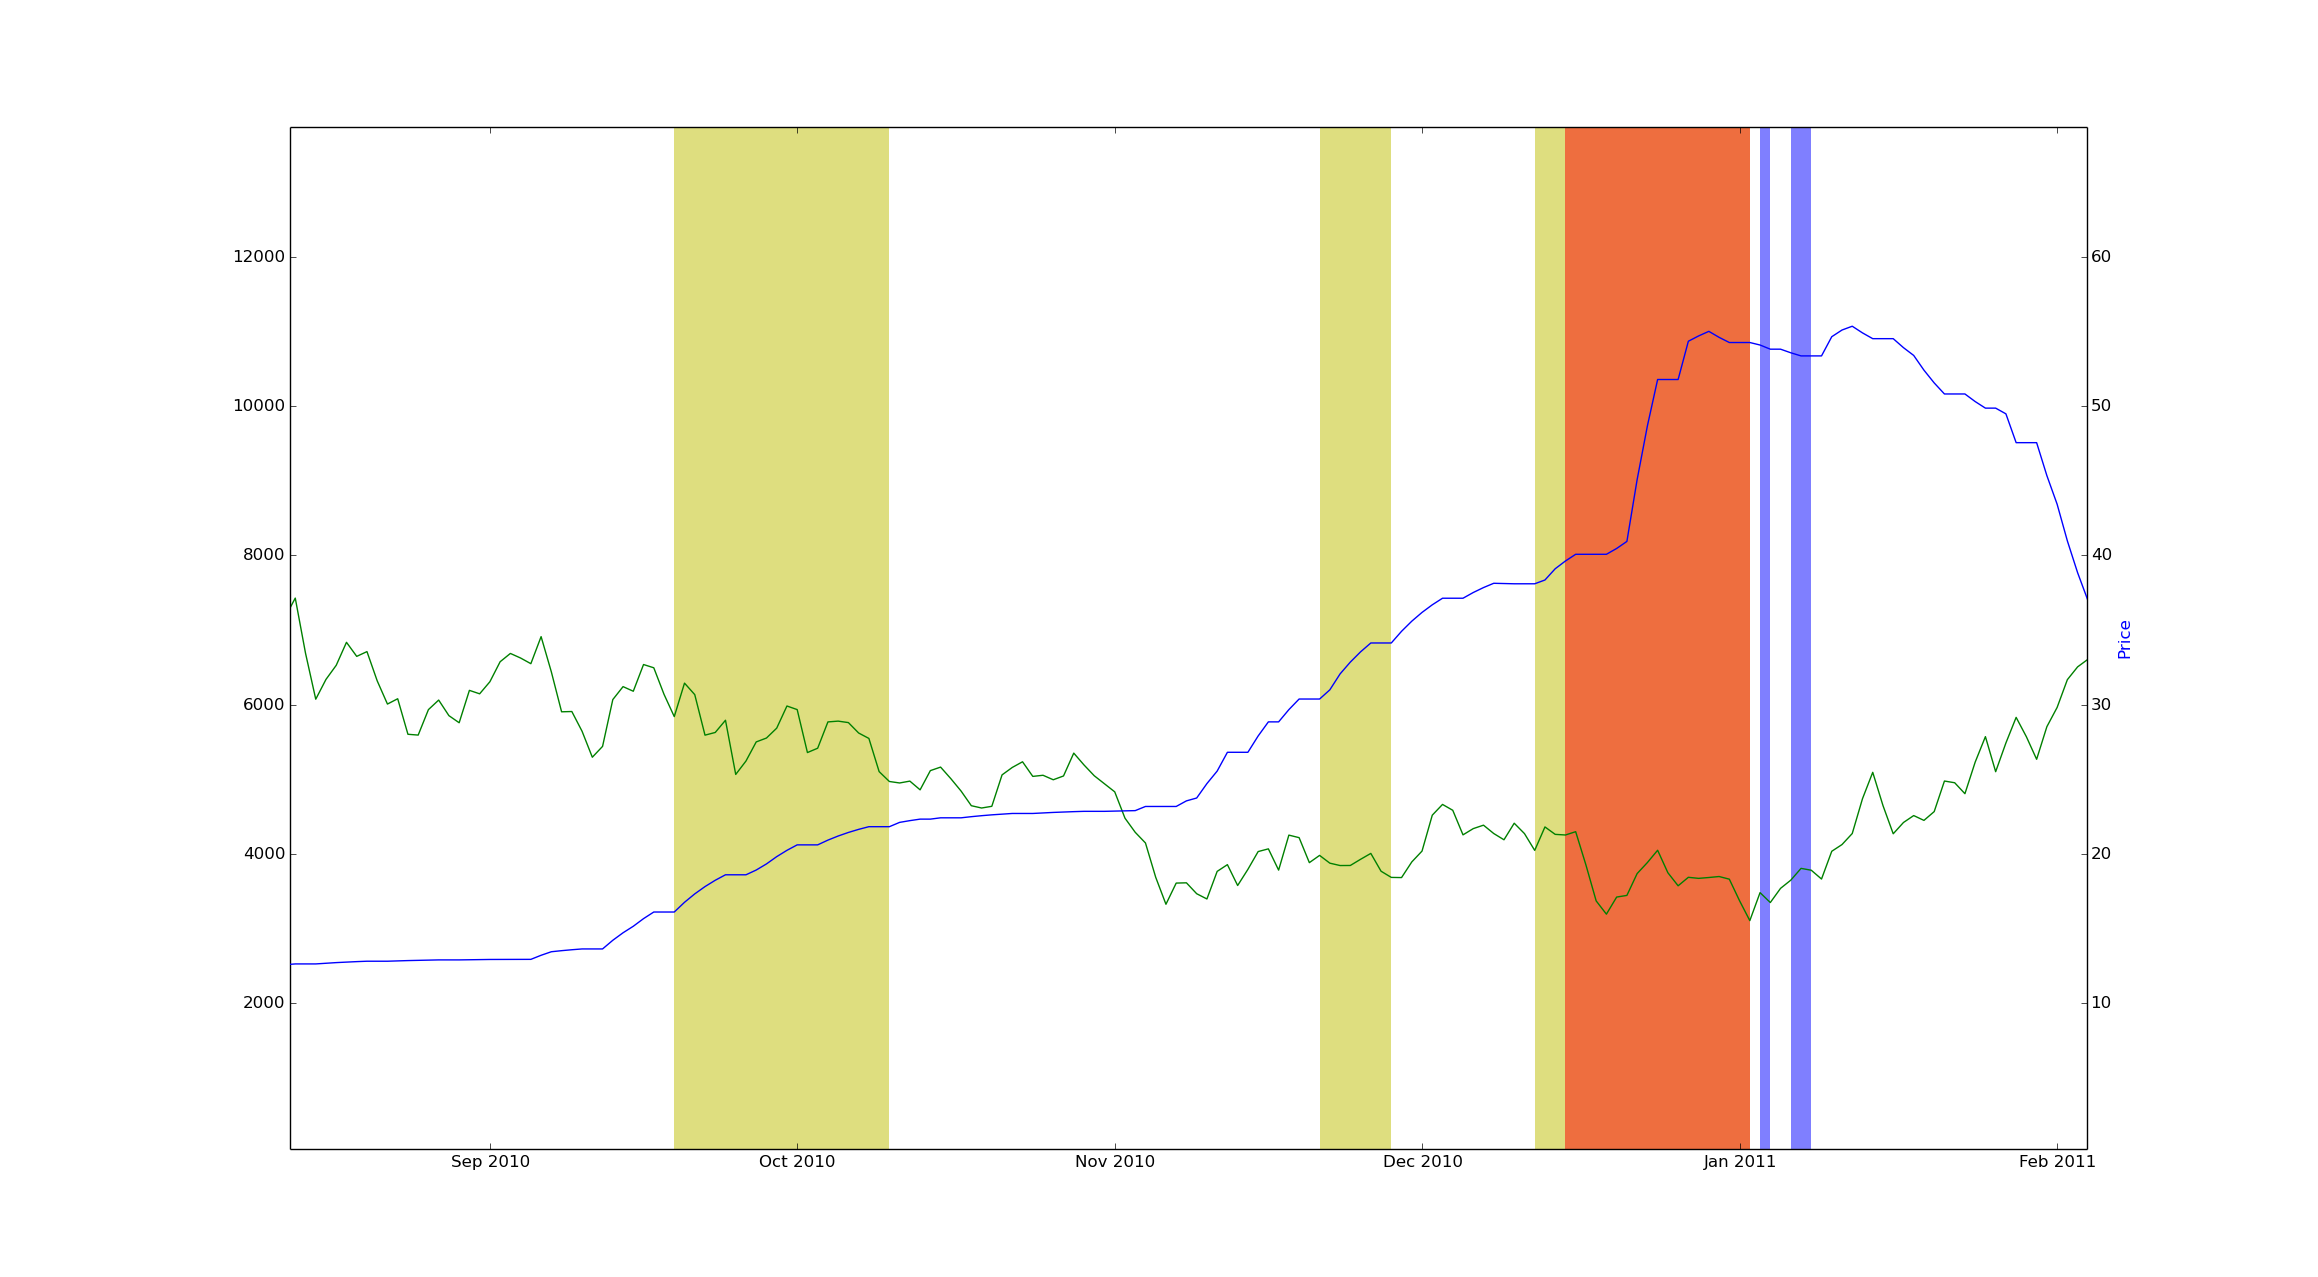
\includegraphics[width=0.8\textwidth]{graphs/12121.png}
		    	\caption{Slope Based Anomaly Detection (Green line - Arrival Data of Onion, Blue Line - Retail Price)}
		    	\label{fig:12121}
			\end{figure}
			
			\begin{figure}[H]
		    	\centering
  		    	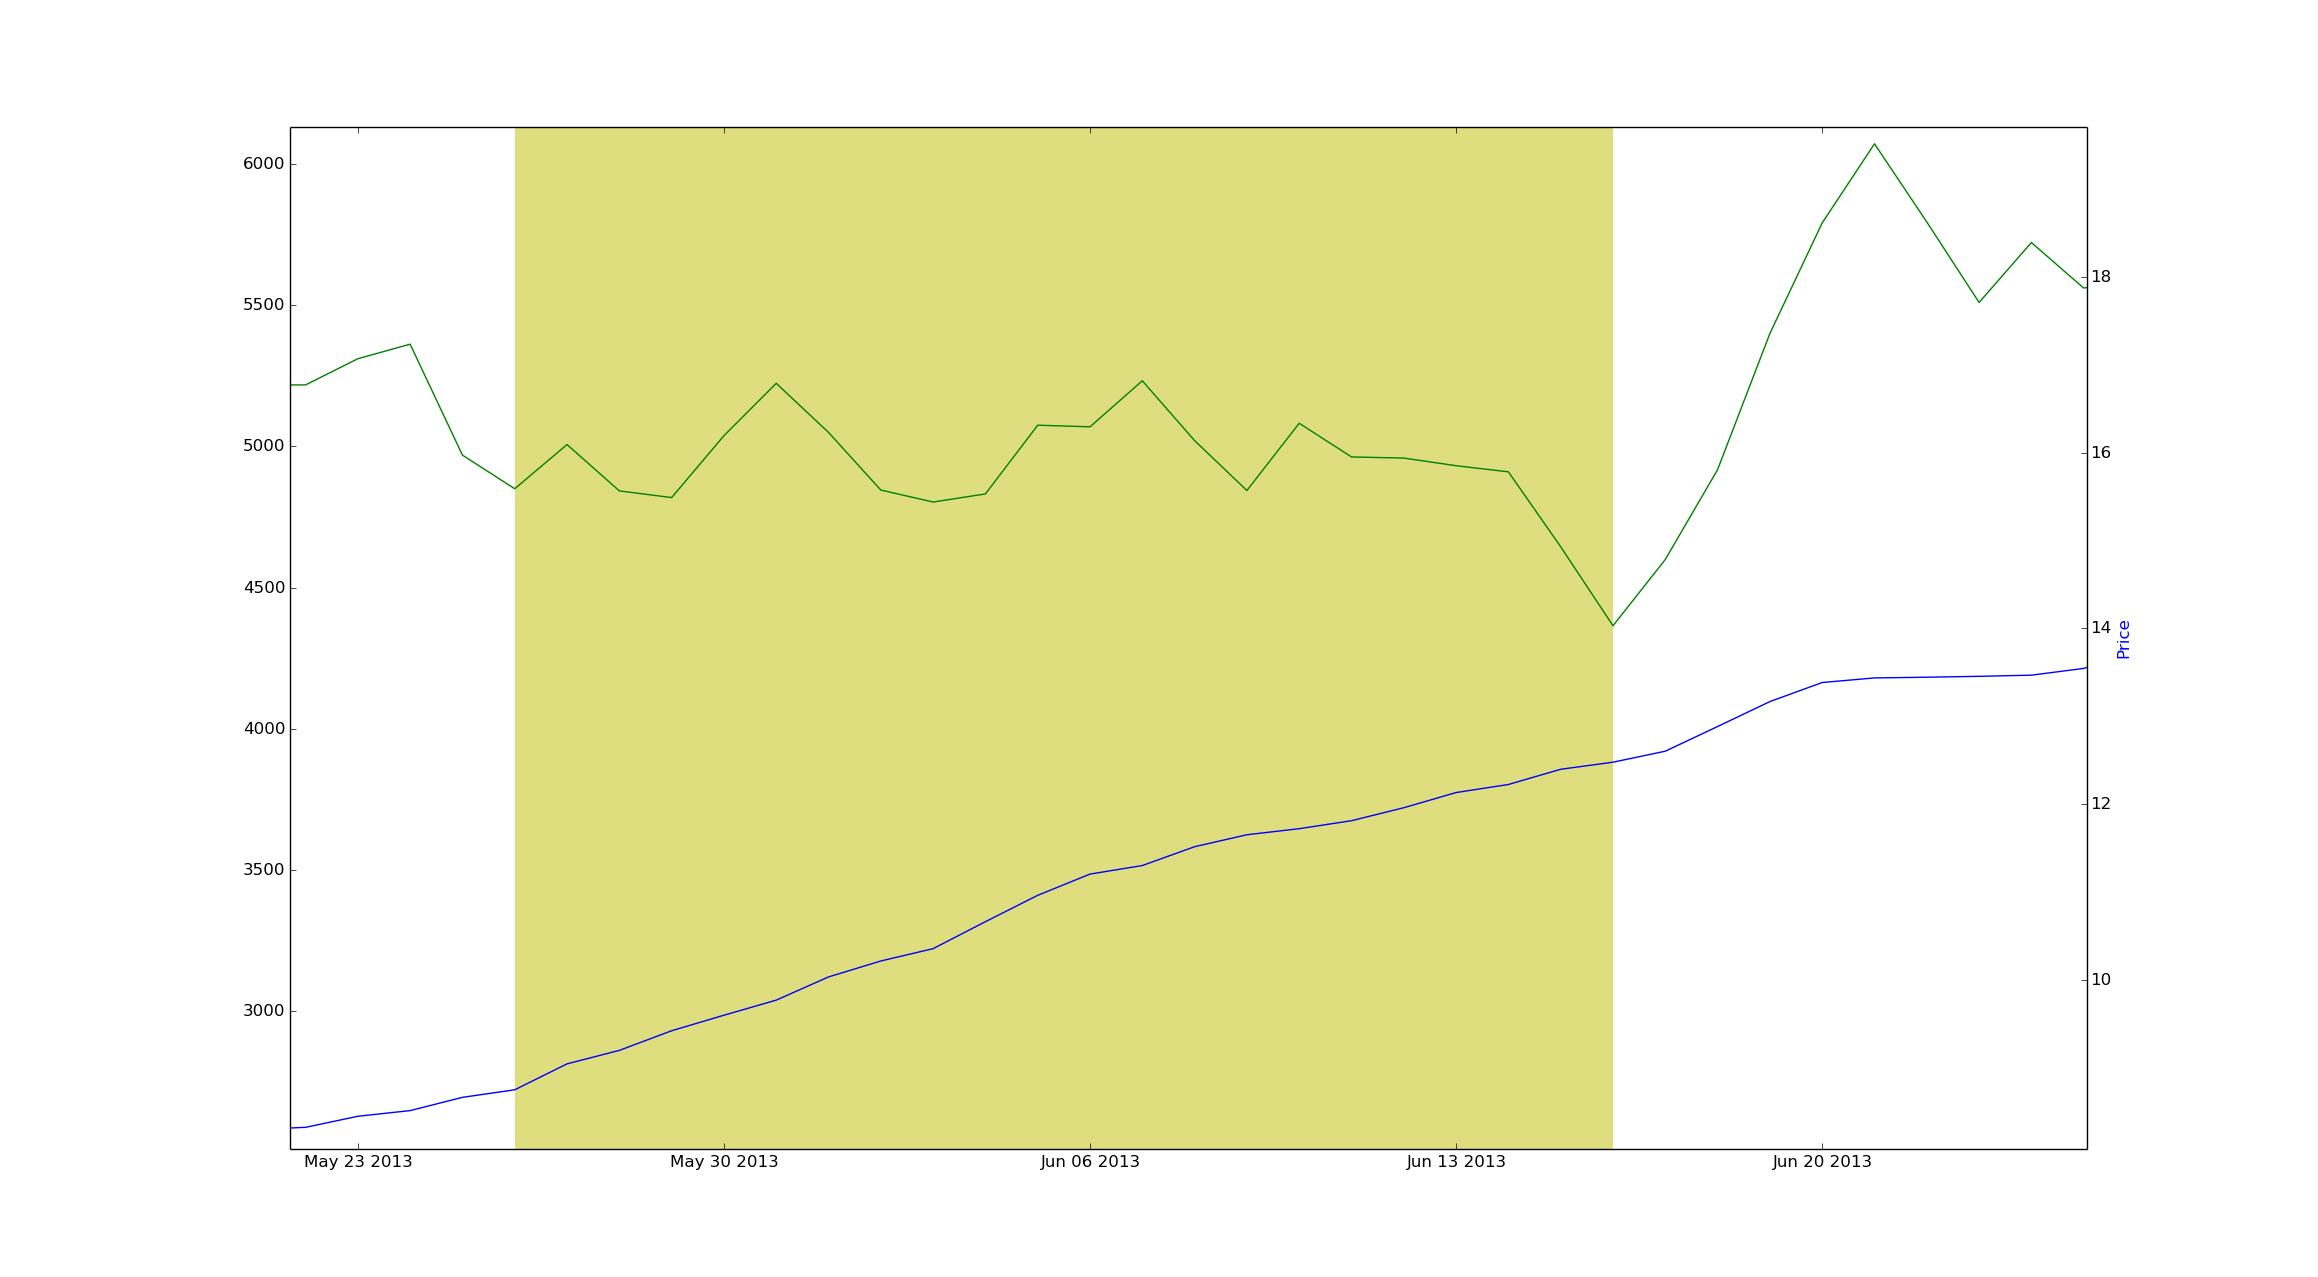
\includegraphics[width=0.8\textwidth]{graphs/12141.png}
		    	\caption{Slope Based Anomaly Detection (Green line - Arrival Data of Onion, Blue Line - Wholesale Price)}
		    	\label{fig:12141}
			\end{figure}
			
			\item But in above described scenario, when change in price is high, but prices are decreasing and when arrival is increasing, and if drop in price is too high, then also it will be reported as anomaly.	So this is limitation of this method and reports false positives in this case.\\
			Following tenures are some cases reported by this method:
			
			\begin{itemize}
				\item \textit{Analysis 2}: Feb Mar 2011, Jan Feb 2014 (See Figure \ref{fig:12122})
				\item \textit{Analysis 4}: Oct Dec 2011, Jan 2014, Mar 2011 (See Figure \ref{fig:12142})
			\end{itemize}
			
			\begin{figure}[H]
		    	\centering
  		    	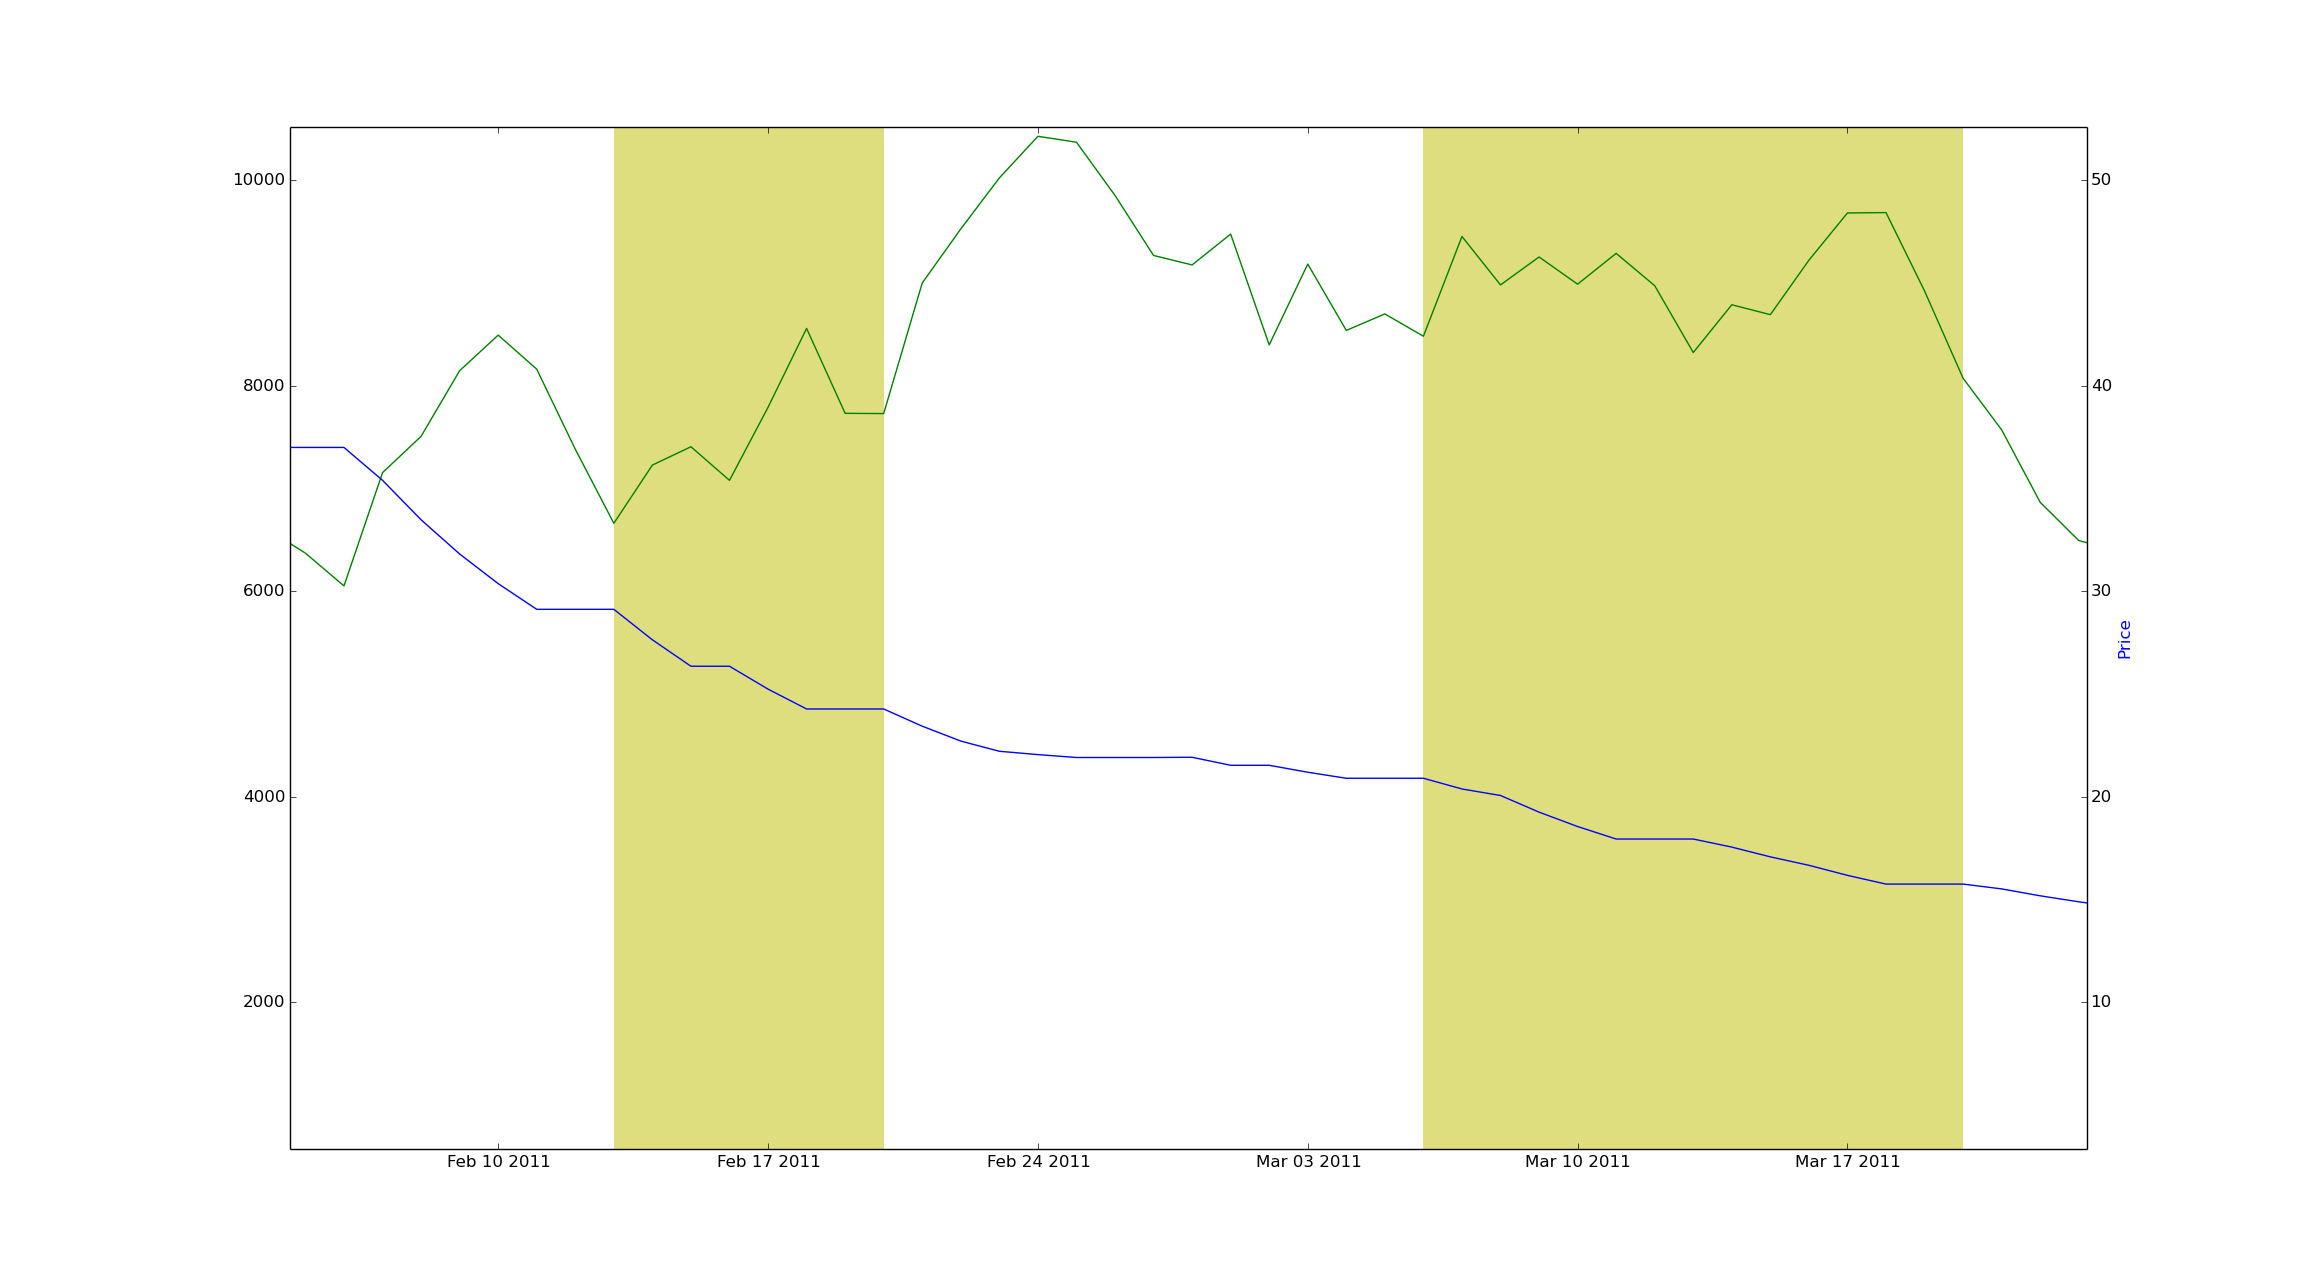
\includegraphics[width=0.8\textwidth]{graphs/12122.png}
		    	\caption{Slope Based Anomaly Detection (Green line - Arrival Data of Onion, Blue Line - Retail Price)}
		    	\label{fig:12122}
			\end{figure}
			
			\begin{figure}[H]
		    	\centering
  		    	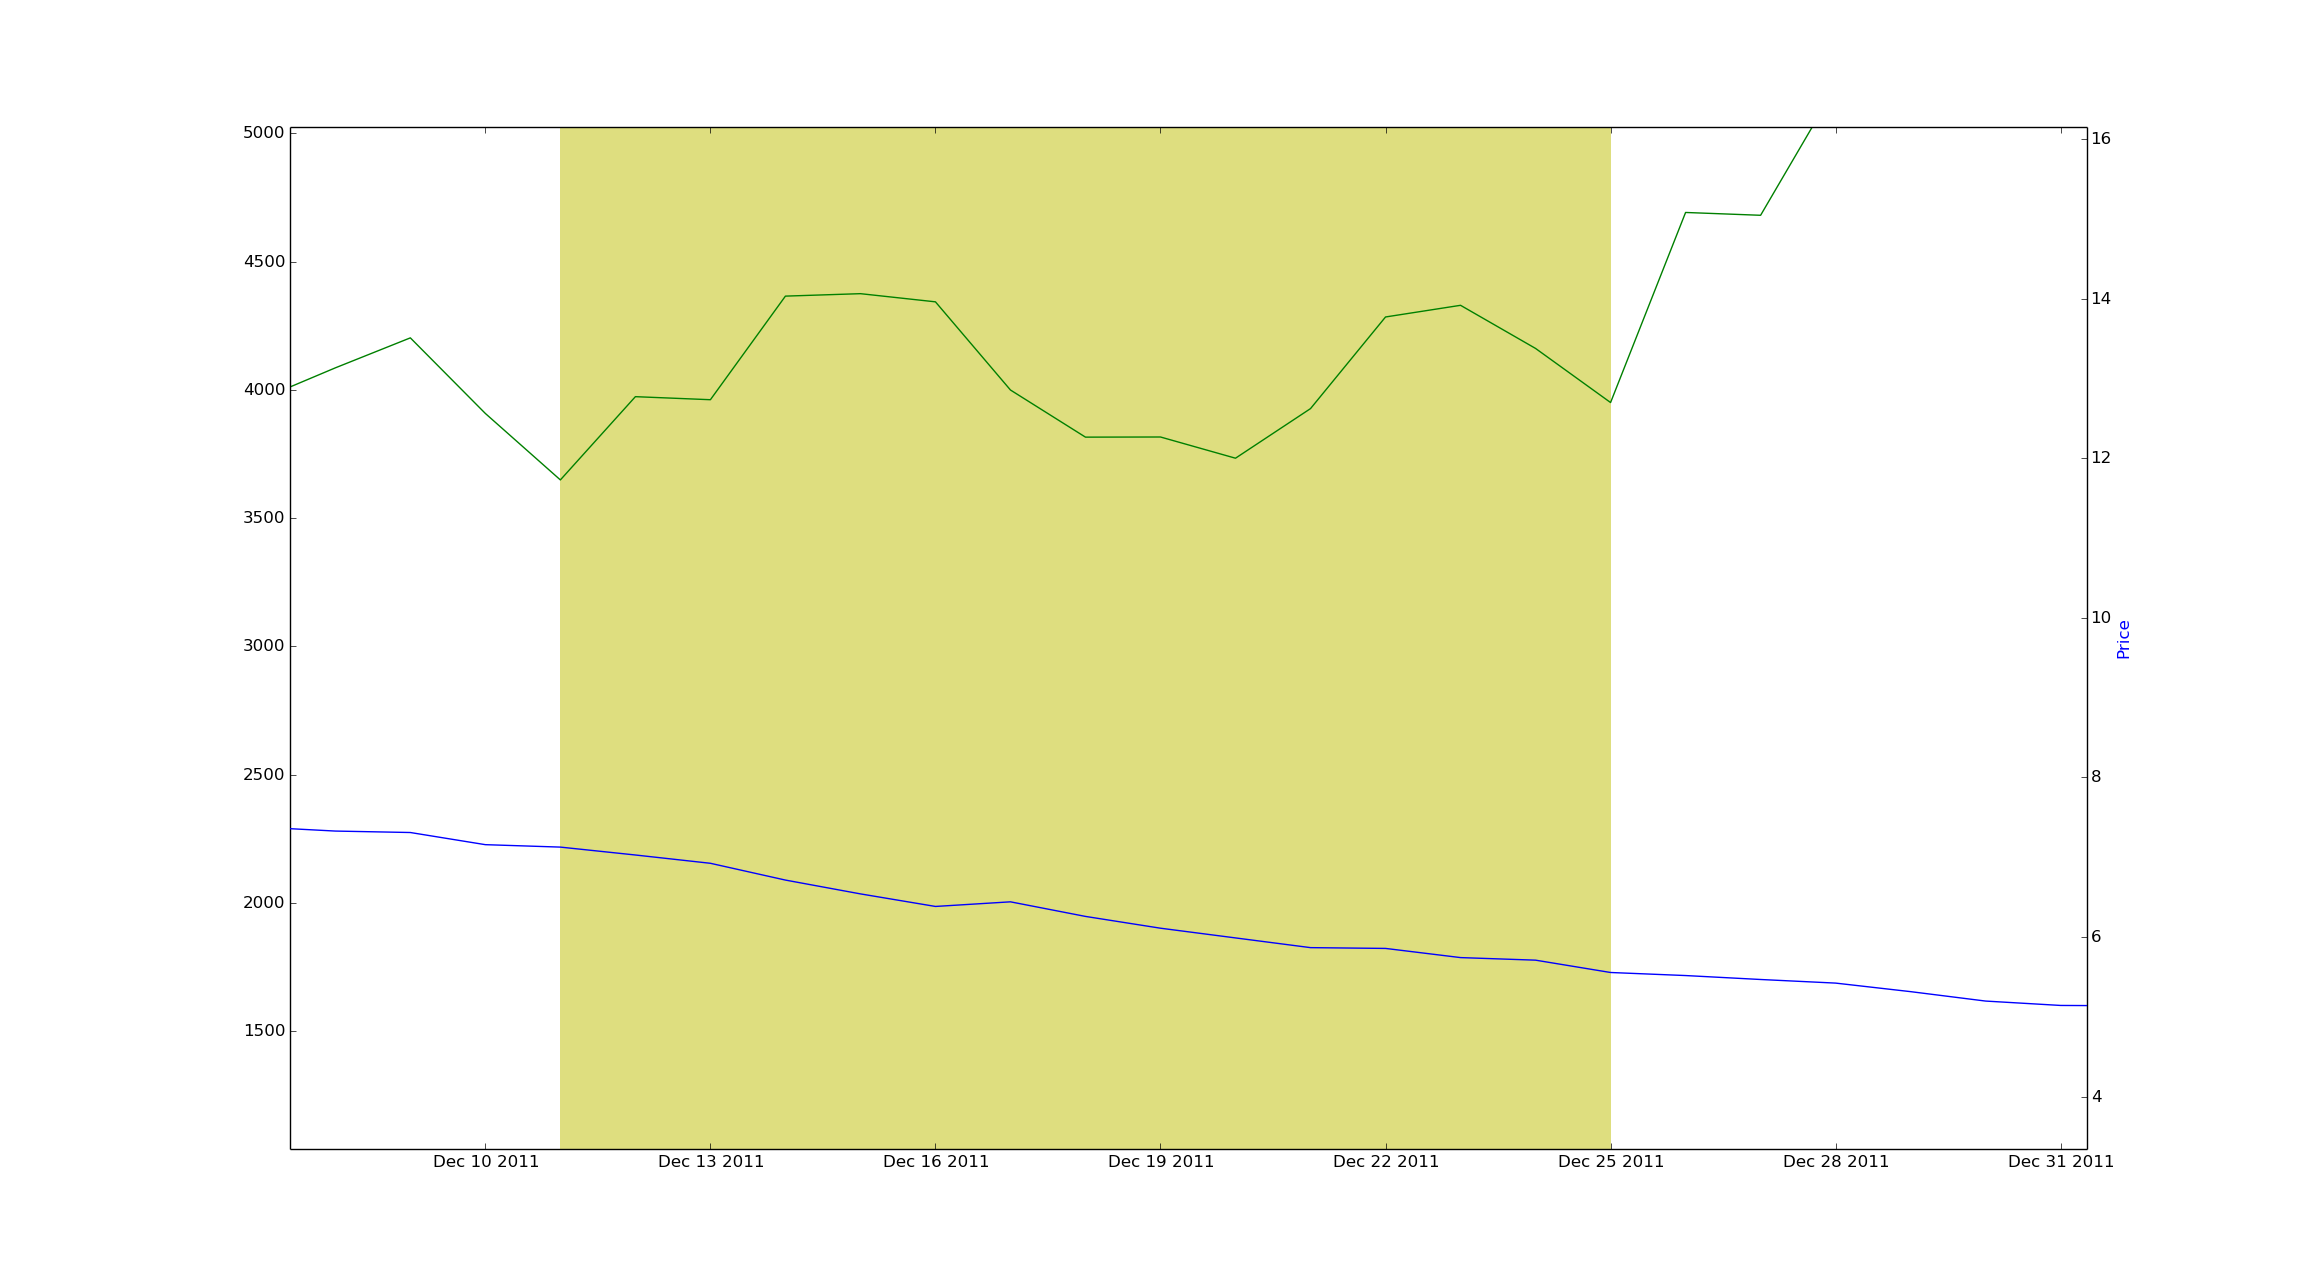
\includegraphics[width=0.8\textwidth]{graphs/12142.png}
		    	\caption{Slope Based Anomaly Detection (Green line - Arrival Data of Onion, Blue Line - Wholesale Price)}
		    	\label{fig:12142}
			\end{figure}
			
			\item One more limitation of this method is when arrival is increasing but along with that retail or wholesale price is also increasing. This will result into a positive slope and in this scenario we are only looking for negative slope and that's why, this will not be reported as anomaly and news articles corresponding to this tenure will not be matched by results of this method.\\		
			
			Following tenures are some cases reported by this method:
			\begin{itemize}
				\item \textit{Analysis 2}: Jan Feb July Nov 2013, June July 2014 (See Figure \ref{fig:12123})
				\item \textit{Analysis 4}: Jan Feb 2013, July 2014, June 2015 (See Figure \ref{fig:12143})
			\end{itemize}
			
			\begin{figure}[H]
		    	\centering
  		    	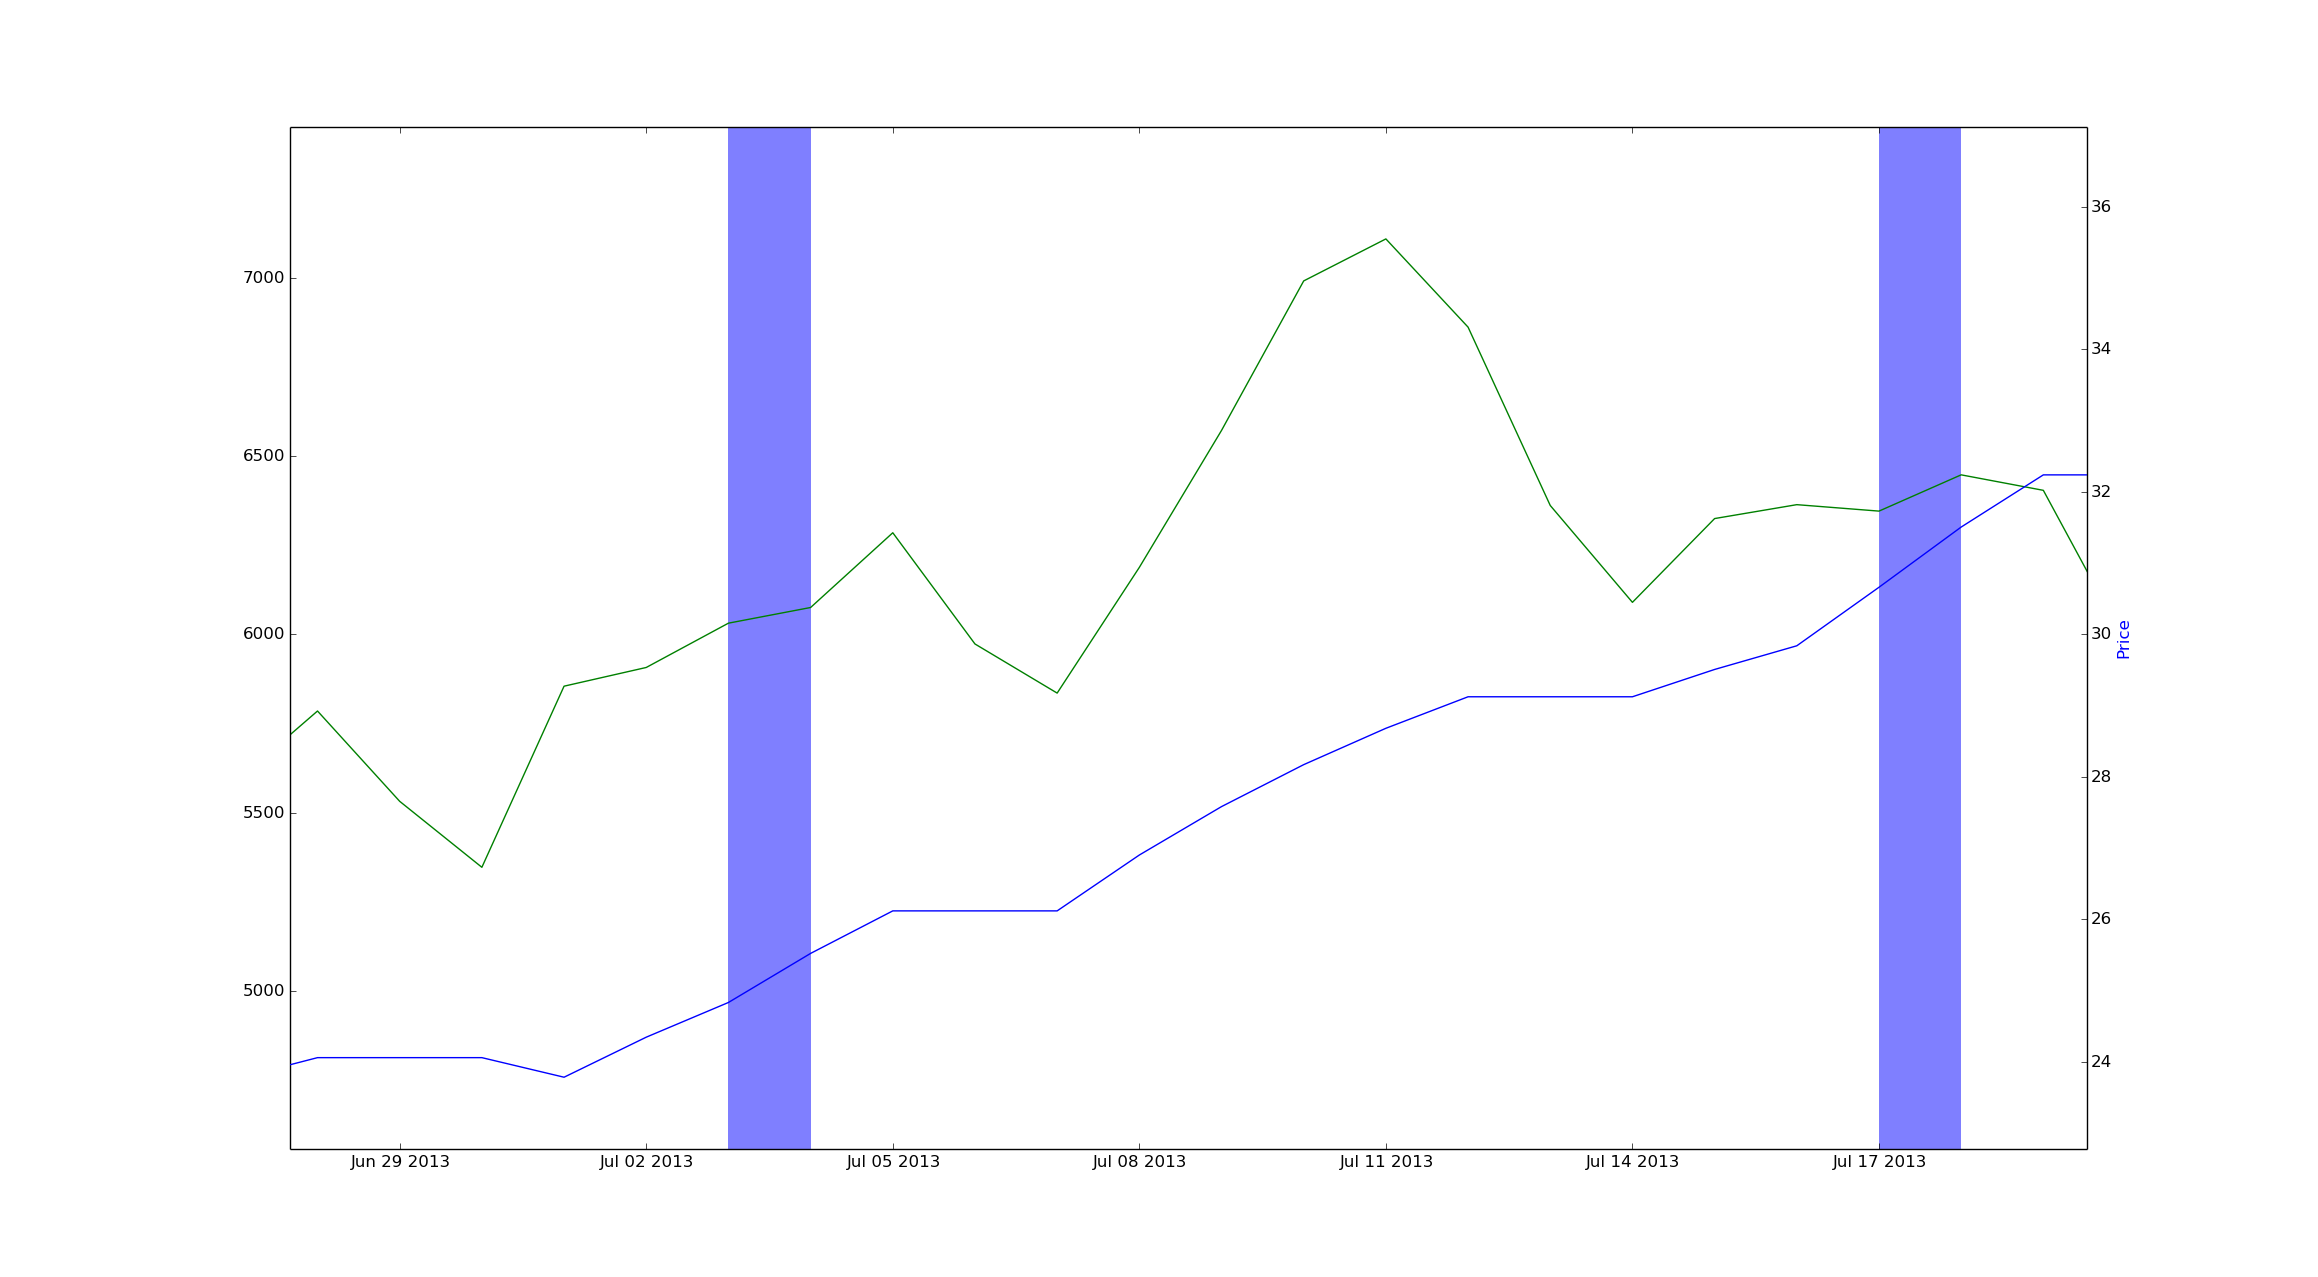
\includegraphics[width=0.8\textwidth]{graphs/12123.png}
		    	\caption{Slope Based Anomaly Detection (Green line - Arrival Data of Onion, Blue Line - Retail Price)}
		    	\label{fig:12123}
			\end{figure}
			
			\begin{figure}[H]
		    	\centering
  		    	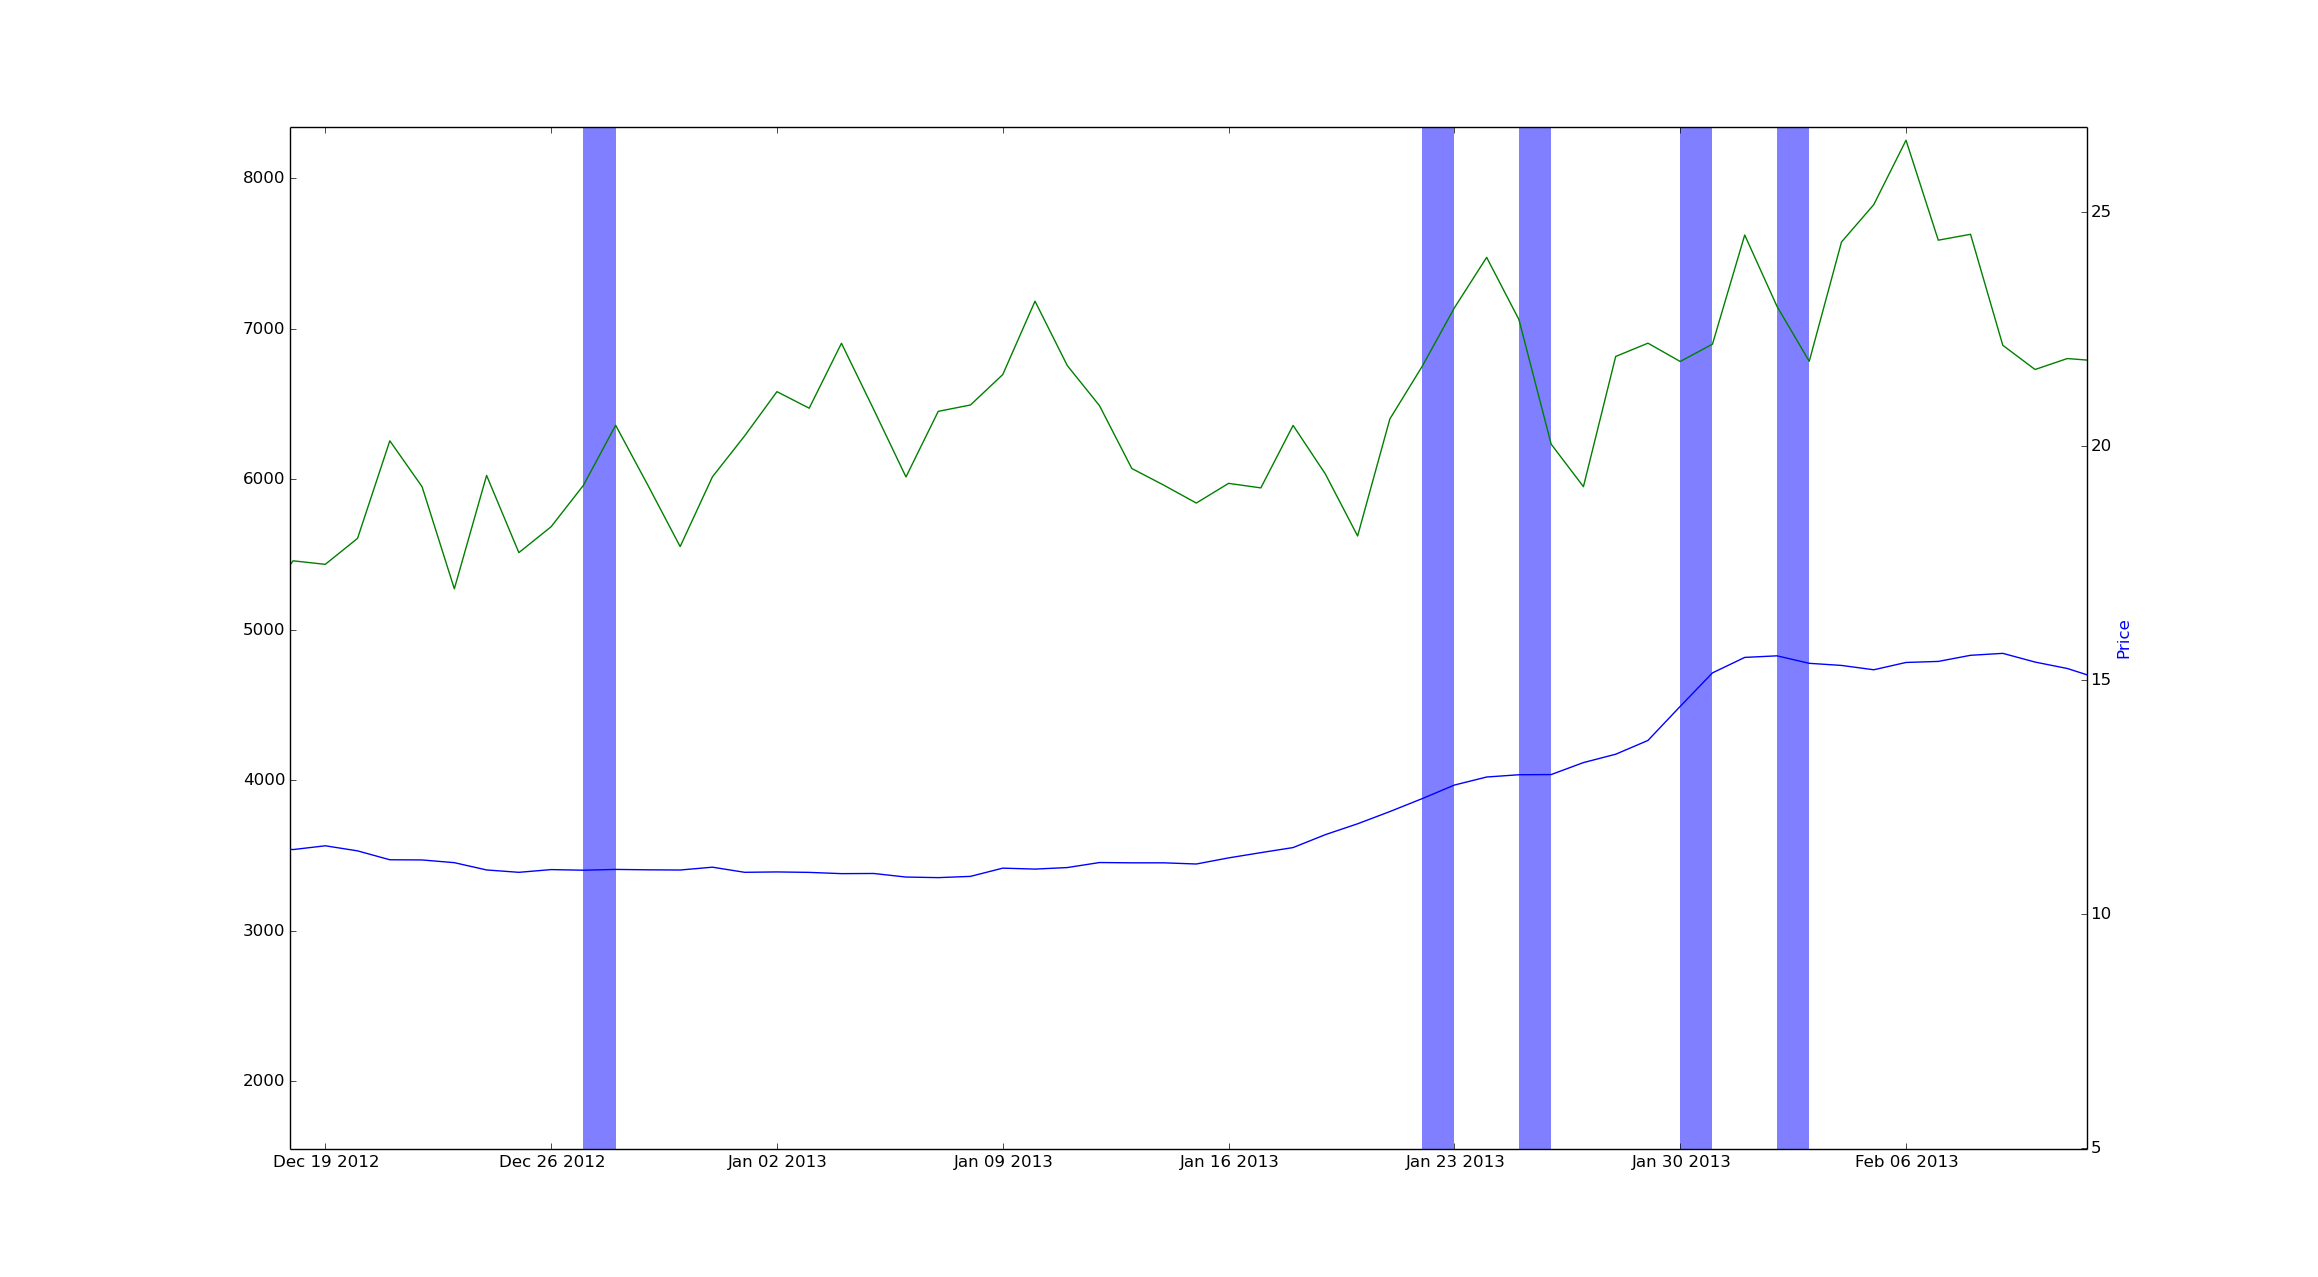
\includegraphics[width=0.8\textwidth]{graphs/12143.png}
		    	\caption{Slope Based Anomaly Detection (Green line - Arrival Data of Onion, Blue Line - Wholesale Price)}
		    	\label{fig:12143}
			\end{figure}
			
			\item There exist some cases where due to low arrival, prices went high and when slowly arrival started entering into market, prices were going down slowly. This period of slow decrement of prices is not reported by this method but since prices were still high, this system could not report dates for news articles corresponding to this tenure. Such cases occurred in \textit{Analysis 2} for Dec 2010 and Jan 2011 (See Figure \ref{fig:12124})and in \textit{Analysis 4} for Nov 2013 (See Figure \ref{fig:12144}). Also, note that these articles were mainly on Pakistan banned exports and article on inflation stating that inflation rate went high and onion prices are playing an important role in this.
			
			\begin{figure}[H]
		    	\centering
  		    	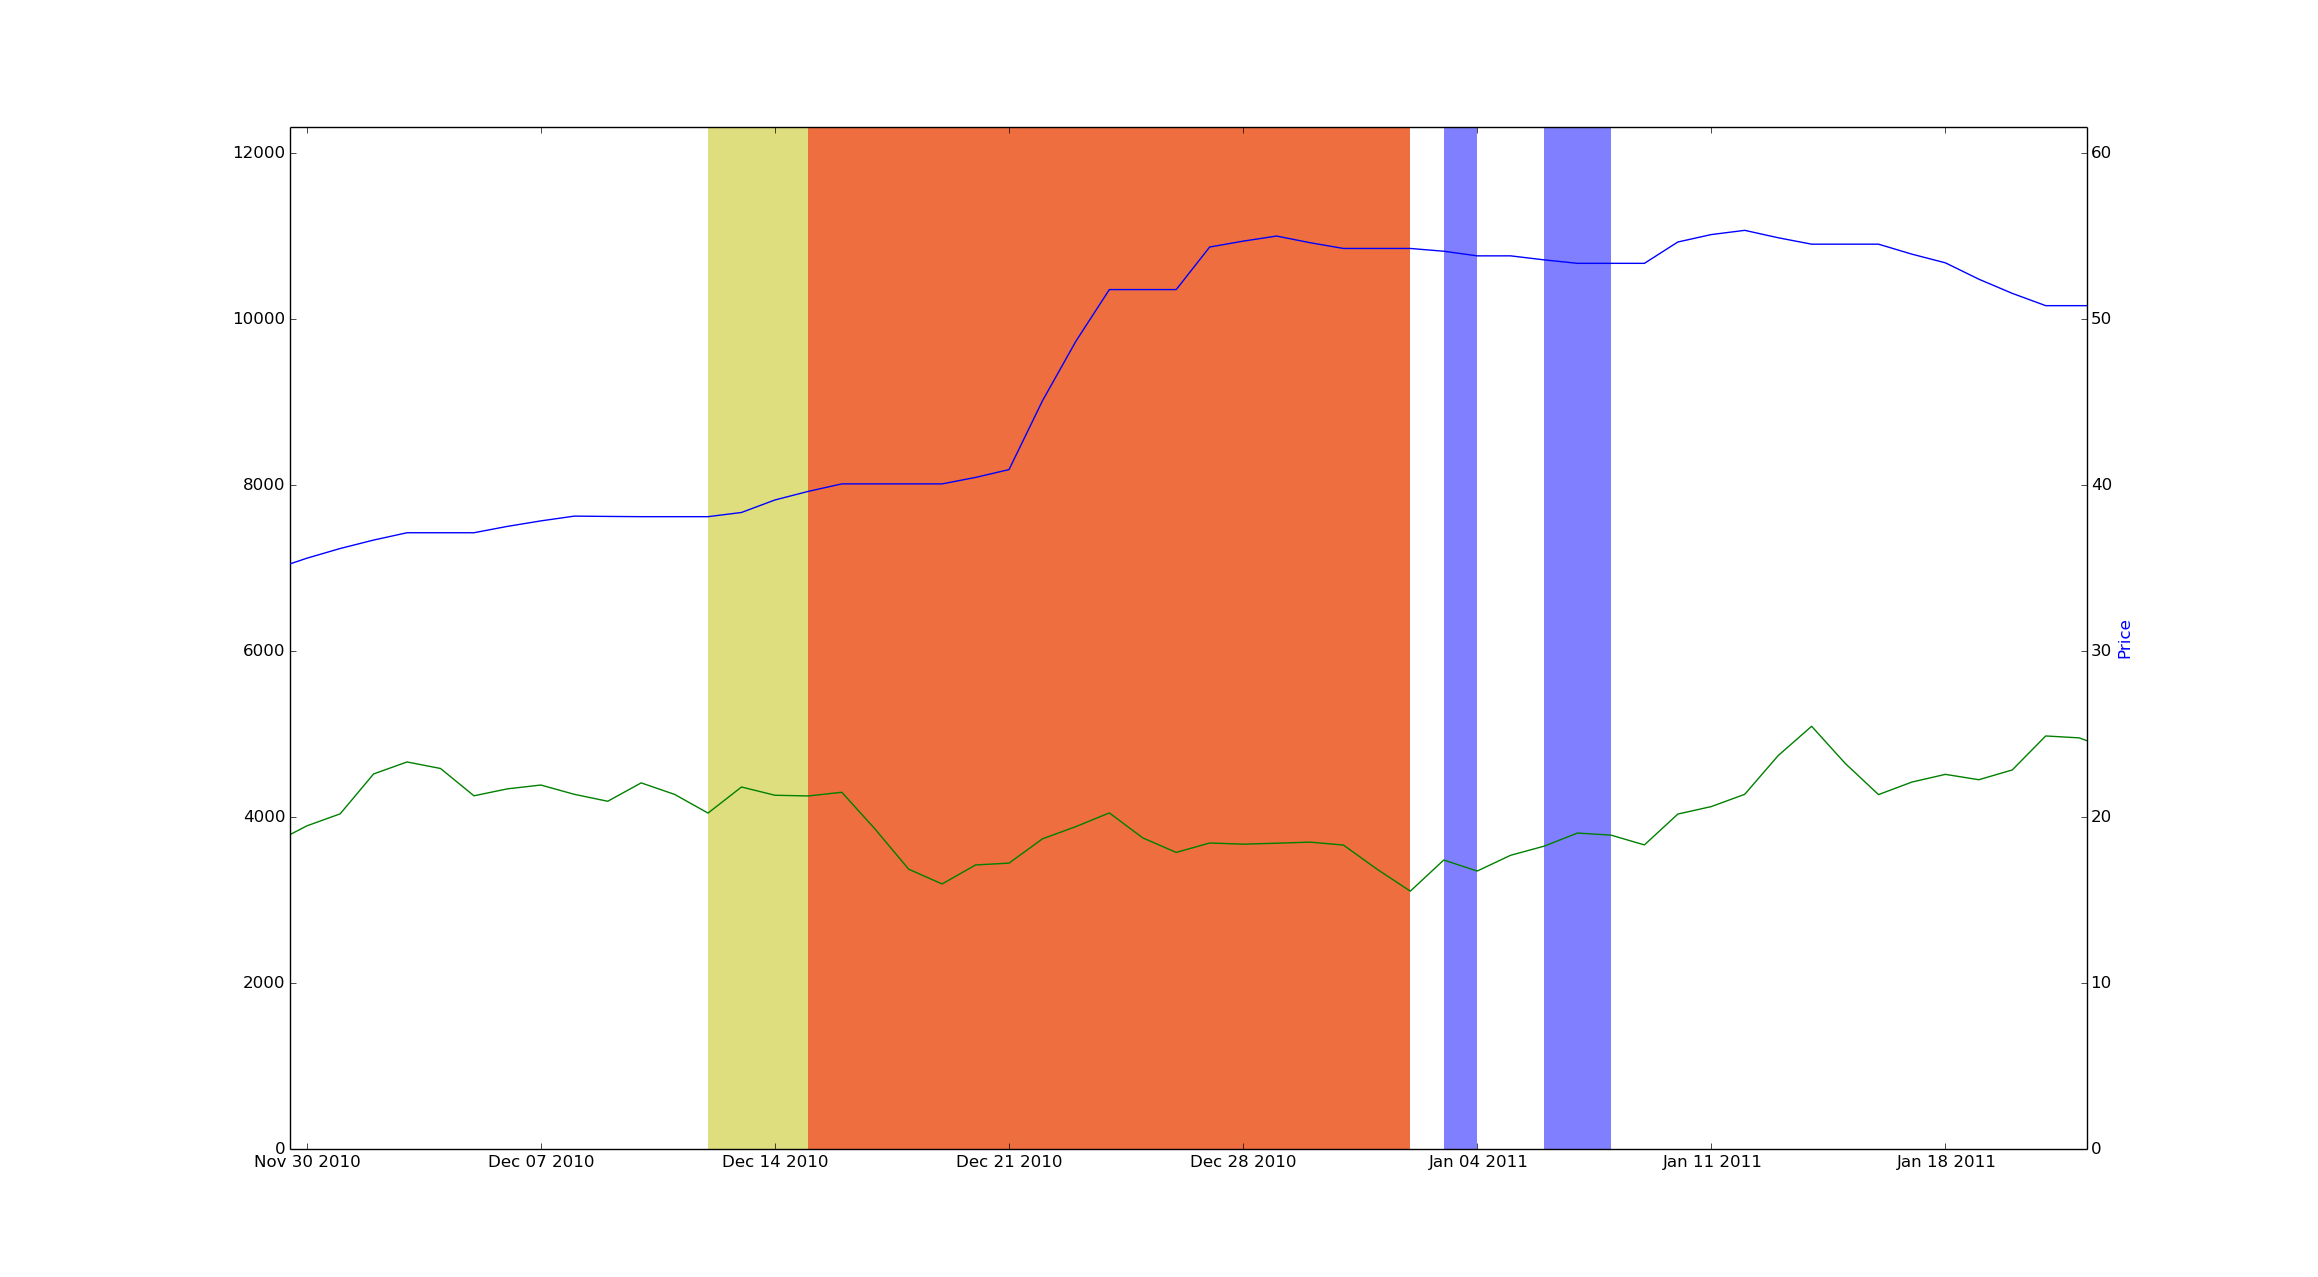
\includegraphics[width=0.8\textwidth]{graphs/12124.png}
		    	\caption{Slope Based Anomaly Detection (Green line - Arrival Data of Onion, Blue Line - Retail Price)}
		    	\label{fig:12124}
			\end{figure}
			
			\begin{figure}[H]
		    	\centering
  		    	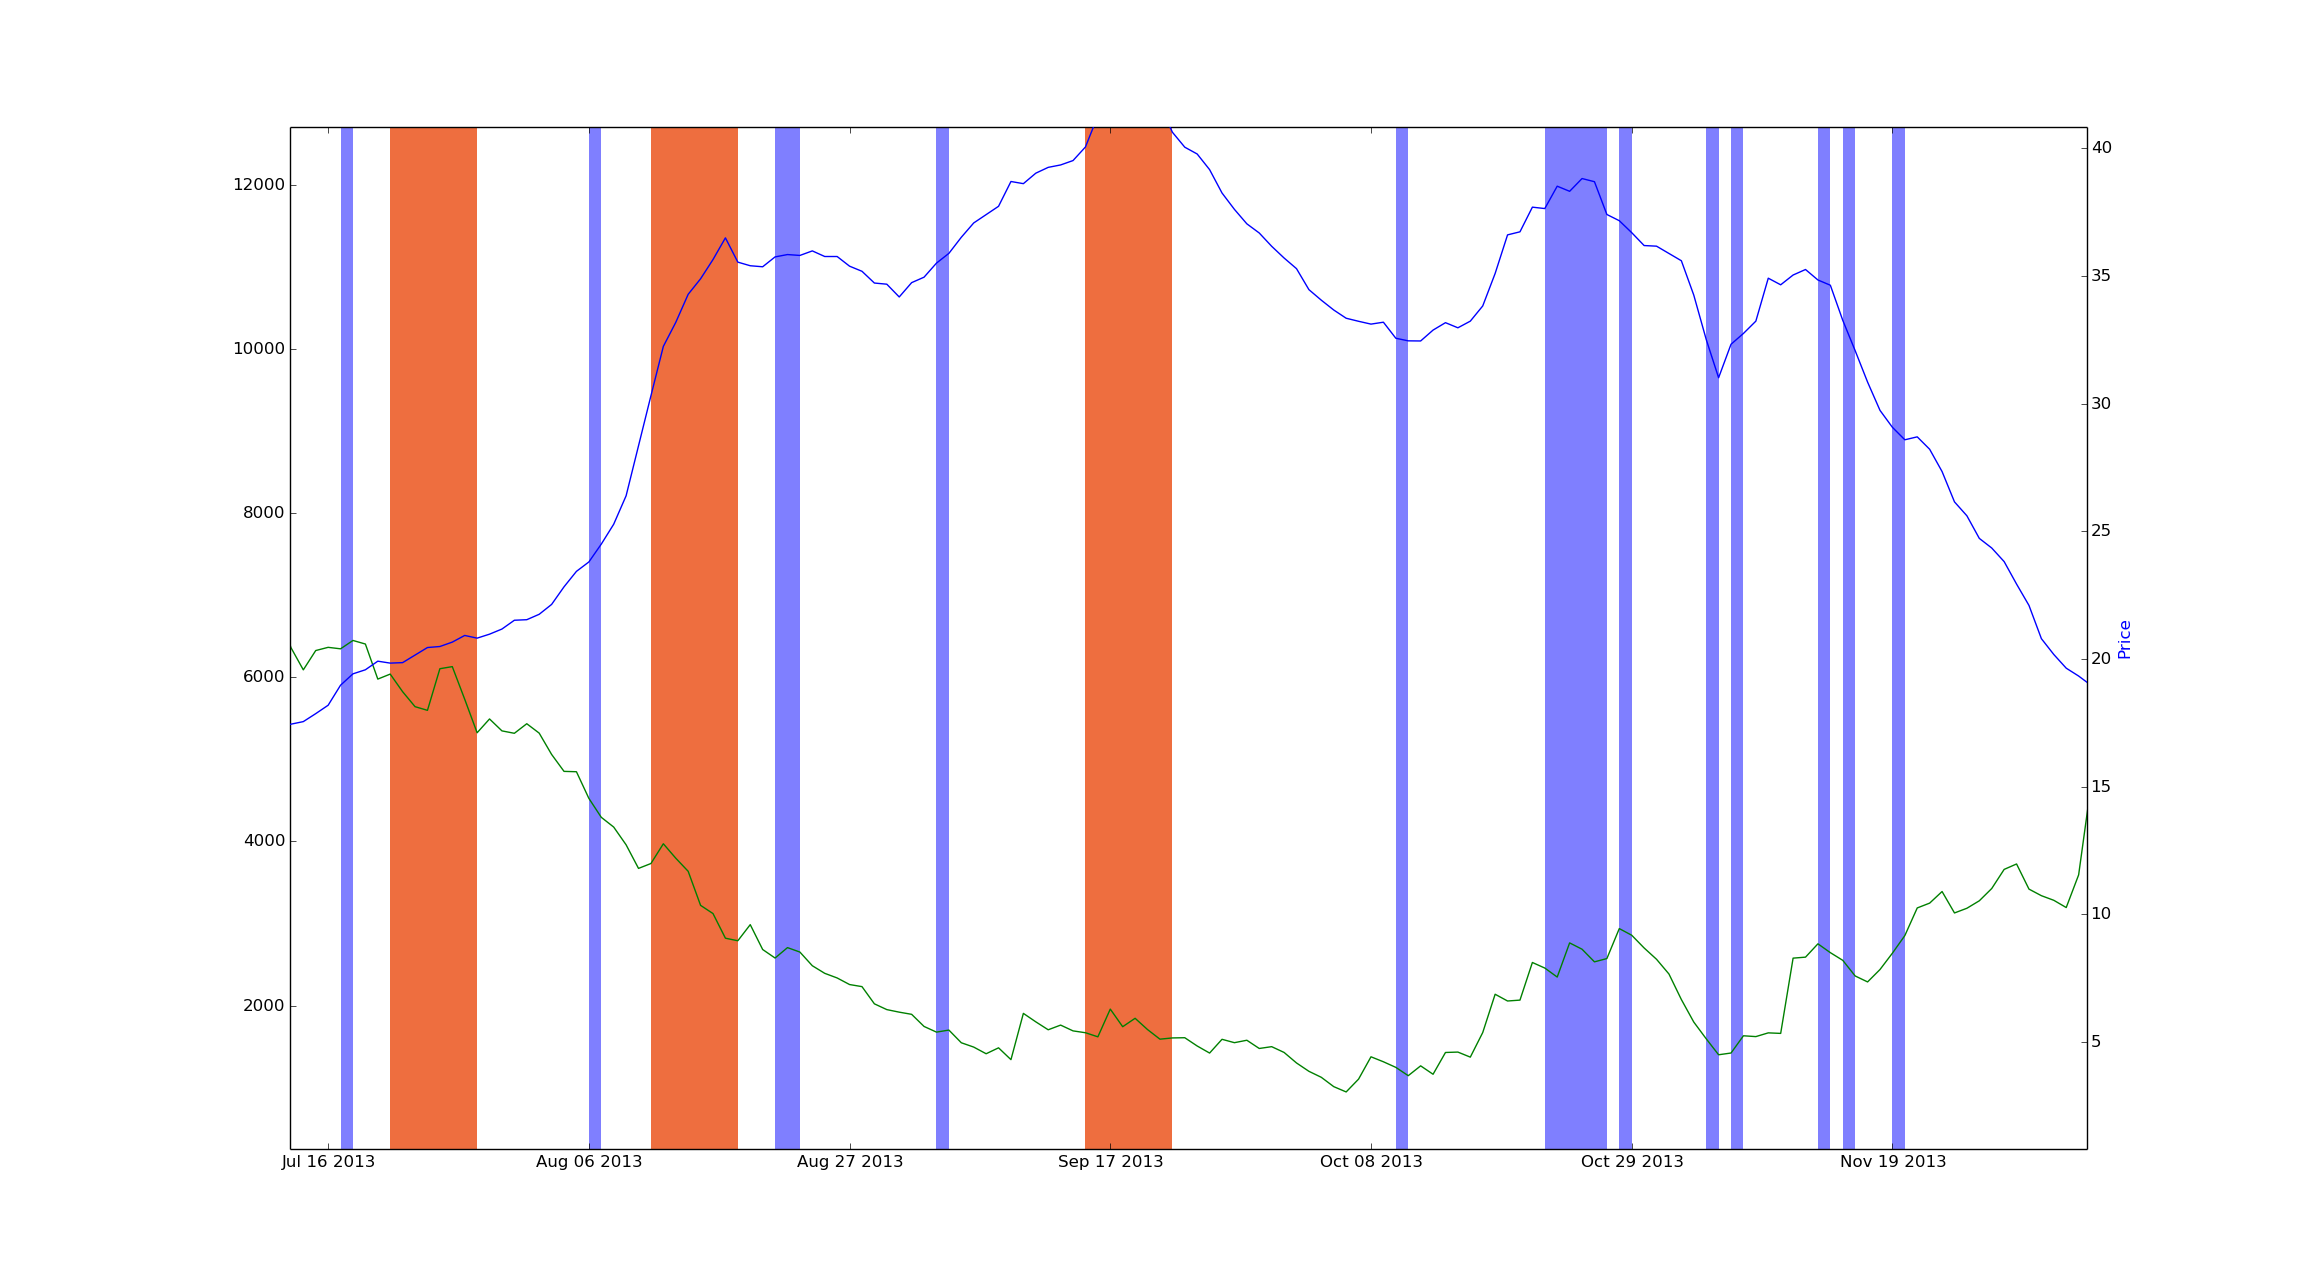
\includegraphics[width=0.8\textwidth]{graphs/12144.png}
		    	\caption{Slope Based Anomaly Detection (Green line - Arrival Data of Onion, Blue Line - Wholesale Price)}
		    	\label{fig:12144}
			\end{figure}
			
			\item In some of the cases where arrival fell drastically and due to that retail price went high drastically. Since retail prices went high too much, it got reported in news articles but this was expected as arrival was less. But here both the changes were high, so ultimately slope value was not so high and was not reported by system. Such cases in \textit{Analysis 2} exist for Aug Sept 2013  (See Figure \ref{fig:12125}).
			
			\begin{figure}[H]
		    	\centering
  		    	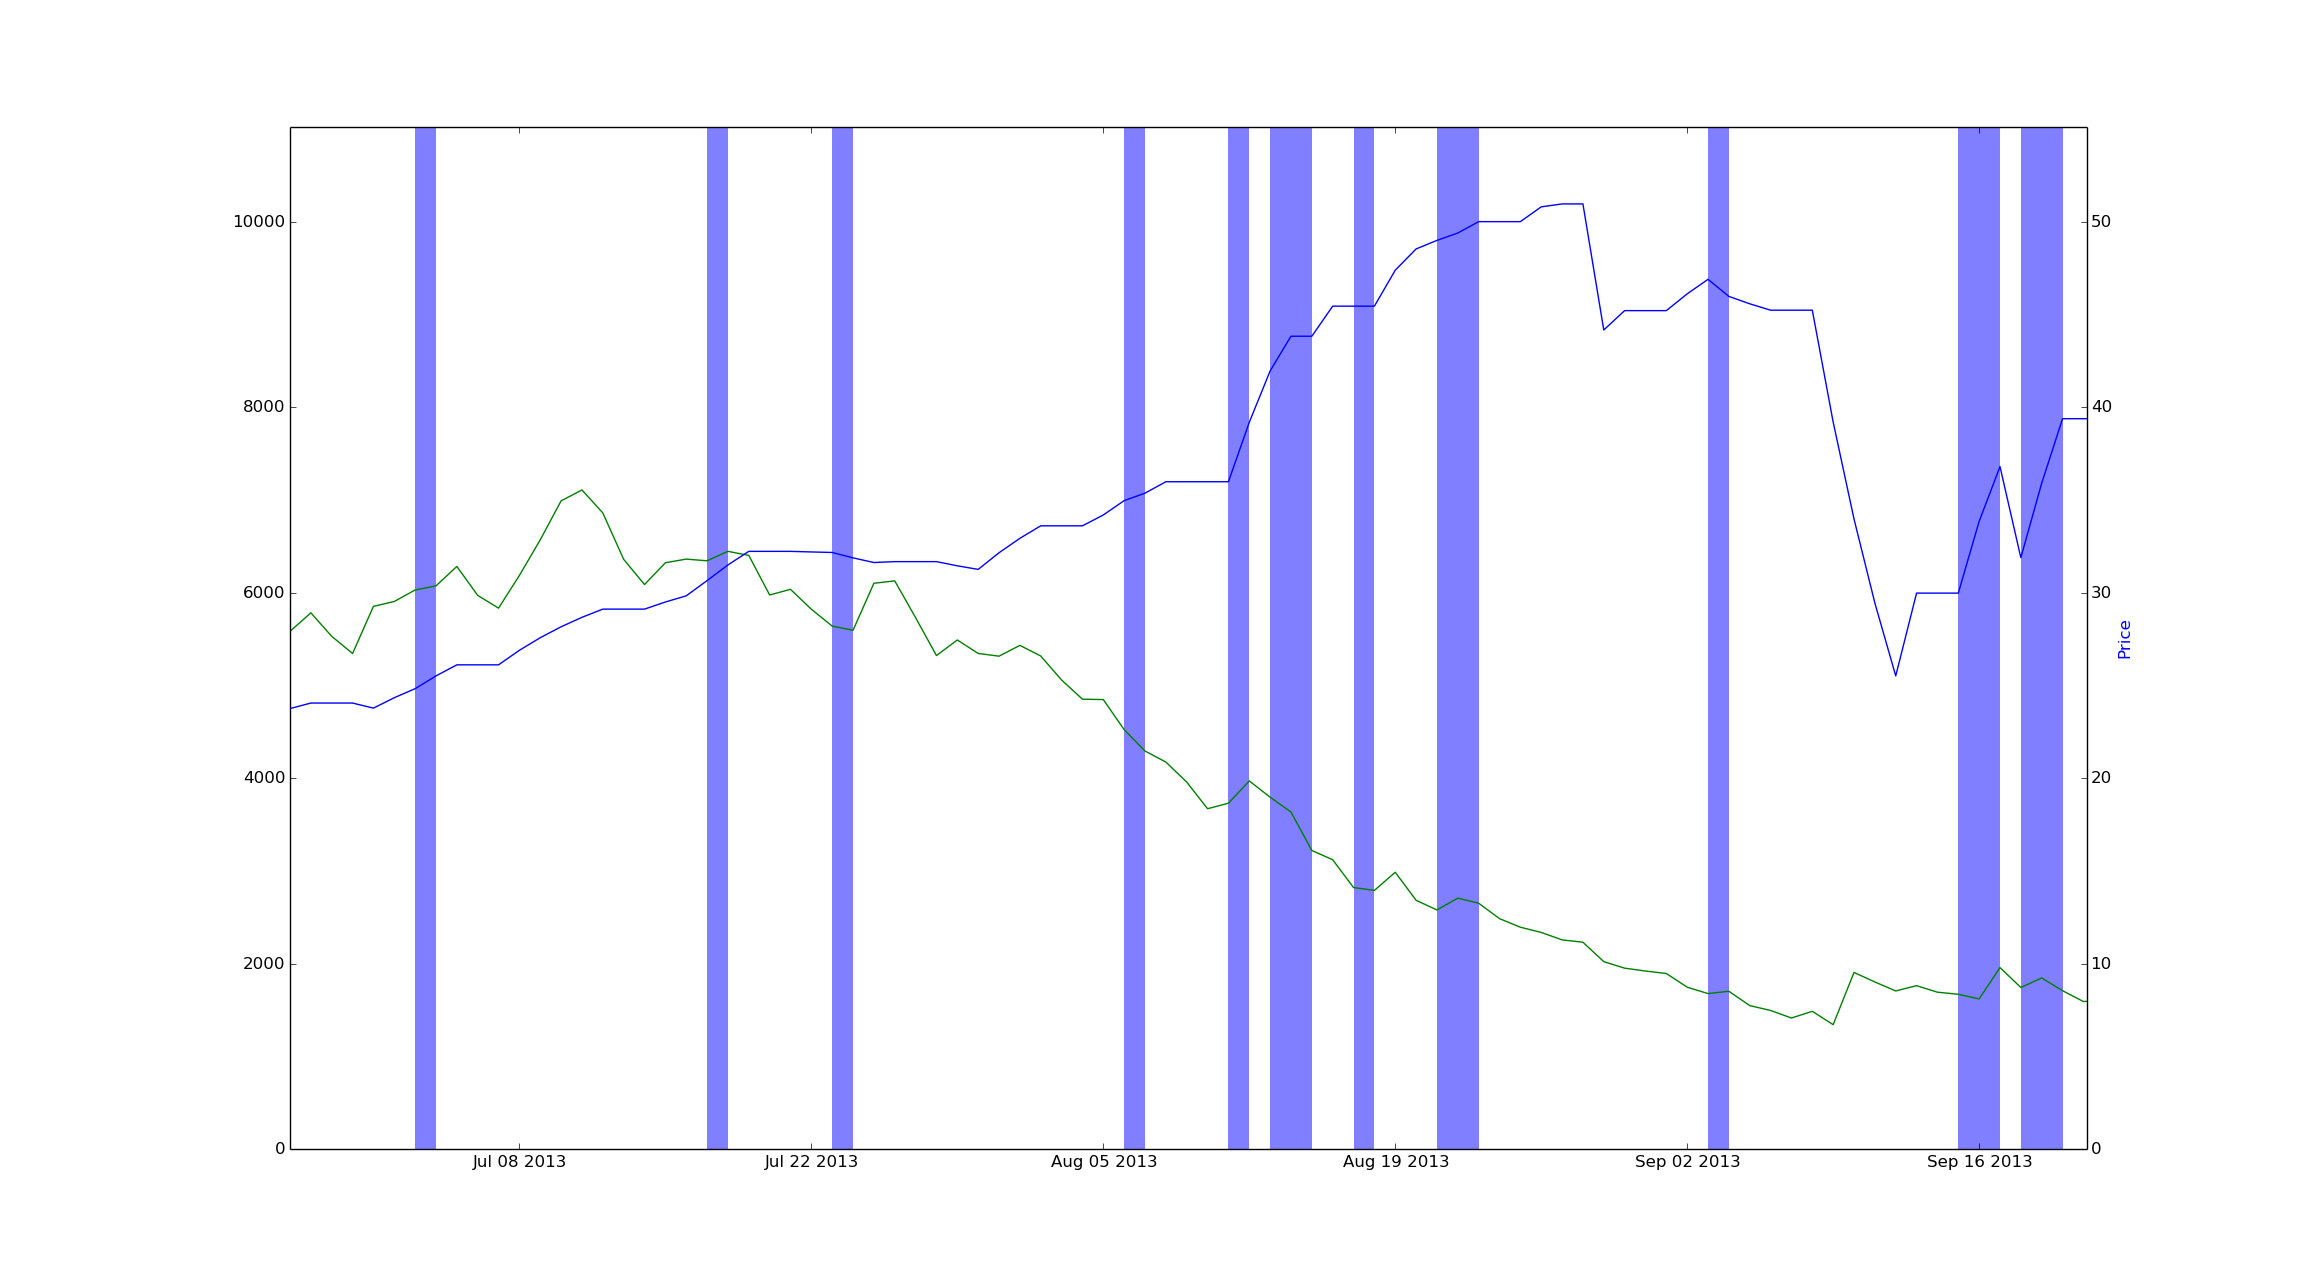
\includegraphics[width=0.8\textwidth]{graphs/12125.png}
		    	\caption{Slope Based Anomaly Detection (Green line - Arrival Data of Onion, Blue Line - Retail Price)}
		    	\label{fig:12125}
			\end{figure}
			
			\item Another limitation of this method is when retail price remained constant and there was change in arrival. As retail price was constant, slope value became zero and method did not report them and due to that few news articles could not be matched by dates reported by this method for example in \textit{Analysis 2}, this thing occurred for June July 2015  (See Figure \ref{fig:12126}).
			
			\begin{figure}[H]
		    	\centering
  		    	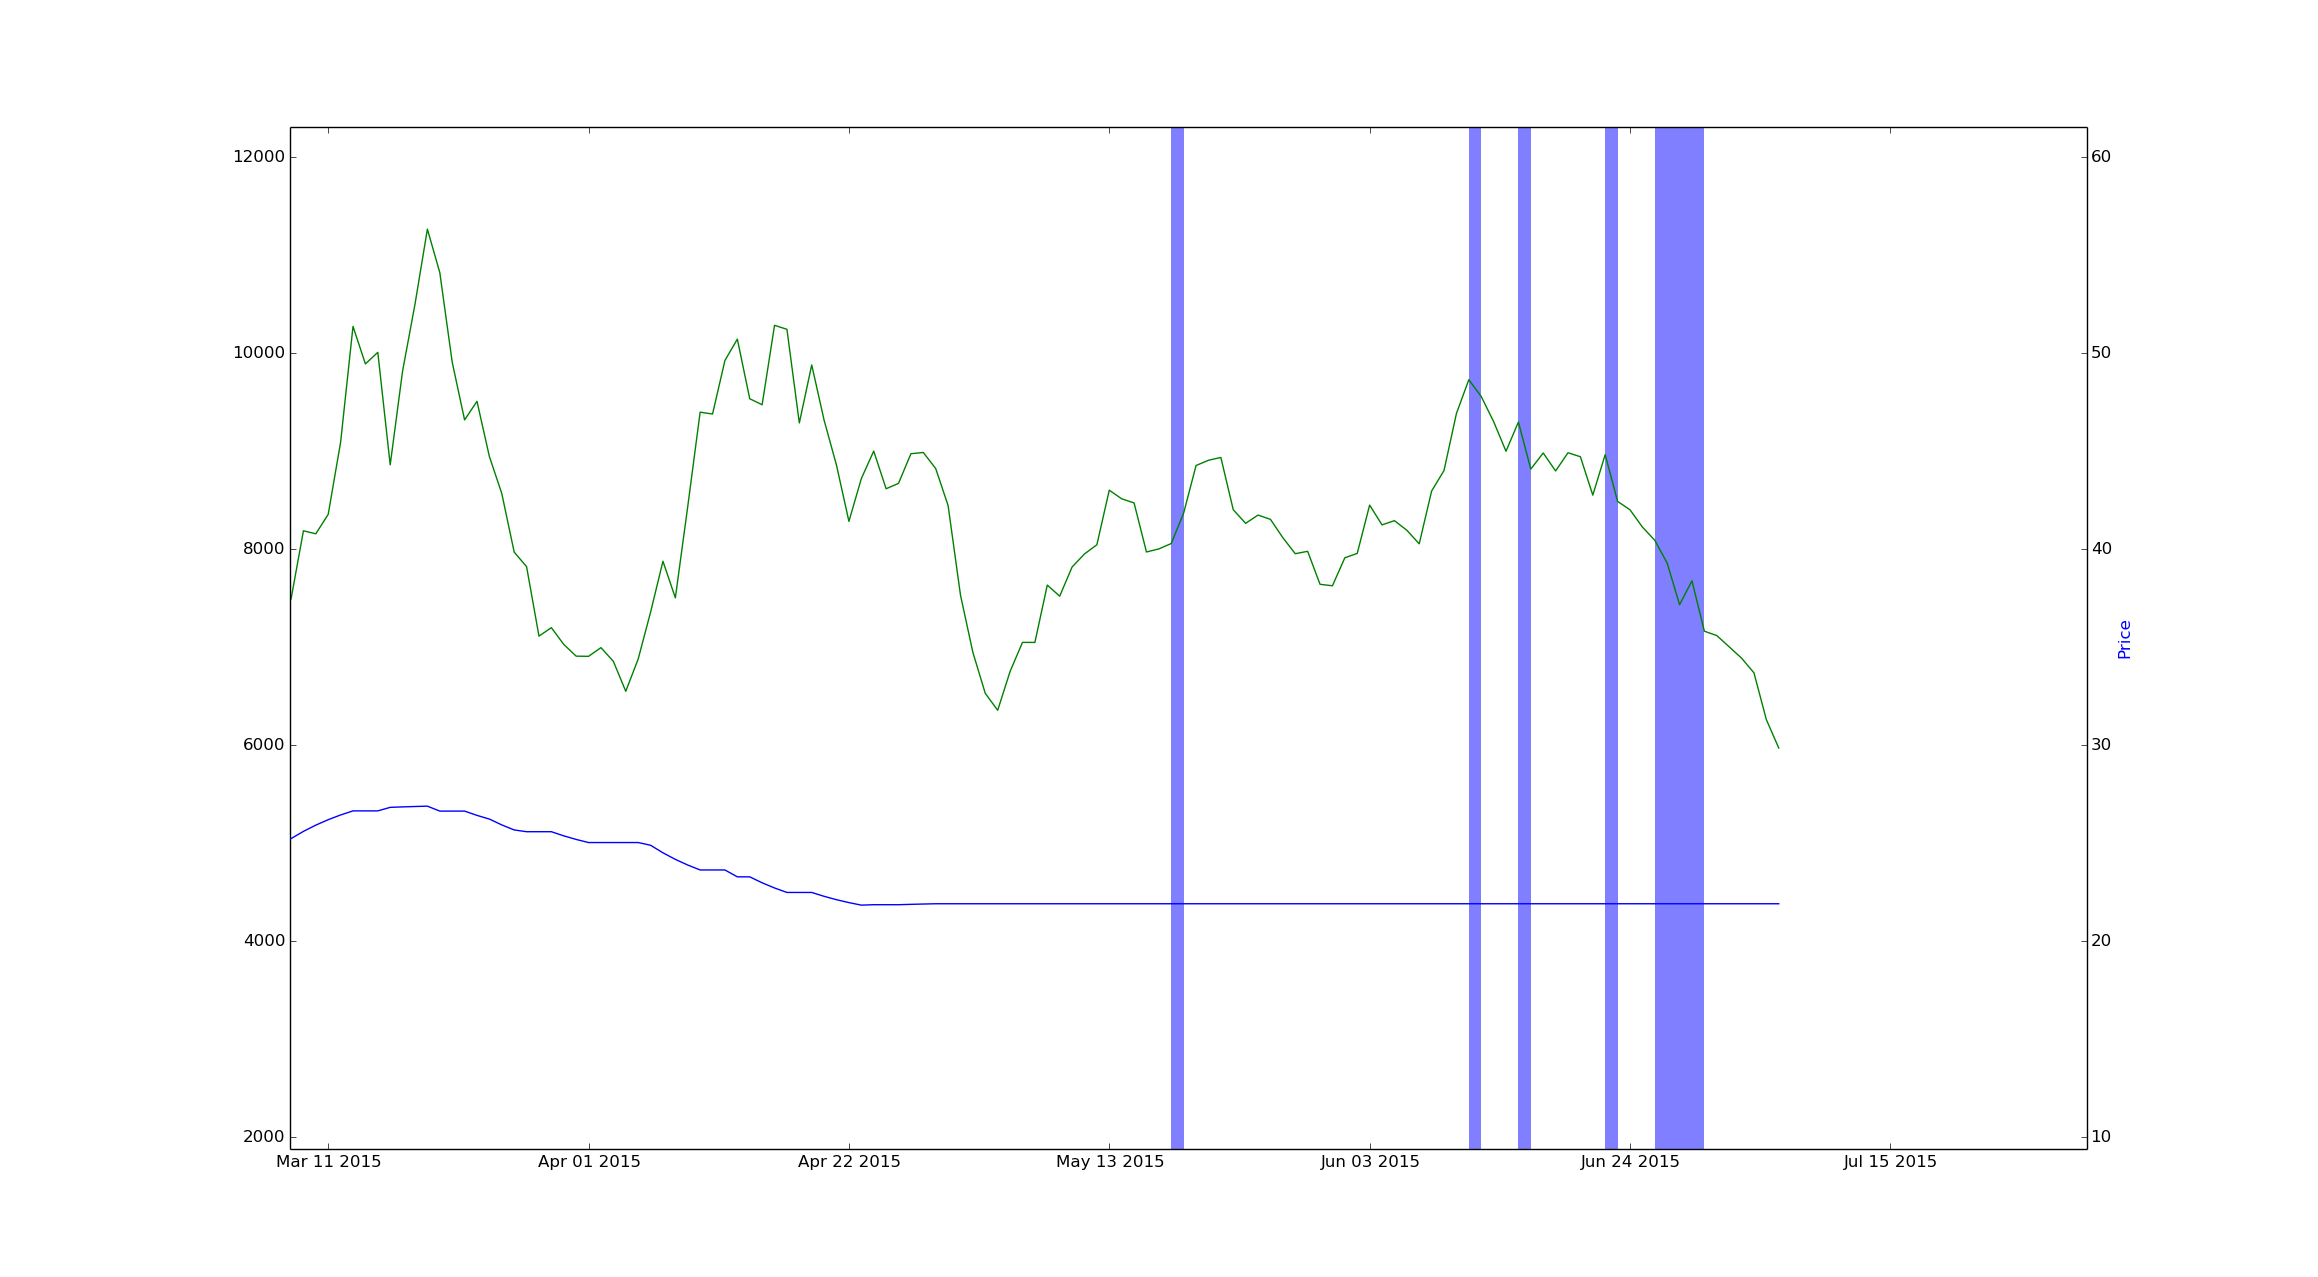
\includegraphics[width=0.8\textwidth]{graphs/12126.png}
		    	\caption{Slope Based Anomaly Detection (Green line - Arrival Data of Onion, Blue Line - Retail Price)}
		    	\label{fig:12126}
			\end{figure}
			
		\end{itemize}


	Also, note one thing that this method reports anomaly as whole window of few days (here 7 days). So because of that too, method tends to report more anomaly dates.


\subsection{Linear Regression}

		The main functionality of this method is to find what should be ideal value of the dependent variable given value of independent variable. This method first finds out linear relationship between 2 variables, whose time series is given as input and one of them is dependent on another. After finding out this equation, we see for a given value of independent variable what should be ideal value of dependent variable and note down the relative difference. If this difference is large, then it is reported as anomaly.\\
		\\
		We have four types of analysis which are as follows:
		\begin{enumerate}
			\item \textbf{Retail Price vs Average of Retail Price}: Here, we first take average of retail price at all centres as independent variable and retail price as dependent variable.			
			\item \textbf{Retail Price vs Arrival of Onion}: Here, we take retail price as dependent variable and arrival of onion as independent variable.
			\item \textbf{Retail Price vs Wholesale Price}: Here, we take retail price as dependent variable and Wholesale Price as independent variable.
			\item \textbf{Wholesale Price vs Arrival of Onion}: Here, we take Wholesale price as dependent variable and arrival of onion as independent variable.
		\end{enumerate}
		
		So, in each of the case, we try to find relative difference between ideal value and its real value, and if it is huge (crosses threshold) then it is reported as anomaly. Now, note that in analysis 1 and 3 stated above, both the time series are directly proportional to each other and in the analysis 2 and 4 both the time series are inversely proportional to each other. So, limitations faced by this method for analysis 1 and 3 will be similar and for analysis 2 and 4 will be similar. While describing this method, each analysis will be referenced by its corresponding number.\\
		\\
		First we will start with analysis 1 and 3. Following are the few observations we made:
		
		\begin{itemize}
			\item This method will report any tenure as anomaly when there is large gap i.e. more than expected between retail price of a center and average retail price (for \textit{Analysis 1}) or wholesale price (for \textit{Analysis 3}).
			
			
			
			Following tenures are some cases reported by this method:
			\begin{itemize}
				\item \textit{Analysis 1}: Dec 2010, Near to Jan 2011, May June July 2011, Jan May June 2012, June 2013 (See Figure \ref{fig:12211})
				\item \textit{Analysis 3}: Feb Mar 2011, Jan 2012, June 2012, Jan Feb 2014, Apr 2015 (See Figure \ref{fig:12231})
			\end{itemize}
			\begin{figure}[H]
		    	\centering
  		    	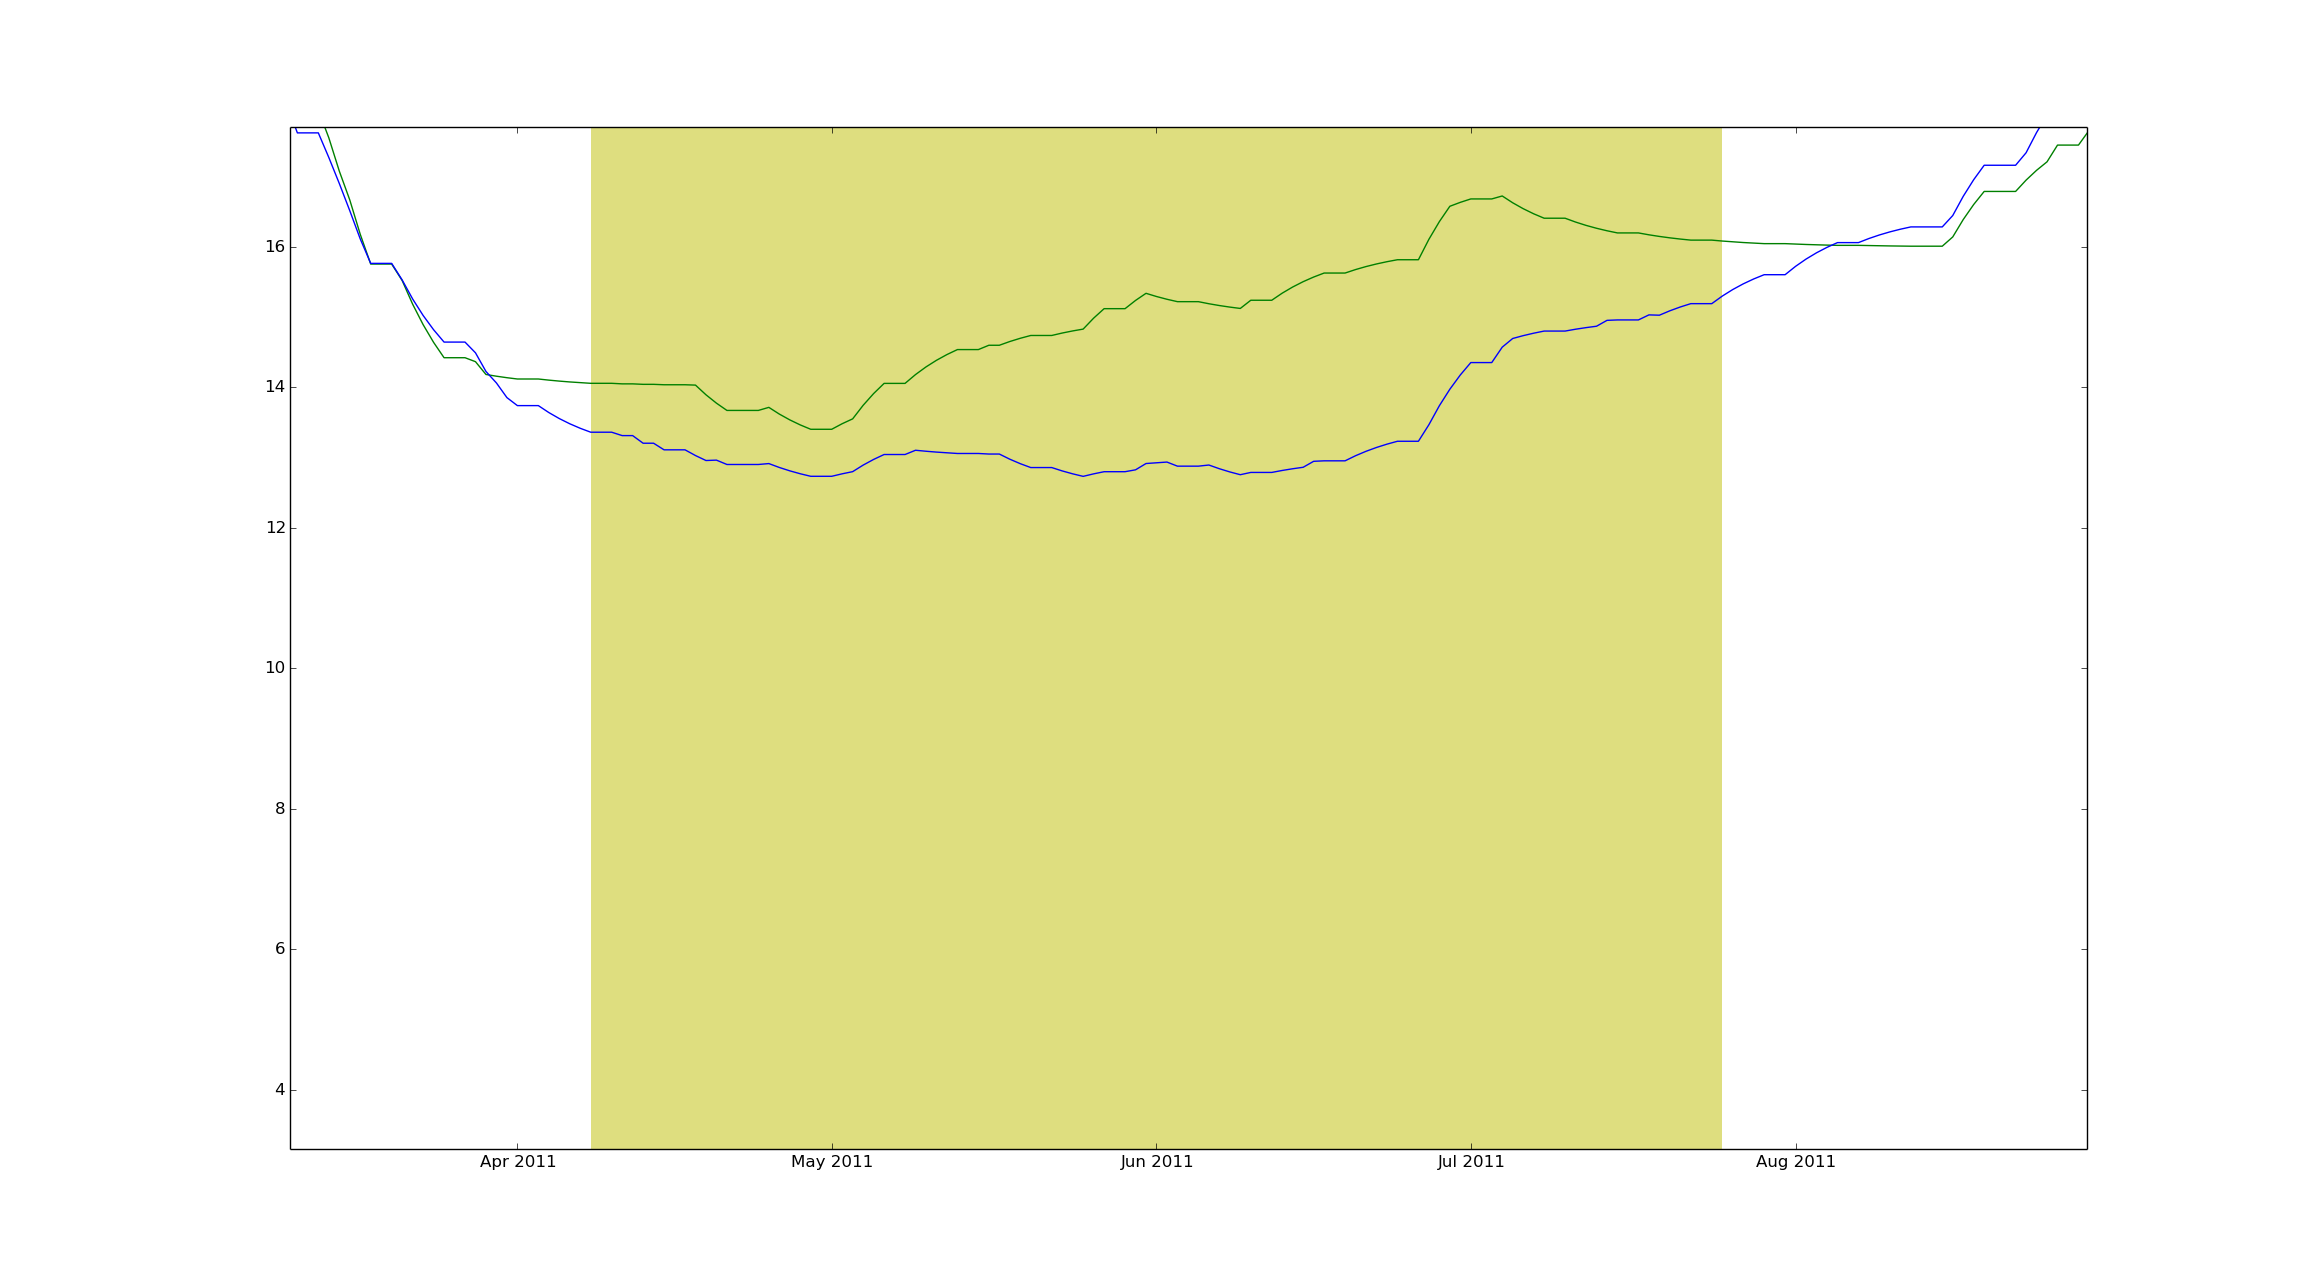
\includegraphics[width=0.8\textwidth]{graphs/12211.png}
		    	\caption{Linear Regression (Green line - Centre Retail Price, Blue Line - Average Retail Price)}
		    	\label{fig:12211}
			\end{figure}
			
			\begin{figure}[H]
		    	\centering
  		    	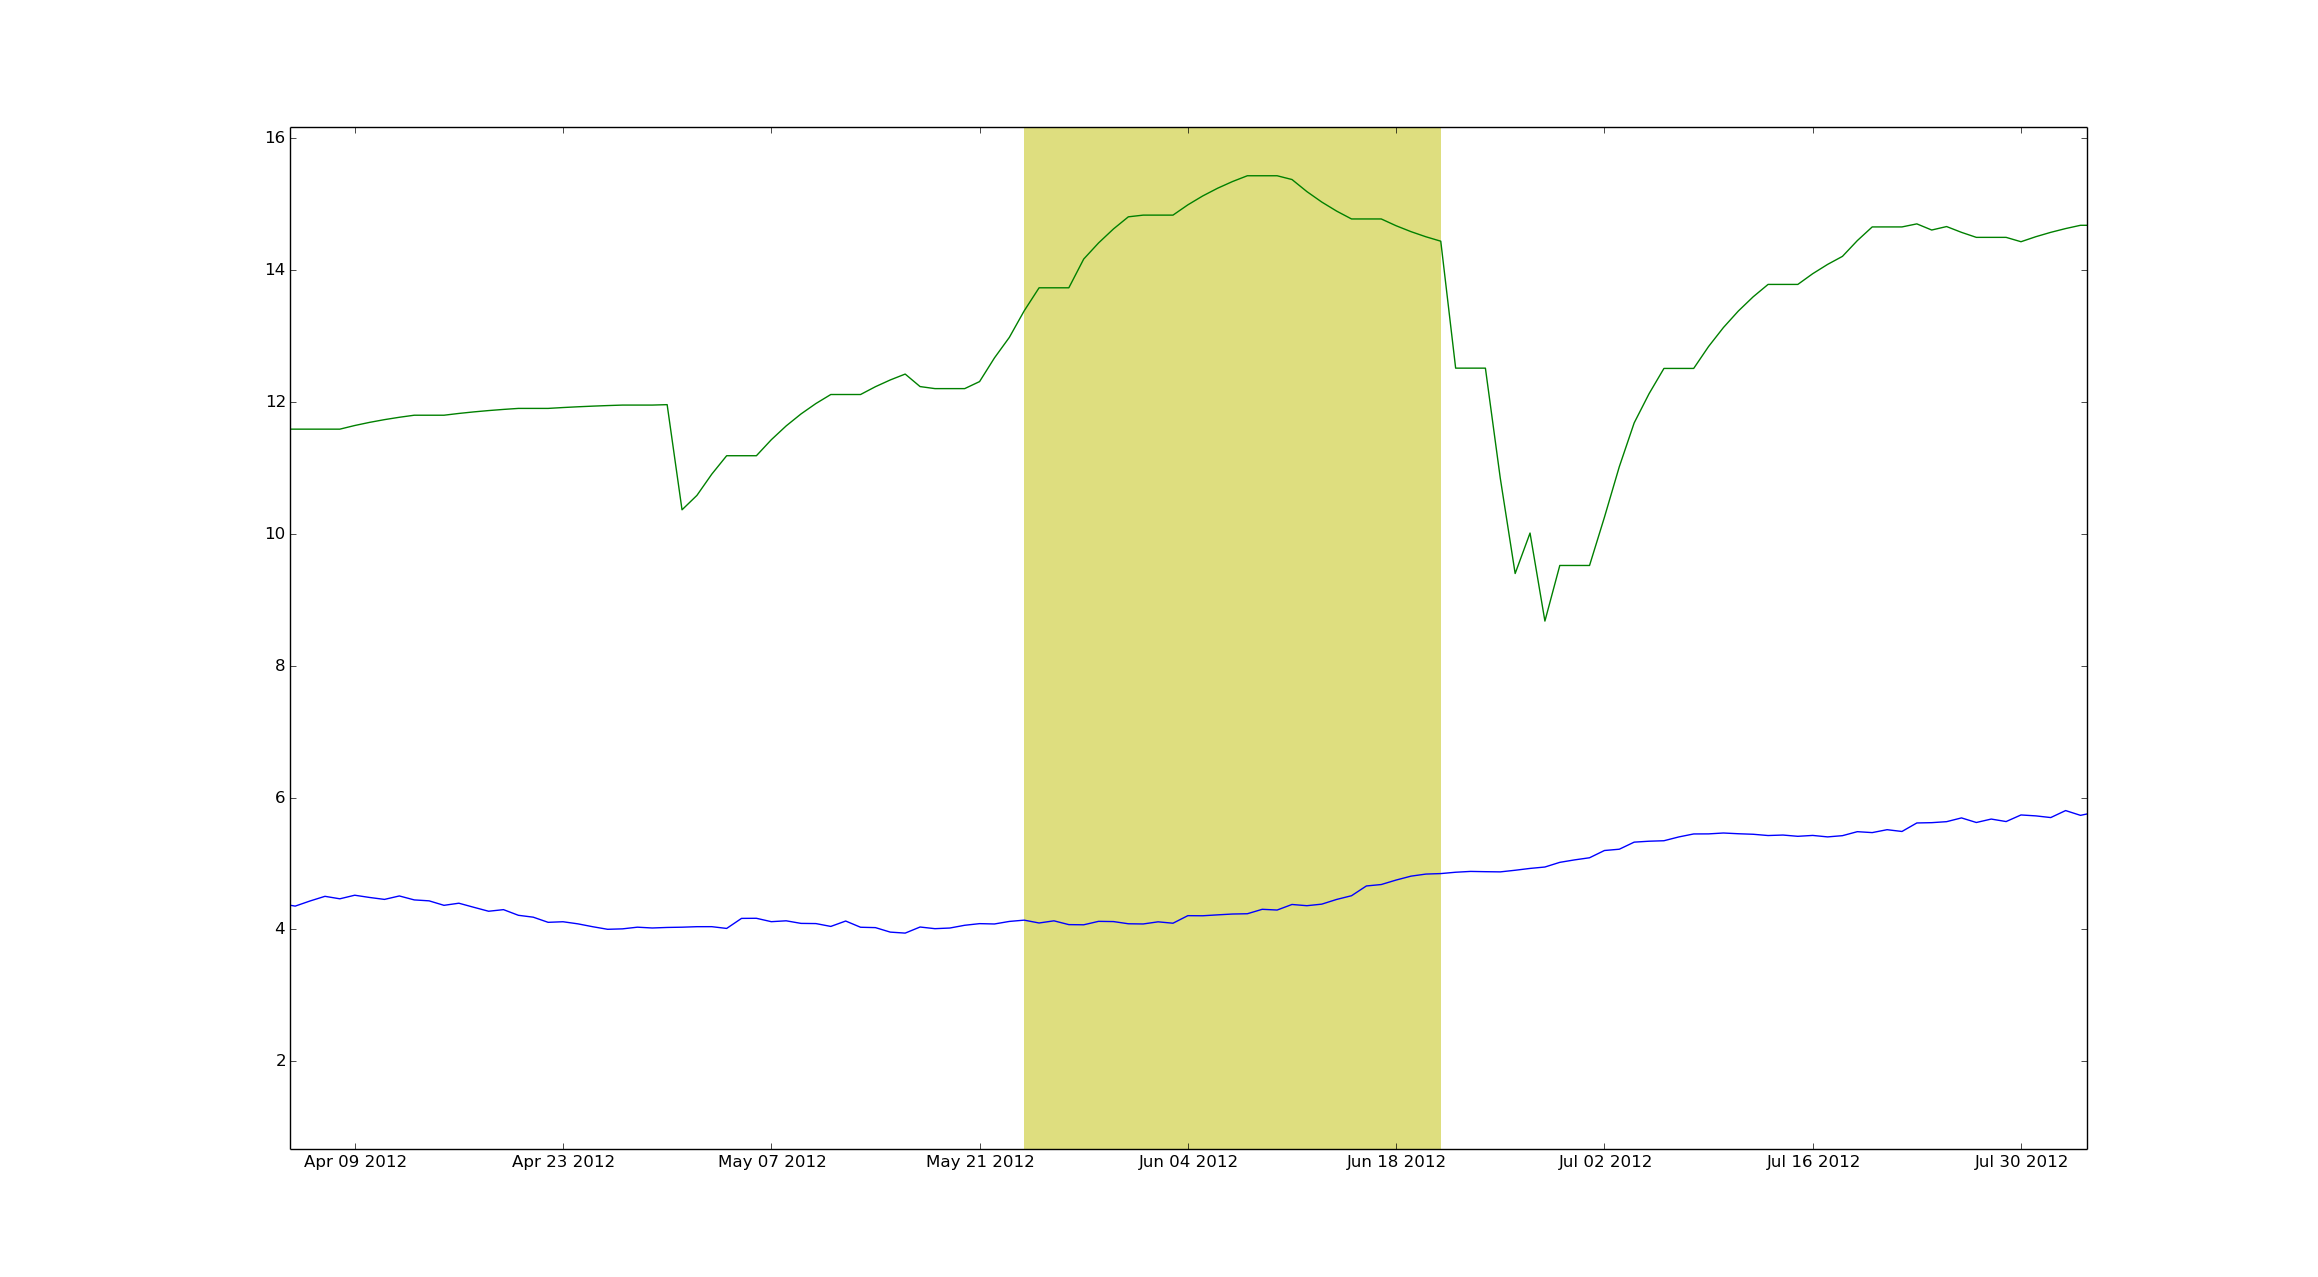
\includegraphics[width=0.8\textwidth]{graphs/12231.png}
		    	\caption{Linear Regression (Green line - Retail Price, Blue Line - Wholesale Price)}
		    	\label{fig:12231}
			\end{figure}
			
			\item One limitation of this method is that, if both the series have high values for some time period and difference between them is not so huge then that will not be reported as anomaly.	\\
			\\
			Following tenures are some cases reported by this method:
			\begin{itemize}
				\item \textit{Analysis 1}: Jan 2011, Jan Feb Aug Sept Oct Nov 2013, July 2014, June July 2015 (See Figure \ref{fig:12212})
				\item \textit{Analysis 3}: Feb 2013, Aug Sept Oct Nov 2013, June July 2015 (See Figure \ref{fig:12232})
			\end{itemize}
			\begin{figure}[H]
		    	\centering
  		    	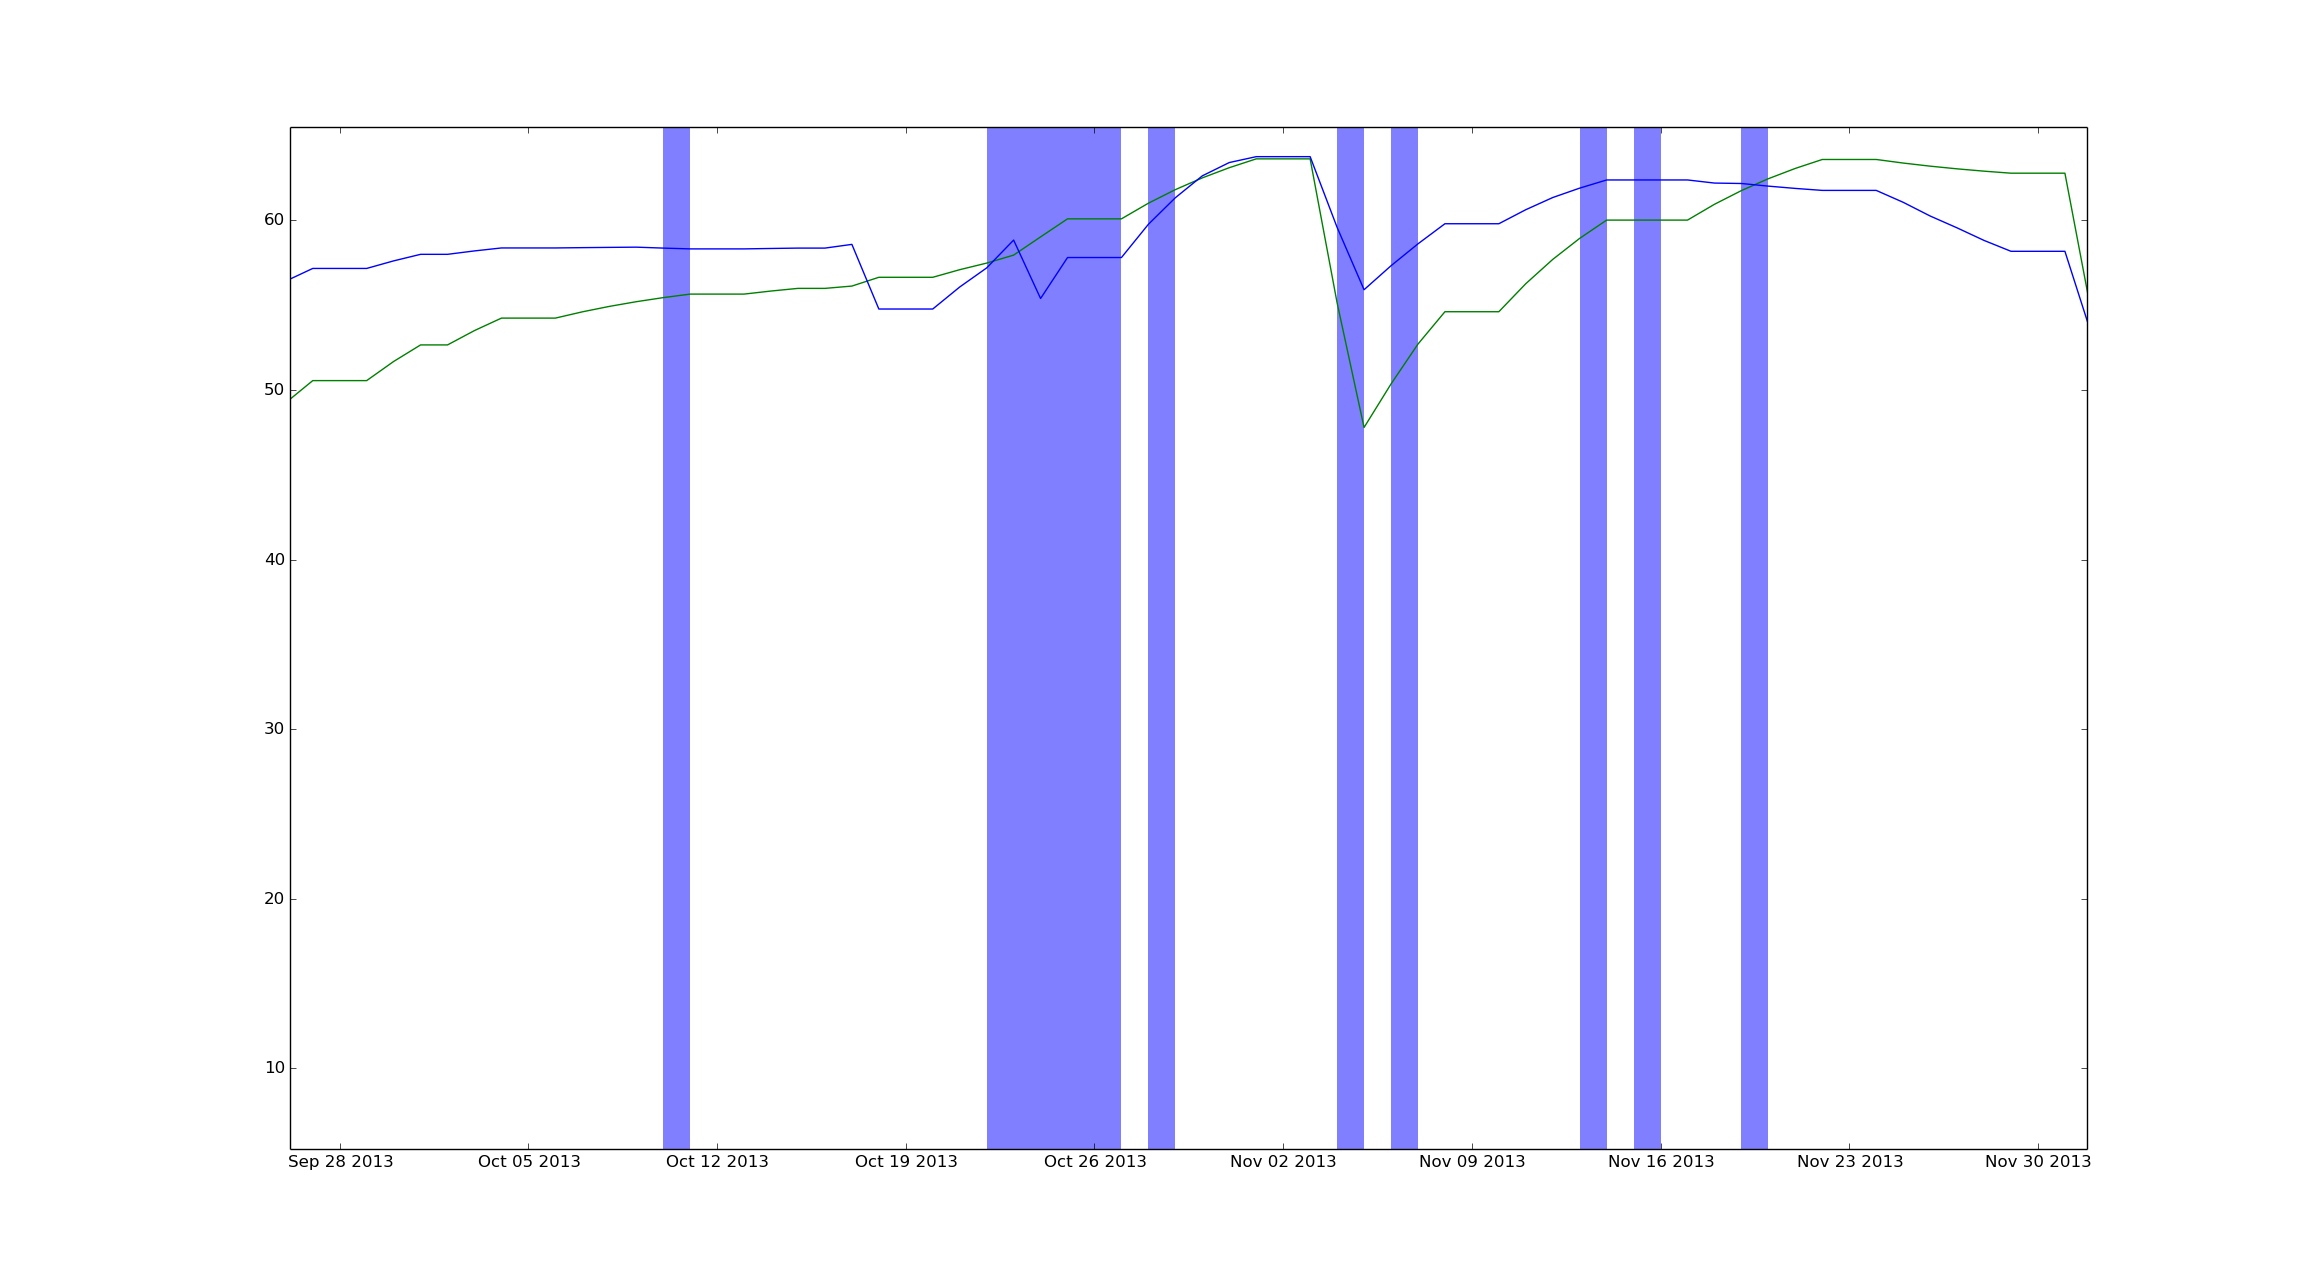
\includegraphics[width=0.8\textwidth]{graphs/12212.png}
		    	\caption{Linear Regression (Green line - Centre Retail Price, Blue Line - Average Retail Price)}
		    	\label{fig:12212}
			\end{figure}
			
			\begin{figure}[H]
		    	\centering
  		    	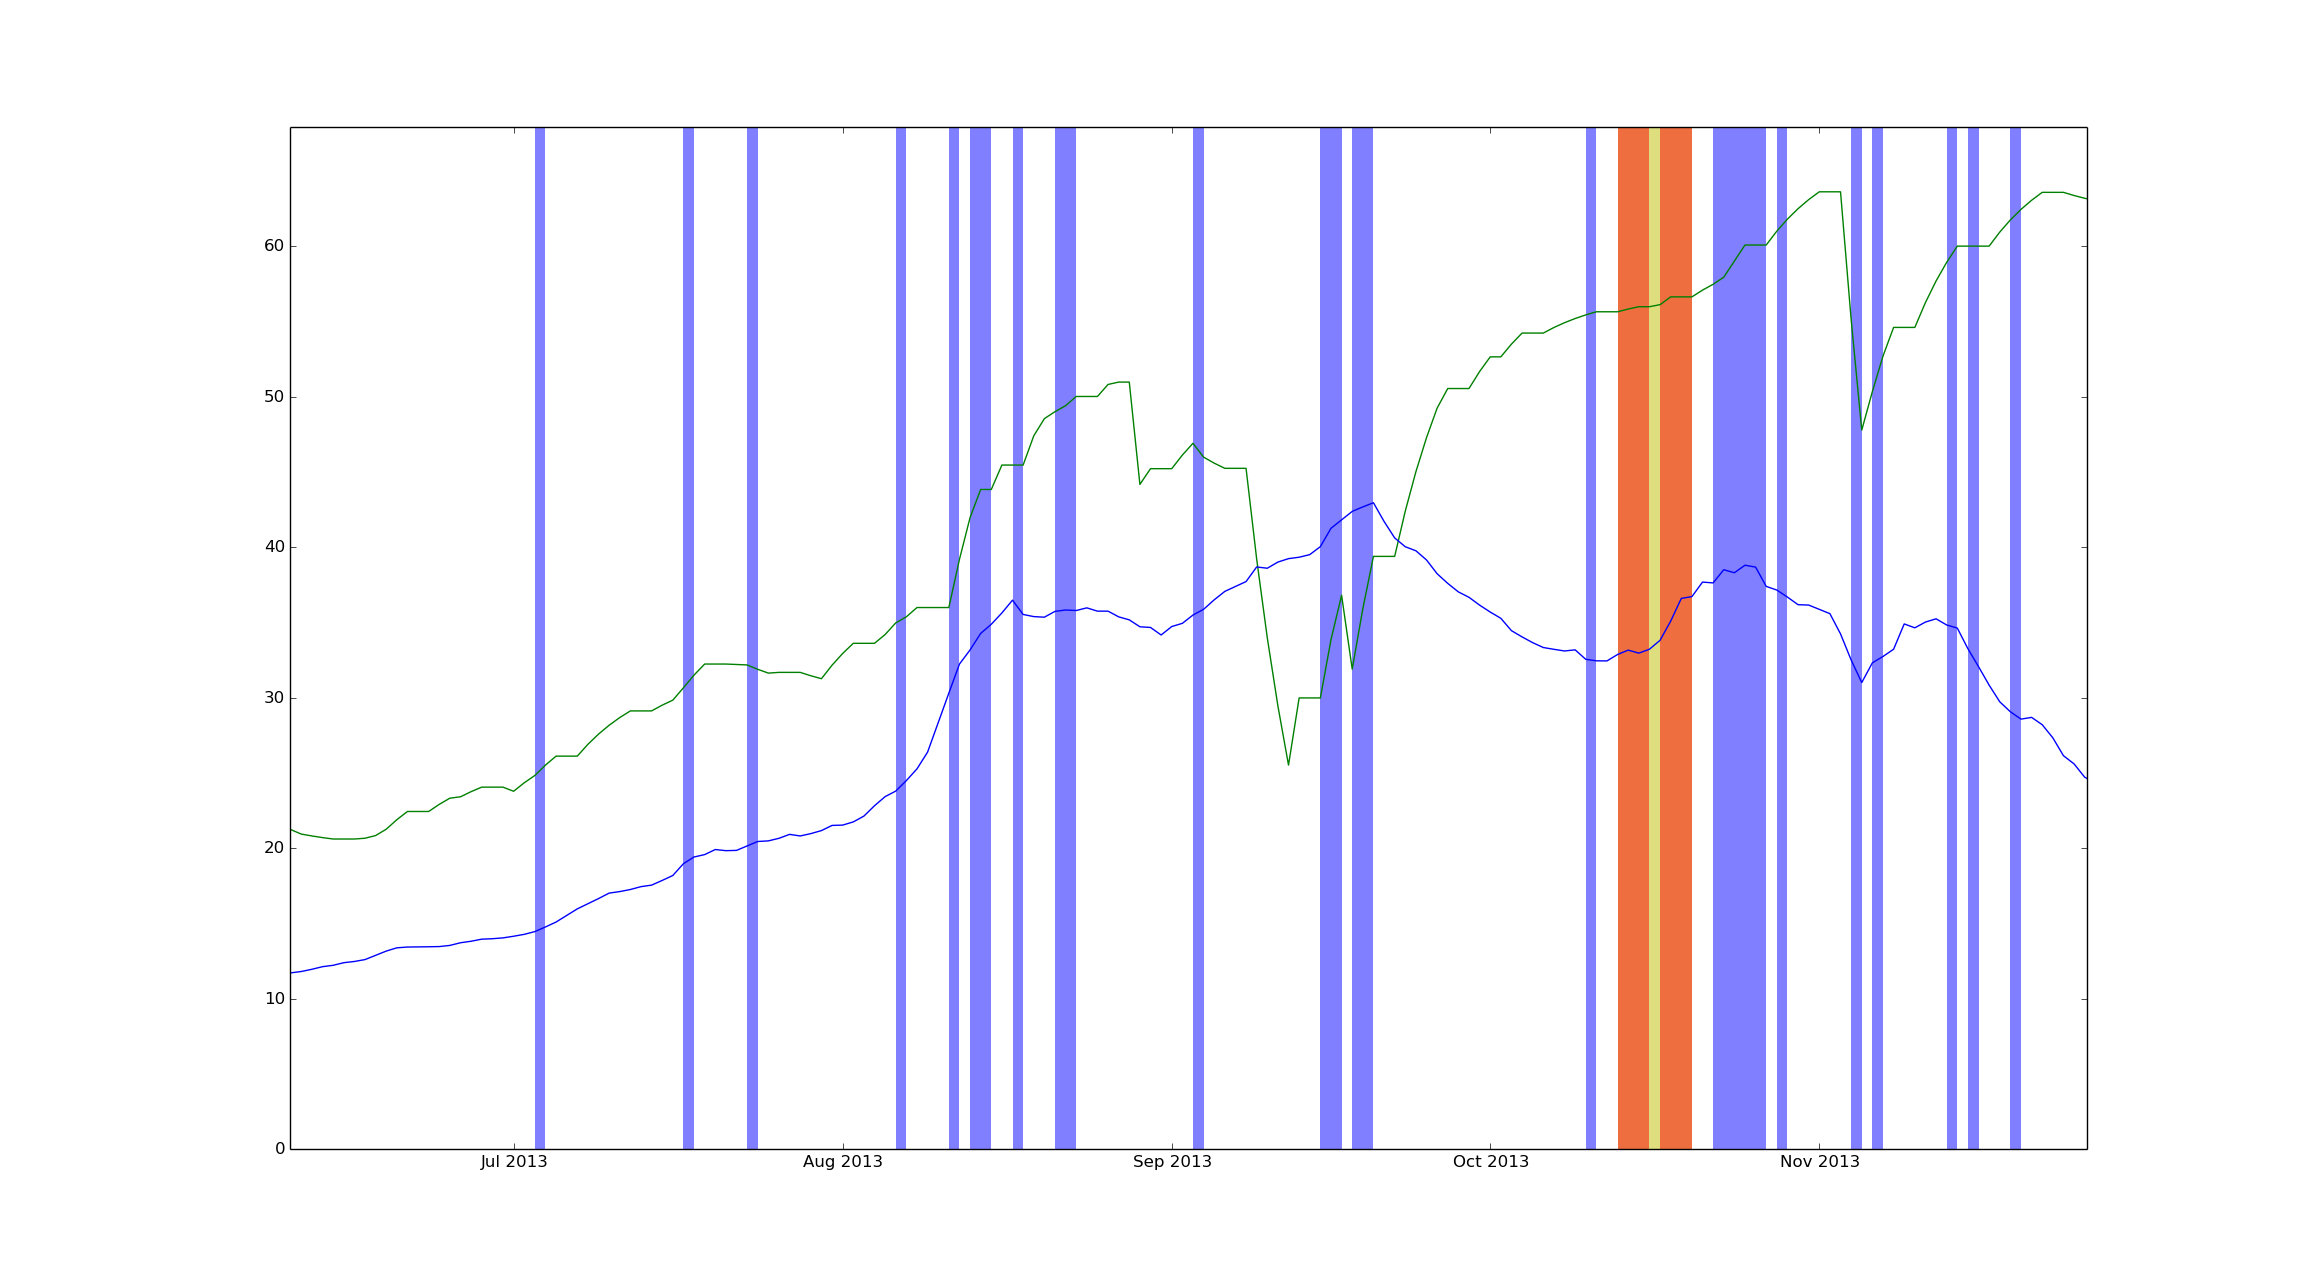
\includegraphics[width=0.8\textwidth]{graphs/12232.png}
		    	\caption{Linear Regression (Green line - Retail Price, Blue Line - Wholesale Price)}
		    	\label{fig:12232}
			\end{figure}
			
					
			
			\item  Note that in the tenure of Oct Nov 2013 (for \textit{Analysis 1}) prices are usually high and as the prices are high, tolerance level also increases little bit. So, even if for some difference it is reported as anomaly at lower price, it is not necessary that for the same difference, it will be reported as anomaly at higher prices. (See Figure \ref{fig:12212})		
			
		\end{itemize}
		
		
		Now we present few observation for Analysis 2 and 4.
		
		
		\begin{itemize}
			\item Here, in this method, it tries to predict what should be retail price or wholesale price based on the arrival of the product. So if the price is too high for the given arrival then it will be reported as anomaly.
			Following tenures are some cases reported by this method:
			\begin{itemize}
				\item \textit{Analysis 2}: Dec 2010, Jan Feb 2011, Aug Sept Oct Nov 2013, Oct Dec 2014 (See Figure \ref{fig:12221})
				\item \textit{Analysis 4}: Dec 2010, July Aug Sept Oct Nov Dec 2013, July 2014 (See Figure \ref{fig:12241})
			\end{itemize}
			\begin{figure}[H]
		    	\centering
  		    	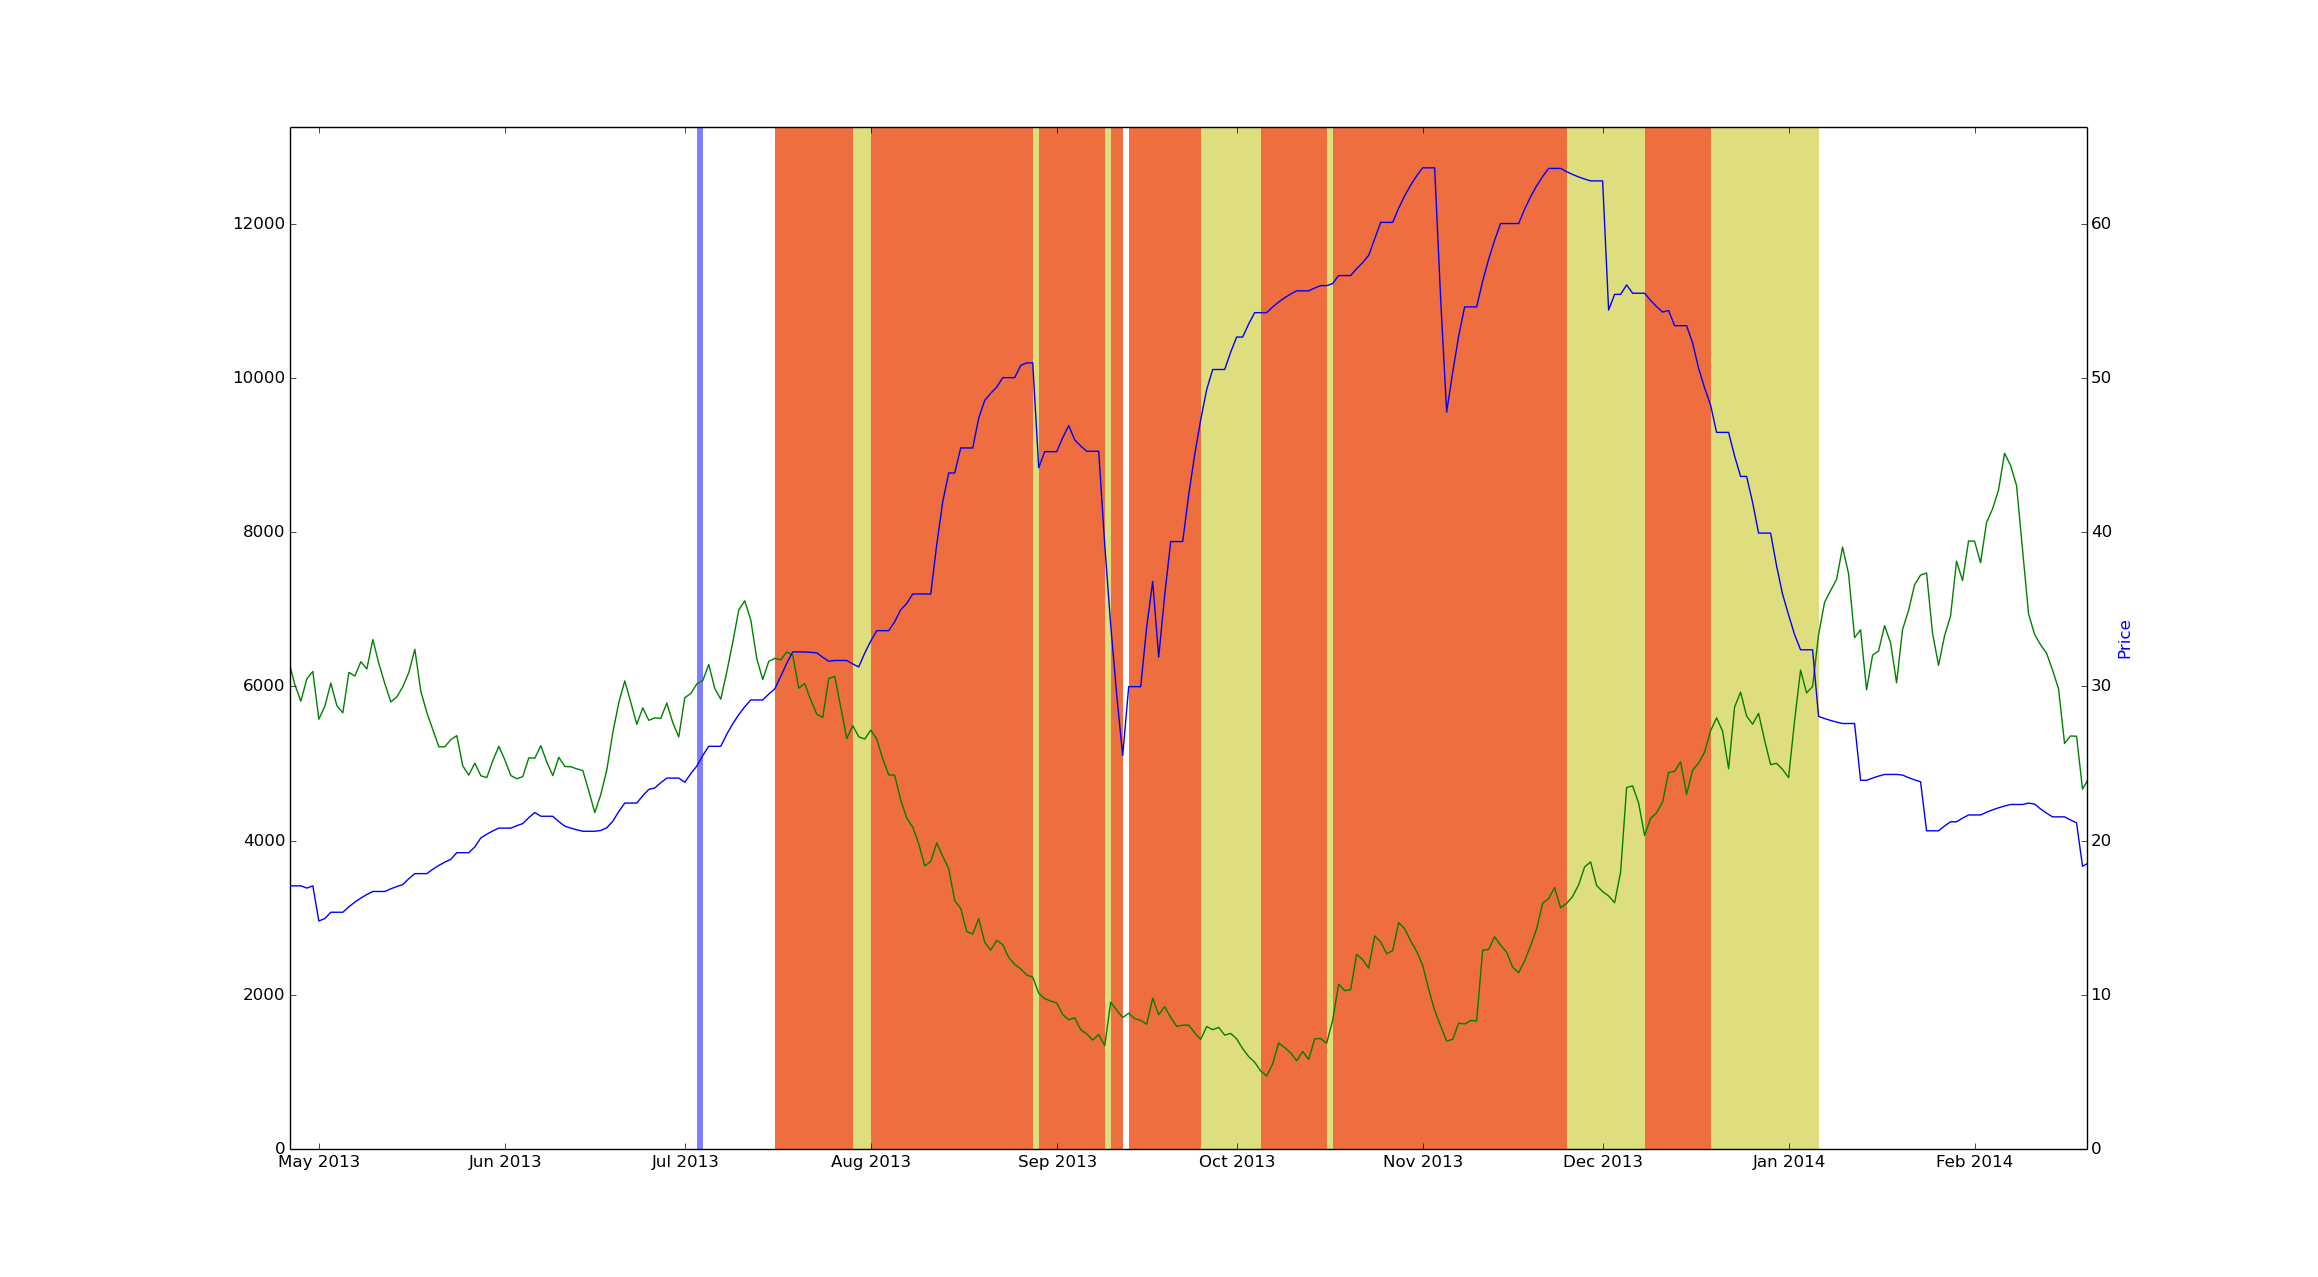
\includegraphics[width=0.8\textwidth]{graphs/12221.png}
		    	\caption{Linear Regression (Green line - Arrival Data of Onion, Blue Line - Retail Price)}
		    	\label{fig:12221}
			\end{figure}
			
			\begin{figure}[H]
		    	\centering
  		    	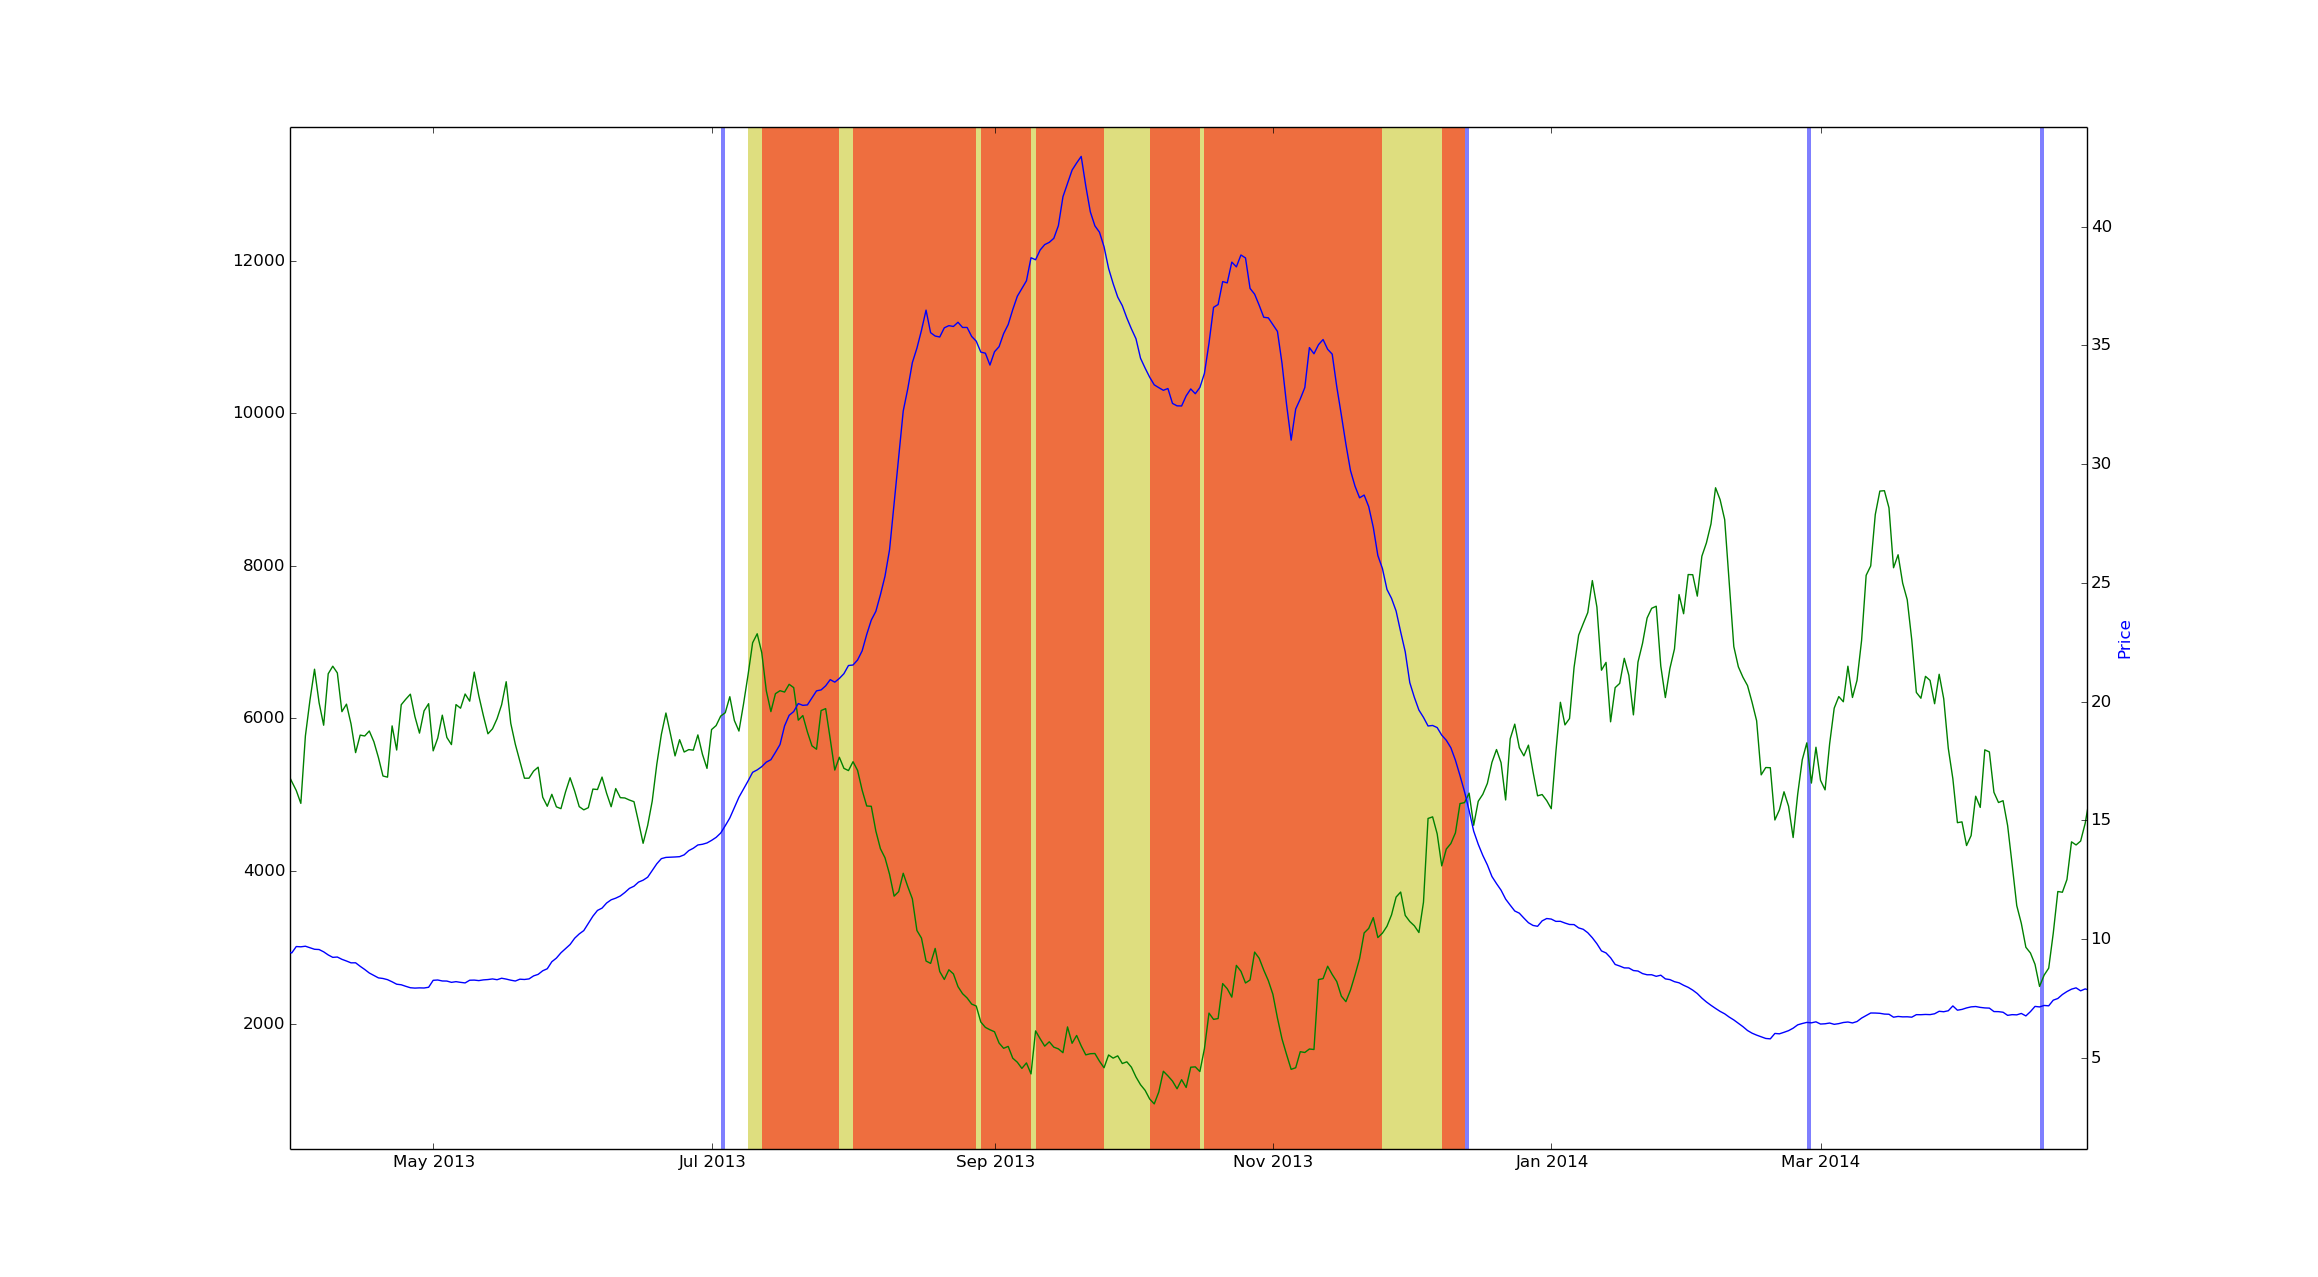
\includegraphics[width=0.8\textwidth]{graphs/12241.png}
		    	\caption{Linear Regression (Green line - Arrival Data of Onion, Blue Line - Wholesale Price)}
		    	\label{fig:12241}
			\end{figure}
			
			
			
			\item Now, this method has also missed few of the articles for this analysis as well. Now, looking at the graphs we could not interpret what may be exact reason why they were missed. But method may have found prices to be moderate and that's why they might have been missed.
			
			Following tenures are some cases reported by this method:
			\begin{itemize}
				\item \textit{Analysis 2}: Jan Feb 2013, July 2014, June July 2015 (See Figure \ref{fig:12222})
				\item \textit{Analysis 4}: Jan Feb 2013, June July 2013, June 2015 (See Figure \ref{fig:12242})
			\end{itemize}
			\begin{figure}[H]
		    	\centering
  		    	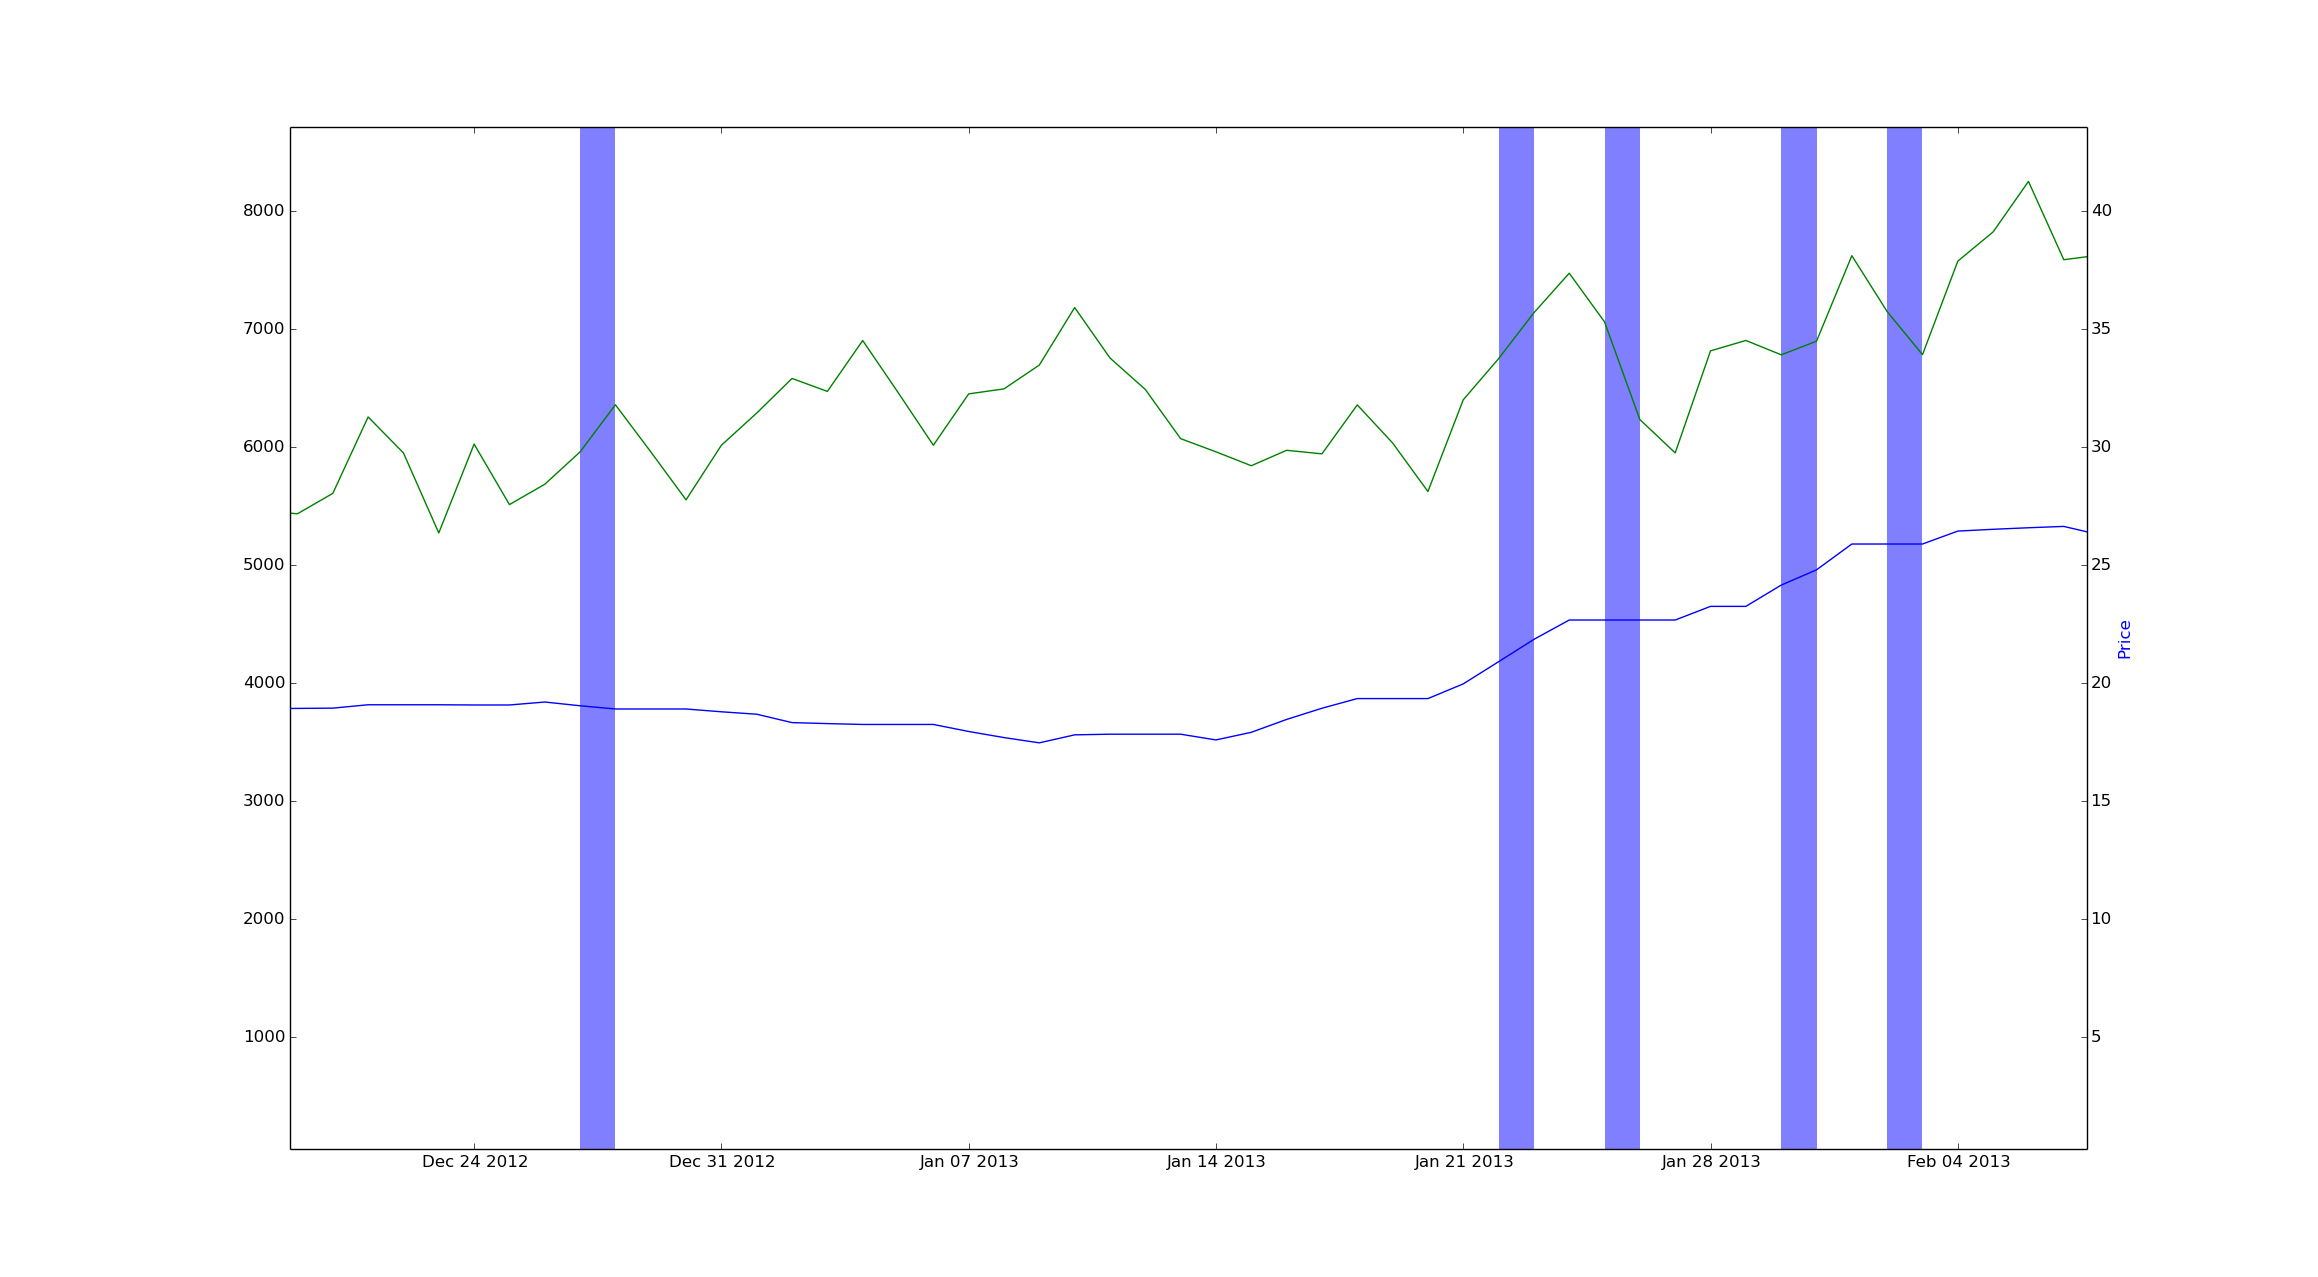
\includegraphics[width=0.8\textwidth]{graphs/12222.png}
		    	\caption{Linear Regression (Green line - Arrival Data of Onion, Blue Line - Retail Price)}
		    	\label{fig:12222}
			\end{figure}
			
			\begin{figure}[H]
		    	\centering
  		    	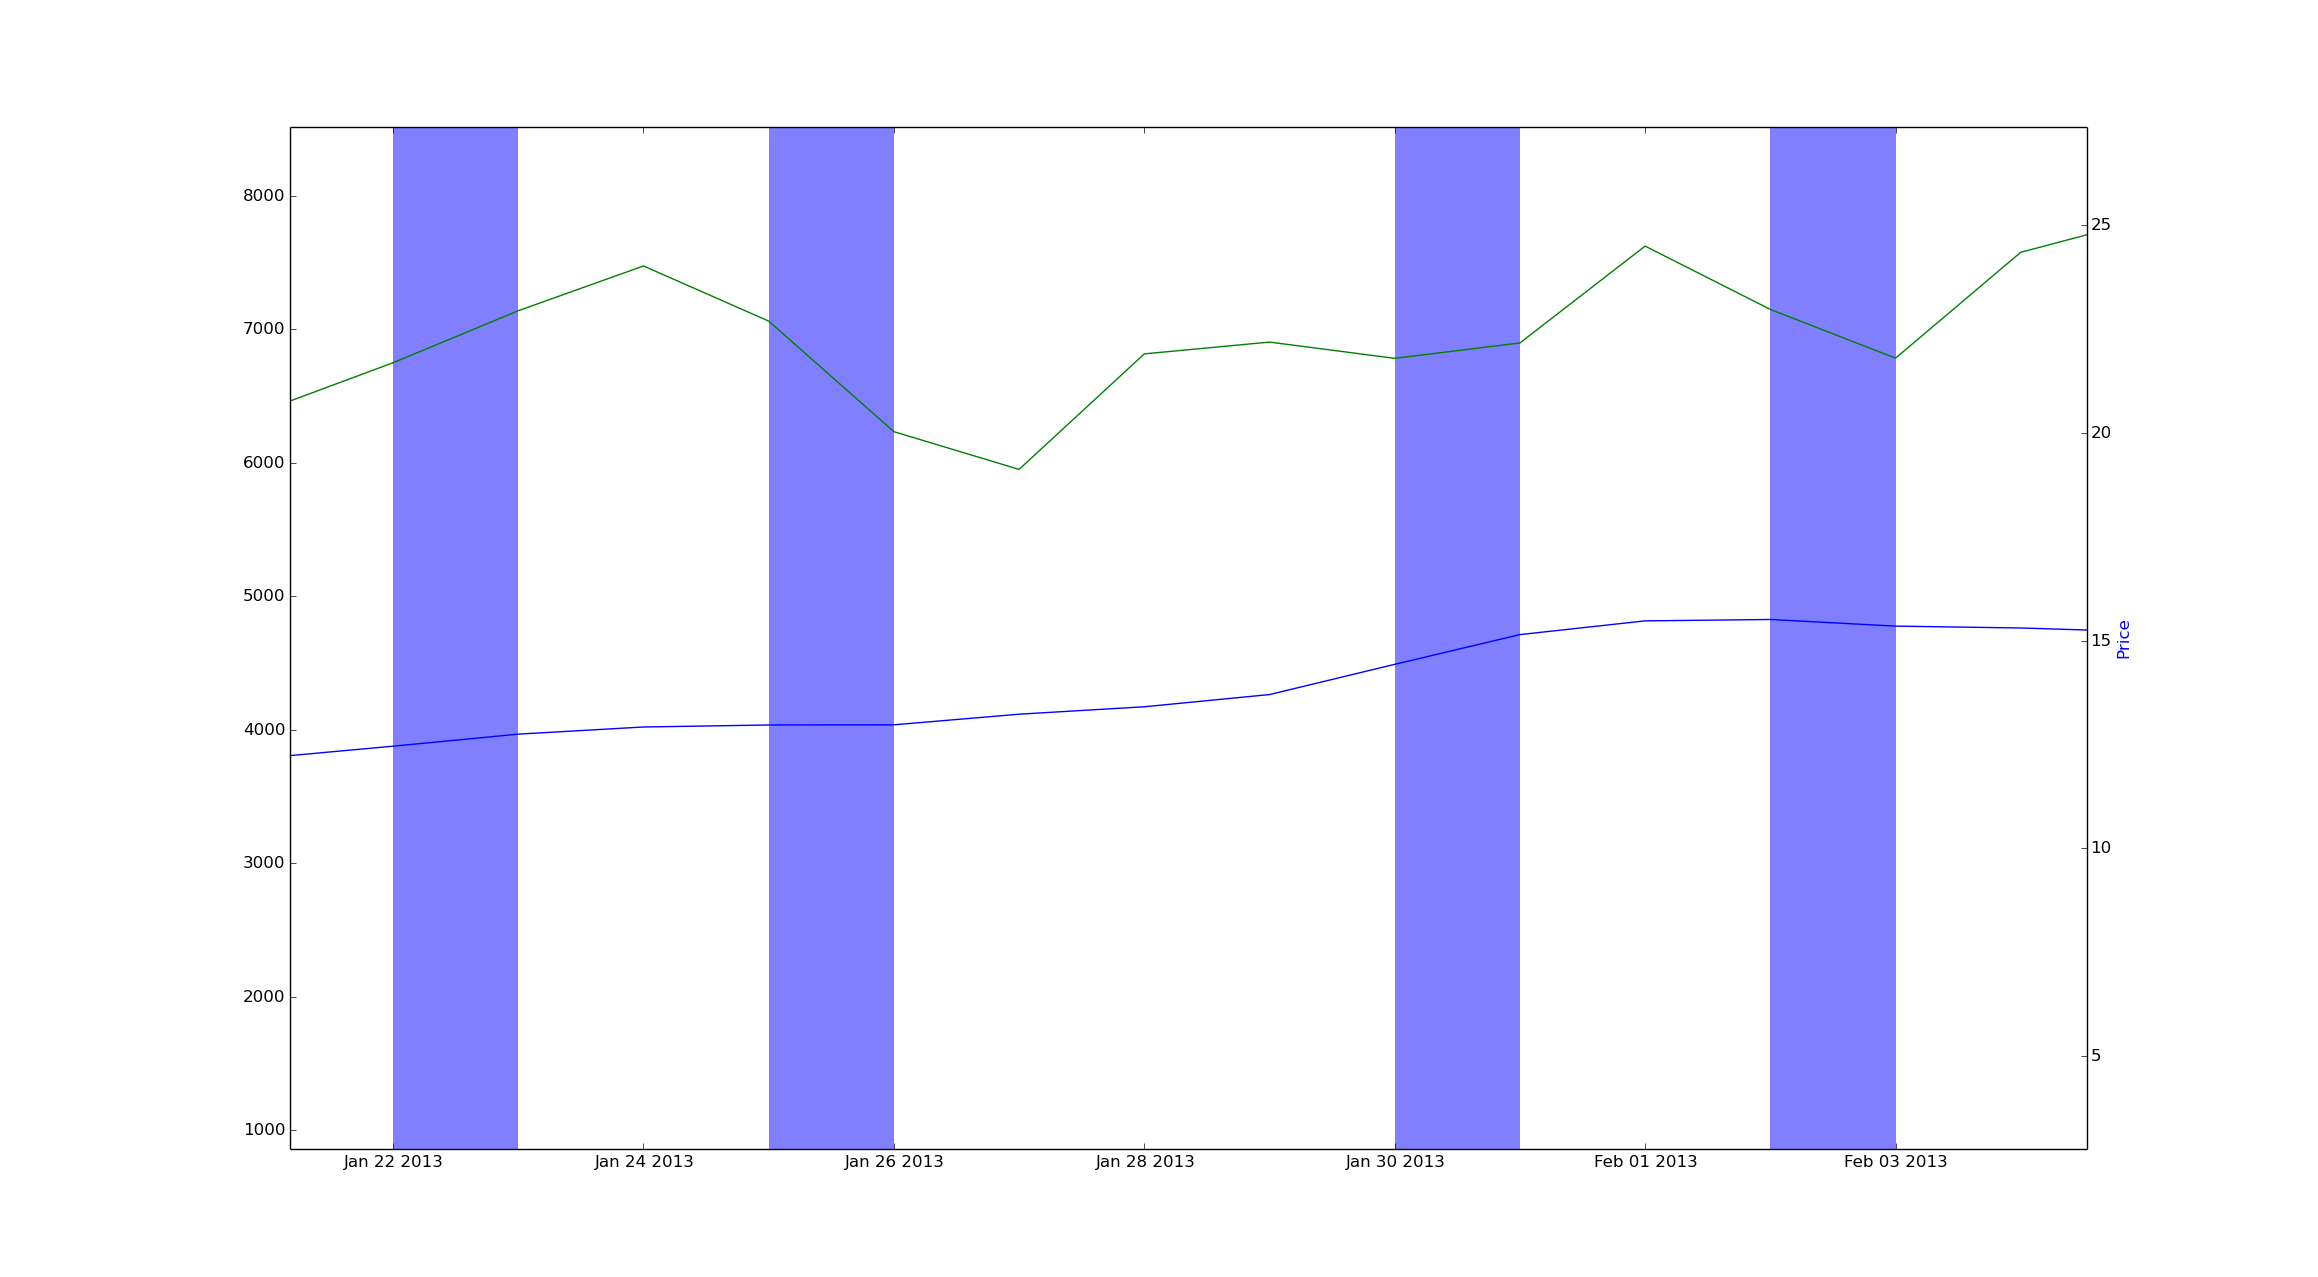
\includegraphics[width=0.8\textwidth]{graphs/12242.png}
		    	\caption{Linear Regression (Green line - Arrival Data of Onion, Blue Line - Wholesale Price)}
		    	\label{fig:12242}
			\end{figure}
		\end{itemize}

		
\subsection{Window Based Correlation}

		This method checks if the provided two timeseries moves in tandem or not. If not, then what are the time periods when they are not following the desired behavior. In order to find such time periods in the timeseries, the whole timeseries is divided into smaller windows and correlation value computed for that window is used to determine if that period is anomalous or not. The P-value of 0.01 is used in order to check the significance of correlation value.
		\\
		\\
		The function is tested with different set of timeseries. Following are the four tests which were performed:
		\begin{enumerate}
			\item \textbf{Retail Price vs Average of Retail Price}: This test tries to find if any centre deviates from other centres abruptly. Average of timeseries of all the centres is taken as a representative timeseries for the behavior of all the centres which is compared with every centre in order to find time periods where these two did not move in tandem
			\item \textbf{Retail Price vs Arrival of Onion}: Retail timeseries is expected not to move in tandem with Arrival timeseries. So, the time periods with positive correlation values are spotted in this. 
			\item \textbf{Retail Price vs Wholesale Price}: Retail timeseries is expected to move in tandem with wholesale timeseries. So, the time periods with negative correlation values are spotted in this.
			\item \textbf{Wholesale Price vs Arrival of Onion}: Wholesale timeseries is expected to not move in tandem with Arrival timeseries. So, the time periods with positive correlation values are spotted in this. 
		\end{enumerate}
		
		The two timeseries are first aligned with each other at the maximum lag value. Then the entire timeseries is divided into small time periods of 15 days in order to locate anomalous situations through their respective correlation values.
		\\
		\\
		Observations when retail price timeseries is compared with average of retail price timeseries: 
		
		\begin{itemize}
			\item The timeseries showed the initial shift/lag of zero days which means both the timeseries are best aligned without any lag.
			
			Some of the tenures for which the method reported anomalies are:
			
			\begin{itemize}
				\item 2008-03-06 to 2008-03-20 (See Figure \ref{fig:20080306_0320})
				\item 2009-09-12 to 2009-09-26 (See Figure \ref{fig:20090912_0926})
				\item 2011-07-04 to 2011-08-02 (See Figure \ref{fig:20110704_0802})
			\end{itemize}
			\begin{figure}[H]
		    	\centering
  		    	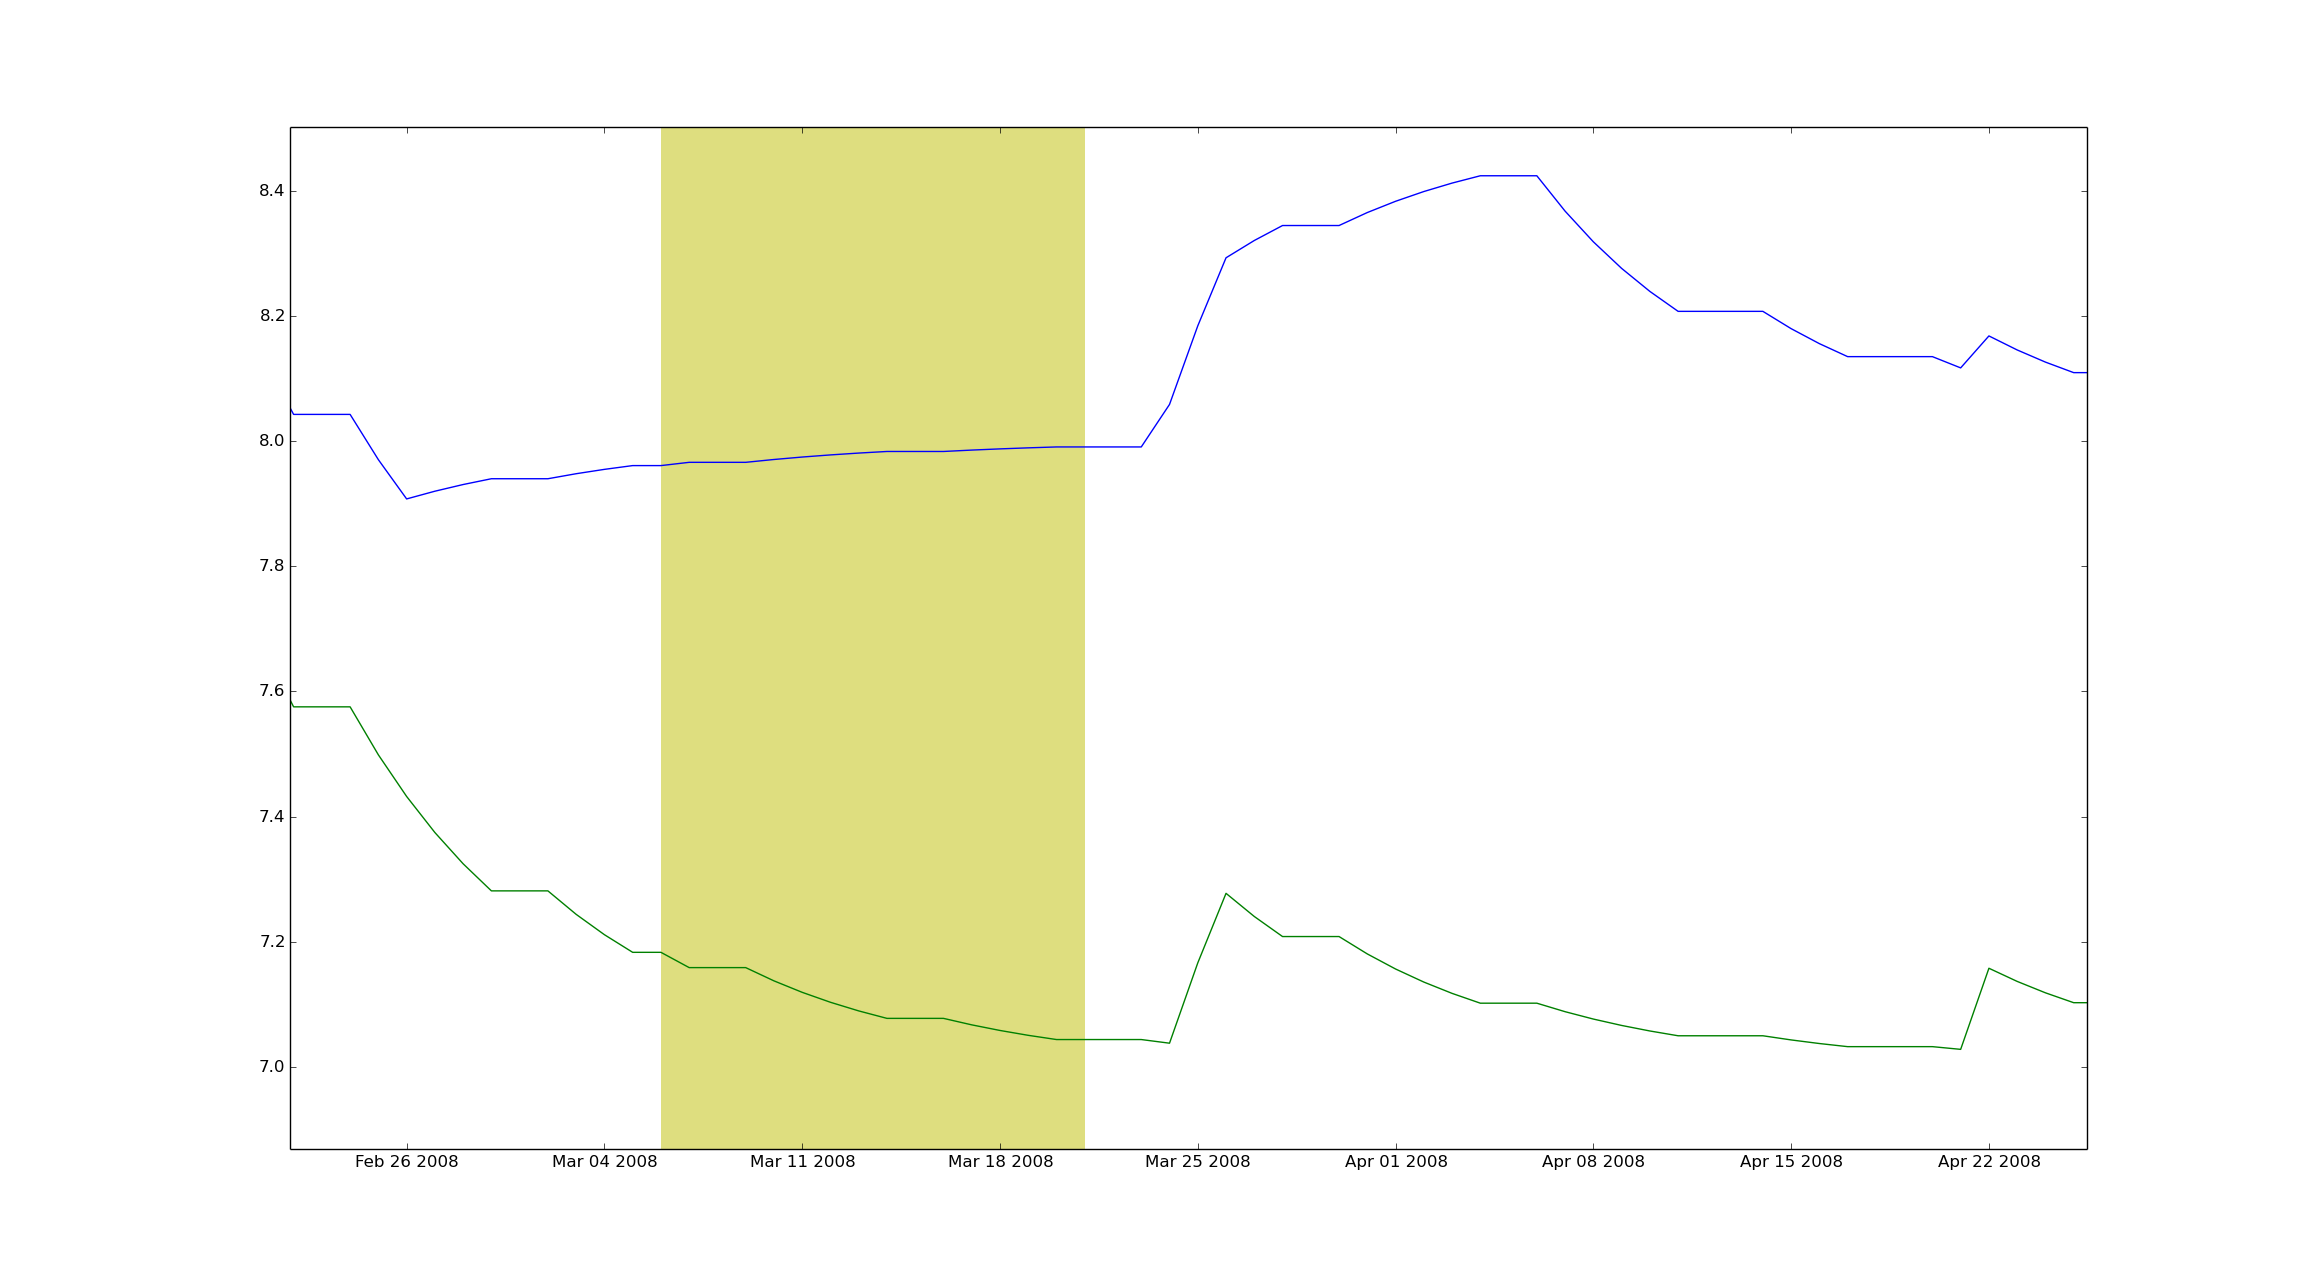
\includegraphics[width=0.8\textwidth]{graphs/20080306_0320.png}
		    	\caption{Window based correlation (Green line - Centre Retail Price, Blue Line - Average Retail Price)}
		    	\label{fig:20080306_0320}
			\end{figure}
			
			\begin{figure}[H]
		    	\centering
  		    	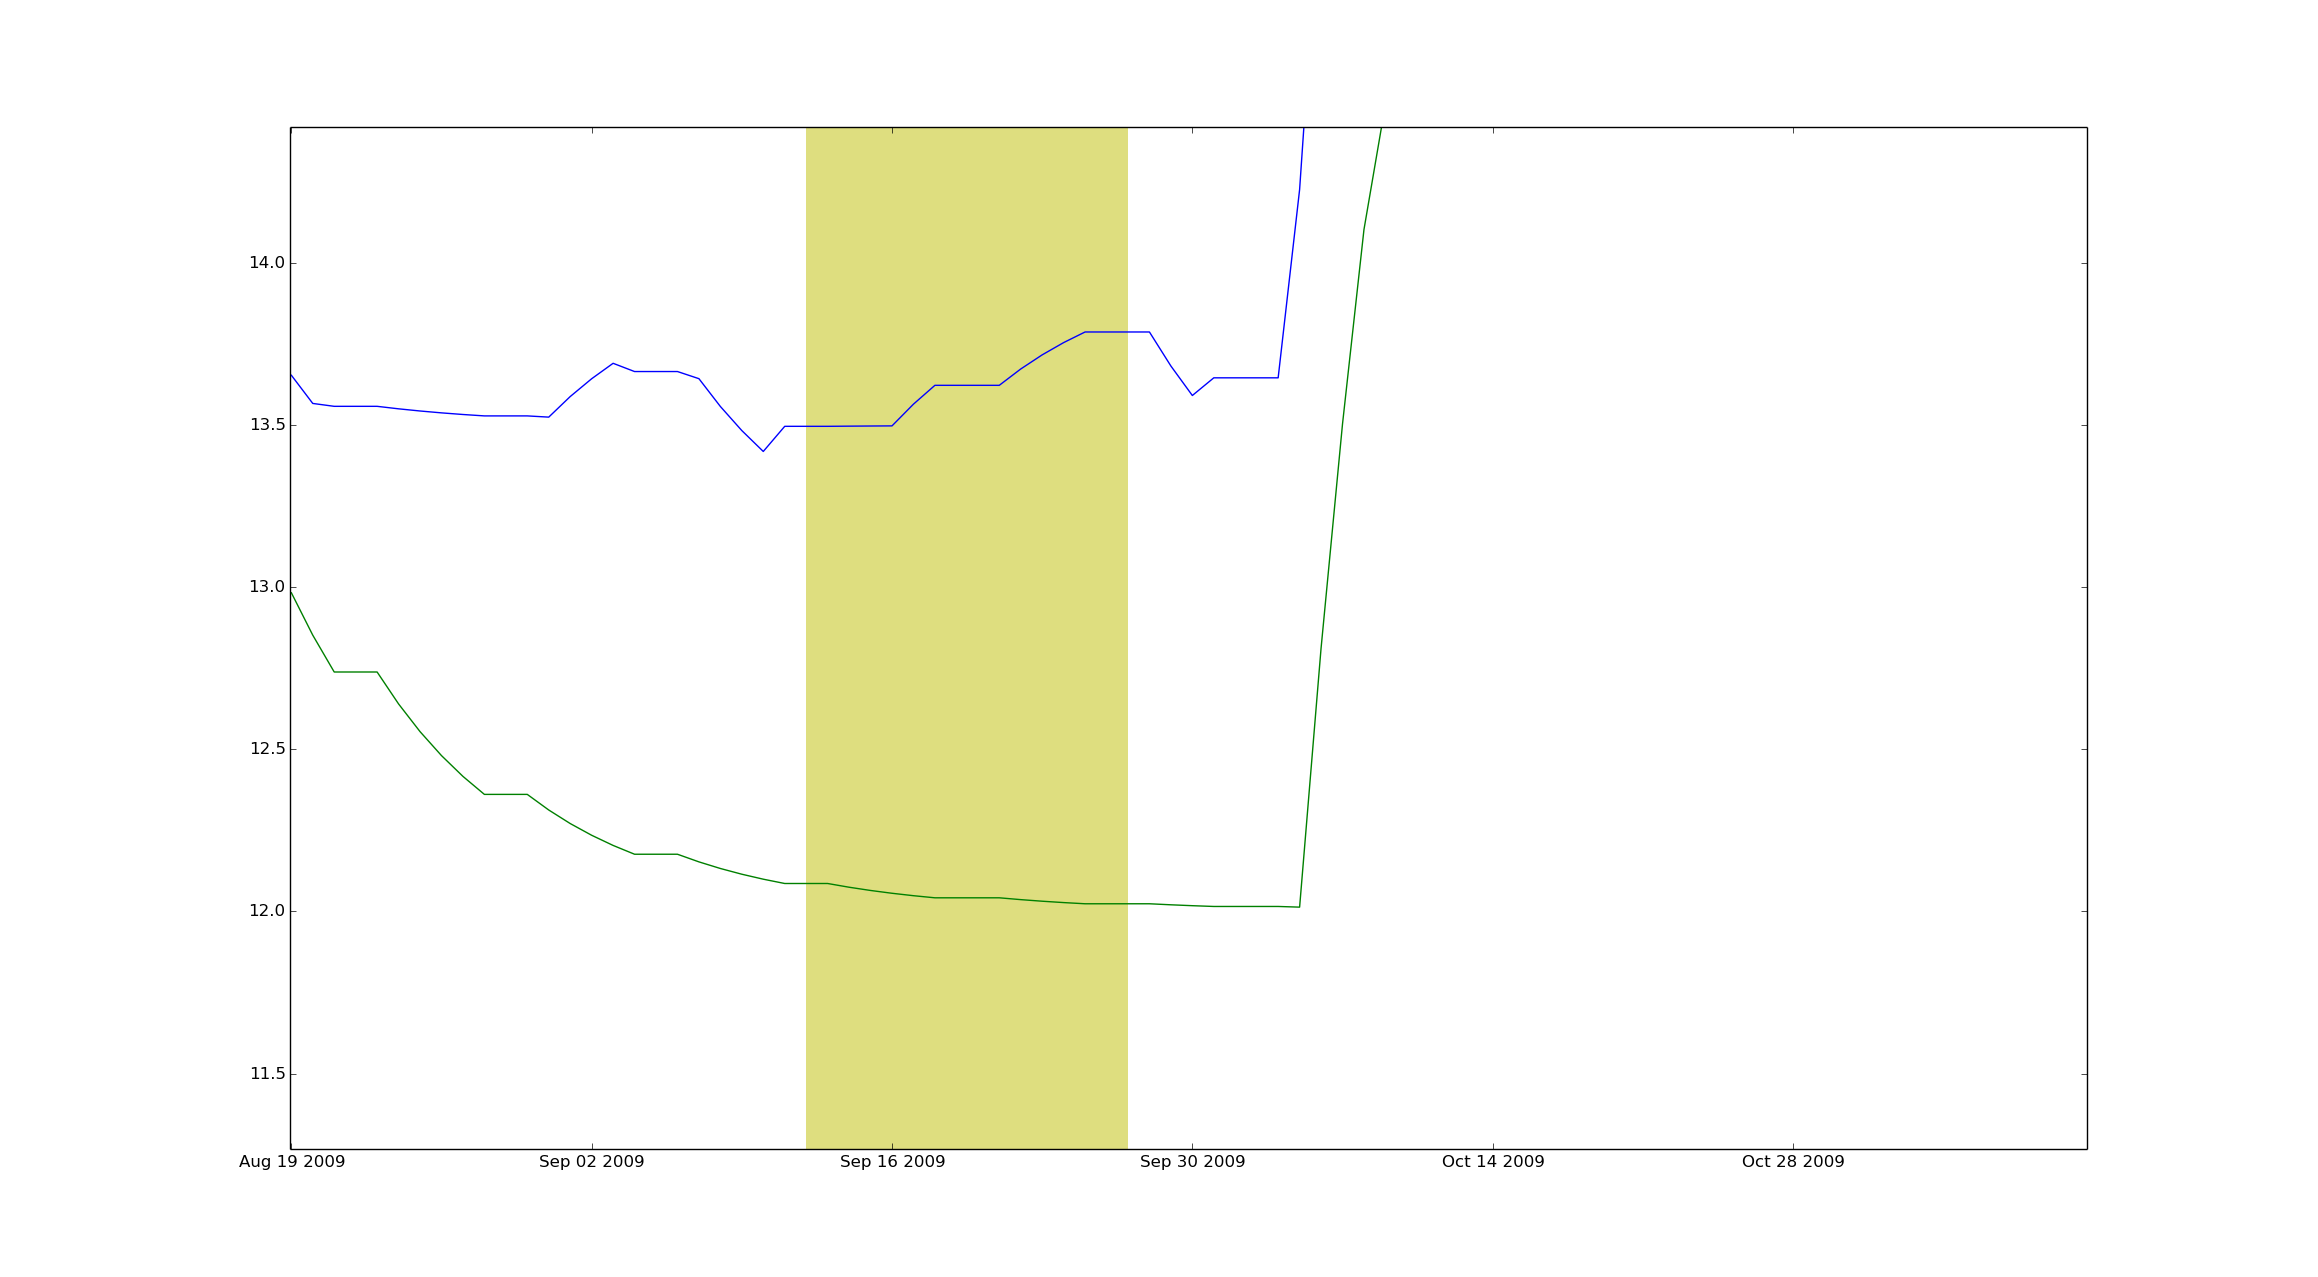
\includegraphics[width=0.8\textwidth]{graphs/20090912_0926.png}
		    	\caption{Window based correlation (Green line - Centre Retail Price, Blue Line - Average Retail Price)}
		    	\label{fig:20090912_0926}
			\end{figure}

			\begin{figure}[H]
		    	\centering
  		    	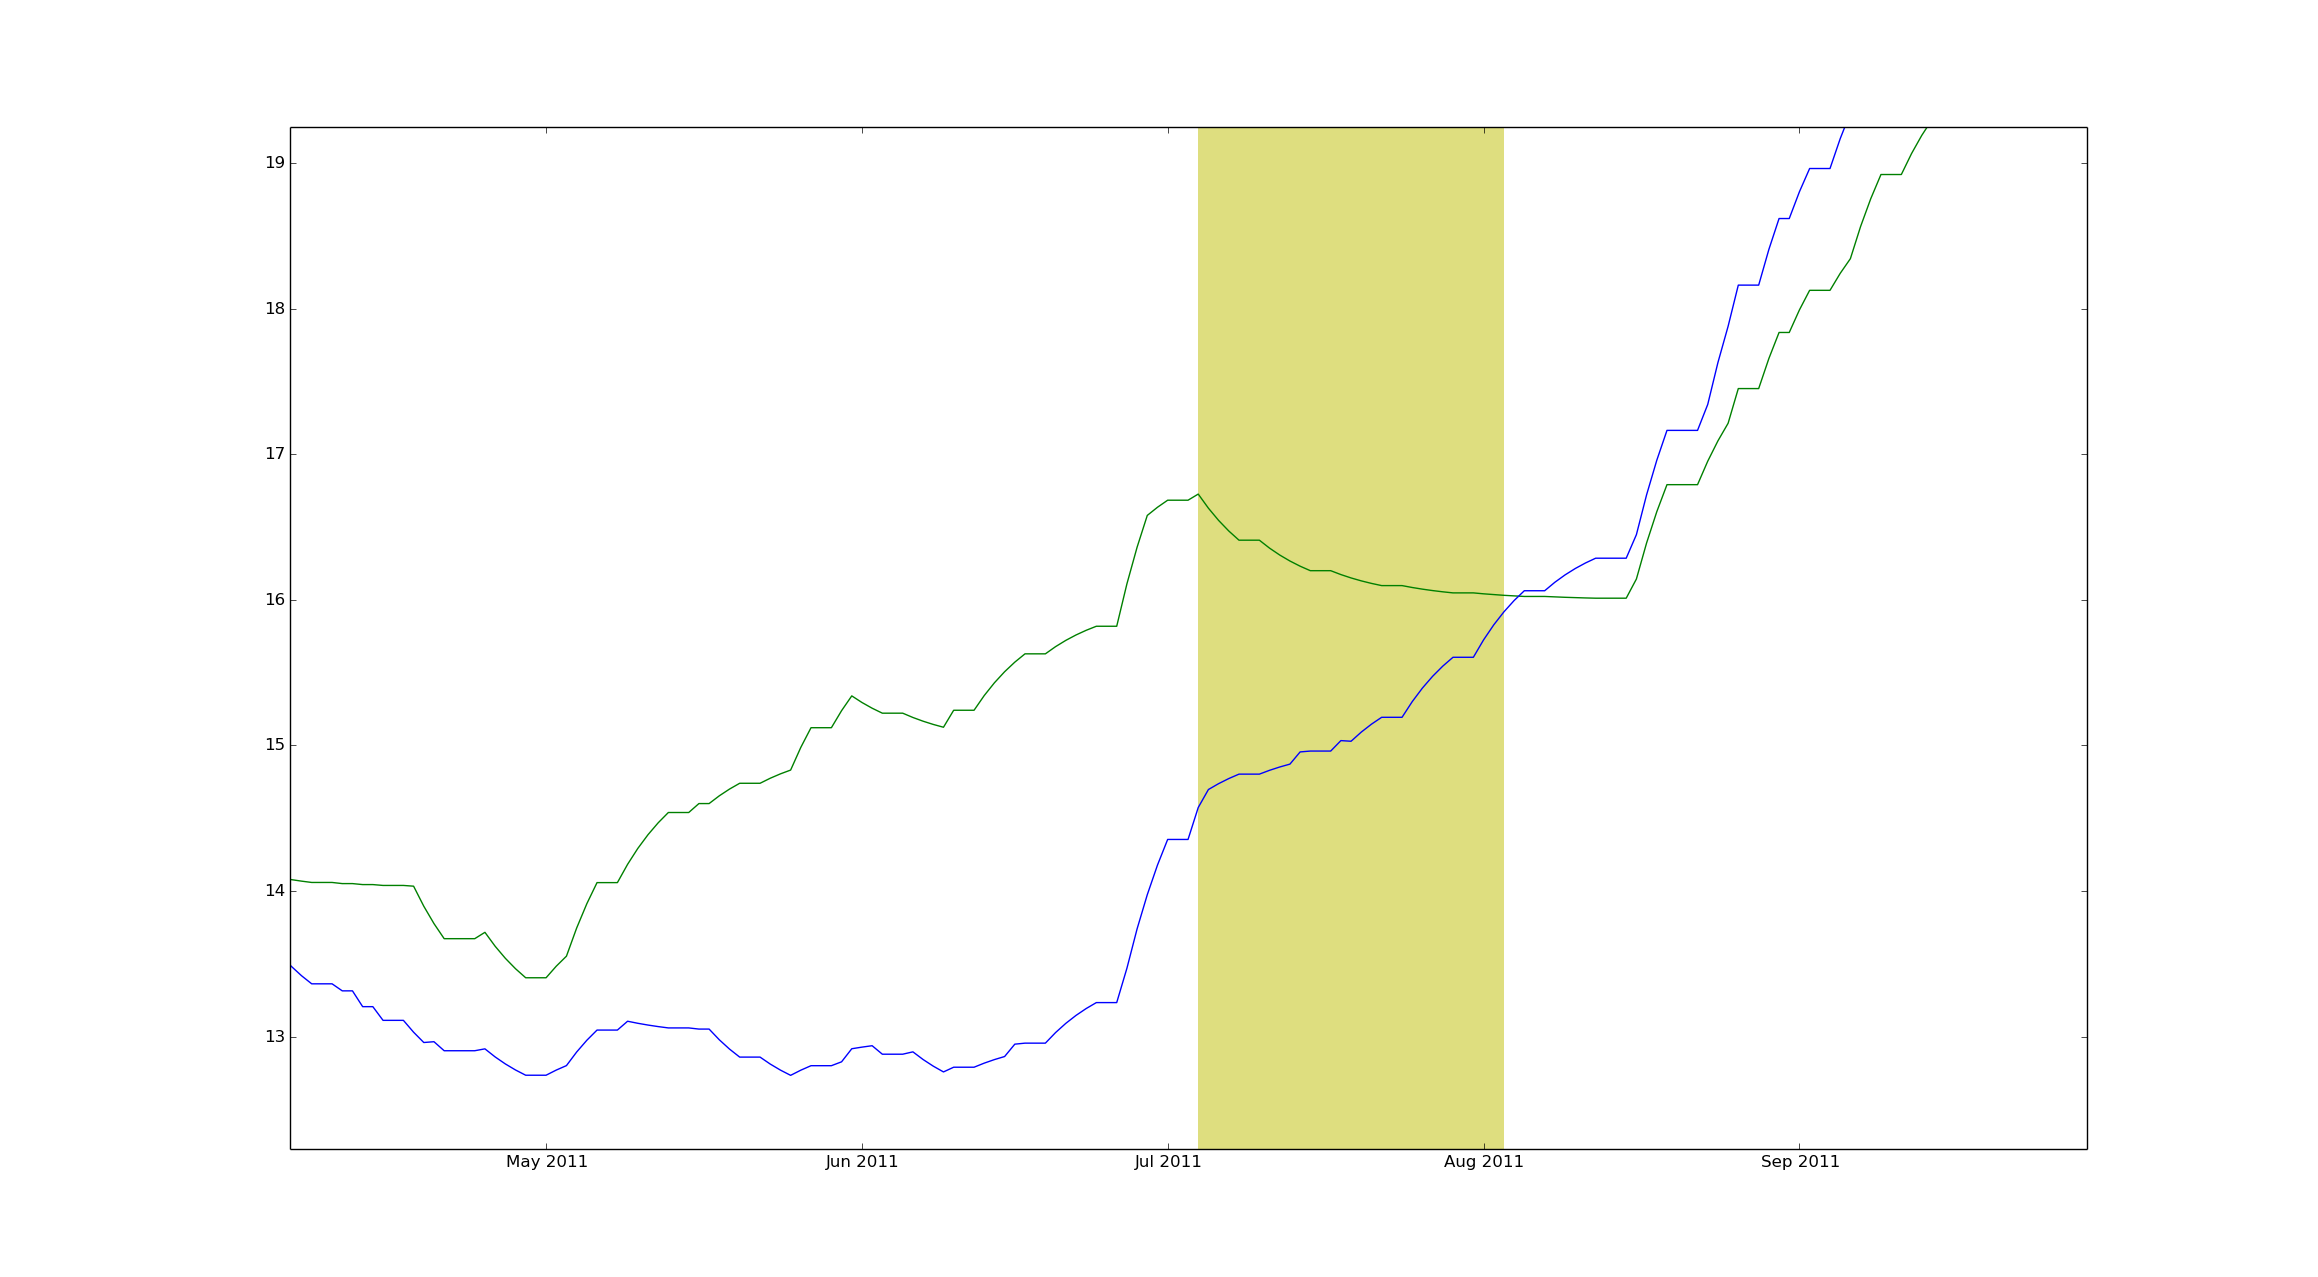
\includegraphics[width=0.8\textwidth]{graphs/20110704_0802.png}
		    	\caption{Window based correlation (Green line - Centre Retail Price, Blue Line - Average Retail Price)}
		    	\label{fig:20110704_0802}
			\end{figure}
			
			But looking closely in the data, it is found that these tenures are reported because the two series were not in tandem which was mostly because prices of delhi faced some fluctuations whereas Mumbai prices did not show evident fluctuations. One of the reason for fluctuation in prices of Delhi over Mumbai could be because Delhi is dependent on other states for Onion whereas Mumbai does not have such issue.
			\\
			\\
			Some of the tenures which went unnoticed by method:
			
			\begin{itemize}
				\item 2010-12-20 to 2010-12-25 (See Figure \ref{fig:20101220_1225})
				\item 2011-01-06 to 2011-01-08 (See Figure \ref{fig:20110106_0108})
				\item 2012-12-27 to 2013-01-05 (See Figure \ref{fig:20121227_0105})
			\end{itemize}
			\begin{figure}[H]
		    	\centering
  		    	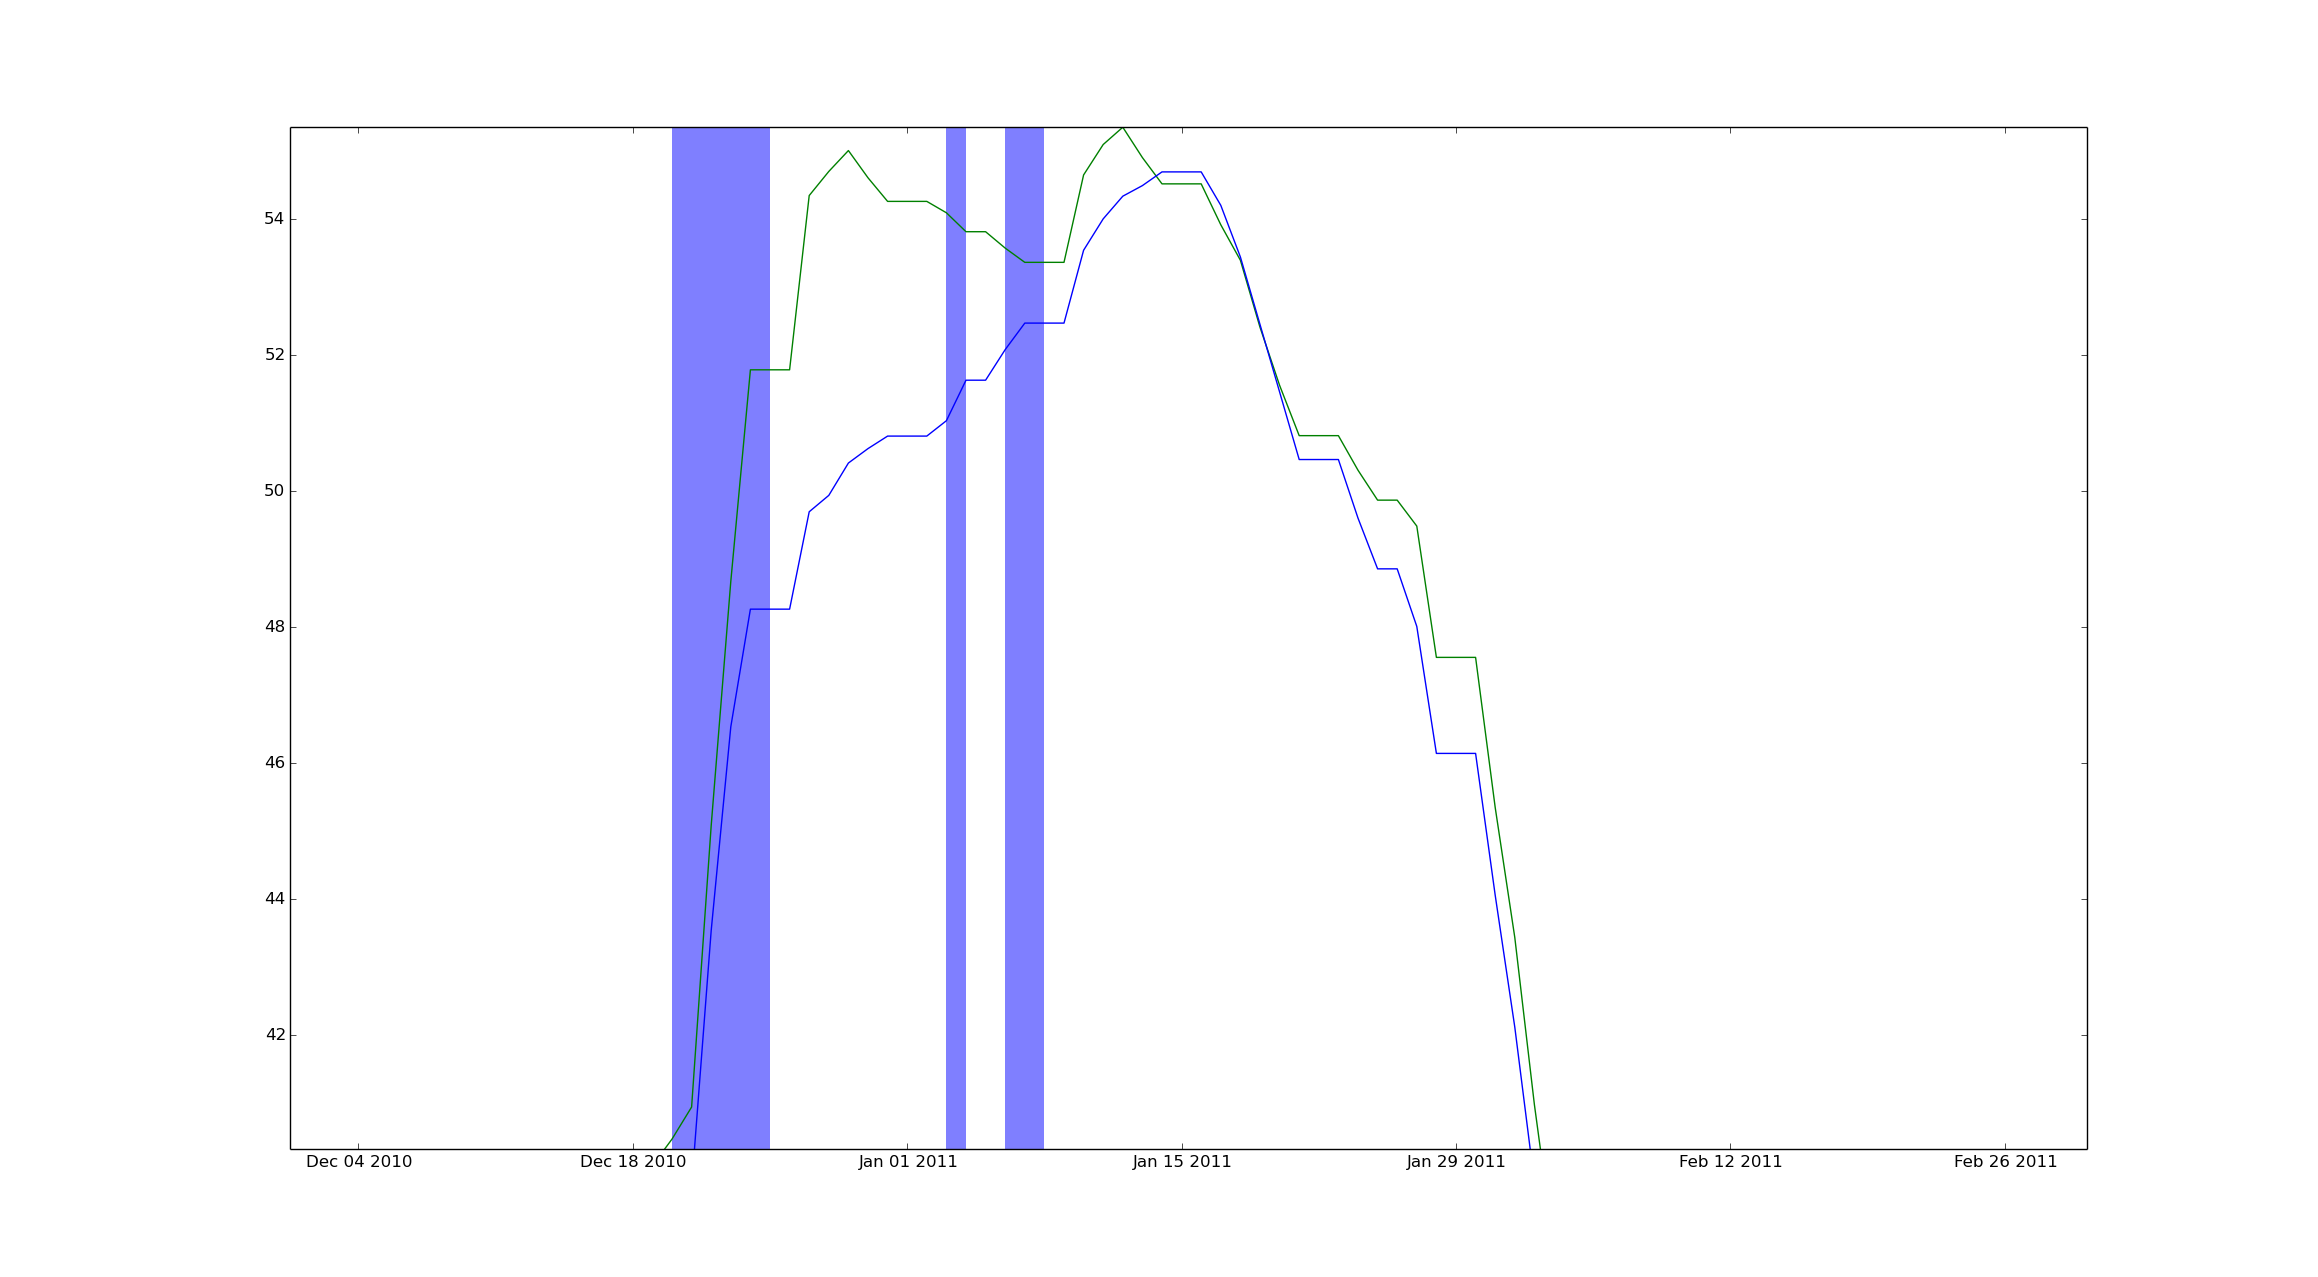
\includegraphics[width=0.8\textwidth]{graphs/20101220_1225.png}
		    	\caption{Window based correlation (Green line - Centre Retail Price, Blue Line - Average Retail Price)}
		    	\label{fig:20101220_1225}
			\end{figure}
			
			\begin{figure}[H]
		    	\centering
  		    	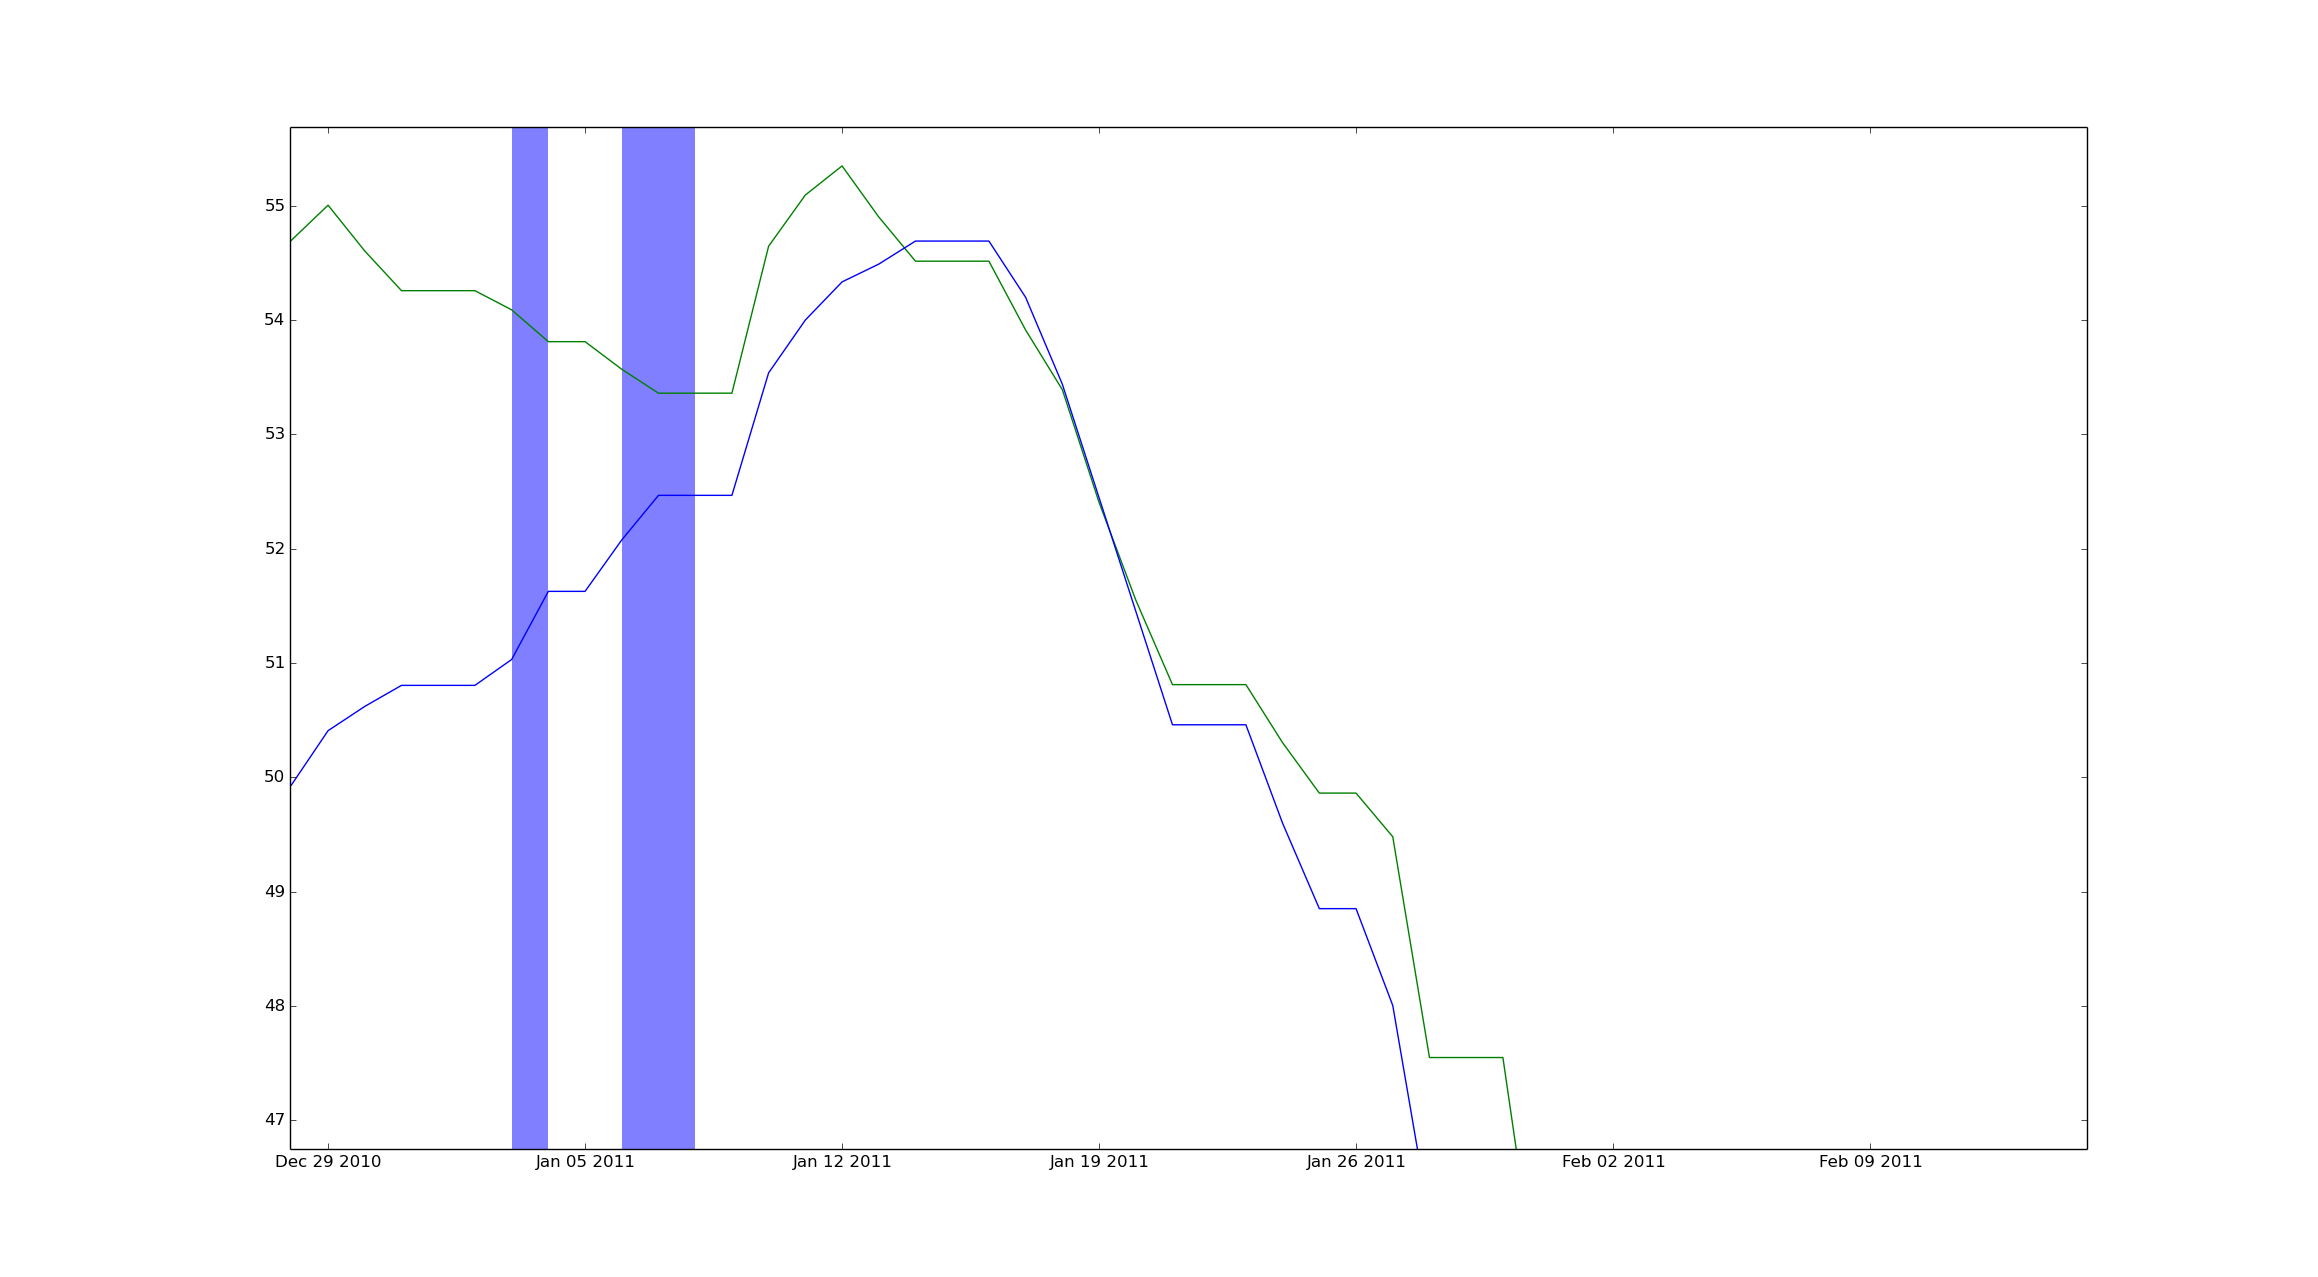
\includegraphics[width=0.8\textwidth]{graphs/20110106_0108.png}
		    	\caption{Window based correlation (Green line - Centre Retail Price, Blue Line - Average Retail Price)}
		    	\label{fig:20110106_0108}
			\end{figure}

			\begin{figure}[H]
		    	\centering
  		    	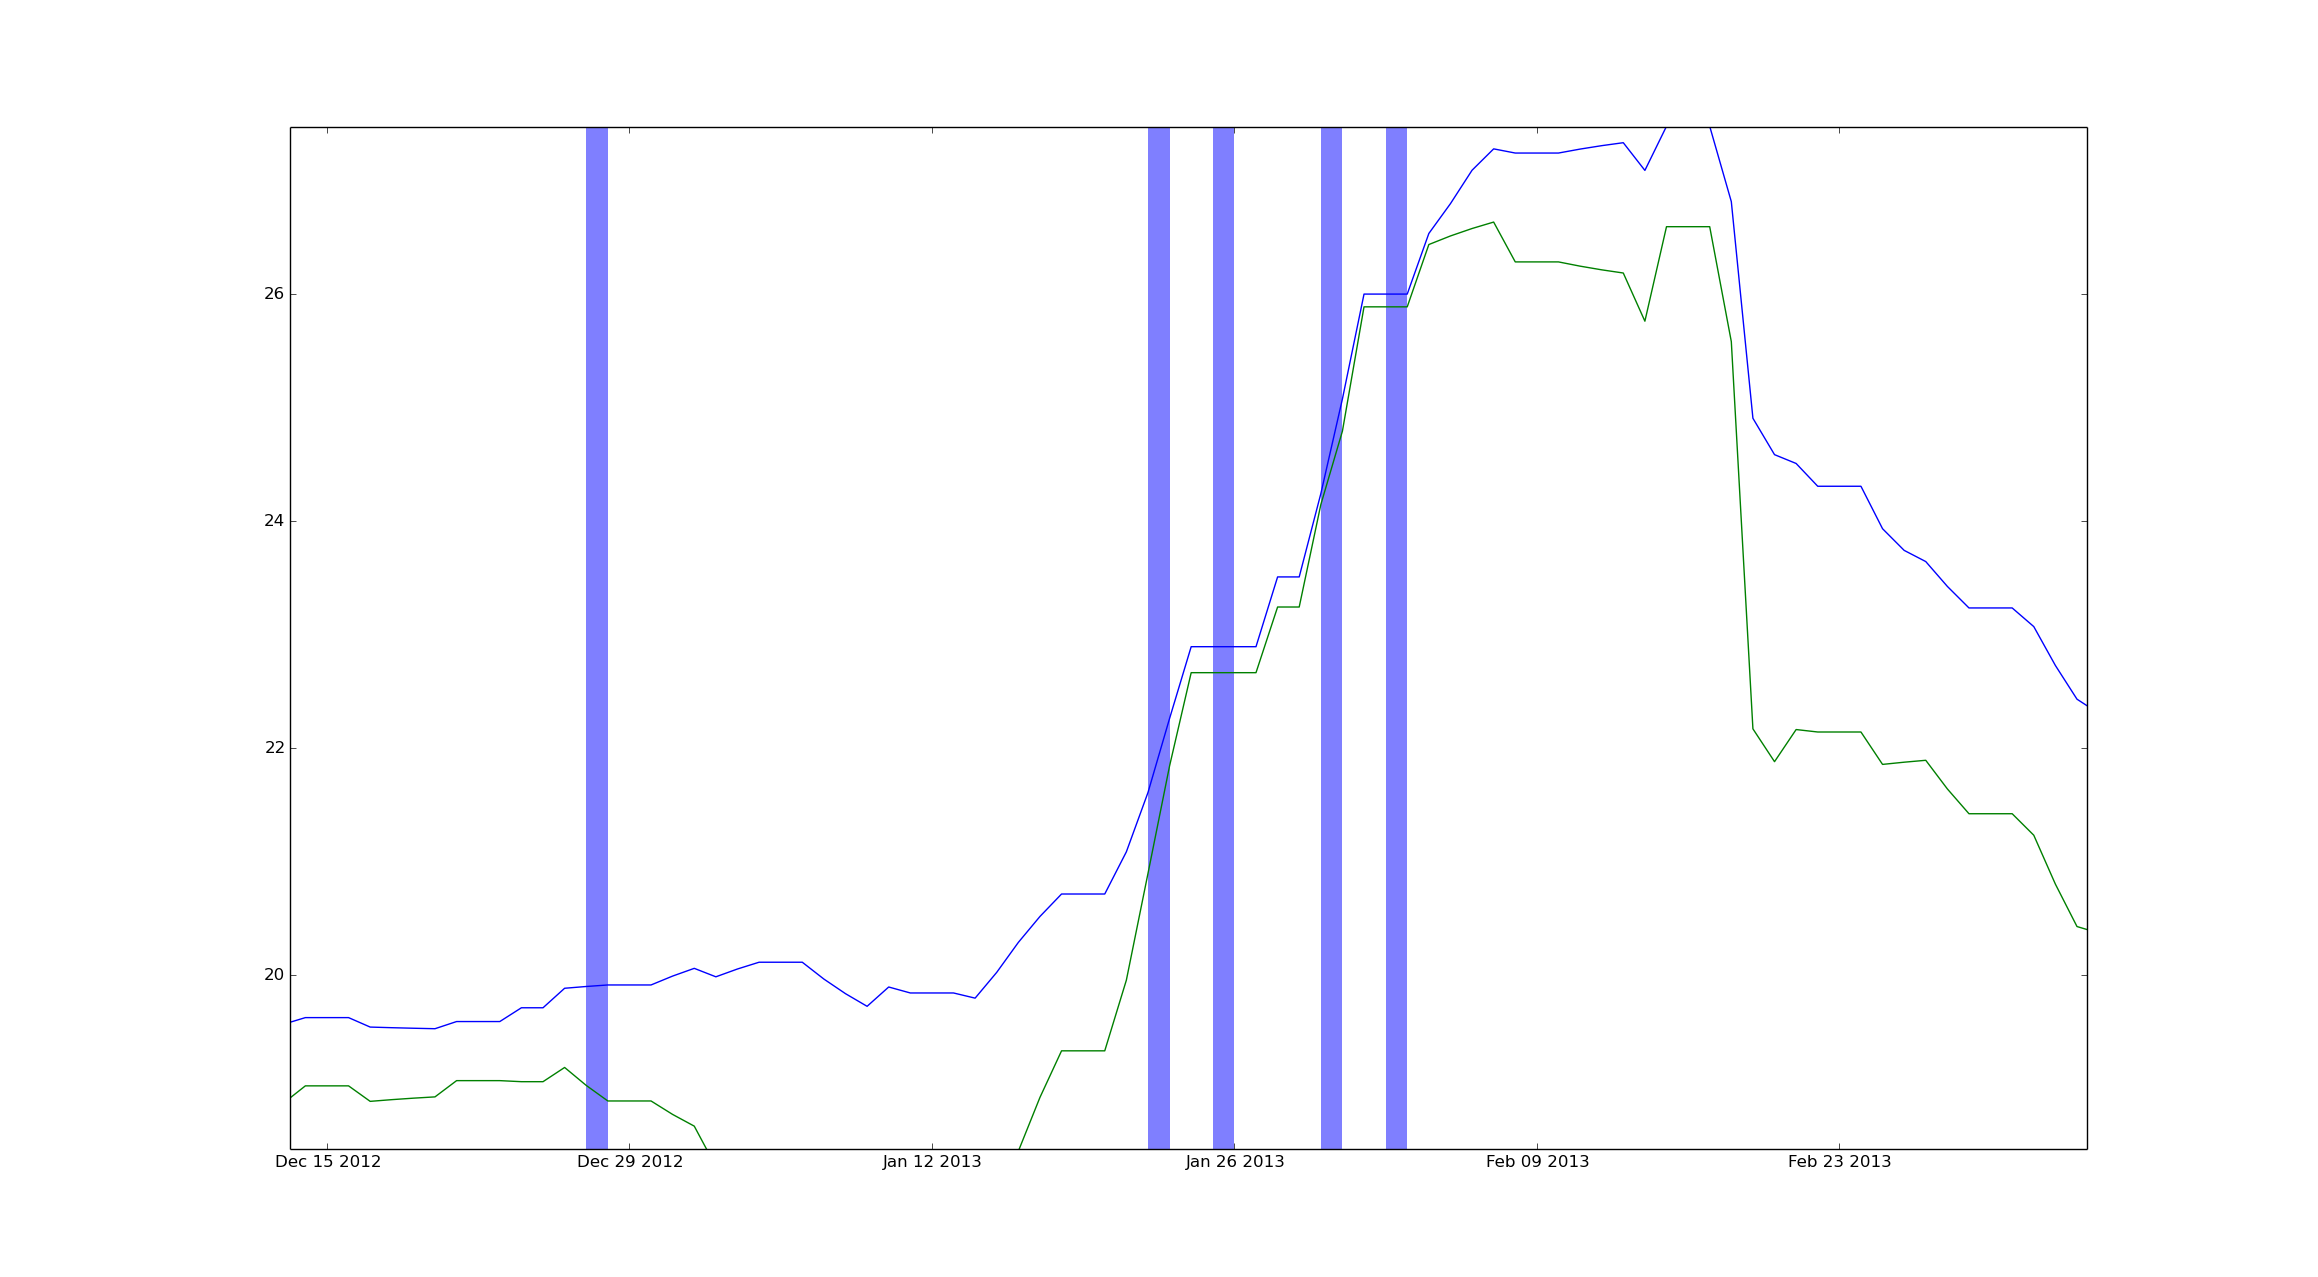
\includegraphics[width=0.8\textwidth]{graphs/20121227_0105.png}
		    	\caption{Window based correlation (Green line - Centre Retail Price, Blue Line - Average Retail Price)}
		    	\label{fig:20121227_0105}
			\end{figure}
			
			Some of the tenures which were reported by news reports as well as method:
			
			\begin{itemize}
				\item 2013-10-06 to 2013-10-15 (See Figure \ref{fig:20131006_1015_1021})
				\item 2013-10-17 to 2013-10-21 (See Figure \ref{fig:20131006_1015_1021})
			\end{itemize}
			\begin{figure}[H]
		    	\centering
  		    	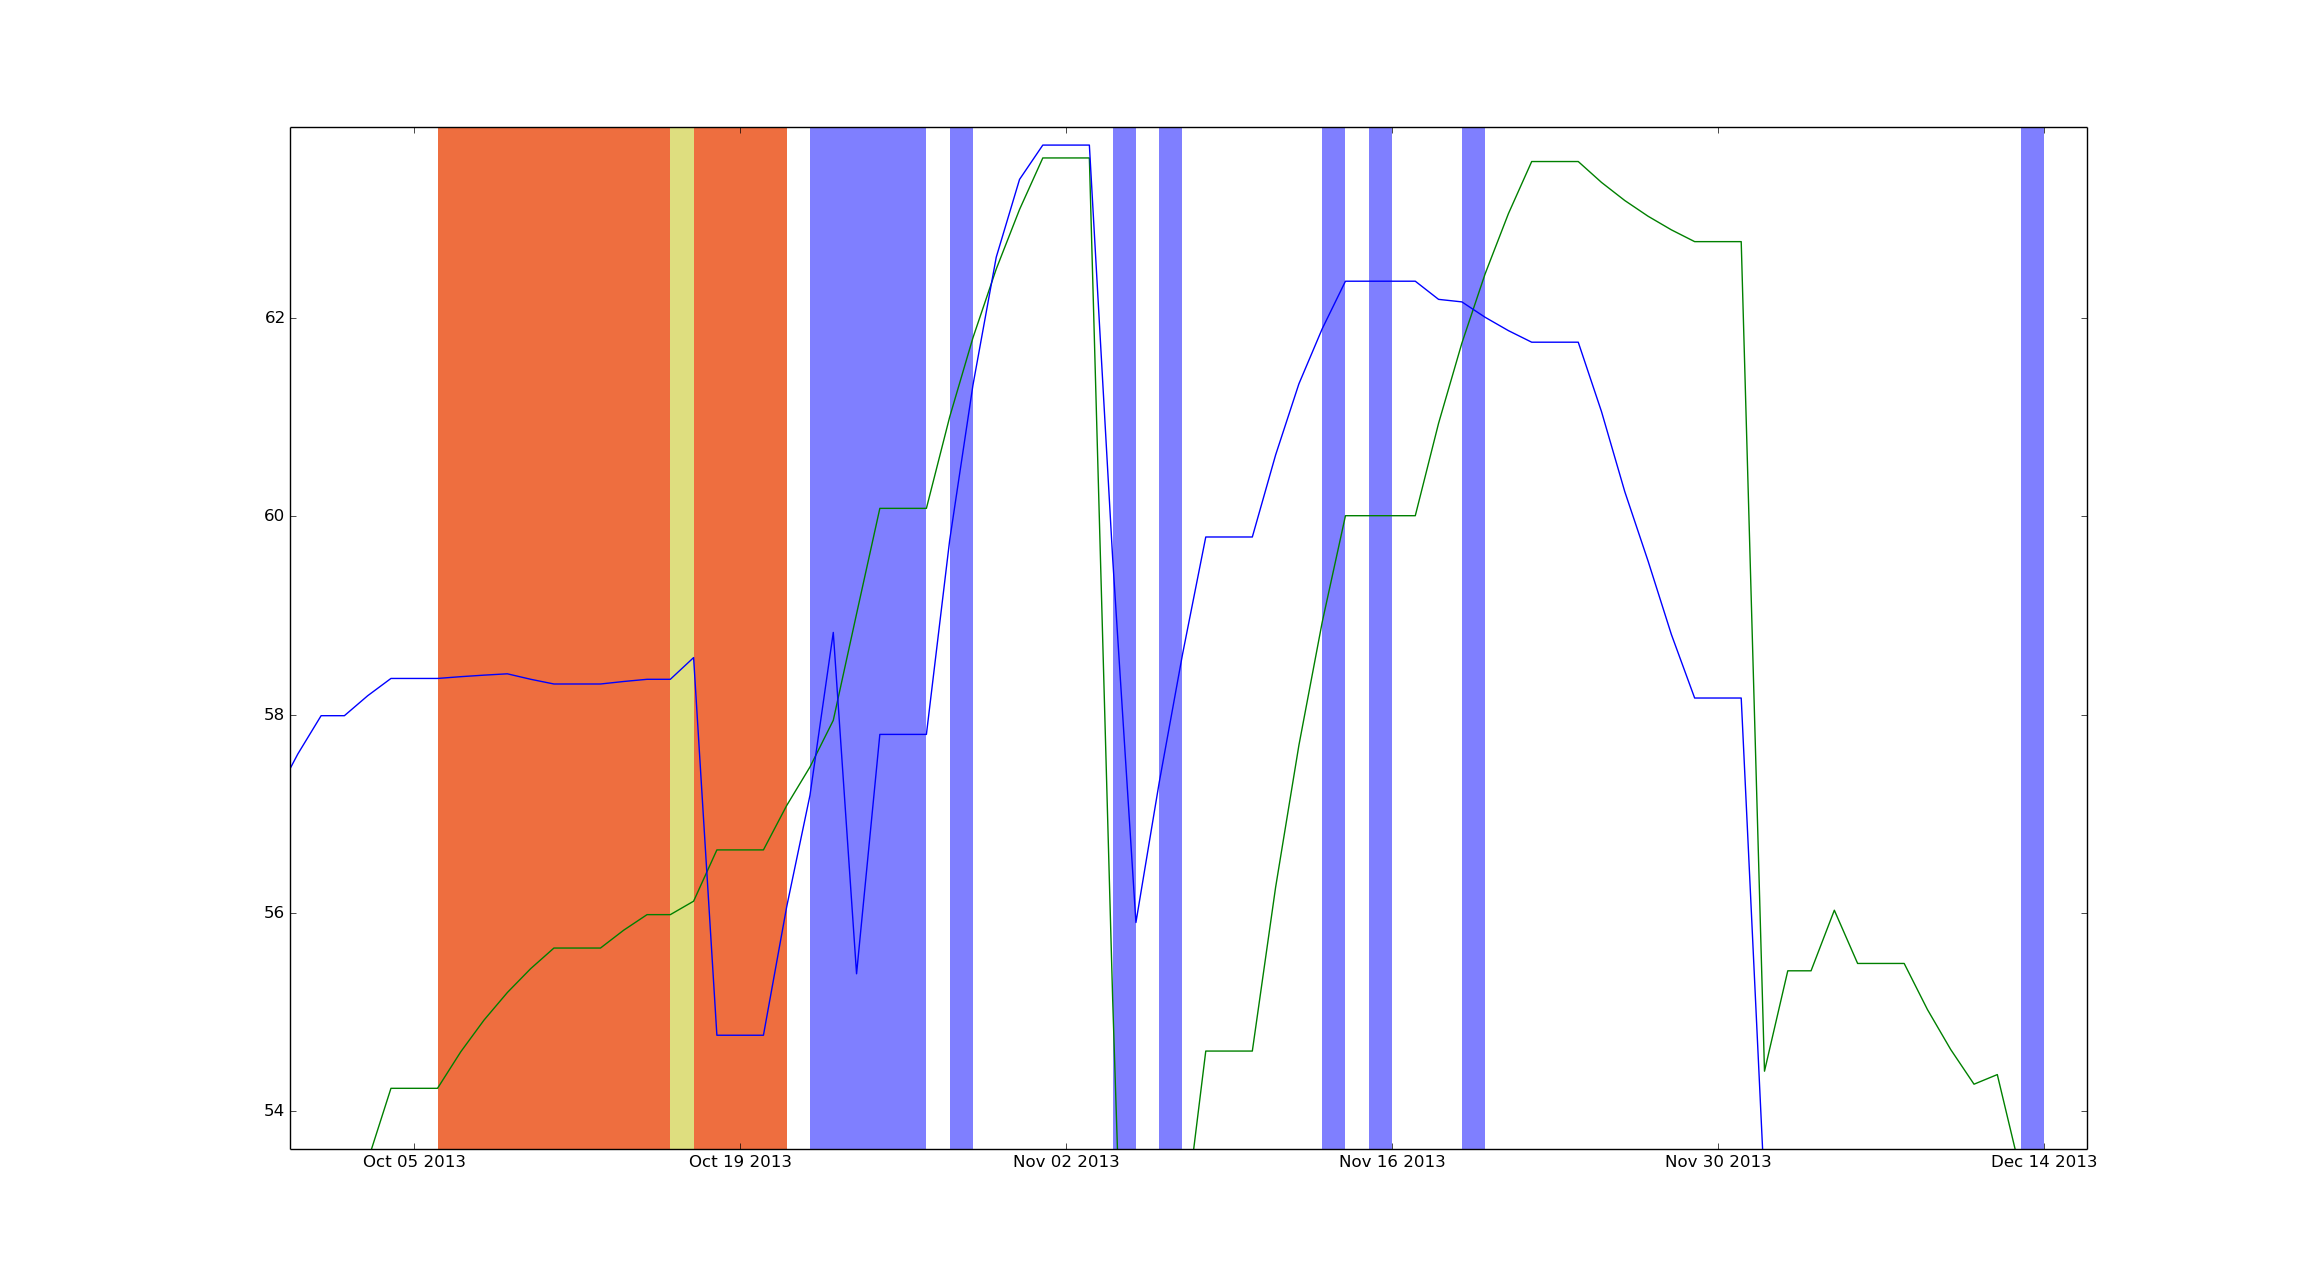
\includegraphics[width=0.8\textwidth]{graphs/20131006_1015_1021.png}
		    	\caption{Window based correlation (Green line - Centre Retail Price, Blue Line - Average Retail Price)}
		    	\label{fig:20131006_1015_1021}
			\end{figure}
						
		\end{itemize}
		
		Other interesting observations that were found while conducting above mentioned tests are as following:
		\begin{itemize}
			\item The lag chosen while comparing retail and arrival for Mumbai came as 15 days which means it takes 15 days of time for arrival to impact retail.
			\item The lag chosen by method while comparing retail and arrival for Delhi came out to be -9 days which gives hints that retail prices are impacting arrival of Onion which is not ideal in real time scenario.
			\item The lag chosen while comparing retail and wholesale for Mumbai comes out as -15 which means retail prices are impacted in approx. 15 days after change in the wholesale prices.
			\item The lag chosen while comparing retail and wholesale for Delhi comes out as -4 which is clearly very small than Mumbai. It might be because of smaller supply chain in Delhi compared to Mumbai.
			\item The lag chosen while comparing wholesale and arrival for Mumbai came as 11 days which means it takes 11 days of time for arrival to impact wholesale.
			\item The lag chosen by method while comparing wholesale and arrival for Delhi came out to be -14 days which gives hints that wholesale prices are impacting arrival of Onion which is not ideal in real time scenario.
		\end{itemize}
		
		Limitations of method:
		\begin{itemize}
			\item The method reports all the tenures where series are not in sync or are in sync(as needed). Like in case of  2008-03-06 to 2008-03-20 for retail vs average, though the correlation went really high because of opposite directions but the fluctuation in prices were not very prominent.
			\item If all the timeseries follows same anomalous behavior then it is not possible to find anomaly in any.
			\item If the anomaly is for very small tenure compared to the selected window size then it is likely to be missed or go unnoticed. In case of 2011-01-06 - 2011-01-08
		\end{itemize}

\subsection{Multivariate Time Series- Vector Autoregressive}

		The method uses vector autoregressive framework for multivaraiate time-series analysis in order to forecast values by using all the related variables/timeseries that can impact the timeseries. The error in the predicted value with the original value helps in determining anomalous points from the timeseries. MAD test is applied in order to fix the threshold value for the error.
		60\% (This can be configured as per need) of the data is used for calibration and rest of the data is checked for anomalous points. So, the start date for the anomalous points begins after 2011-09-16
		\\
		The function is tested with different set of timeseries. Following are the four tests which were performed:
		\begin{enumerate}
		    \item \textbf{Retail Price vs Average of Retail Price}: All the centres should ideally move in tandem. So test is performed over every centre with other centres helping in predicting values.            
		    \item \textbf{Retail Price vs Arrival of Onion}: Arrival is one of the major deciding factor for retail. So the predictions are made for retail based on arrival.
		    \item \textbf{Retail Price vs Wholesale Price}: Retail prices are predicted based on the wholesale prices.
		    \item \textbf{Wholesale Price vs Arrival of Onion}: Wholesale timeseries is predicted on the basis of arrival timeseries.
		\end{enumerate}
		
		Observations when retail price timeseries is compared with average of retail price timeseries: 
		
		\begin{itemize}
			\item The threshold selected by this method for error values are -19.0358099572 and 107.697818954 which means all the data points with error values less than -19.0358099572 and greater than 107.697818954 are reported by the method.
			
			Some of the tenures for which the method reported anomalies are:
			
			\begin{itemize}
				\item 2013-07-19 to 2013-09-11 (See Figure \ref{fig:20130719_0911})
				\item 2013-09-17 to 2014-01-06 (See Figure \ref{fig:20130917_0106})
				\item 2014-12-03 to 2014-12-15 (See Figure \ref{fig:20141203_1215})
			\end{itemize}
			\begin{figure}[H]
		    	\centering
  		    	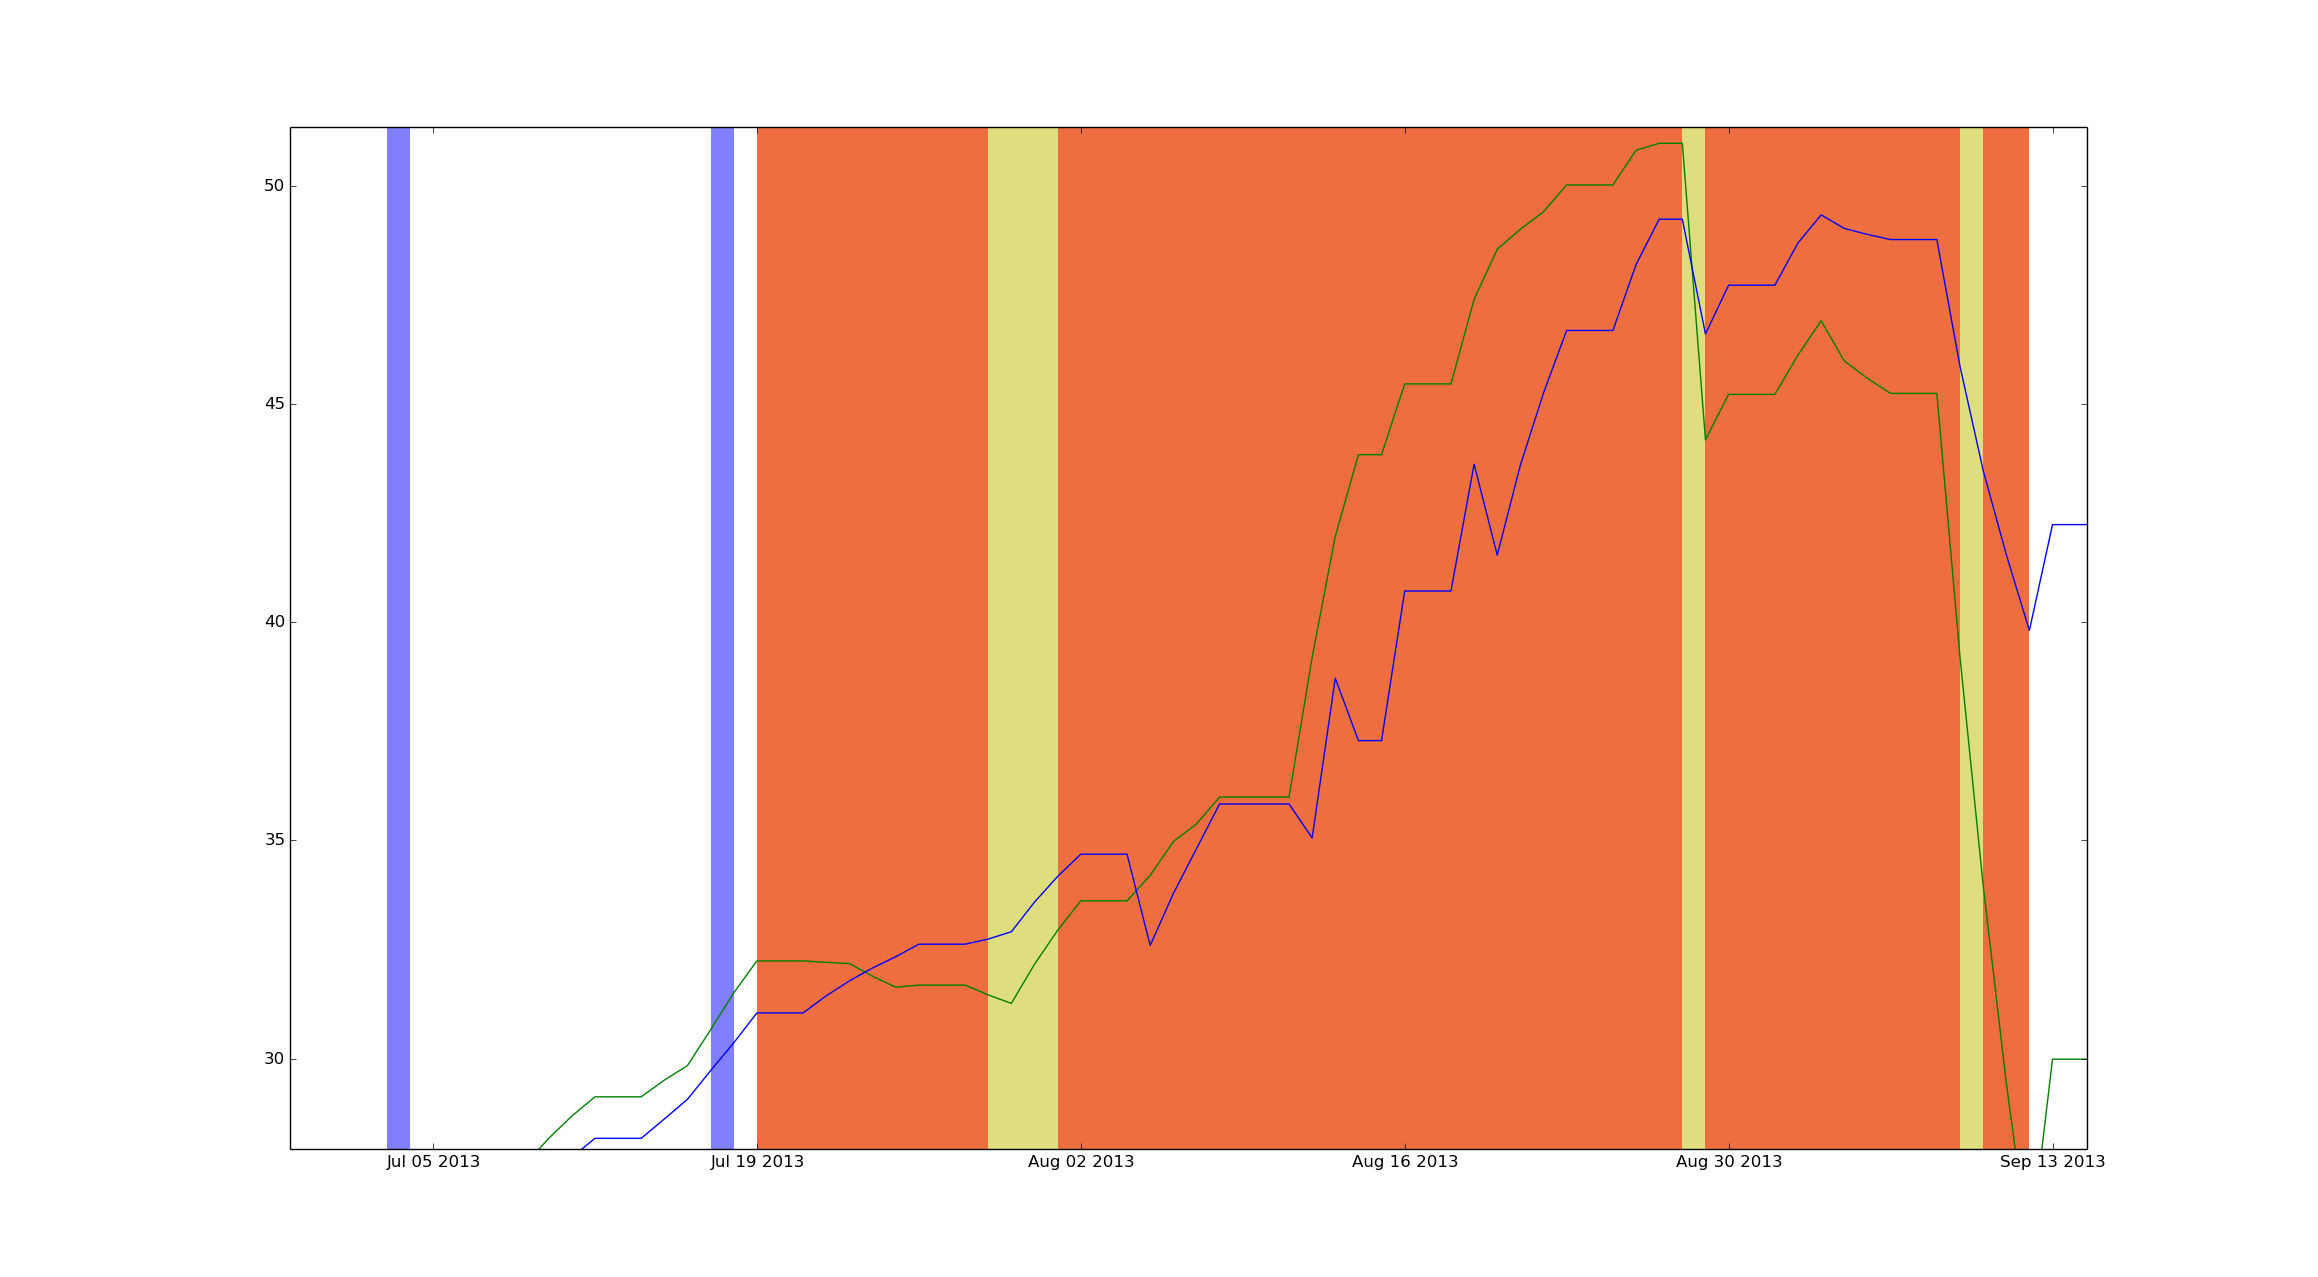
\includegraphics[width=0.8\textwidth]{graphs/20130719_0911.png}
		    	\caption{Vector Autoregressive (Green line - Centre Retail Price, Blue Line - Average Retail Price)}
		    	\label{fig:20130719_0911}
			\end{figure}
			
			\begin{figure}[H]
		    	\centering
  		    	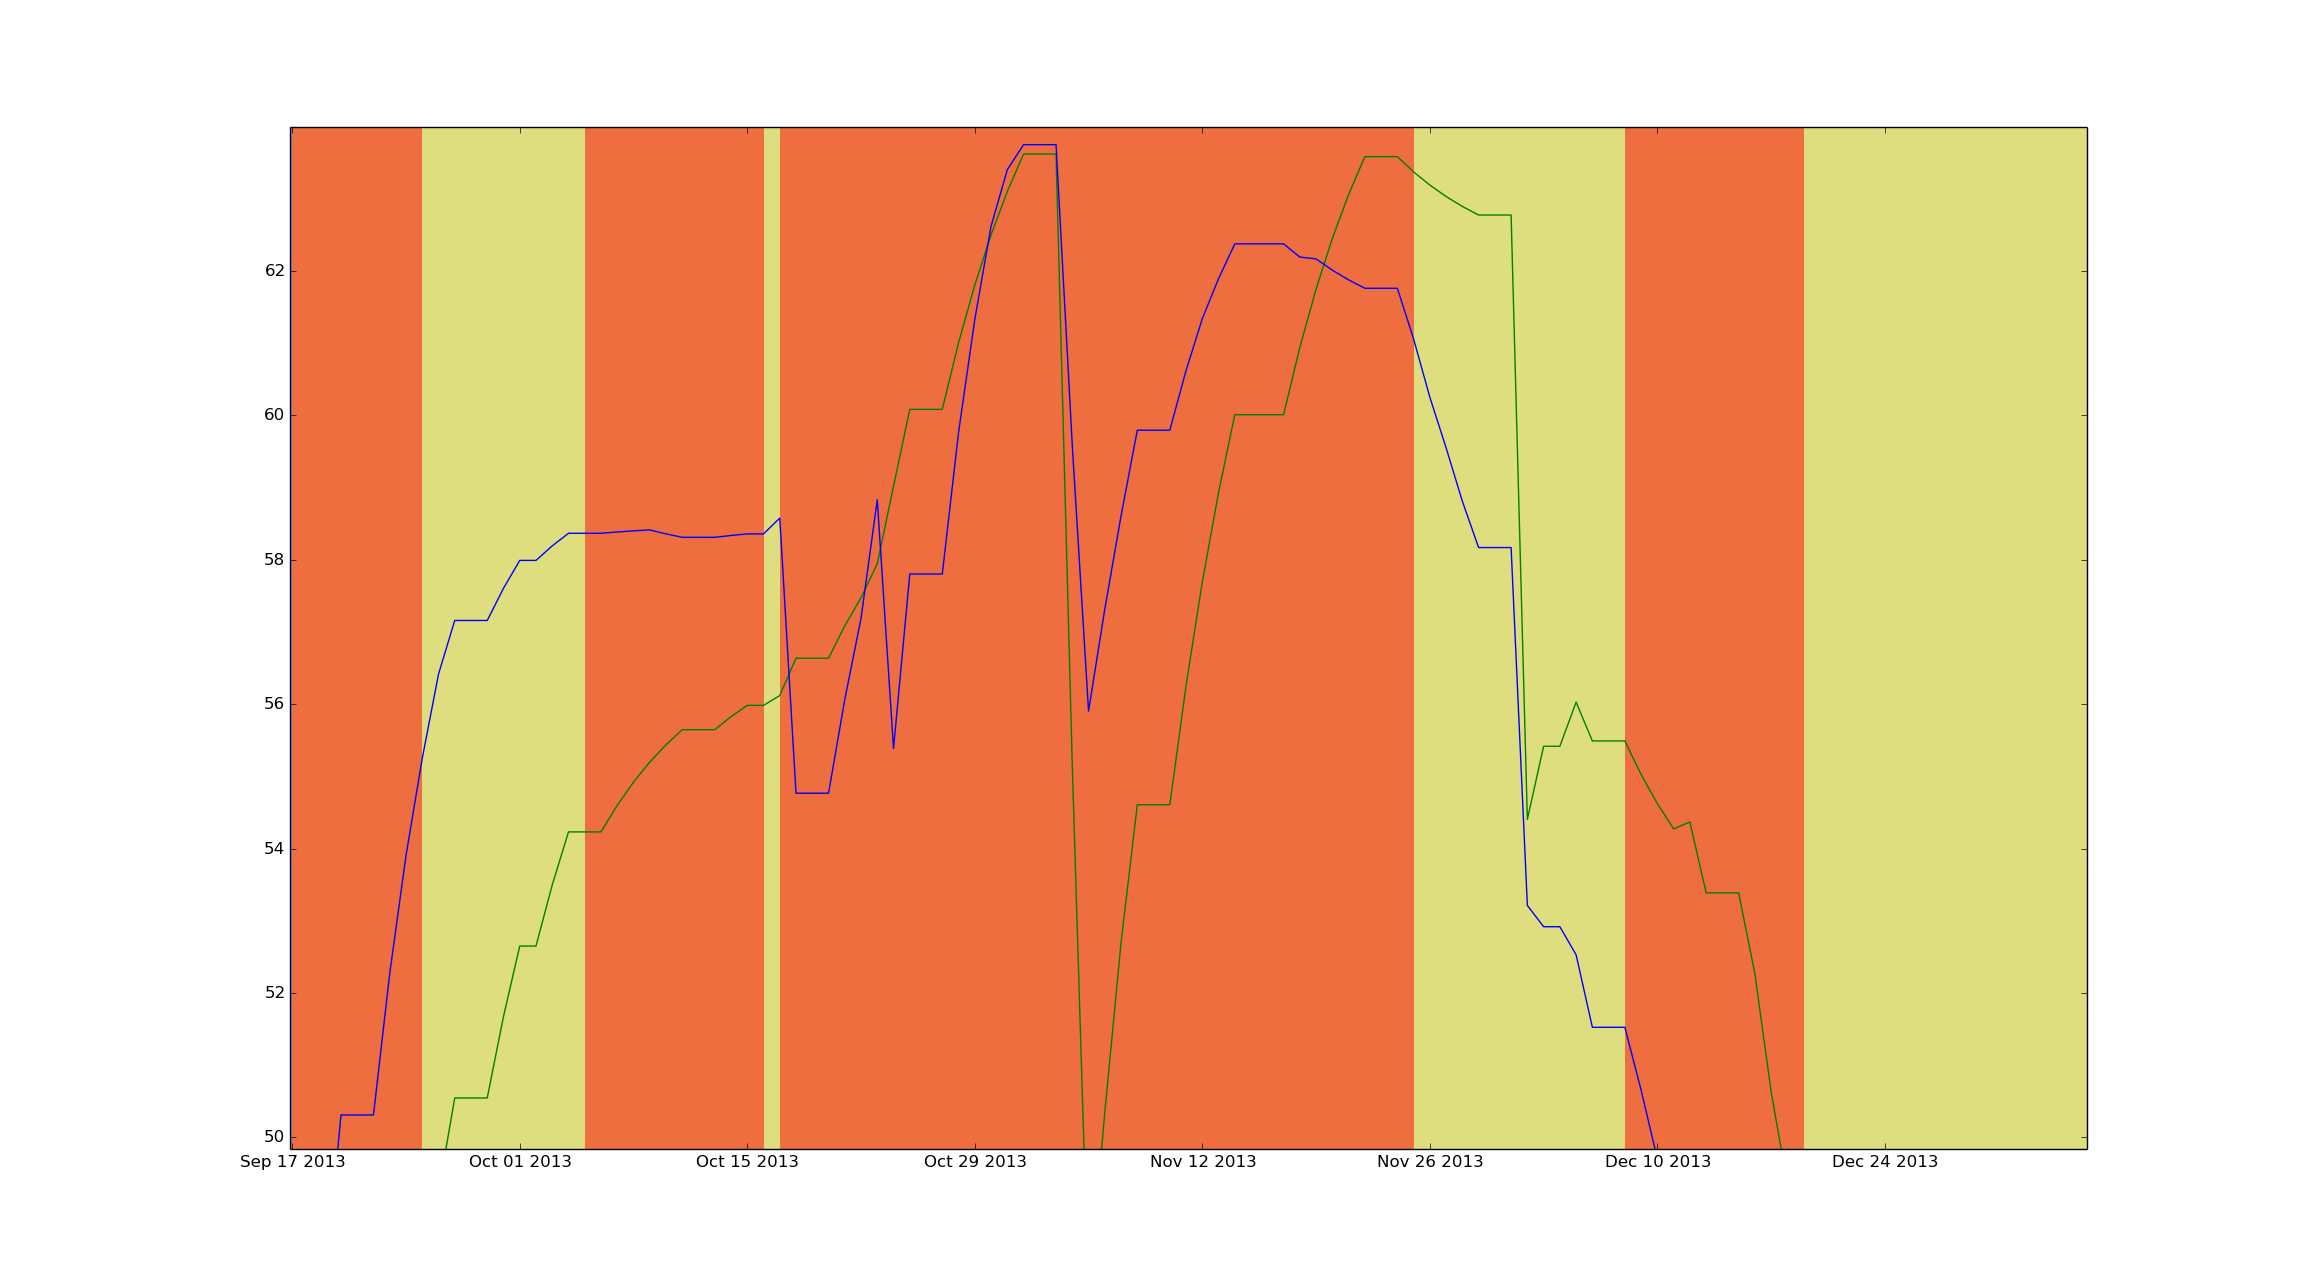
\includegraphics[width=0.8\textwidth]{graphs/20130917_0106.png}
		    	\caption{Vector Autoregressive (Green line - Centre Retail Price, Blue Line - Average Retail Price)}
		    	\label{fig:20130917_0106}
			\end{figure}

			\begin{figure}[H]
		    	\centering
  		    	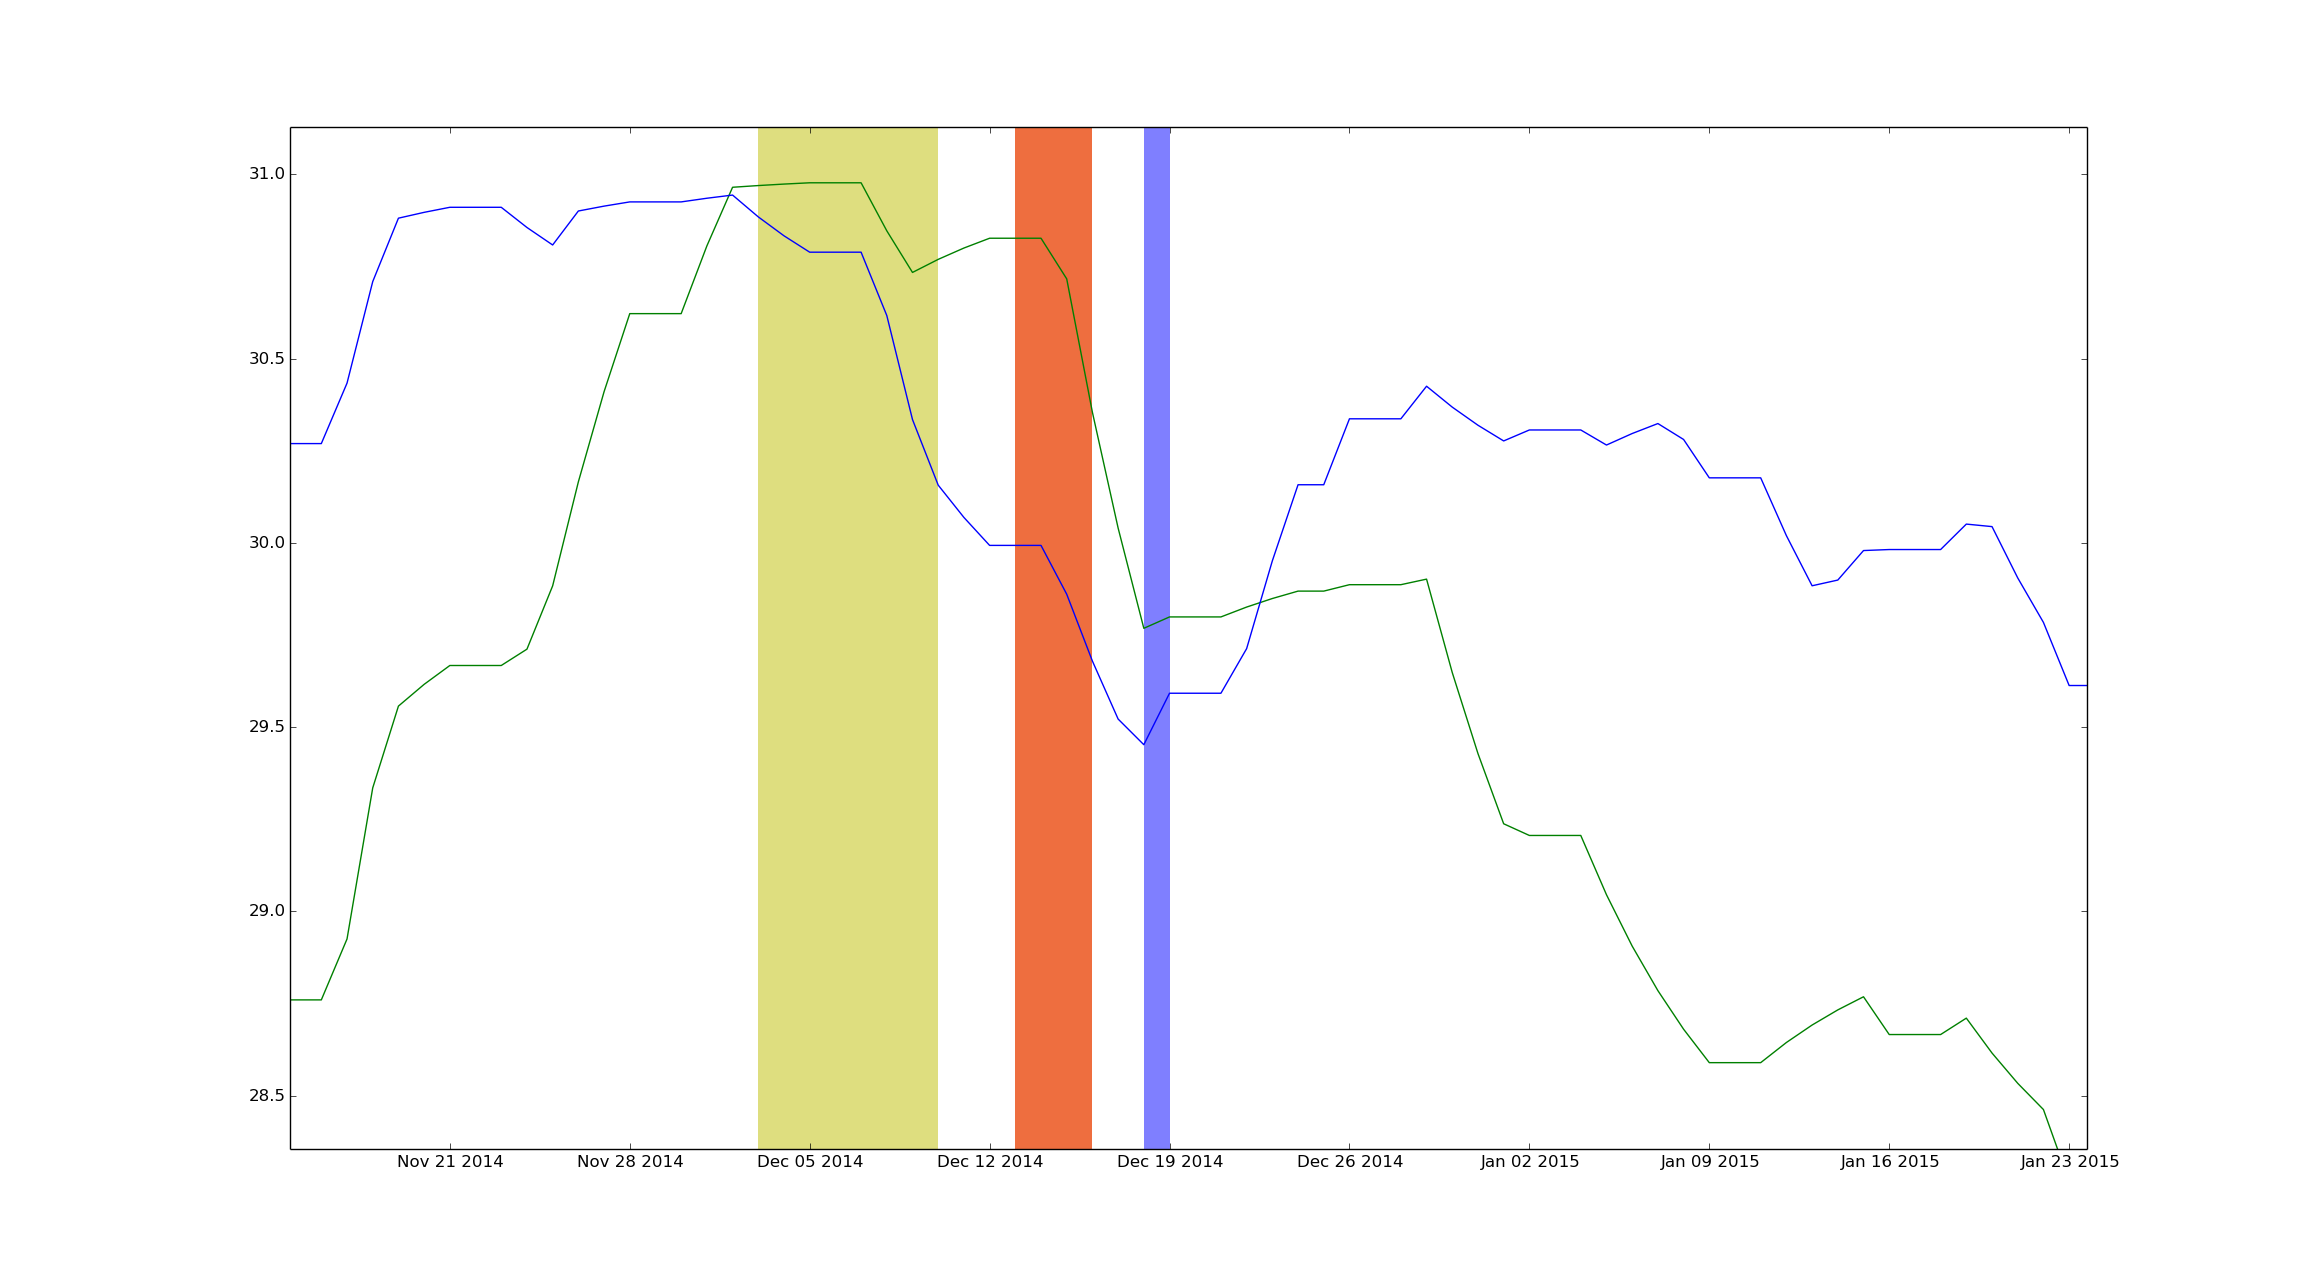
\includegraphics[width=0.8\textwidth]{graphs/20141203_1215.png}
		    	\caption{Vector Autoregressive (Green line - Centre Retail Price, Blue Line - Average Retail Price)}
		    	\label{fig:20141203_1215}
			\end{figure}
			
			No data points were reported against news articles present in May, June, July 2014 despite of large error value. The threshold selected by the MAD test was higher than the error values. This could be corrected by manually setting threshold values which can be account for these data points.
			
		\end{itemize}
		
		Other interesting observations that were found while conducting above mentioned tests are as following:
		\begin{itemize}
			\item Some of the data points like July 2014 data were not captured despite of error value close to MAD threshold. These can be captured by lowering the threshold.
			\item For news articles in Dec 2012,Jan 2013, Feb 2013 the values does not show high error values despite of news articles reporting the crisis. The possible reason could be because similar trend have been seen for this tenure in the data.
		\end{itemize}
		
		Limitations of method:
		\begin{itemize}
			\item The method depends on the MAD Test in order to set threshold. So, even though the error value is close to threshold but less than it won't be reported. Other methods could be also used in order to decide threshold.
		\end{itemize}		
		
		
\subsection{Graph Based Anomaly Detection}

	This method, treats each day as a node of a graph, and connects with other nodes if nodes are similar. This connecting edge is given similarity value and random walk is performed to get connectivity of each node. Node with the least connectivity values are reported as anomaly. Note that for the previous methods, we had threshold values either defined by user or calculated by using MAD test. But here we do not have that and we just ask method to report "n" number of nodes with least connectivity values.\\
	\\
	The working of this method is quite complex and can not be generalised. For detailed information go through the paper \ref{nasa}. So we will just represent, how method has performed on the different analysis.\\
	\\
	For \textbf{Retail Price vs Average of Retail Price} (See Figure \ref{fig:1231}) and \textbf{Retail Price vs Wholesale Price} (See Figure \ref{fig:12331}), this method has performed well. For \textbf{Retail Price vs Average of Retail Price}, every tenure of anomaly has been matched with some news articles.
	\\
	The anomalies which were not matched with news articles were part of large tenure which had some matching with news articles and usually, this tenure is large and for every date news articles are not present. 
	\\
	Few articles are missed, that might be due to limited number of points chosen. If number of points are increased, than it might be covered as well. 
	\\
	For \textbf{Retail Price vs Wholesale Price}, apart from Jan 2013, July 2014, June 2015, all anomalies are matching with some news articles.\\
			\begin{figure}[H]
		    	\centering
  		    	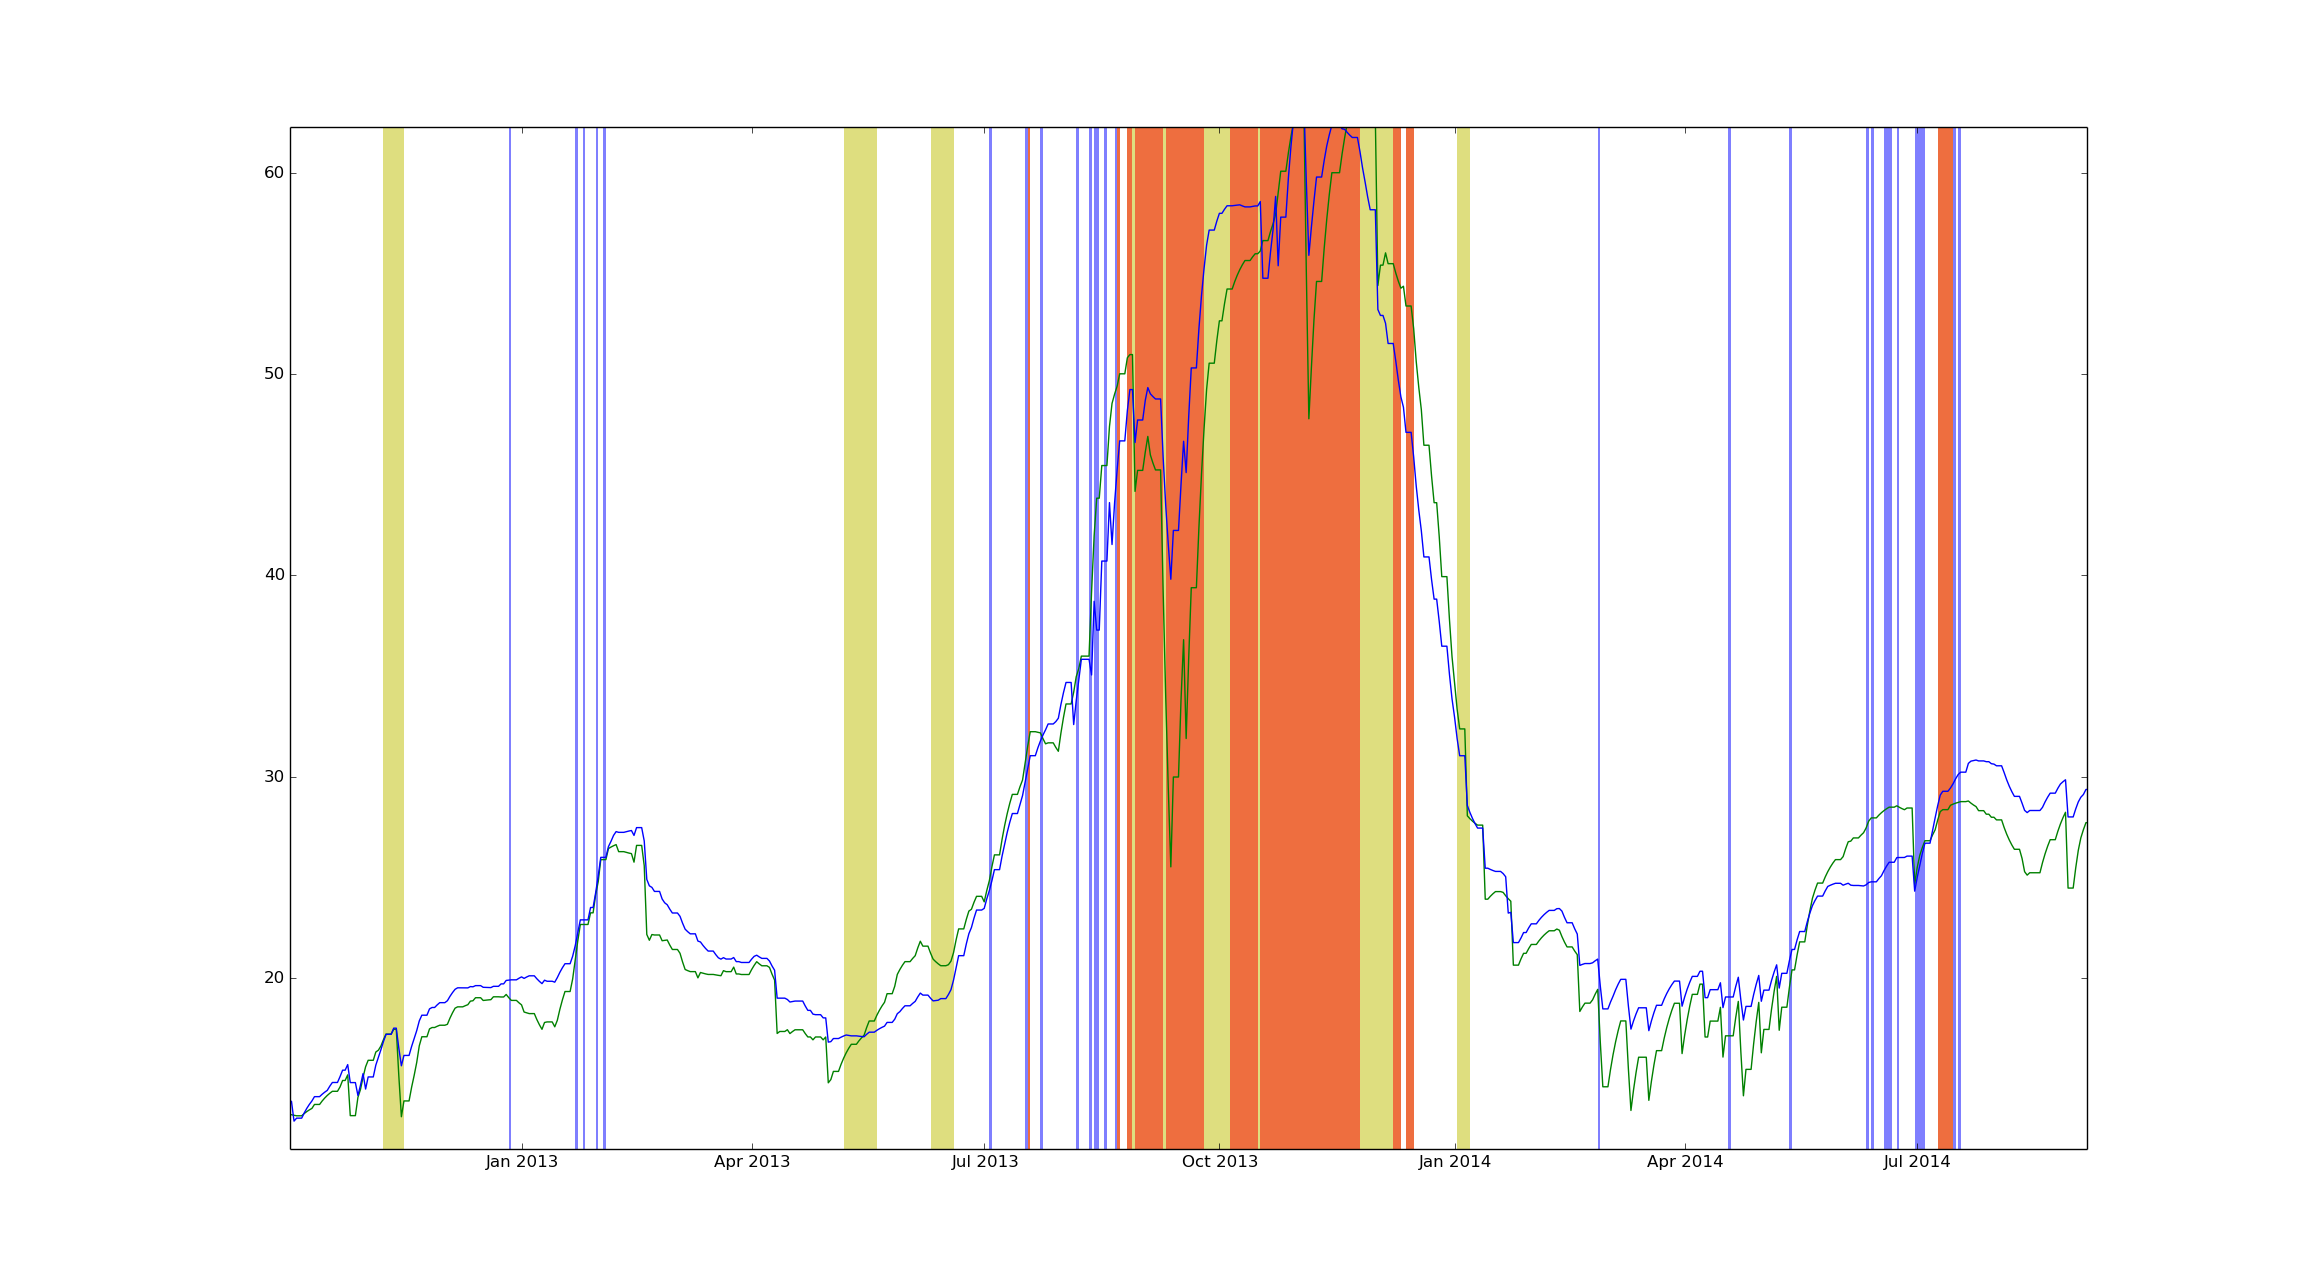
\includegraphics[width=0.8\textwidth]{graphs/1231.png}
		    	\caption{Graph Based Anomaly Detection (Green line - Centre Retail Price, Blue Line - Average Retail Price)}
		    	\label{fig:1231}
			\end{figure}
			
			\begin{figure}[H]
		    	\centering
  		    	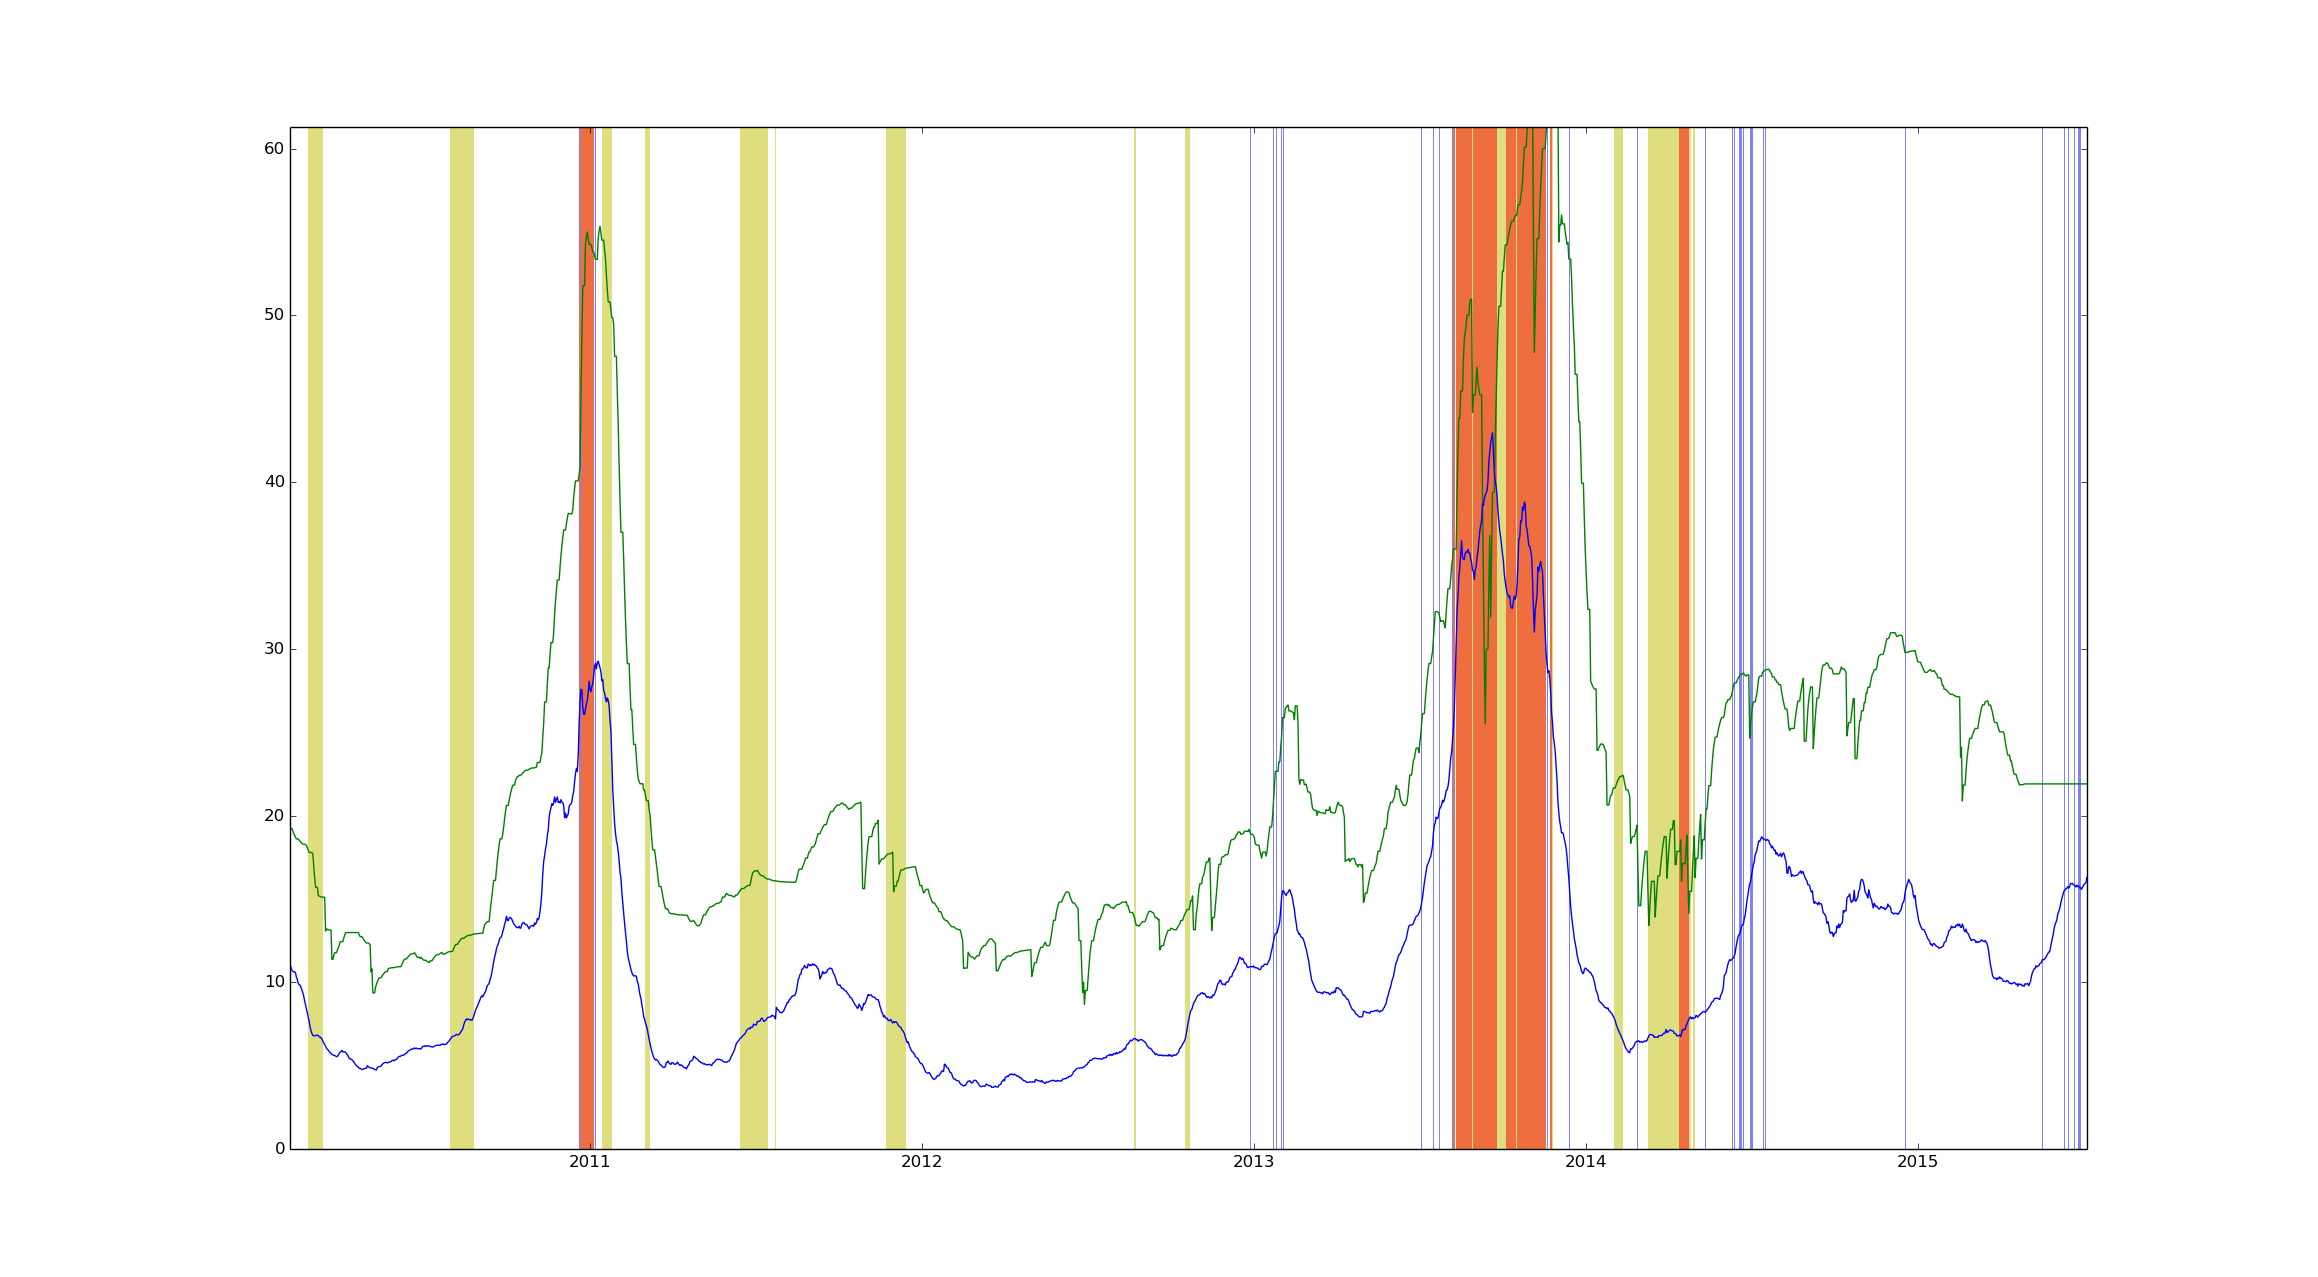
\includegraphics[width=0.8\textwidth]{graphs/12331.png}
		    	\caption{Graph Based Anomaly Detection (Green line - Retail Price, Blue Line - Wholesale Price)}
		    	\label{fig:12331}
			\end{figure}
	
	For \textbf{Retail Price vs Arrival of Onion} (See Figure \ref{fig:12321}) and \textbf{Wholesale Price vs Arrival of Onion} (See Figure \ref{fig:12341}), this method is not producing good results. Many points are reported as anomaly which are close to each other. And due to limited number of points, number of anomalies matching with news articles are quite less. The reason might be because of fluctuations seen in the arrival timeseries. Figures \ref{fig:12322_delhi} and \ref{fig:12442_delhi} describe results of these both analysis for Delhi centre.
			\begin{figure}[H]
		    	\centering
  		    	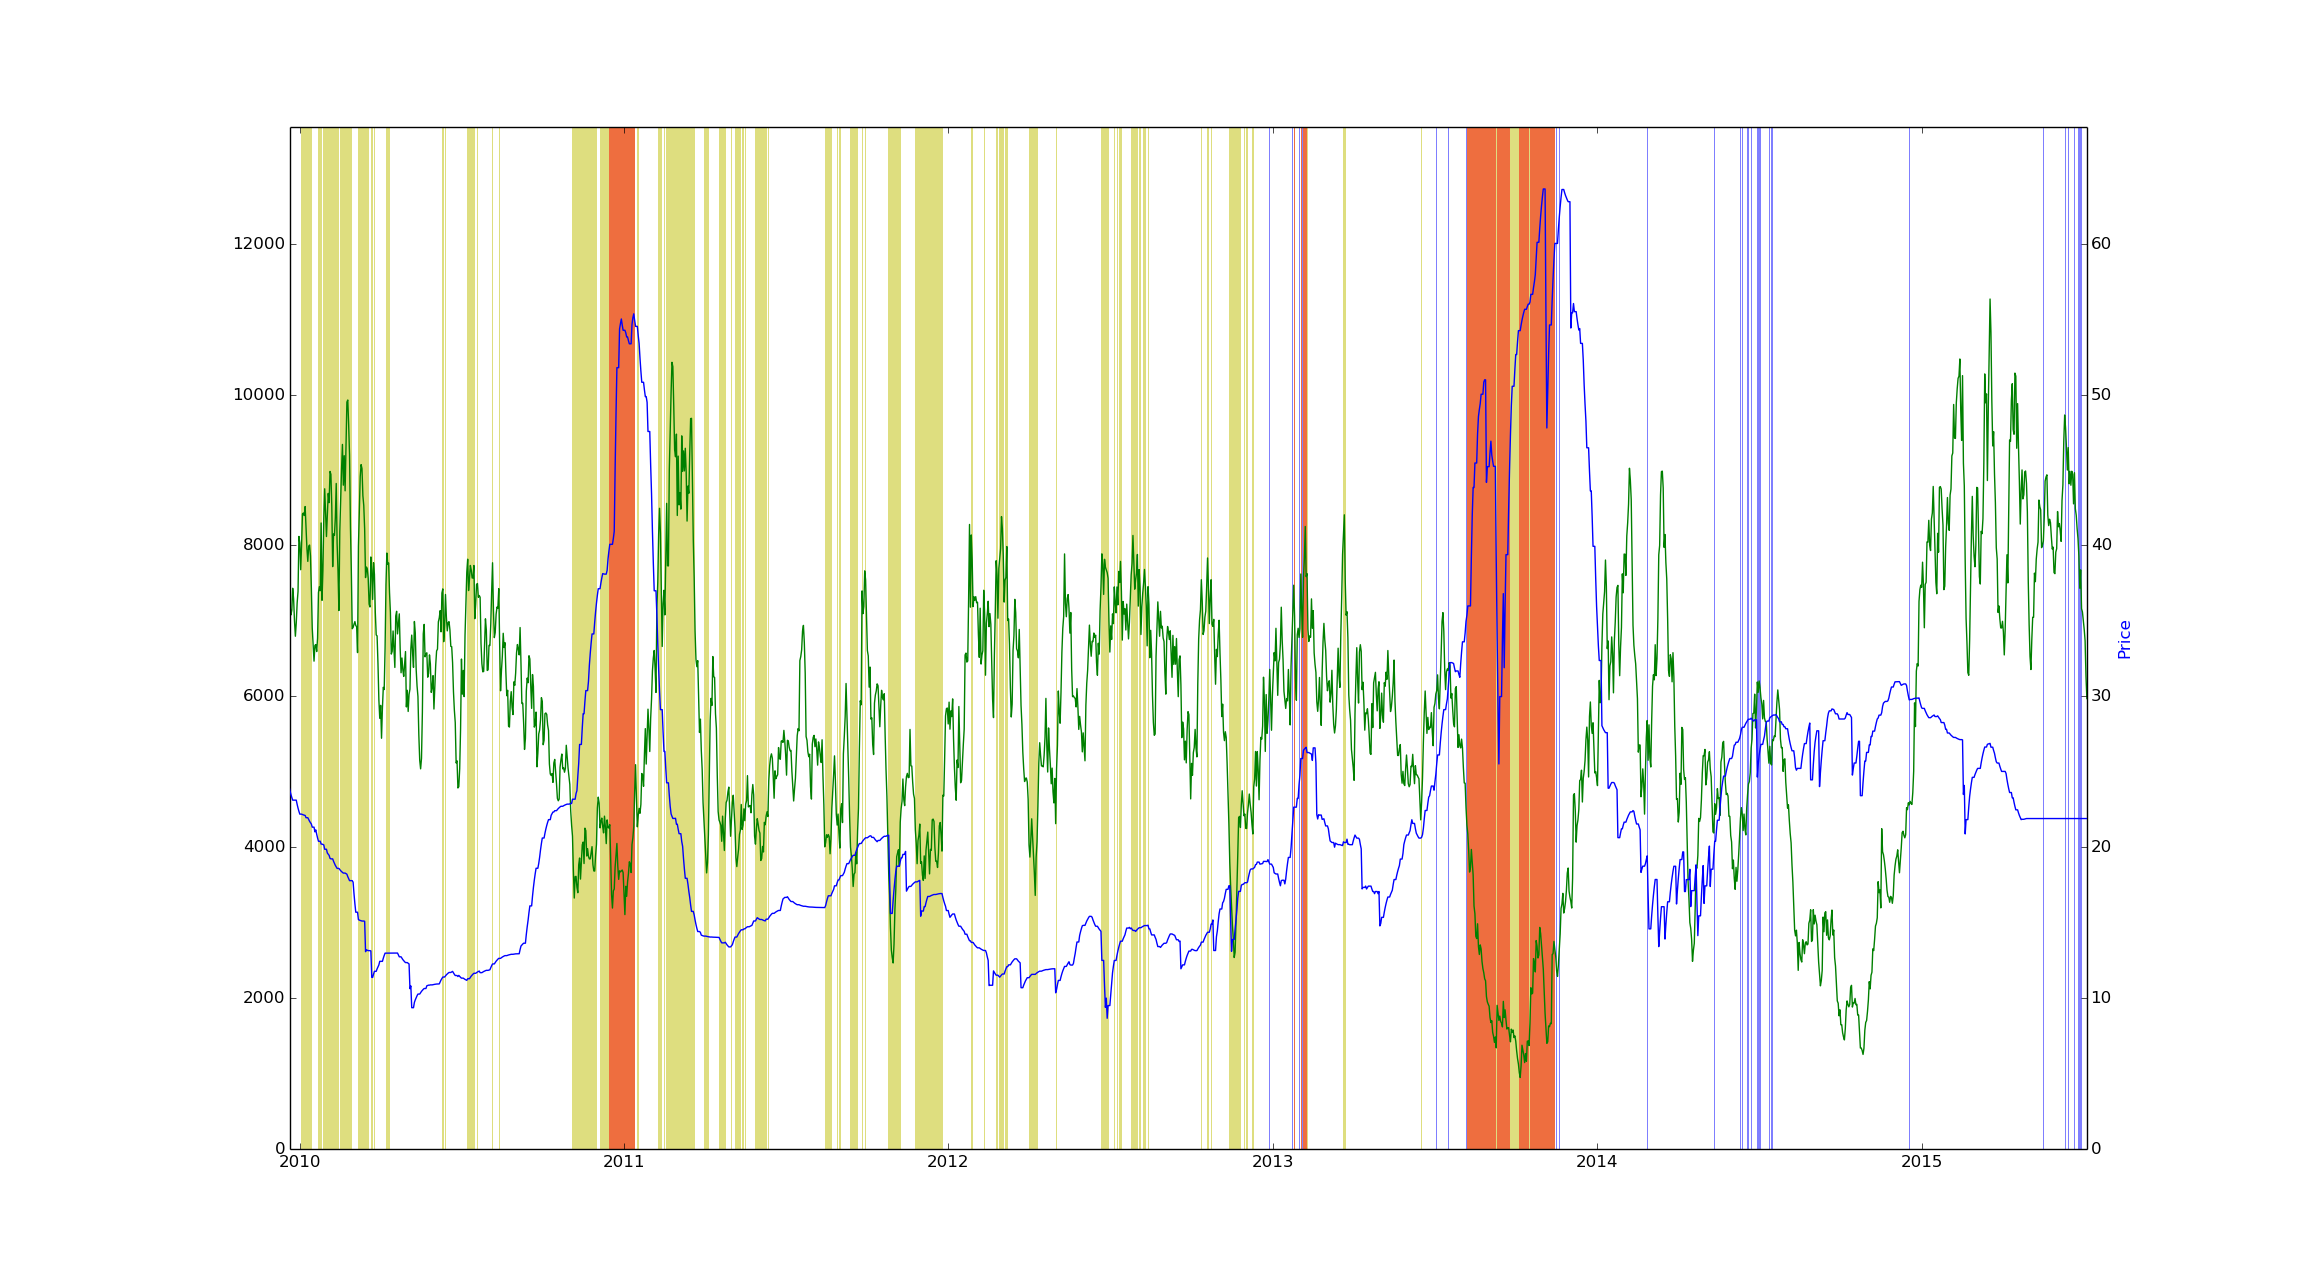
\includegraphics[width=0.8\textwidth]{graphs/12321.png}
		    	\caption{Graph Based Anomaly Detection (Green line - Arrival Data of Onion, Blue Line - Retail Price)}
		    	\label{fig:12321}
			\end{figure}
			
			\begin{figure}[H]
		    	\centering
  		    	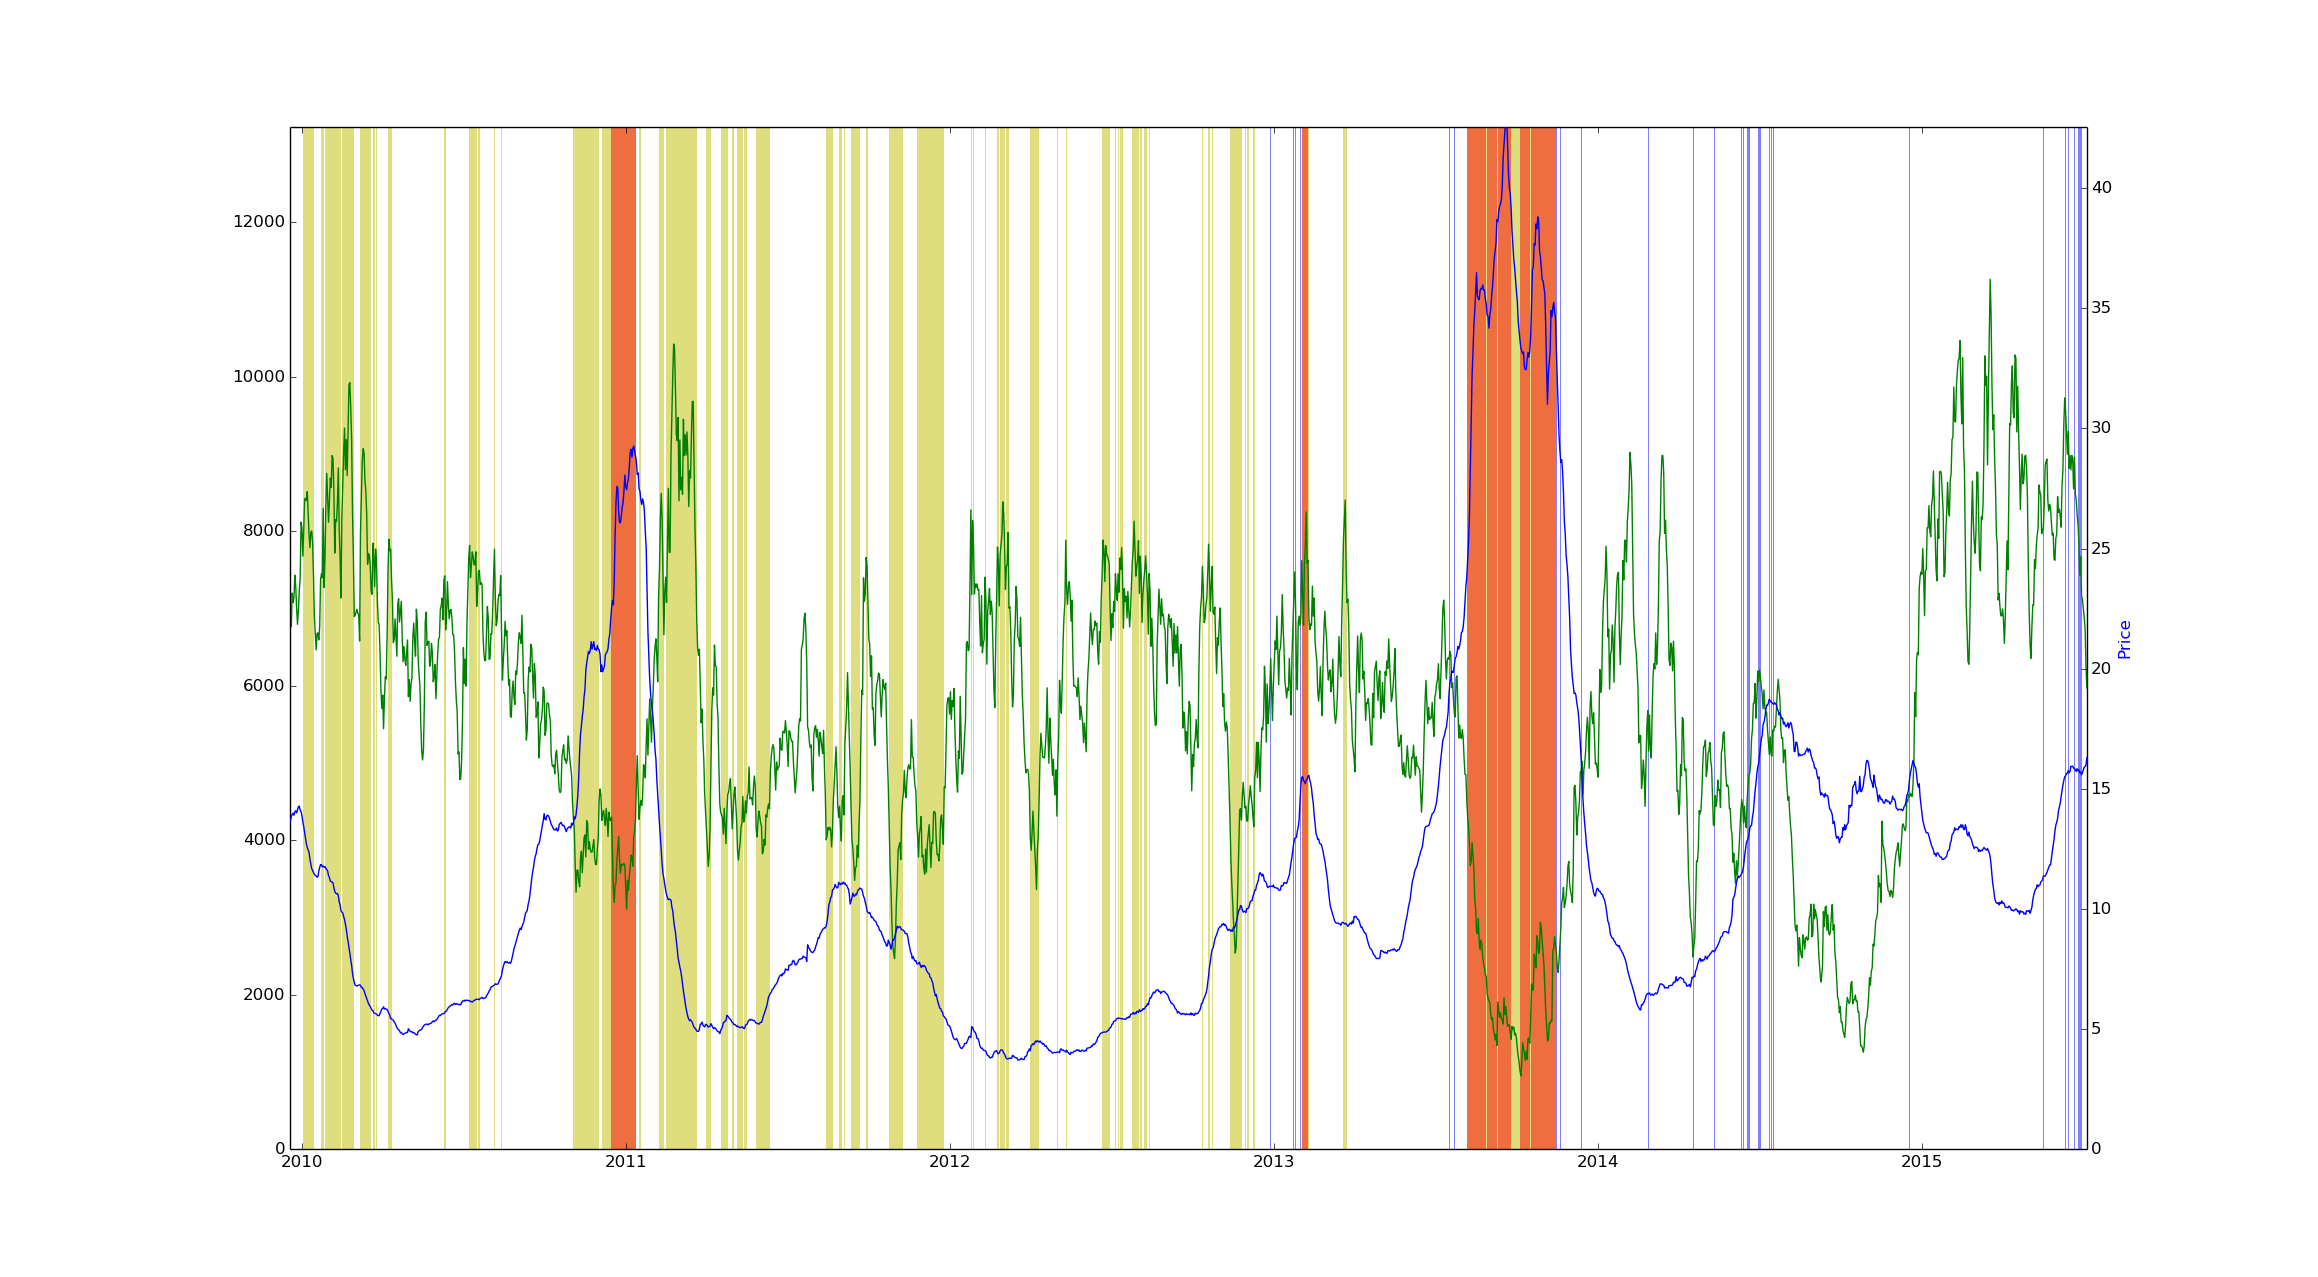
\includegraphics[width=0.8\textwidth]{graphs/12341.png}
		    	\caption{Graph Based Anomaly Detection (Green line - Arrival Data of Onion, Blue Line - Wholesale Price)}
		    	\label{fig:12341}
			\end{figure}
			
			
			\begin{figure}[H]
		    	\centering
  		    	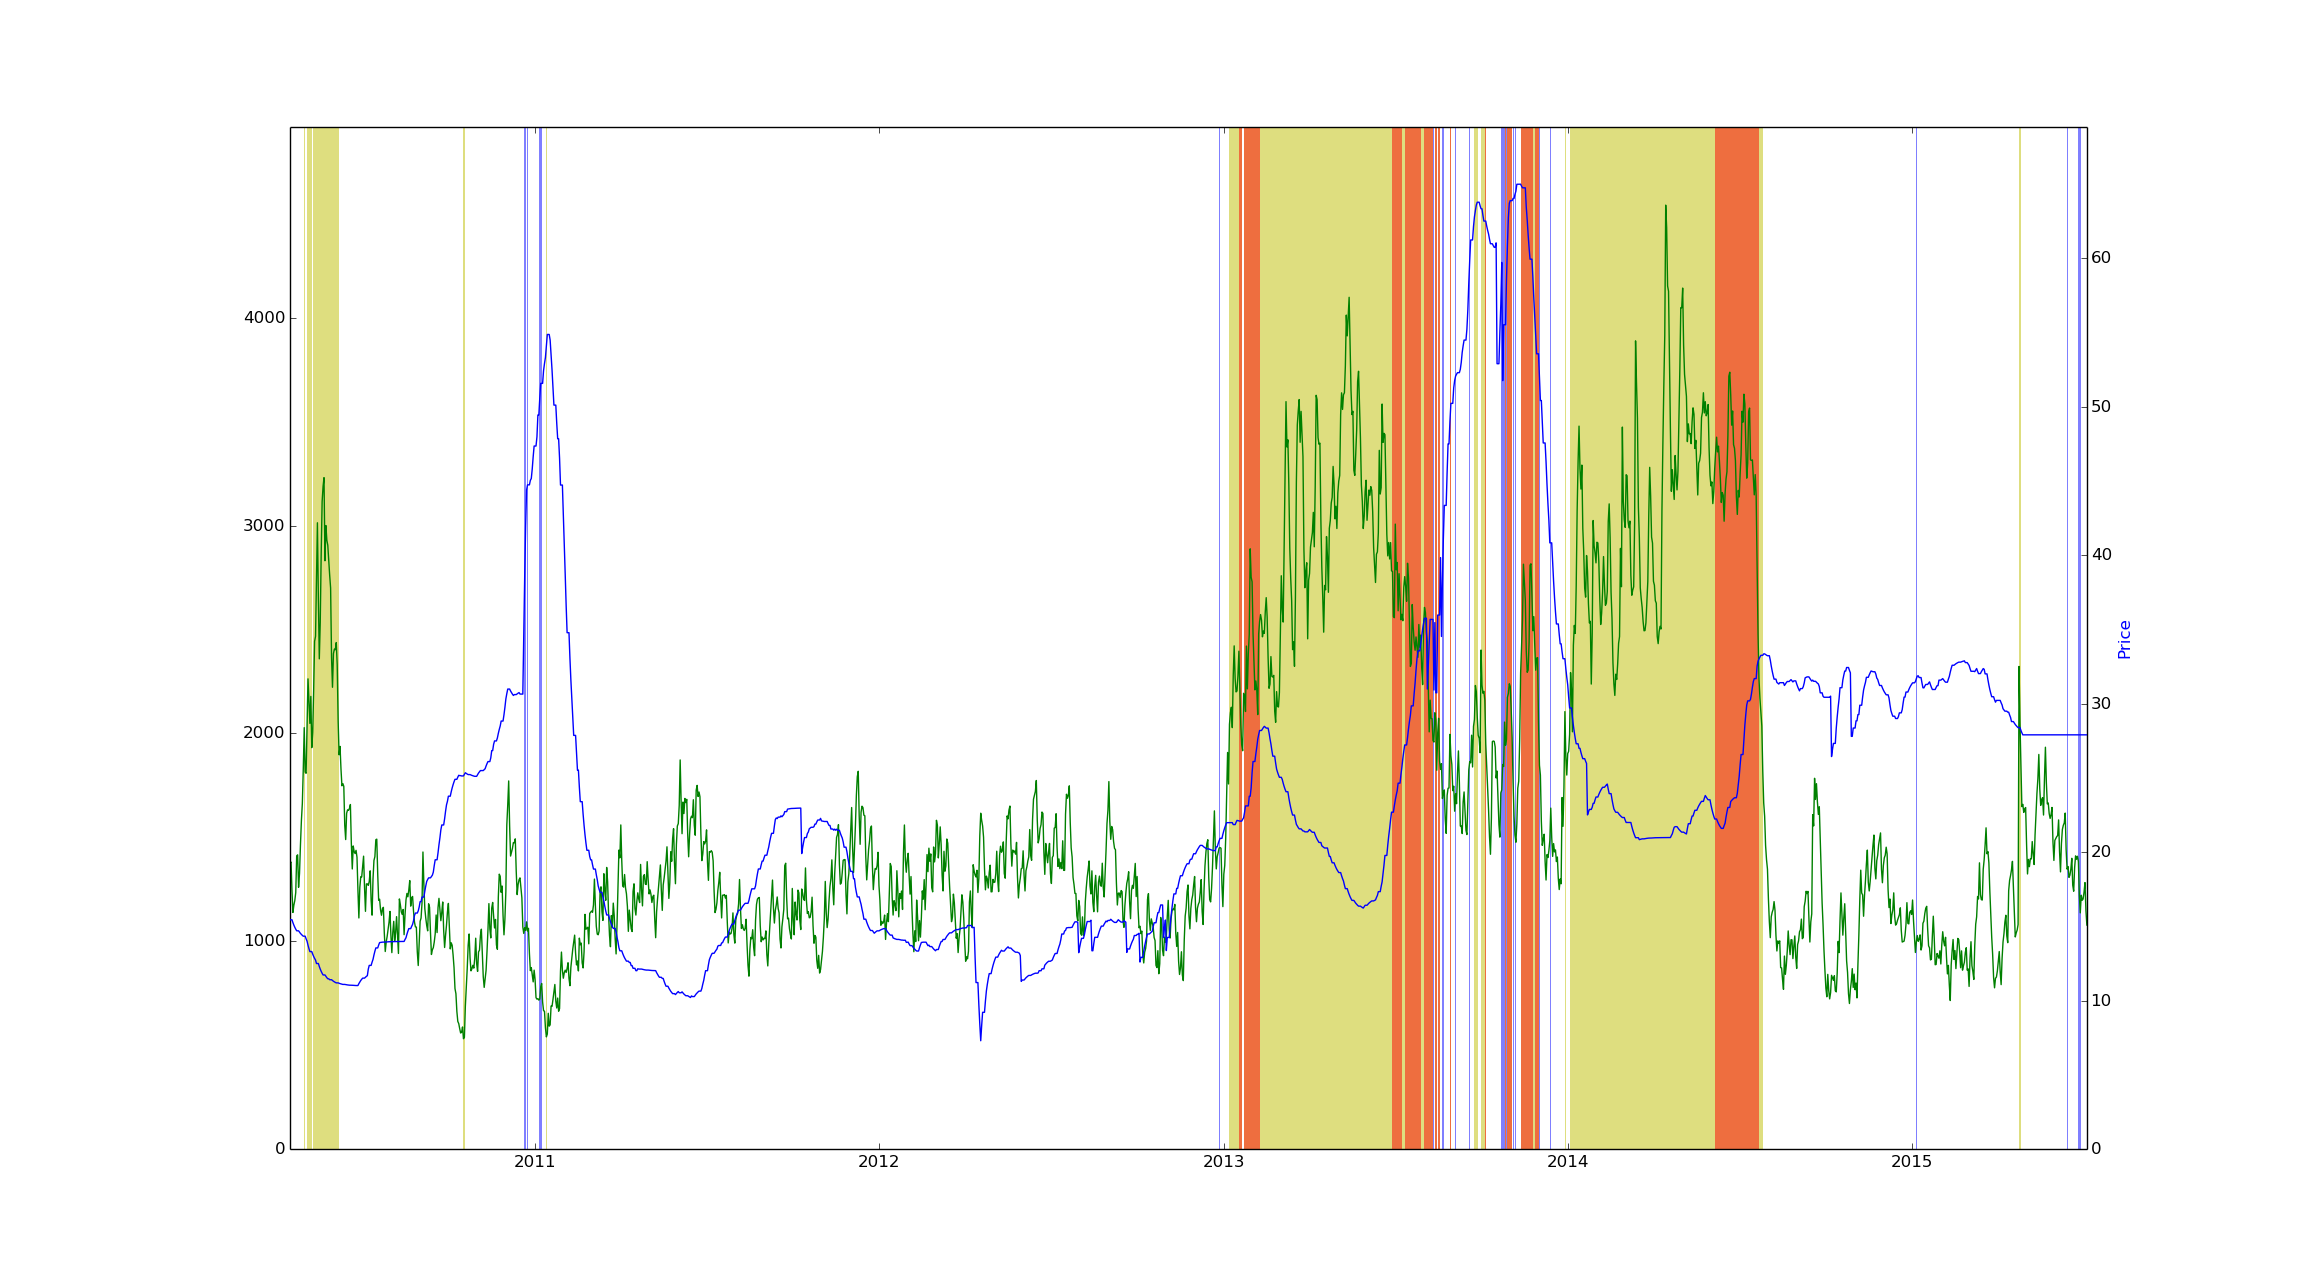
\includegraphics[width=0.8\textwidth]{graphs/12322_delhi.png}
		    	\caption{Graph Based Anomaly Detection (Green line - Arrival Data of Onion, Blue Line - Retail Price)}
		    	\label{fig:12322_delhi}
			\end{figure}
			
			\begin{figure}[H]
		    	\centering
  		    	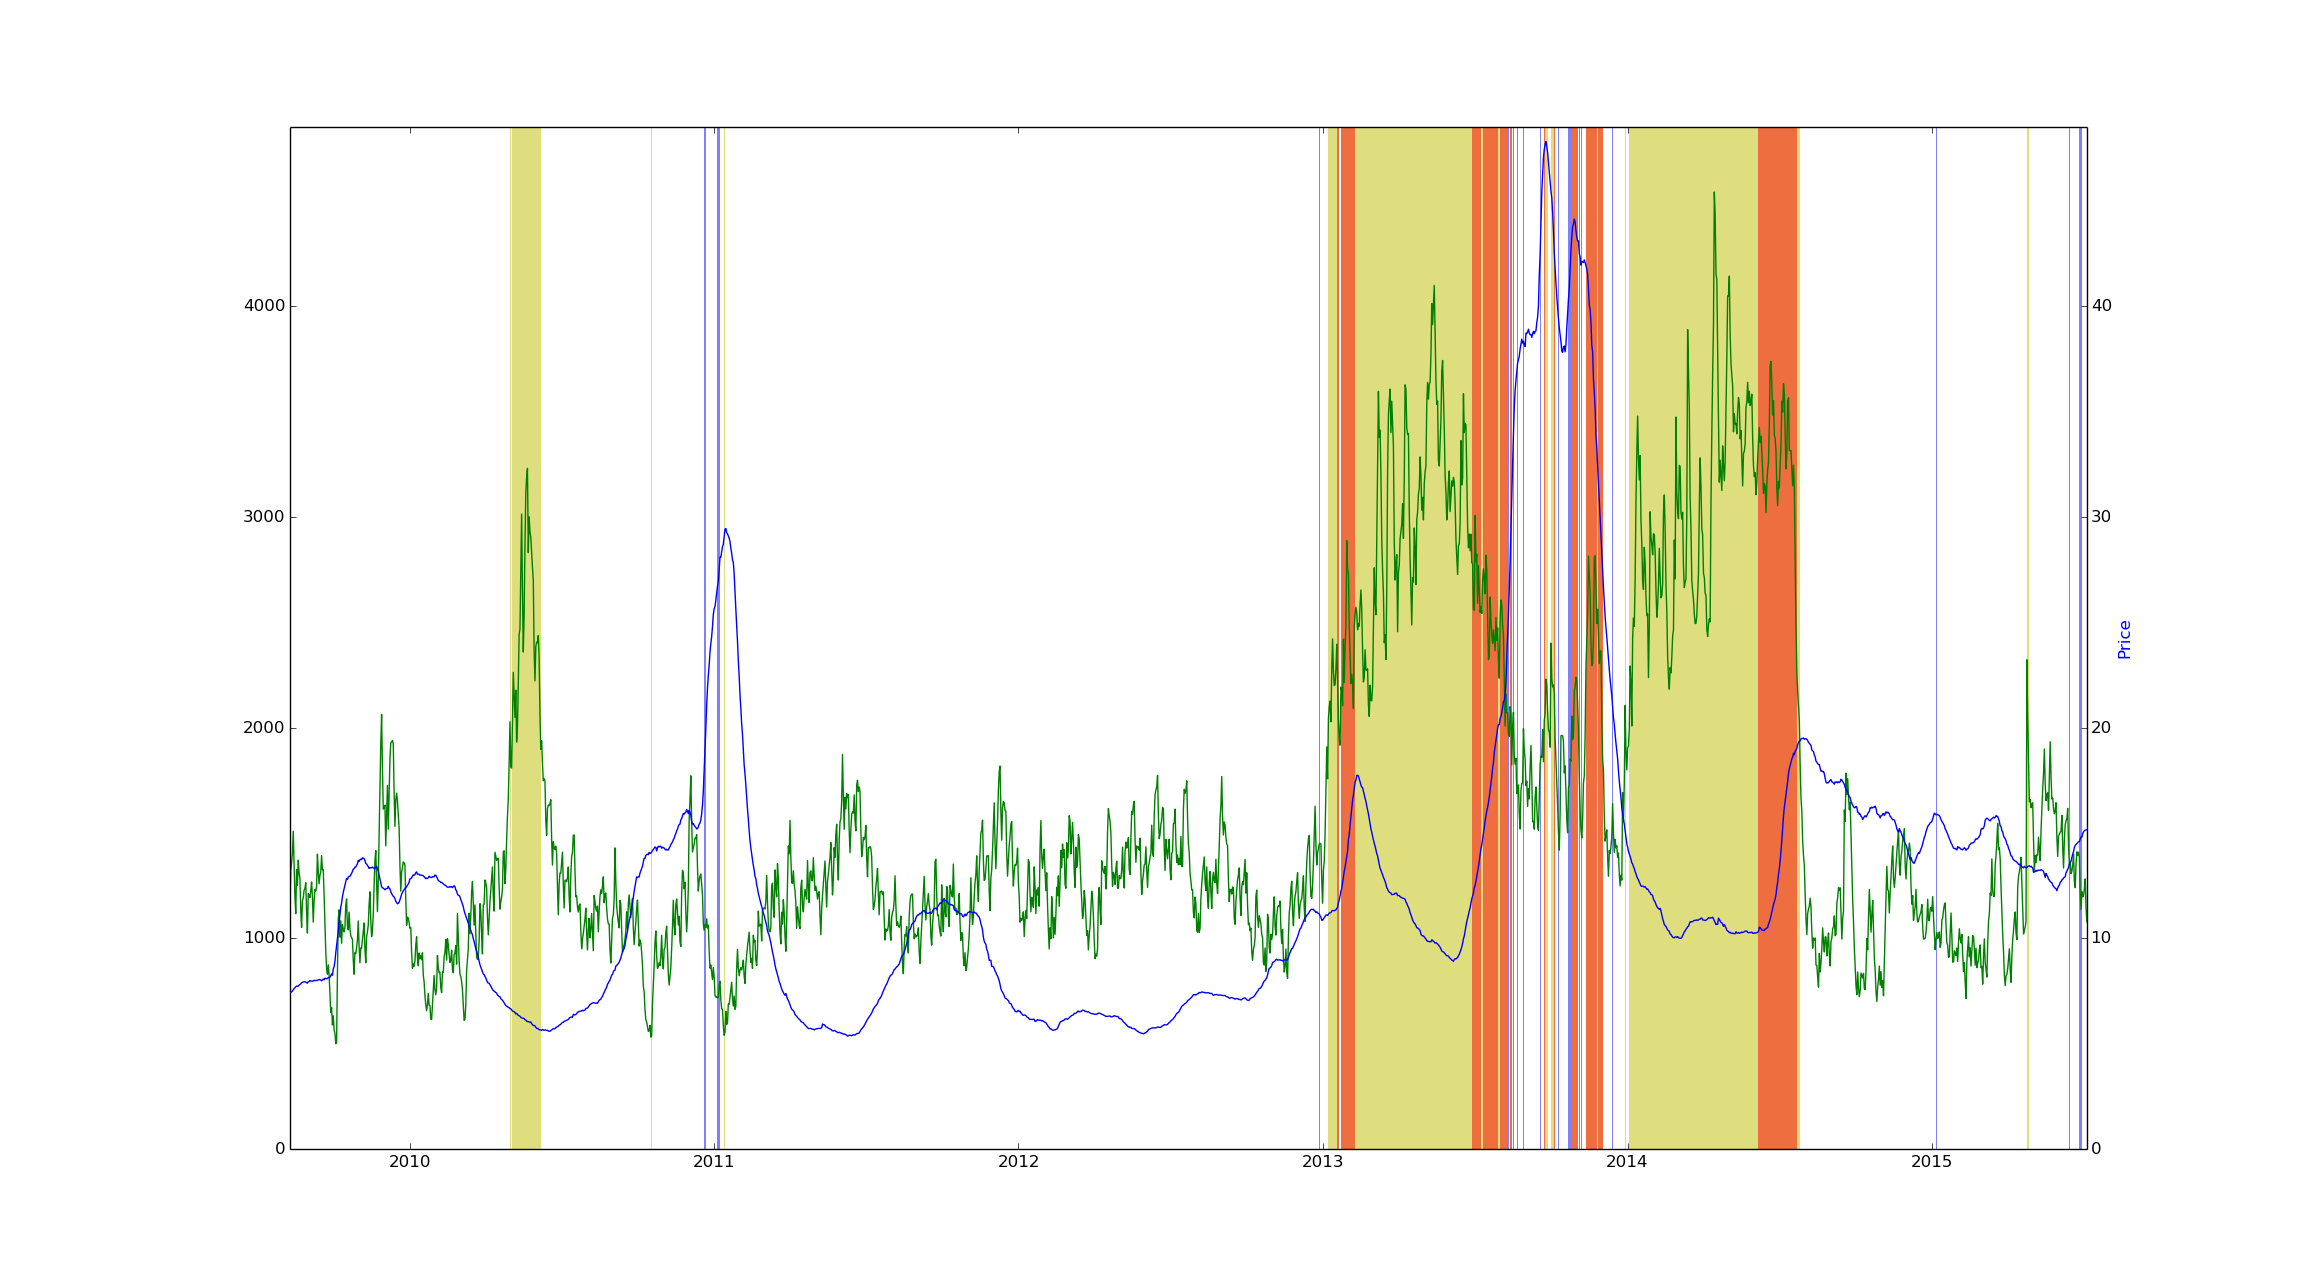
\includegraphics[width=0.8\textwidth]{graphs/12442_delhi.png}
		    	\caption{Graph Based Anomaly Detection (Green line - Arrival Data of Onion, Blue Line - Wholesale Price)}
		    	\label{fig:12442_delhi}
			\end{figure}	